\documentclass[12pt,useAMS]{ociamthesis}  % default square logo 
%\documentclass[12pt,beltcrest]{ociamthesis} % use old belt crest logo
%\documentclass[12pt,shieldcrest]{ociamthesis} % use older shield crest logo

%load any additional packages
\usepackage{amssymb}
\usepackage{footnote, url, amsmath}
\usepackage{natbib}

%define all that you need to define
\def\starpy {\textsc{starpy}}

%input macros (i.e. write your own macros file called mymacros.tex 
%and uncomment the next line)
%\include{mymacros}

\title{The influence of morphology, AGN and environment     %your thesis title,
        on the quenching histories of galaxies}   %note \\[1ex] is a line break in the title

\author{Rebecca Jane Smethurst}             %your name
\college{Pembroke College}  %your college

%\renewcommand{\submittedtext}{change the default text here if needed}
\degree{Doctor of Philosophy}     %the degree
\degreedate{Michaelmas 2016}         %the degree date

%end the preamble and start the document
\begin{document}

%this baselineskip gives sufficient line spacing for an examiner to easily
%markup the thesis with comments
\baselineskip=18pt plus1pt
\linespread{1.2}
 \setlength{\parskip}{1em}
 
%set the number of sectioning levels that get number and appear in the contents
\setcounter{secnumdepth}{3}
\setcounter{tocdepth}{3}


\maketitle                  % create a title page from the preamble info

\begin{dedication}
This thesis is dedicated to\\
 someone\\
for some special reason\\
\end{dedication}

\begin{acknowledgements}
Thank ALLL TEH people. 
\end{acknowledgements}

\begin{abstract}  
GZ shit happens.         % include the abstract
\end{abstract}

\begin{romanpages}          % start roman page numbering
\tableofcontents            % generate and include a table of contents
\listoffigures              % generate and include a list of figures
\end{romanpages}            % end roman page numbering

%now include the files of latex for each of the chapters etc
\chapter{Introduction}\label{chap:intro}

Understanding the physical processes which shaped our Universe is the fundamental goal of all fields in Astrophysics. A theory of the Universe must describe how it evolved from the primordial soup of matter present just after the Big Bang to the multitude of galaxy properties we see today. 

At the time of writing, the most widely accepted model is the $\Lambda$CDM ($\Lambda$- cold dark matter) model which describes a flat Universe made of only $\sim5\%$ baryonic (``normal'') matter, $\sim26\%$ cold dark matter and $\sim69\%$ dark energy \citep{planck16}. In such a Universe, tiny quantum fluctuations in the early Universe grow with time, becoming overdense and lay the foundations for galaxy formation \citep{guth82, hawking82, linde82, starobinsky82}. Given the relatively small fraction of baryonic matter in the Universe, its gravitational contribution to this process is often neglected, greatly simplifying the problem. Structure in simulations is then observed to form hierarchically \citep{press74, gott75, white78, aarseth79, gott79, turner79, efstathiou81, davis85}. At the overdense regions in the early Universe, matter collapses dissipationally under its own gravity forming a dark matter `halo', which then grows through smooth accretion and mergers of other halos to produce the large scale structure of galaxy filaments, clusters and voids we observe today \citep[see comprehensive review by][]{frenk12}. 

Adding in the complex localised baryonic physics into this picture however, complicates matters. Galaxies are, unfortunately, not just simple smooth dark matter halos; they are thought to start life when baryons cool and condense at the centre of a dark matter halo. Further accretion of circum-nuclear gas then forms a rotating disc, within which stars will form as hydrogen gas coalesces and a galaxy is born. From this moment a galaxy will evolve, its shape changing depending on its encounters (or lack thereof) with other galaxies. 

Today we observe galaxies of a multitude of shapes, or morphology, across all redshift ranges. \cite{hubble36}  was the first to classify galaxies based on their shape, producing the widely adopted `tuning fork diagram', now known as the Hubble sequence and shown in Figure~\ref{fig:hubble}. Hubble noticed that galaxies could by broadly categorised as either elliptical in shape or as a disc with spiral arms and/or barred structures. He referred to these categories as early-types (and put them to the left of his diagram, in keeping with time axis conventions) and late types respectively, as he thought that as galaxies evolved they developed spiral structure. However, as discussed above, cosmological studies have concluded that galaxies start life as a rotating gas disc and so instead, Hubble's diagram is often read from right to left. Connecting this picture of pure gas disc galaxies in their infancy, with this plethora of galaxy structure we see today, is the focus of this thesis. 

\begin{figure}
\centering{
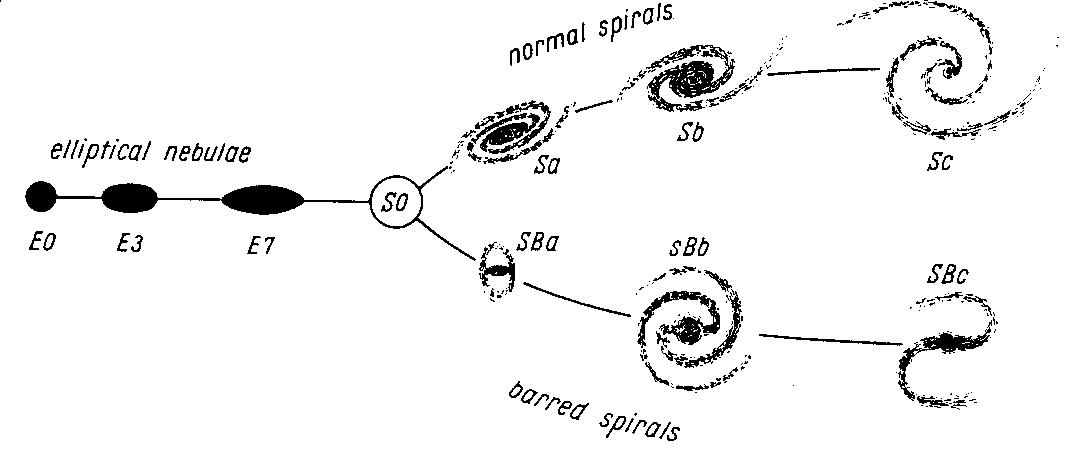
\includegraphics[width=\textwidth]{introduction/hubble.jpeg}}
\caption[The Hubble sequence for morphological classification of galaxies]{The Hubble sequence of galaxy morphology shown on his famous `tuning fork diagram' as published in \cite{hubble36}.}
\label{fig:hubble}
\end{figure}

However, the structure alone is not enough to describe a galaxy's evolution. The magnitude (used as a proxy for stellar mass), star formation rate (SFR), metallicity (Z) and environment are all crucial to describing a galaxy's current state. By studying these galaxy properties, insight into the processes which govern galaxy evolution can be gained.

Large scale surveys of galaxies have firstly revealed a bimodality in the optical colour-magnitude diagram (CMD) of galaxies finding two distinct populations (see Figure~\ref{fig:cmdbaldry}); one at relatively low mass, with blue optical colours and another at relatively high mass, with red optical colours \citep{Baldry04, Baldry06, Willmer06, ball08, Brammer09}. These populations were dubbed the `blue cloud' and `red sequence' respectively \citep{Chester64, bower92, Driver06, Faber07}.  The sparsely populated colour space between these two populations was dubbed the  `green valley'.

\begin{figure}[t]
\centering{
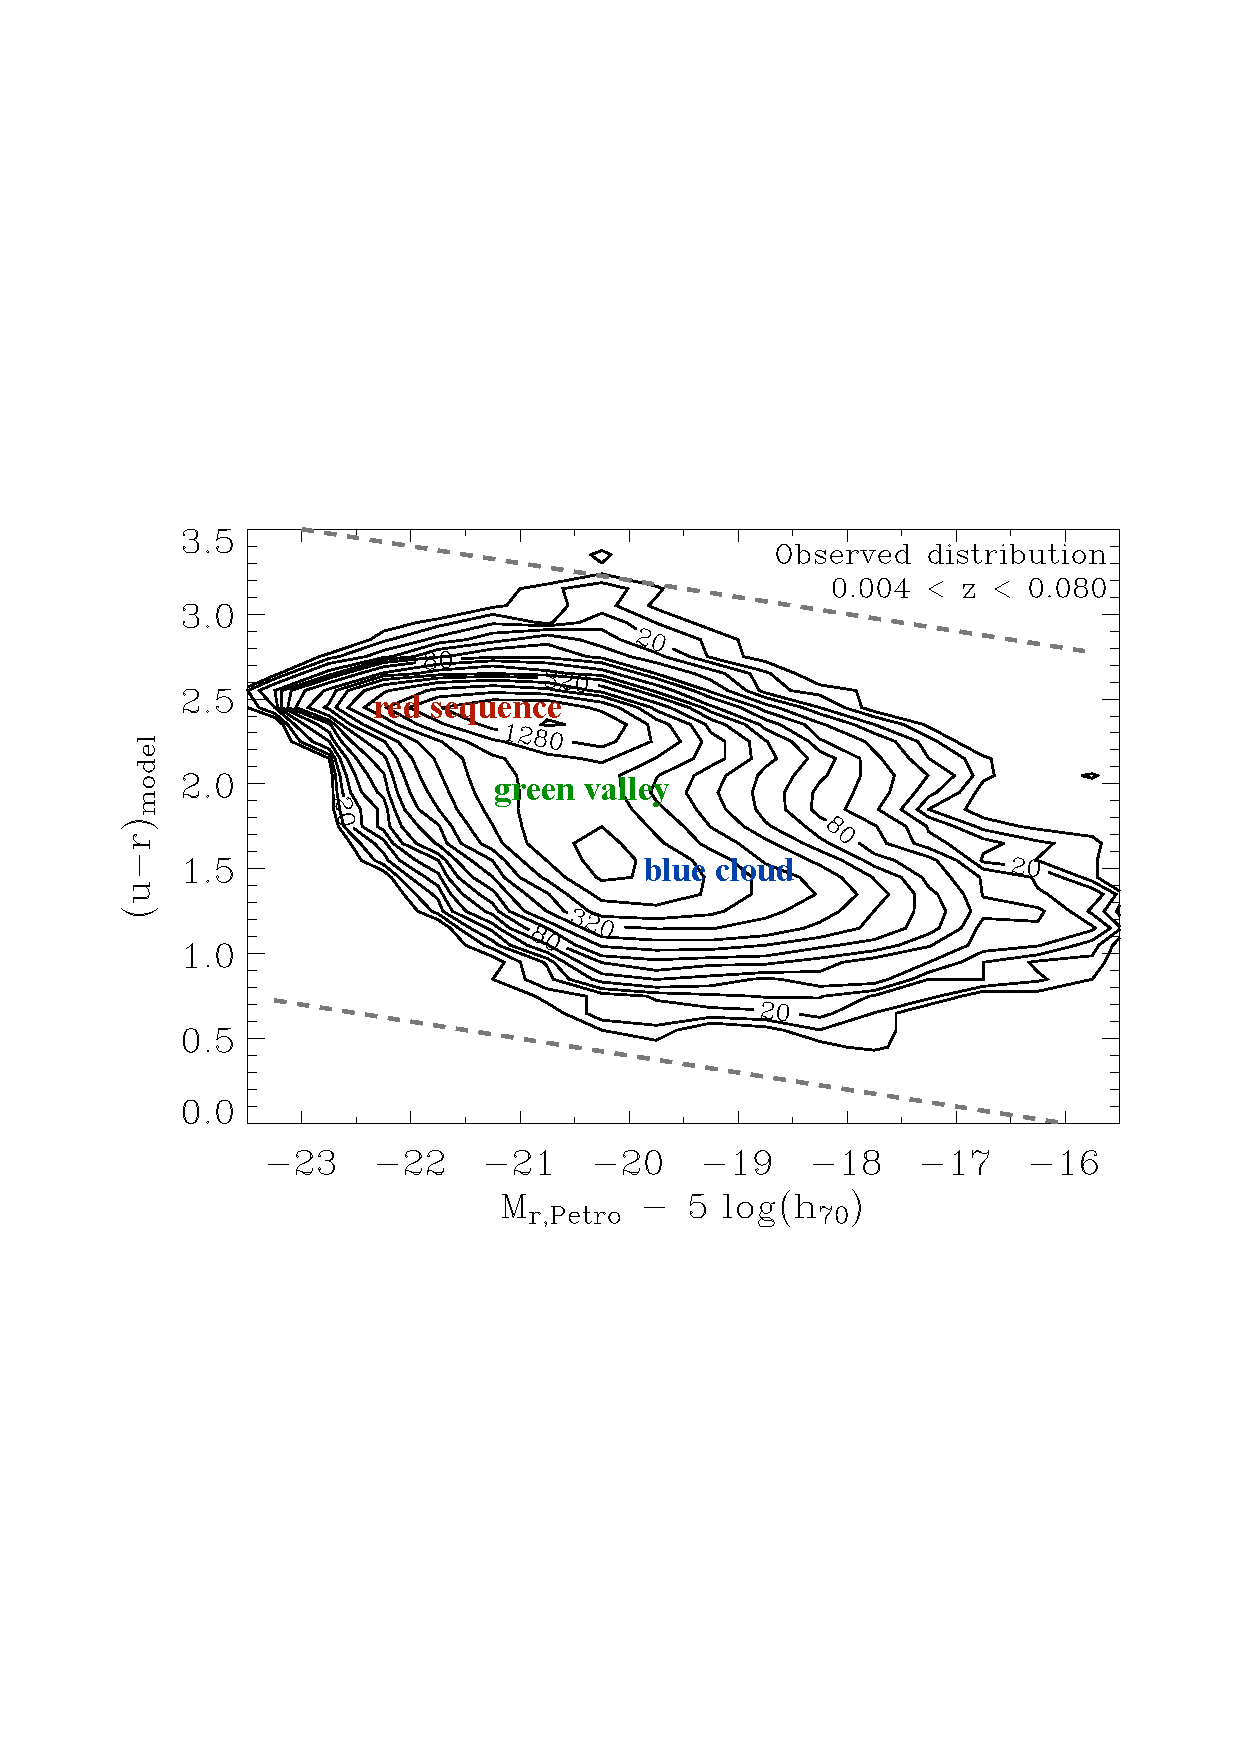
\includegraphics[width=\textwidth]{introduction/cmd.pdf}}
\caption[Galaxy Colour Magnitude Diagram from \cite{Baldry04}]{The galaxy colour magnitude diagram as observed by \cite{Baldry04}. The figure has been adapted from Figure 1 in \citeauthor{Baldry04} and annotated to show the locations of the red sequence and blue cloud. A lower magnitude corresponds to a higher mass and a large $u-r$ value corresponds to a redder colour.}
\label{fig:cmdbaldry}
\end{figure}


The majority of disc galaxies were found in the blue cloud and the majority of ellipticals on the red sequence, with colour often used as a proxy for morphology. The Galaxy Zoo project \citep{lintott08, Lintott11}, which produced morphological classifications for a million galaxies, helped to confirm that this colour bimodality is not entirely morphology driven \citep{Strat01, Salim07, Sch07, CHV08, Bamford09, Skibba09}, detecting larger numbers of spiral galaxies in the red sequence \citep{masters10c} and elliptical galaxies in the blue cloud \citep{Sch09} than had previously been detected.

Secondly large galaxy surveys revealed that star forming galaxies are also observed to lie on a well defined `star forming sequence' (SFS) in the stellar mass vs. star formation rate (SFR) plane \citep{brinchmann04, Salim07, Daddi07}. The majority of blue cloud galaxies are found to lie on this SFS with the majority of the red sequence lying well below it with very low SFRs. The intermediate colours of the green valley have therefore been interpreted as evidence of recent suppression of star formation \citep[SF;][]{Salim07}. This suppression of SF and subsequent transition of a galaxy from blue cloud to red sequence must therefore also be intrinsically tied with a possible (but not necessary) change in morphology from a disc galaxy to an elliptical galaxy.

A driver of this morphological change is thought to be the density of the galaxy environment. Due to the hierarchical nature of structure formation in $\Lambda$-CDM, galaxies are often found huddled together in groups \citep{zwicky38, zwicky52, abell58}, all sharing one large dark matter halo (groups with 100 or more galaxies are referred to as clusters \citealt{bower04}). Conversely some galaxies are found isolated from others in less dense environments (often referred to as the field), either because they are fossil groups \citep[where all members have eventually merged][]{ponman94, jones00, jones03} or have truly been isolated for their entire lifetimes. This environmental density is found to be correlated not only with morphology \citep[][and see Figure~\ref{fig:dressler}]{dressler80, smail97, poggianti99, postman05, Bamford09}, but also colour \citep{butcher78, pimbblet02}, quenched galaxy fraction \citep{kauffmann03, Baldry06, peng12, darvish16} and SFR \citep{gomez03} suggesting that the environment may drive this transition from blue cloud to red sequence. 

\begin{figure}[t]
\centering{
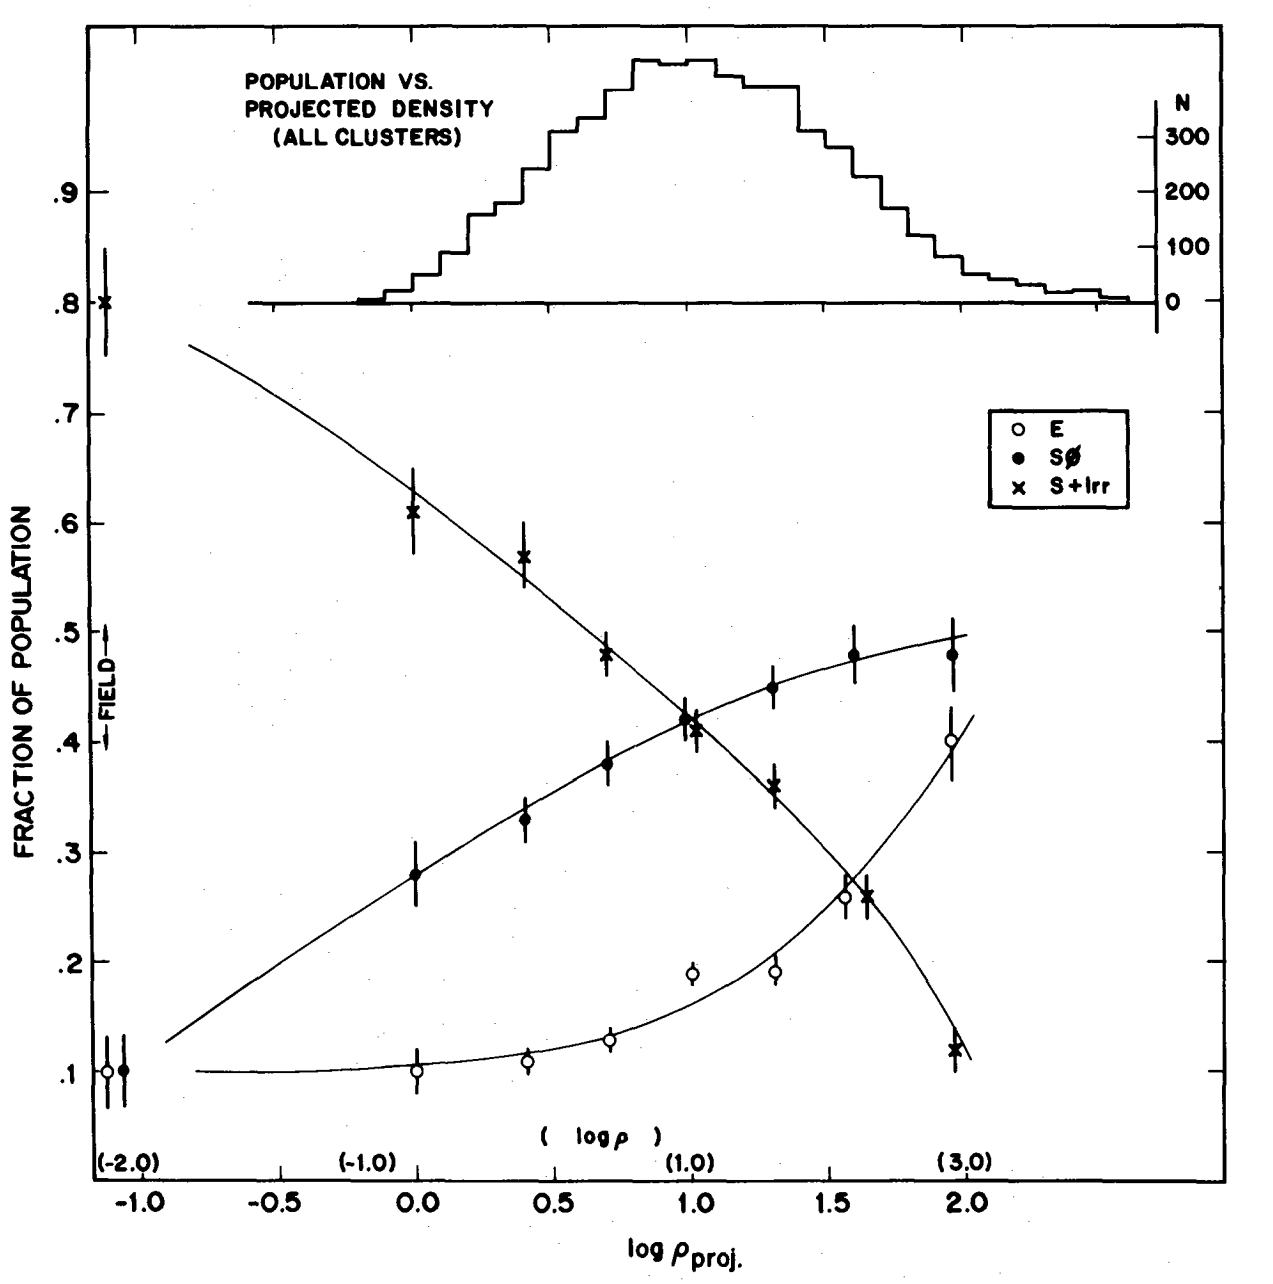
\includegraphics[width=0.8\textwidth]{introduction/dressler.png}}
\caption[Morphology Density relation from Figure 4 of \cite{dressler80}]{The morphology-density relation from Figure 4 of \cite{dressler80} showing how the fraction of ellipticals (E) increases with increasing environmental density and the fraction of spirals (S + Irr) decreases.}
\label{fig:dressler}
\end{figure}

Green valley galaxies have therefore long been thought of as the `crossroads' of galaxy evolution, a transition population between the two main galactic stages of the star forming blue cloud and the `dead' red sequence \citep{Bell04, Wyder07, Schim07, Martin07, Faber07, Mendez11, Gonc12, schawinski14, Pan14}. This transition is theorised to occur on rapid timescales, otherwise there would be an accumulation of galaxies residing in the green valley, rather than an accumulation in the red sequence as is observed \citep{Arnouts07, Martin07}.

I will refer to this suppression of a galaxy's SFR as \emph{quenching} and processes which can cause this suppression as \emph{quenching mechanisms}. By studying these galaxies which are quenching, having just left the SFS sequence, the mechanisms governing galaxy evolution, including both the suppression of SF and the possible transformation of galaxy structure, can be probed. 

\section{Possible quenching mechanisms}\label{sec:quenchmech}

There are many theorised mechanisms which can cause quenching. They are often referred to as either \emph{internal} mechanisms (caused by the galaxy's \emph{nature}) or \emph{external} mechanisms (caused by the way the galaxy is \emph{nurtured}). The properties of a galaxy and its environment are often thought to control which mechanisms will affect a galaxy throughout its lifetime and subsequently affect the morphology. 

%There have been many previous theories for the initial triggers of these quenching mechanisms, including negative feedback from AGN \citep{diMatteo05, Martin07, Nandra07, Sch07}, mergers \citep{Darg10a, Cheung12, Barro13}, supernovae winds \citep{MFB12}, cluster interactions \citep{Coil08, Mendez11, Fang13} and secular evolution \citep{masters10c, masters11a, Mendez11}. By investigating the \emph{amount} of quenching that has occurred in the blue cloud, green valley and red sequence; and by comparing the amount across these three populations, I can apply some constraints to these theories. 
\subsection{Internal Quenching Mechanisms}\label{sec:intquench}

\subsubsection{AGN feedback as a quenching mechanism}\label{sec:agnquench}

An active galactic nucleus (AGN) is an actively growing supermassive black hole in the centre of a galaxy. Feedback from an AGN is one of the most investigated mechanisms of quenching due to the tight correlations between properties of galaxies and their black holes \citep{magorrian98, marconi03, haringrix04}. This implies that the formation energy of the black hole and galaxy are coupled, leading to a co-evolution. This suggests that changes in the SFR and structure of a galaxy could also be tied to  black hole activity. 

The output of energetic material and radiation generated by the accretion onto the black hole is theorised to either heat or expel gas needed for SF in a galaxy, causing a quench. AGN feedback was first suggested as a mechanism for regulating star formation due to the results of simulations wherein galaxies could grow to unrealistic stellar masses \citep{silk98, Bower06, Croton06, somerville08}. Without a prescription for the effects of AGN feedback, the shape of the galaxy luminosity function could therefore not be matched at the high luminosity end \citep{baugh98, baugh05, kauffmann99a, kauffmann99b, somerville01, kitzbichler06}. A similar problem was also encountered at the low end of the luminosity function, which was rectified by the inclusion of the effects of supernova wind feedback \citep{dekel86, powell11}. This is illustrated in Figure~\ref{fig:lumfuncpic} taken from \cite{silk12}. 

\begin{figure}[t]
\centering{
\includegraphics[width=0.8\textwidth]{introduction/silk_mamon_LF.pdf}}
\caption[Illustration of the mismatch between theoretical and observed luminosity function from Silk \& Mamon (2012)]{Cartoon of the role of feedback in modifying the observed luminosity function of galaxies with respect to theoretical predictions. Supernova winds are thought to be responsible at the low mass end, with AGN feedback responsible at the high mass end. Figure 1 in \cite{silk12}.}
\label{fig:lumfuncpic}
\end{figure}

Indirect observational evidence has now been found for both positive and negative feedback in various systems (see the comprehensive review from \citealt{fabian12}). The strongest of which is the indirect evidence that the largest fraction of AGN are found in the green valley \citep{cowie08, Hickox09, schawinski10a}, suggesting a link between AGN activity and the process which moves a galaxy from the blue cloud to the red sequence. However, concrete statistical evidence for the effect of AGN feedback on the host galaxy population has so far been elusive.


\subsubsection{Mass quenching}\label{sec:massquench}
Mass quenching is the process by which a galaxy, independent of its environment, uses up its available gas for star formation via the Kennicutt-Schmidt law \citep{schmidt59, kennicutt98} and consequently grows in mass. As it does so there is less gas available for SF, and so in effect quenches itself \citep{peng12}. This is thought to be the dominant mechanism for isolated galaxies in the field \citep{kormendy04}. However, it is also thought that as a galaxy infalls in to a group or cluster over long timescales, gas reservoirs can be depleted via this mass quenching process \citep{peng12}.
 
\subsubsection{Morphological quenching}\label{sec:moprhquench}
Morphological quenching (or `secular' quenching, referring to slow, non-violent processes) is the process by which the internal structure of a galaxy can have a negative impact on its own SFR\footnote{Essentially shooting itself in the foot.}. This is theorised to occur in galaxies hosting bars; the bar funnels gas to the centre of the galaxy \citep{athanassoula92a} where it is exhausted by star formation effectively quenching the galaxy \citep{zurita04, sheth05}. This process is thought to be responsible for large numbers of red spirals and supported by observations of increasing bar fraction with red colours \citep{masters11a}. 

This process is also theorised to be caused by bulges \citep{bluck14} whereby the large gravitational potential of the bulge prevents the disc from collapsing and forming stars \citep{Fang13}. Recent observational evidence from \citep{hart16} also suggests that spiral structure can also cause morphological quenching. \citeauthor{hart16} propose that many armed spiral structures can trigger galaxy wide starbursts thereby rapidly using up gas for future star formation; similarly two armed spirals are observed with redder colours, suggesting that this spiral phase is much longer lived and may funnel gas into the centre of the galaxy to be exhausted in star formation over longer timescales.  
  
\subsection{External Quenching Mechanisms}\label{sec:extquench}
  
\subsubsection{Mergers as a quenching mechanism}\label{sec:mergersquench}

Major mergers have been intrinsically linked to the formation of elliptical galaxies since \citet{toomre72} showed this was possible with a simulation of the merger of two equal mass disc galaxies. Since $\Lambda$-CDM relies on the idea of hierarchical structure formation through the merger of dark matter halos for its description of galaxy formation, it also follows that galaxy evolution should be further influenced by mergers. 

The hypothesis is as follows; when two galaxies merge, the influx of cold gas funnelled by the forces in the interaction often results in energetic starbursts \citep{mihos94, mihos96, hopkins06d, hopkins08a, hopkins08b, snyder11, hayward14, sparre16}, which can exhaust the gas required for star formation, effectively quenching the post-merger remnant. This remnant galaxy will also have formed a dynamically hot bulge through the dissipation of angular momentum in the merger \citep{toomre77, walker96, kormendy04, hopkins11c, martig12}. The mass ratio of the two galaxies merging is thought to effect the size of the bulge that is formed in the remnant \citep{cox08, hopkins09c, tonini16}, with the most massive major mergers with a 1:1 mass ratio producing fully elliptical galaxies \citep{toomre72, barnes96, mihos96, kauffmann96, pontzen16}.

Such a scenario is also intrinsically linked to the triggering of an AGN \citep{sanders88, dimatteo05, hopkins09a, treister12} and many studies have focussed on investigating the growth of black holes due to mergers \citep[e.g.][]{veilleux02, bellovary13, ellison13, medling15, gabor16}. Simulations of mergers with AGN have lead many to believe that a merger which triggered both a starburst and an AGN can quench a galaxy in extremely rapid timescales \citep{springel05b, bell06}. Recent simulations have also suggested that feedback from the triggered AGN (see Section \ref{sec:agnquench}) is necessary to fully remove (or heat) all the available gas, otherwise the SFR will recover back to the SFS post-merger \citep{pontzen16, sparre16}. 

\subsubsection{Environment driven quenching}\label{sec:envquench}

The environment of a galaxy has long been considered a key  \emph{nurturing} aspect of galaxy evolution. Correlations of galaxy morphology \citep{dressler80, smail97, poggianti99, postman05, Bamford09}, colour \citep{butcher78, pimbblet02} and the quenched galaxy fraction \citep{kauffmann03, Baldry06, peng12, darvish16} with the environmental density all suggest that the environment is in some way responsible for the build up of the red sequence through quenching. 

The proposed quenching mechanisms under the umbrella of environmental quenching are numerous and varied. Together with the typical gravitational galaxy-galaxy interactions \citep{moore96} expected to be more frequent in a dense environment, environmental quenching also includes hydrodynamic interactions occurring between the cold inter stellar medium (ISM) of the in-falling galaxy and the hot intergalactic medium (IGM) of the group or cluster. Such hydrodynamic interactions include ram pressure stripping \citep{gunngott72}, viscous stripping \citep{nulsen82}, and thermal evaporation \citep[a rapid rise in temperature of the ISM due to contact with the IGM;][]{cowie77}. Another such process is starvation \citep{larson80} which can remove the outer galaxy halo cutting off the star formation gas supply to a galaxy. Preprocessing occurs when all of the above mechanisms take place in a group of galaxies which then merges with a larger group or cluster \citep{dressler04}. 

The most likely candidate (and therefore the most studied) mechanism for the cause of the environmental density-morphology and SFR relations is ram pressure stripping \citep[RPS;][]{abadi99, poggianti99}. However, there has been mounting evidence that RPS may not be as effective as a quenching mechanism as first thought \citep{emerick16, fillingham16}, therefore investigations of other environmentally driven quenching mechanisms are having a recent resurgence \citep[e.g.][]{bialas15, peng15, smith15b, hahn16, maier16, paccagnella16, roberts16, vandevoort16}. 

\section{Using star formation histories to investigate quenching}\label{sec:invquench}

% previous work
% using SFHs
% the benefits of SPSs

In order to understand how a galaxy is quenched, the star formation history (SFH) is often modelled, i.e. how galaxy stellar populations change with time. This approach requires the inference of the global SFH of a galaxy from a its current stellar population. While in nearby galaxies it is possible to observe resolved stellar populations with the Hubble Space Telescope (HST) to pinpoint the main sequence turn off (an indicator of the age of a stellar population) on the Hertzsprung Russel diagram,this is not possible in more distant galaxies. Instead, reliance is placed upon the correlation between the integrated total light of a galaxy and its SFH \citep{searle73}. Many studies have employed this technique using either photometric broadband colours or spectral data as indicators of the integrated SFH \citep[for example][]{deJong96, madau98, kauffmann03, dressler04, macarthur04, Martin07, perez11, sanchez11}. However, this technique is sensitive to the degeneracies between age and metallicity \citep{worthey94} and the effects of dust \citep{ganda09, pastrav13} on the integrated light. 

The turn of the millennium therefore saw the development of full spectral energy density (SED) fitting codes to infer the SFH (without having to make any prior assumptions on its form) such as \textsc{moped} \citep{heavens00}, \textsc{starlight} \citep{cidfernandes05}, \textsc{vespa} \citep{tojeiro07}, and more recently \textsc{firefly} \citep{wilkinson15}. In the absence of spectral data however, broadband colours are still effective at inferring the global SFHs of galaxies, especially when wavebands across the spectrum, such as ultra-violet, optical and infrared colours, are used simultaneously \citep{madau98}. 

This method is achieved by modelling the observed spectrum of a galaxy using a combination of spectra of simple stellar populations (SSP) at various ages. SSPs assume stars are coeval and form with the same metallicity and comprehensive knowledge of stellar evolutionary tracks and initial mass functions \citep[IMF;][]{salpeter55, chabrier03} are therefore needed to calculate the spectrum of a SSP at a given age \citep{chen10, kriek10}. Luckily, some astronomers have made the study of these SSPs their life's work \citep[for example]{BC03, Maraston05, vazquez05, CGW09}, therefore once an IMF and a SFH function have been assumed, the SED of a model galaxy can be predicted at any point in its history \citep{chen10}. Whilst the choice of an IMF and metallicity of a SSP will affect the output SED \citep{CGW09, kriek10}, the choice of the functional form of the SFH will have the greatest impact. 

Many possible forms for global galaxy SFHs have been assumed in previous studies, including an exponential decline \citep{tinsley72, gavazzi02, weiner06, Martin07, noeske07, kriek10,  schawinski14, hart16}, the extended (or delayed) exponential model \citep{gavazzi02, oemler13, simha14}, a Gaussian distribution \citep{feuillet16} or a log normal distribution \citep{gladders13, abramson16}. These models are by no means a perfect description of a galaxy's SFH \citep{lee10, boquien14, smith15}, as they generalise the localised bursts of SF across a galaxy's lifetime into a global SFH, but they still allow some insight to be gained on the complex processes responsible for the SFHs seen across the galaxy population. 

\section{Data}\label{sec:data}

In the following section I describe the data sources for the colours and morphologies used throughout this study for the galaxy sample described in Section~\ref{sec:defsample}

\subsection{Sloan Digital Sky Survey}\label{sec:sdssintro}

The Sloan Digital Sky Survey (SDSS; \citealt{York00}) Data Release 8 \citep{Aihara11}, provides publicly available optical magnitudes across $5$ broadband filters, $ugriz$ for over 1 million galaxies in their `main galaxy' sample. Here I utilise the Petrosian magnitudes, {\tt petroMag}, values for the $u$ ($3,543\rm{\AA}$) and $r$ ($6,231\rm{\AA}$) wavebands provided by the SDSS pipeline. Spectral data is available for a significant proportion of the SDSS main galaxy sample but the spectral fibre is a set size. Therefore across a population of galaxies the fibre will cover varying amounts of galaxies at different distances and of different sizes. Therefore the usual spectral star formation indicators cannot be utilised in this study as they will not provide an estimate of the total SFR of a galaxy. 

Magnitudes are corrected for galactic extinction \citep{Oh11} by applying the \citet{Cardelli89} law, giving a typical correction of $u-r \sim 0.05$. K-corrections are also adopted to $z=0.0$ and absolute magnitudes obtained from the NYU-VAGC \citep{Blanton05, padmanabhan08, blanton07}, giving a typical $u-r$ correction of $\sim 0.15$ mag. The change in the $u-r$ colour due to both corrections therefore ranges from $\Delta u-r \sim 0.2$ at low redshift, increasing up to $\Delta u-r \sim 1.0$ at $z \sim 0.25$, which is consistent with the expected k-corrections shown in Figure 15 of \citet{blanton07}. These corrections were calculated by \citet{Bamford09} for a subset of galaxies in the SDSS survey. These corrections are a crucial aspect of this work since a $\Delta u-r \sim 1.0$ can cause a galaxy to change whether it is class as blue cloud, green valley or red sequence.

Star formation rates and stellar masses, where available, were obtained from the MPA-JHU catalog \citep{kauffmann03, brinchmann04}. I used the average values, \textsc{avg sfr} and \textsc{avg mass}, which are corrected for aperture effects and extinction.

\subsection{Galaxy Evolution Explorer}\label{sec:galexintro}

The Galaxy Evolution Explorer (GALEX; \citealt{Martin05}) images galaxies simultaneously in two broadband filters: both the far ultra-violet (FUV) with an effective wavelength of $1,516\rm{\AA}$ and in the NUV with an effective wavelength of $2,267\rm{\AA}$. GALEX sources were matched with a search radius of $1''$ to the SDSS data in right ascension and declination. The {\tt auto} magnitudes provided by the GALEX pipeline are used in this study (for a discussion of aperture bias between different surveys see \citealt{hill11}). All magnitudes are k-corrected and extinction corrected as described in Section~\ref{sec:sdssintro}.

\subsection{Galaxy Zoo}\label{sec:GZ}

Galaxy Zoo (GZ) is a citizen science project enlisting the help of thousands of members of the public to voluntarily classify SDSS galaxy images online\footnote{\url{http://galaxyzoo.org}}. The first version of GZ classified just under 1 million SDSS galaxy images as either ellipticals, spirals or mergers within approximately 6 months of launch \citep{lintott08, Lintott11}. In the second version, GZ2 \citep{GZ2}, users were asked to make more detailed morphological classifications of $304, 022$ images from the SDSS DR8 (a subset of those classified in the first Galaxy Zoo; GZ1). These images were all classified by \emph{at least} 17 independent users, with the mean number of classifications standing at $\sim42$. GZ is now in its ninth year of classifying and its fifth incarnation, after classifying images from Hubble Space Telescope Legacy surveys in GZ:Hubble \citep{willett16} and the CANDELS survey galaxies in GZ:CANDELS \citep{simmons16}. At the time of writing, images from the DeCALS\footnote{\url{http://legacysurvey.org/}} survey and Illustrius simulation \citep{vogelsberger14, genel14} are being classified by users. 

\begin{figure}
\centering{
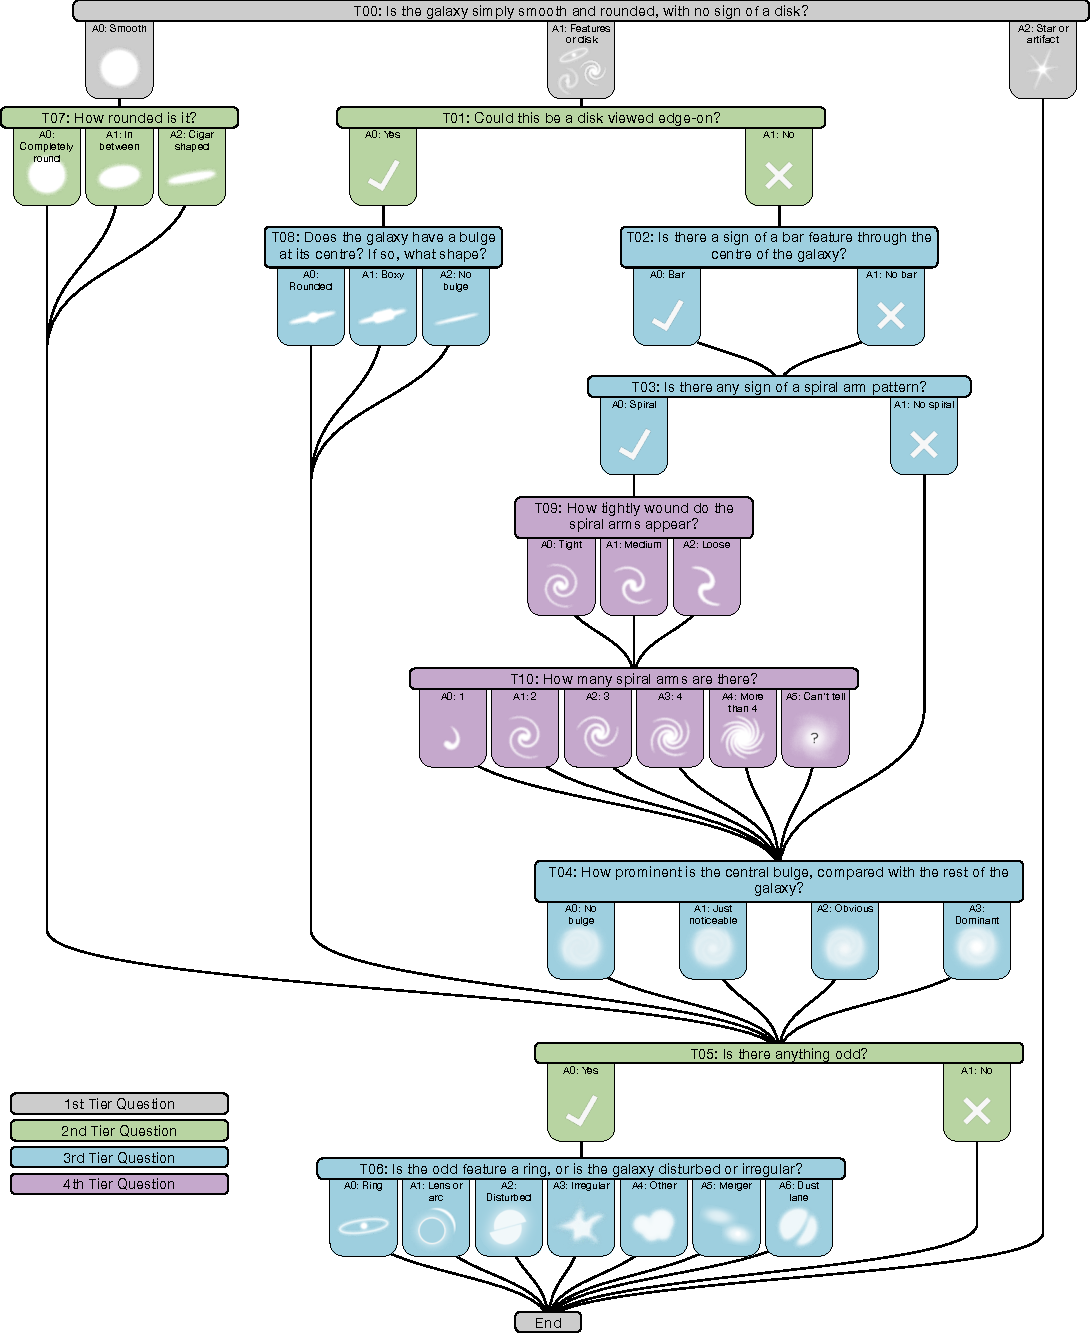
\includegraphics[width=\textwidth]{introduction/gz2_tree.pdf}}
\caption[GZ2 classification decision tree]{Flowchart of the classification tree for GZ2, beginning at the top with Task 0. Tasks are colour-coded by their relative depths in the decision tree with tasks in green, blue and purple respectively one, two or three steps below branching points in the decision tree.}
\label{fig:gztree}
\end{figure}

Since GZ2, all projects have collected classification data via a multi-step decision tree, shown in Figure~\ref{fig:gztree}.  Each individual step in a tree is a \emph{task}, which consists of a \emph{question} with a finite number of possible \emph{answers}. The selection of an answer is called the user's \emph{vote}. The first task of GZ2 asks users to choose whether a galaxy is mostly smooth, is featured and/or has a disc or is a star/artefact. Unlike other tasks further down the decision tree, every user who classifies a galaxy image will complete this task (others, such as whether the galaxy has a bar, is dependent on a user having first classified it as a featured galaxy). Therefore the most statistically robust classifications are available at this level.

% The Galaxy Zoo 2 (GZ2) project consists of $304, 022$ images from the SDSS DR8 (a subset of those classified in Galaxy Zoo 1; GZ1) all classified by \emph{at least} 17 independent users, with the mean number of classifications standing at $\sim42$. The GZ2 sample is more robust than the GZ1 sample and provides more detailed morphological classifications, including features such as bars, the number of spiral arms and the ellipticity of smooth galaxies. It is for these reasons I use the GZ2 sample, as opposed to the GZ1, allowing for further investigation of specific galaxy classes in the future. 

The classifications from users produces a vote fraction for each galaxy; for example if 80 of 100 people thought a galaxy was featured and/or had a disc, whereas 20 out of 100 people thought the same galaxy was mostly smooth (i.e. elliptical), that galaxy would have raw vote fractions $p_{sd} = 0.8$ and $p_{d} = 0.2$. In this example this galaxy would be included in the \emph{`clean'} disc sample ($p_d \geq 0.8$) according to \cite{GZ2} and would be considered a late-type galaxy. Similar vote fractions can be produced at each stage in the tree, such as $\{p_{\mathrm{bar}}, p_{\mathrm{no~bar}}\}$, $\{p_{\mathrm{spiral}}, p_{\mathrm{no~spiral}}\}$ and $\{p_{\mathrm{odd}}, p_{\mathrm{not~odd}}\}$. Selecting a sample of galaxies with a specific feature using these vote fractions becomes a trade off between purity and completeness. Since not every user will submit a response to a 2nd, 3rd or 4th tier question (see Figure~\ref{fig:gztree}), the number of classifiers recording a response must be considered, in order to reduce noise in cases where only a small number of people answered that task. 

For example imagine that a galaxy is classified by $40$ people, $38$ of whom say that the galaxy is mostly smooth in answer to the first question. However, $2$ people decide that the galaxy is featured and/or has a disc, both of whom subsequently respond to Task 2 to say that there is a sign of a bar in the same galaxy. This would give a $p_{\rm{bar}}=1$, despite the fact that the $p_s = 0.95$. This is an unlikely situation, but highlights the need for not only consideration of the number of respondents for a task but also the vote fractions of previous tasks when using a threshold to identify a subset of features. Appropriate values for these thresholds given the number of respondents are shown in Table~\ref{table:votes} (reproduced from Table 3 in \citealt{GZ2}) and are adopted where relevant throughout this study. 

\begin{table}
\centering
 \begin{tabular*}{\textwidth}{l@{\extracolsep{\fill}}lcc}
 \hline
\multicolumn{1}{l}{Task} &
\multicolumn{1}{l}{Previous task} &
\multicolumn{1}{c}{Vote fraction} &
\multicolumn{1}{c}{Vote fraction}
\\ 
\multicolumn{1}{l}{} &
\multicolumn{1}{l}{} &
\multicolumn{1}{c}{$N_{task}\geq10$} &
\multicolumn{1}{c}{$N_{task}\geq20$}
\\ 
\hline					
00                      & --        & --        & --        \\
01                      & 00        & 0.227     & 0.430     \\
02                      & 00,01     & 0.519     & 0.715     \\
03                      & 00,01     & 0.519     & 0.715     \\
04                      & 00,01     & 0.519     & 0.715     \\
05                      & --        & --        & --        \\
06                      & 05        & 0.263     & 0.469     \\
07                      & 00        & 0.223     & 0.420     \\
08                      & 00,01     & 0.326     & 0.602     \\
09                      & 00,01,03  & 0.402     & 0.619     \\
10                      & 00,01,03  & 0.402     & 0.619     \\
\hline
\end{tabular*}
\caption[Thresholds for selecting sub-samples of galaxies using GZ2 data]{Thresholds for determining well-sampled galaxies in GZ2. Thresholds depend on the number of respondents for a task, including the thresholds that should be applied to previous task(s) for both 10 and 20 respondents. As an example, to select galaxies that may or may not contain bars, cuts for $p_\mathrm{features/disk}>0.430$, $p_\mathrm{not~edgeon}>0.715$, and $N_\mathrm{not~edgeon}\geq20$ should be applied. No thresholds are given for Tasks 01 and 06, since these are answered for every classification in GZ2. The task numbers are those defined in Figure~\ref{fig:gztree}.}
\label{table:votes}
\end{table}

All previous Galaxy Zoo projects have also incorporated extensive analysis of volunteer classifications to measure classification accuracy and bias. A weighting is computed for each user based on their classification history and agreement with the crowd in order to produce debiased vote fractions (for a detailed description of debiasing and consistency-based user weightings, see either Section 3 of \citealt{Lintott09} or Section 3 of \citealt{GZ2}). This produces highly accurate and robust detailed morphological classifications and is a significant statistical improvement over efforts completed using only a small number of expert classifiers \citep{schawinski07, nair10b, ann15}. These classifications can now be used as machine learning training sets \citep{dieleman15} to improve future automated classifications of galaxies. 

The debiased GZ2 $p_d$ and $p_s$ vote fractions encompass the continuous spectrum of morphological features (as shown in Figure~\ref{fig:mosaic}), rather than a simple binary classification separating elliptical and disc galaxies (see Section~\ref{sec:bigpic}). These classifications allow each galaxy to be considered as a probabilistic object with both bulge and disc components. I utilise the debiased GZ2 vote fractions in this study to facilitate future work studying more detailed galaxy structures. 

\subsection{Defining the GZ2-GALEX main galaxy sample}\label{sec:defsample}

\begin{figure}
\centering{
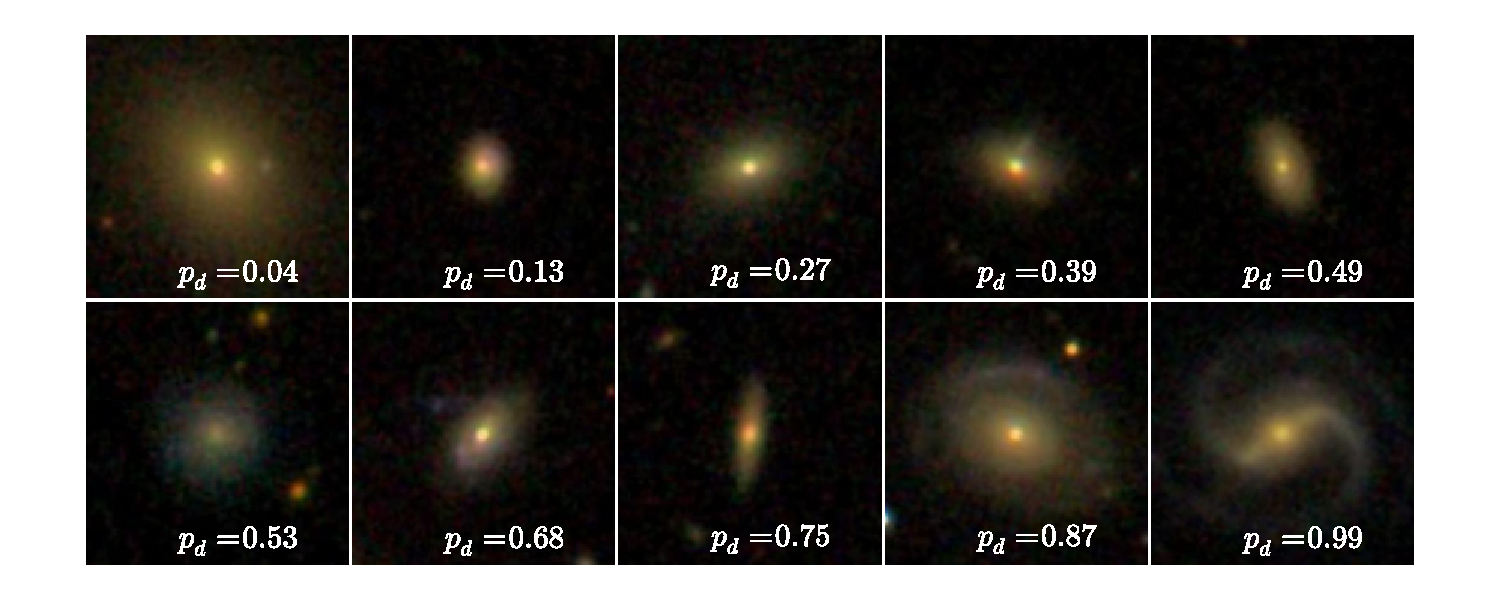
\includegraphics[width=\textwidth]{introduction/mosaic_disc_fraction_z_0-07_0-075.pdf}}
\caption[Example SDSS images with GZ2 vote fractions]{Randomly selected SDSS \emph{gri} composite images showing the continuous probabilistic nature of the Galaxy Zoo sample from a redshift range $0.070 < z < 0.075$. The debiased disc vote fraction for each galaxy is shown. The scale for each image is $0.099~\rm{arcsec/pixel}$.}
\label{fig:mosaic}
\end{figure}

\begin{figure}[t]
\centering{
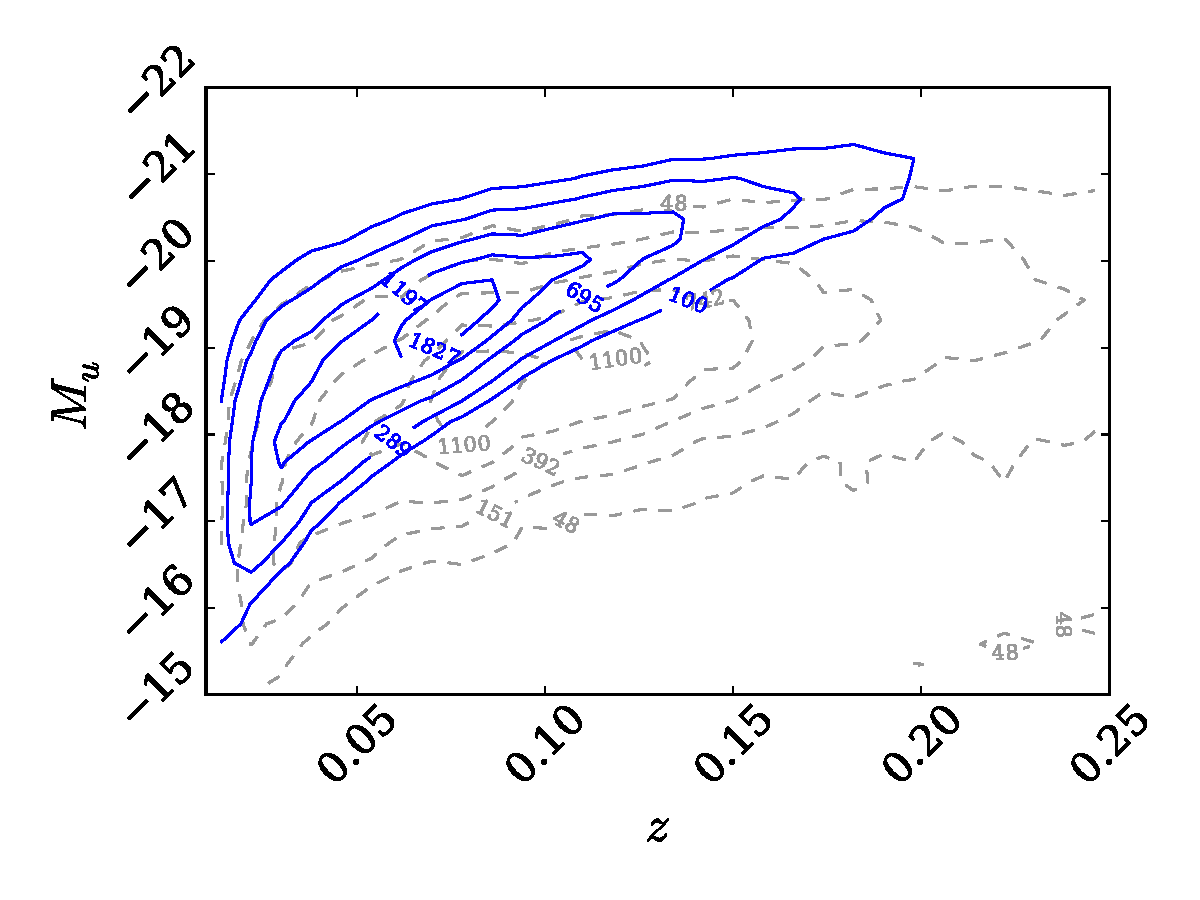
\includegraphics[width=\textwidth]{introduction/mag_redshift_completeness.pdf}}
\caption[GZ2-GALEX sample completeness]{Absolute $u$-band magnitude against redshift for the whole of SDSS (grey dashed lines) in comparison to the GZ2 subsample (blue solid lines). Typical Milky Way $L_*$ galaxies with $M_u \sim -20.5$ are still included in the GZ2 subsample out to the highest redshift.}
\label{complete}
\end{figure}


I require a sample of galaxies with optical and NUV photometry from SDSS and GALEX respectively, along with morphologies from GZ2 in order to study the morphological dependence of galaxy quenching histories. Starting with the $304,022$ SDSS galaxies in the GZ2 sample, objects considered to be stars or artefacts in Task 0 or merging pairs in Task 6 (using the thresholds defined in Table~\ref{table:votes}) were removed. Further to this, I required NUV photometry from the GALEX survey, within which $\sim42\%$ of the GZ2 sample galaxies were observed, giving a total sample size of $126, 316$ galaxies. This will be referred to as the \textsc{gz2-galex} sample. 

The completeness of the \textsc{gz2-galex} sample is shown in Figure~\ref{complete} with the $u$-band absolute magnitude against redshift, compared with the SDSS data set. Typical Milky Way $L_*$ galaxies with $M_u \sim -20.5$ are still included in the GZ2 subsample out to the highest redshift of $z \sim 0.25$; however dwarf and lower mass galaxies are only detected at the lowest redshifts.

Galaxy colours were not corrected for intrinsic dust attenuation. This is of particular consequence for disc galaxies, where attenuation increases with increasing inclination. \cite{Buat05} found the median value of the attenuation in the GALEX NUV passband to be $\sim 1$ mag. Similarly \cite{masters10a} found a total extinction from face-on to edge-on spirals of 0.7 and 0.5 mag for the SDSS $u$ and $r$ passbands and show spirals with $\log(a/b) > 0.7$ have signs of significant dust attenuation. For the \textsc{gz2-galex} sample I find $\sim29\%$ of discs (with $p_d > 0.5$) have $\log(a/b) > 0.7$, therefore we must be aware of possible biases in the results due to dust. 

I shall use the \textsc{gz2-galex} sample to probe how different quenching mechanisms cause galaxies of different morphologies and environments to transition from the SFS to quiescence. 


\section{Thesis Summary}\label{sec:thesissum}


This thesis proceeds as follows. In Chapter~\ref{chap:starpy} I describe the SFH model used to characterise the colours of quenching galaxies, along with the statistical methods used to determine the distribution of quenching histories in a population of galaxies. In Chapter~\ref{chap:morph} I apply this method across the red sequence, green valley and blue cloud and investigate the morphological dependence of quenching histories in these populations. Chapter~\ref{chap:agn} is split into two parts. In Section~\ref{sec:agnfeedback} I investigate the effect of AGN feedback on the quenching histories of a  population of AGN host galaxies. In Section~\ref{sec:intbulgeless} I investigate the proposed slow co-evolution of galaxies with their central black holes, by measuring the black hole masses of a sample of bulgeless galaxies, which have assumed merger free histories. In Chapter~\ref{chap:env} I return to investigating the quenching histories of galaxies, this time focussing on the effect of the group environment on satellite galaxies in comparison to centrals and those in the field. In Chapter~\ref{chap:discussion} I discuss how the implications of my results in the context of galaxy evolution and propose ideas for future work.

Where necessary I adopt the Planck 2015 cosmological results \citep{planck16} with $(\Omega_m, \Omega_{\lambda}, h) = (0.309 \pm 0.006, 0.691 \pm 0.006, 0.677 \pm 0.005)$. 

\chapter{STARPY: Bayesian inference of a galaxy's star formation history}

\emph{The work in the following chapter has been published in \citet{smethurst15}.}
\\

\section{Star Formation History Models}\label{qmod}

The quenched star formation history (SFH) of a galaxy can be simply modelled as an exponentially declining star formation rate (SFR) across cosmic time ($0 \leq t ~\rm{[Gyr]} \leq 13.8$) as:
\begin{equation}\label{sfh}
SFR =
\begin{cases}
I_{sfr}(t_q) & \text{if } t < t_q \\
I_{sfr}(t_q) \times exp{\left( \frac{-(t-t_{q})}{\tau}\right)} & \text{if } t > t_q 
\end{cases}
\end{equation}
where $t_{q}$ is the onset time of quenching, $\tau$ is the timescale over which the quenching occurs and $I_{sfr}$ is an initial constant star formation rate dependent on $t_q$.  A smaller $\tau$ value corresponds to a rapid quench, whereas a larger $\tau$ value corresponds to a slower quench. 

Here I assume that all galaxies formed at a time $t=0~\rm{Gyr}$ with an initial burst of star formation. The mass of this initial burst is controlled by the value of the $I_{sfr}$ which is set as the average specific SFR (sSFR) at the time of quenching $t_q$.  \citet{peng10} defined a relation (their equation 1) between the average sSFR and redshift (cosmic time, $t$) by fitting to measurements of the mean sSFR of blue star forming galaxies from SDSS, zCOSMOS and literature values at increasing redshifts \citep{Elbaz07, Daddi07}:
\begin{equation}
sSFR(m,t) = 2.5 \left( \frac{m}{10^{10} M_{\odot}} \right)^{-0.1} \left(\frac{t}{3.5 ~\rm{Gyr}}\right)^{-2.2} \rm{Gyr}^{-1}.
\end{equation}
Beyond $z \sim 2$ the characteristic SFR flattens and is roughly constant back to $z\sim6$. The cause for this change is not well understood but can be seen across similar observational data \citep{peng10, gonzalez10, bethermin12}. Motivated by these observations, the relation defined in \citet{peng10} is taken up to a cosmic time of $t=3~\rm{Gyr}~(z \sim 2.3)$ and prior to this a constant average SFR is assumed (see middle panel of Figure~\ref{sfr_mass_col}). At the point of quenching, $t_{q}$, the SFH models are defined to have an $I_{sfr}$ which lies on this relationship for the sSFR, for a galaxy with mass, $m = 10^{10.27} M_{\odot}$ (the mean mass of the \textsc{gz2-galex} sample; see left panel of Figure~\ref{sfr_mass_col}).

\begin{figure*}
\centering{
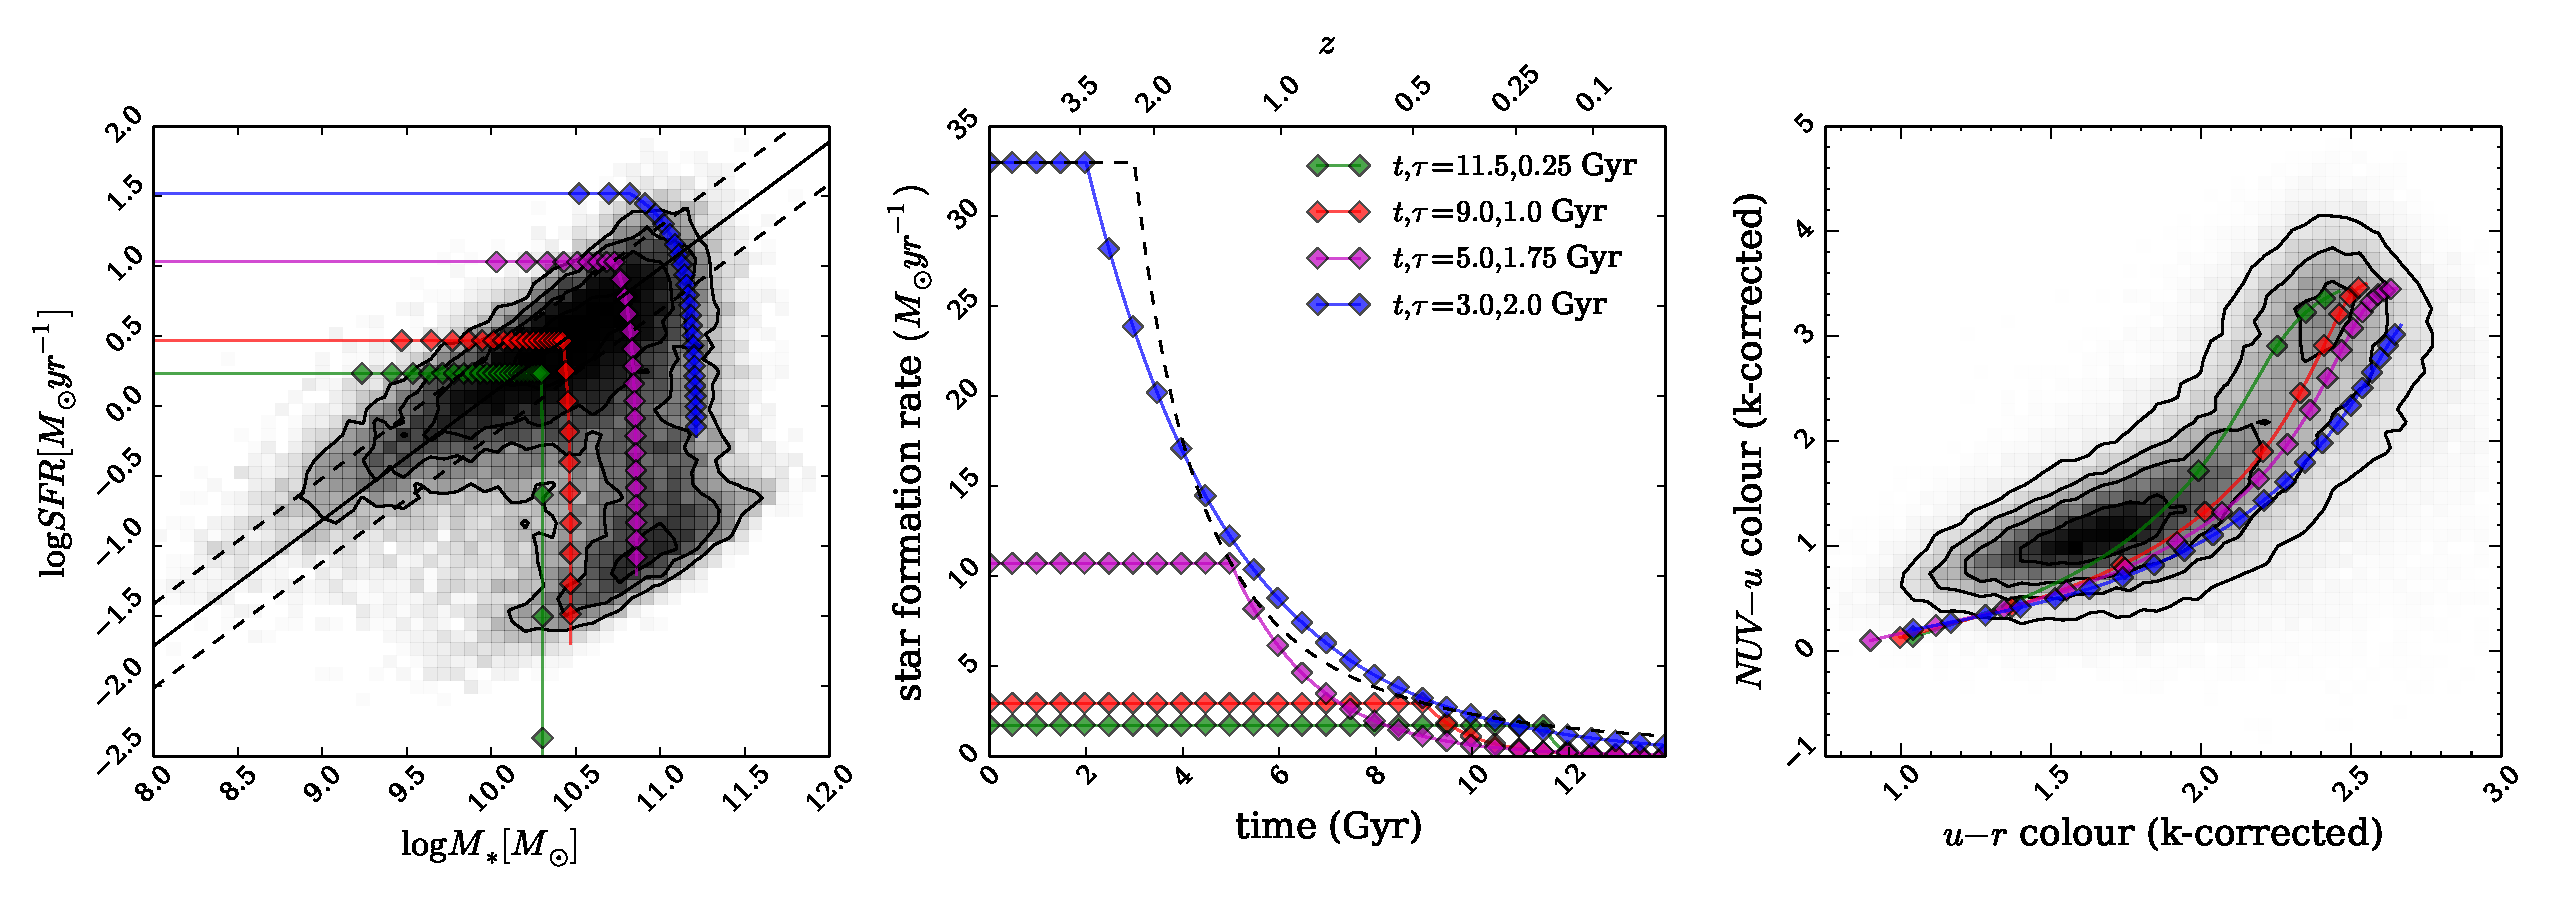
\includegraphics[width=\textwidth]{starpy/sfr_mass_colour_diagram.pdf}}
\caption[SFH models in observational planes]{Left panel: SFR-stellar mass plane for all 126,316 galaxies in the \textsc{gz2-galex} sample (shaded contours), with model galaxy trajectories shown by the coloured lines, with each point representing a time step of $0.5~\rm{Gyr}$.  The `main sequence' of star formation as defined by \citet{peng10} is shown by the solid line with $\pm1\sigma$ (dashed lines). Middle panel: The SFHs of the models are shown, where the SFR is initially constant before quenching at time $t_q$ and thereafter exponentially declining with a characteristic timescale $\tau$. The SFR at the point of quenching is set to be consistent with the typical SFR of a star-forming galaxy at the quenching time, $t_q$ (dashed curve; \citealt{peng10}). Right panel: The full range of models can reproduce the observed colour-colour properties of the sample; for clarity the figures show only 4 of the possible models explored in this study. Note that some of the model tracks produce colours redder than the apparent peak of the red sequence in the GZ2 subsample; however this is not the \emph{true} peak of the red sequence due to the necessity for NUV colours from GALEX.}
\label{sfr_mass_col}
\end{figure*}
  
Under these assumptions the average SFR of these models will result in a lower value than the relation defined in \citet{peng10} at all cosmic times as each galaxy only resides on the `main sequence' at the point of quenching. However galaxies cannot remain on the `main sequence' from early to late times throughout their entire lifetimes given the unphysical stellar masses and SFRs this would result in at the current epoch in the local Universe \citep{bethermin12, Heinis14}. If prescriptions for starbursts, mergers, AGN etc. were included in this model, the reproduction of the average SFR across cosmic time would improve; however I have chosen to first focus on the simplest possible model.

Once this evolutionary SFR is obtained, it is convolved with the \citet{BC03} population synthesis models to generate a model SED at each time step. The observed features of galaxy spectra can be modelled using simple stellar population techniques which sum the contributions of individual, coeval, equal-metallicity stars. The accuracy of these predictions depends on the completeness of the input stellar physics. Comprehensive knowledge is therefore required of (i) stellar evolutionary tracks and (ii) the initial mass function (IMF) to synthesise a stellar population accurately. 

These stellar population synthesis (SPS) models are an extremely well explored (and often debated) area of astrophysics \citep{Maraston05, Eminian08, CGW09, falkenberg09, Chen10, Kriek10, miner11, melbourne12}. In this work I have chosen to utilise the \citet{BC03} \emph{GALEXEV} SPS models, along with a Chabrier IMF \citep{chabrier03}, across a large wavelength range ($0.0091 < ~\lambda~\rm{[\mu m]}~ < 160 $) with solar metallically (m62 in the \citet{BC03} models; hereafter BC03), to allow a direct comparison with \citet{schawinski14}.


Fluxes from stars younger than $3~$Myr in the SPS model are suppressed to mimic the large optical depth of protostars embedded in dusty formation clouds (as in \citealt{schawinski14}).  Filter transmission curves are then applied to the fluxes to obtain AB magnitudes and ultimately colours.  For a particular galaxy at an observed redshift, $z$, I calculate the observed time, $t^{obs}$ for that galaxy using the standard cosmological conversion between redshift and time provided in the \textsc{astropy} {\em Python} module \citep{astropy13}. The predicted colours of the SFH models at the observed redshift of each individual galaxy can then be compared to the observed colours directly.

\begin{figure}
\centering{
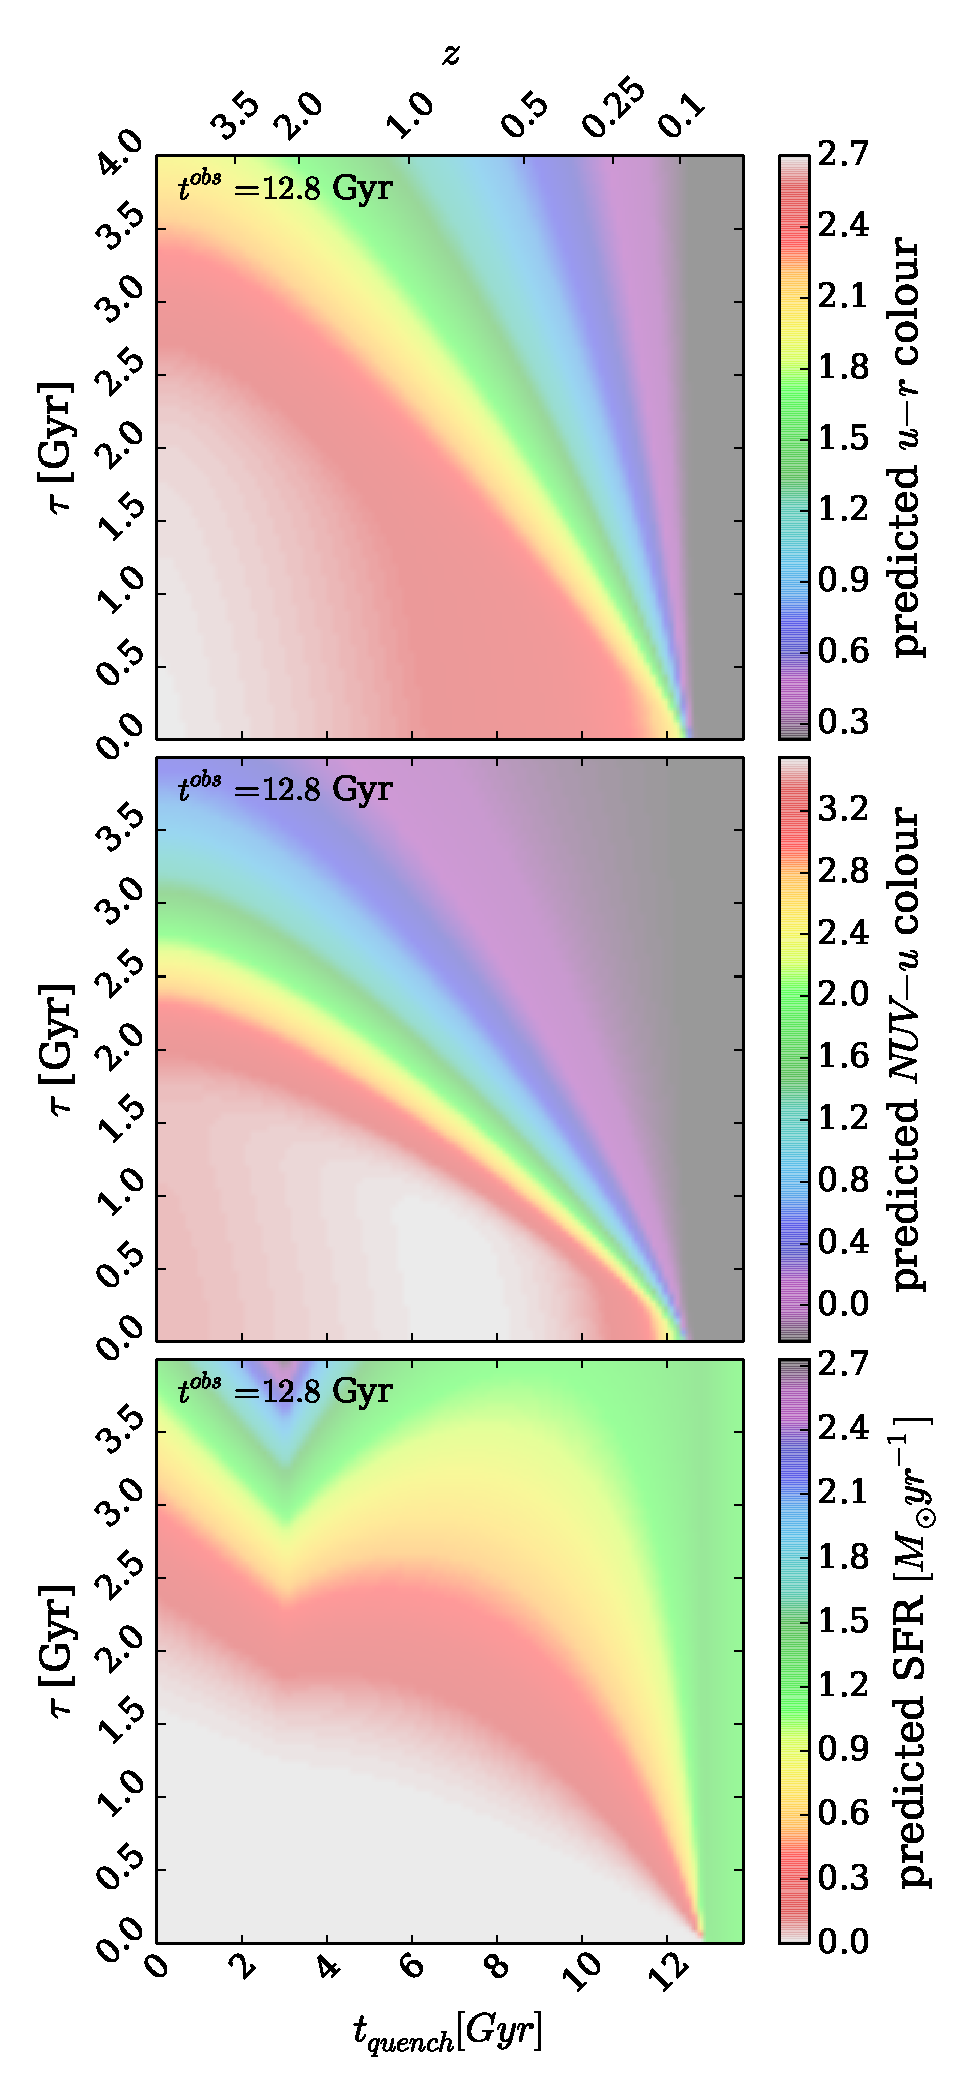
\includegraphics[height=0.75\textheight]{starpy/colours.pdf}}
\caption[Predicted colours and SFRs of quenching models]{Quenching timescale $\tau$ versus quenching onset time $t_q$ in all three panels for the quenched SFH models used in \starpy. Colour shadings show model predictions of the $u-r$ optical colour (top panel), $NUV-u$ colour (middle panel), and star formation rate (lower panel), at $t^{obs} = 12.8~\rm{Gyr}$, the mean observed redshift of the GZ2 sample (see Section \ref{qmod}). The combination of optical and NUV colours is a sensitive measure of the $\theta = [t_q, \tau]$ parameter space. Note that all models with $t > 12.8$ \rm{Gyr} are effectively un-quenched. The `kink' in the bottom panel is due to the assumption that the sSFR is constant prior to $t \sim 3~\rm{Gyr}$ ($z\sim 2.2$).}
\label{pred}
\end{figure}

Figure~\ref{pred} shows these predicted optical and NUV colours at a time of $t^{obs} = 12.8 ~\rm{Gyr}$ (the average observed time of the \textsc{gz2-galex} sample, $z \sim 0.076$) for the exponential SFH model. These predicted colours will be referred to as $d_{c,p}(t_{q}, \tau, t^{obs})$, where $c$=\{opt,NUV\} and $p$ = predicted. The SFR at a time of $t^{obs}=12.8~\rm{Gyr}$ is also shown in Figure~\ref{pred} to compare how this correlates with the predicted colours. The $u-r$ predicted colour shows an immediate correlation with the SFR, however the $NUV-u$ colour is more sensitive to the value of $\tau$ and so is ideal for tracing any recent star formation in a population . At small $\tau$ (rapid quenching timescales) the $NUV-u$ colour is insensitive to $t_{q}$, whereas at large $\tau$ (slow quenching timescales) the colour is very sensitive to $t_{q}$. Together the two colours are ideal for tracing the effects of $t_{q}$ and $\tau$ in a population. 

This model is not a fully hydrodynamical simulation, it is a simple model built in order to test our understanding of the evolution of galaxy populations. These models are therefore not expected to accurately determine the SFH of every galaxy in the \textsc{gz2-galex} sample, in particular galaxies which have not undergone any quenching. In this case the models described above can only attribute a constant star formation rate to these  unquenched galaxies. In reality, there are many possible forms of SFH that a galaxy can take, a few of which have been investigated in previous literature; starbursts \citep{Canalizo01}, a power law \citep{Glazebrook03}, single stellar populations \citep{Trager00, Sanchez06, Vazdekis10}, log-normal distributions \citep{abramson16} and metallicity enrichment \citep{deLucia14}. Incorporating these different SFHs along with prescriptions for mergers and a possible reinvigoration of star formation post quench (e.g. see recent work by \citealt{pontzen16}) into the SFH models is a possible future extension to this work once the results of this study are well enough understood to permit additional complexity to be added.

\section{Probabilistic Fitting Methods}\label{stats}

In order to achieve robust conclusions I conducted a Bayesian analysis \citep{Sivia, mackay03} of the predicted colours from the SFH models in comparison to the observed colours of the \textsc{gz2-galex} sample. This approach requires consideration of all possible combinations of $\theta \equiv (t_{q}, \tau)$. Assuming that all galaxies formed at $t=0~\rm{Gyr}$ with an initial burst of star formation, we can assume that the `age' of each galaxy in the GZ2 sample is equivalent to an observed time, $t^{obs}_{k}$. I then used this  `age' to calculate the predicted model colours at this cosmic time for a given combination of $\theta$: $d_{c,p}(\theta_k, t^{obs}_{k})$ for both optical and NUV $(c={opt,NUV})$ colours. The predicted model colours can now directly be compared with the observed \textsc{gz2-galex} sample colours, so that for a single galaxy $k$ with optical ($u-r$) colour, $d_{opt, k}$ and NUV ($NUV-u$) colour, $d_{NUV,k}$, the likelihood of a given model $P(d_{k}|\theta_k, t^{obs}_{k})$ is:


\begin{equation}\label{like}
\begin{split}
P(d_{k}|\theta_k, t^{obs}_{k}) = \frac{1}{\sqrt{2\pi\sigma_{opt, k}^2}}\frac{1}{\sqrt{2\pi\sigma_{NUV, k}^2}} \exp{\left[ - \frac{(d_{opt, k} - d_{opt, p}(\theta_k, t_{k}^{obs}))^2}{\sigma_{opt, k}^2} \right]} \\ \exp{\left[ - \frac{(d_{NUV, k} - d_{NUV, p}(\theta_k, t_{k}^{obs}))^2}{\sigma_{NUV, k}^2} \right]}.
\end{split}
\end{equation}


Here I have assumed that $P(d_{opt}|\theta_k, t^{obs}_{k})$ and $P(d_{NUV}|\theta_k, t^{obs}_{k})$ are independent of each other and that the errors on the observed colours are also independent. To obtain the probability of a combination of $\theta$ values \underline{given} the GZ2 data: $P(\theta_k|d_k, t^{obs})$, i.e. how likely is a single SFH model given the observed colours of a single GZ2 galaxy, I utilise Bayes' theorem:
 \begin{equation}\label{big}
P(\theta_k|d_k, t^{obs}) = \frac{P(d_k|\theta_k, t^{obs})P(\theta_k)}{\int P(d_k |\theta_k, t^{obs})P(\theta_k) d\theta_k}.
\end{equation}
I assume a flat prior on the model parameters so that:
\begin{equation}\label{prior}
P(\theta_k) =
\begin{cases}
1 & \text{if } 0 \leq t_q ~\rm{[Gyr]}~ \leq 13.8 ~  \text{ and } ~ 0 \leq \tau  ~\rm{[Gyr]}~ \leq 4\\
0 & \text{otherwise.} \\
\end{cases}
\end{equation}

\begin{figure}
\centering{
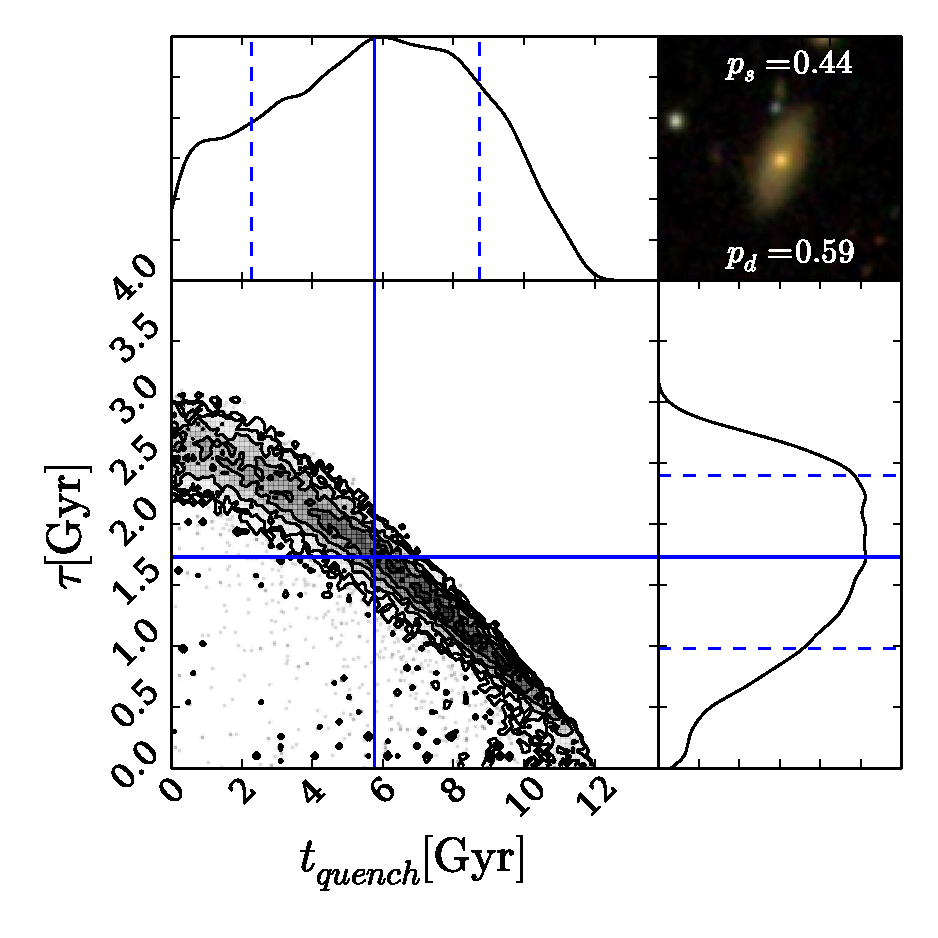
\includegraphics[width=0.9\textwidth]
{starpy/triangle_t_tau_red_s_1237655504035185152_40000_14_16_06_08_14.pdf}
\caption[Example \starpy ~output]{Example output from \starpy ~for a galaxy within the red sequence. The contours show the positions of the `walkers' in the Markov Chain (which are analogous to the areas of high probability) for the quenching models described by $\theta = [t_q, \tau]$. The histograms show the 1D projection along each axis. Solid (dashed) blue lines show the best fit parameters (with $\pm 1\sigma$) to the data. The postage stamp image from SDSS is shown in the top right along with the debiased vote fractions for smooth ($p_s$) and disc ($p_d$) from Galaxy Zoo 2.} }
\label{one_example}
\end{figure}

As the denominator of Equation~\ref{big} is a normalisation factor, comparison between likelihoods for two different SFH models (i.e., two different combinations of $\theta_k = [t_q, \tau]$) is equivalent to a comparison of the numerators. Markov Chain Monte Carlo (MCMC; \citealt{mackay03, emcee13, GW10}) provides a robust comparison of the likelihoods between $\theta$ values; here I choose \emph{emcee},\footnote{\url{emcee13.iel.fm/emcee/}} a Python implementation of an affine invariant ensemble sampler by \cite{emcee13}.

This method allows for a more efficient exploration of the parameter space by avoiding those areas with low likelihood. A large number of `walkers' are started at an initial position where the likelihood is calculated; from there they individually `jump' to a new area of parameter space. If the likelihood in this new area is greater (less) than the original position then the `walkers' accept (reject) this change in position. Any new position then influences the direction of the  `jumps' of other walkers. This is repeated for the defined number of steps after an initial `burn-in' phase. \emph{emcee} returns the positions of these `walkers', which are analogous to the regions of high probability in the model parameter space. 

The routine outlined above has been coded using the \emph{Python} programming language into a package named \starpy ~which has been made freely available to download\footnote{\url{github.com/zooniverse/starpy}}. An example output from this module for a single galaxy from the \textsc{gz2-galex} sample in the red sequence is shown in Figure~\ref{one_example}. 

\section{Testing STARPY}

\begin{figure}
\centering{
\includegraphics[width=\textwidth]{starpy/mosaic_test.jpg}}
\caption[Testing \starpy]{Results from \starpy ~for an array of synthesised galaxies with known, i.e. \underline{true}, $t_q$ and $\tau$ values (marked by the red lines) using the complete function to calculate the predicted colour of a proposed set of $\theta$ values in each MCMC iteration, assuming an error on the calculated known colours of $\sigma_{u-r} = 0.124$ and $\sigma_{NUV-u} = 0.215$ (the average errors on the GZ sample colours). I also assume that each synthesised galaxy has been observed at a redshift of $z=0$. In each case \starpy ~succeeds (50th percentile best fit parameters are shown by the blue lines) in locating the true parameter values within the degeneracies of the star formation history model.}
\label{test_mosaic}
\end{figure}

In order to test that \starpy ~can find the correct quenching model for a given observed colour, 25 synthesised galaxies were created with known SFHs (i.e. known values of $\theta = [t_q, \tau]$) from which optical and NUV colours were generated using the BC03 SPS models. These were input into \starpy ~ to test whether the known values of $\theta$ were reproduced, within error, for each of the 25 synthesised galaxies. Figure~\ref{test_mosaic} shows the results for each of these synthesised galaxies, with the known values of $\theta$ shown by the red lines. In some cases this red line does not coincide with the inferred best fit $\theta$ values shown by the blue lines, however in all cases the intersection of the red lines is within the sample contours; therefore \starpy succeeds in locating the true parameter values within the degeneracies of the SFH model. 

\section{Speeding up STARPY}\label{lookuptable}

\begin{figure*}
\centering{
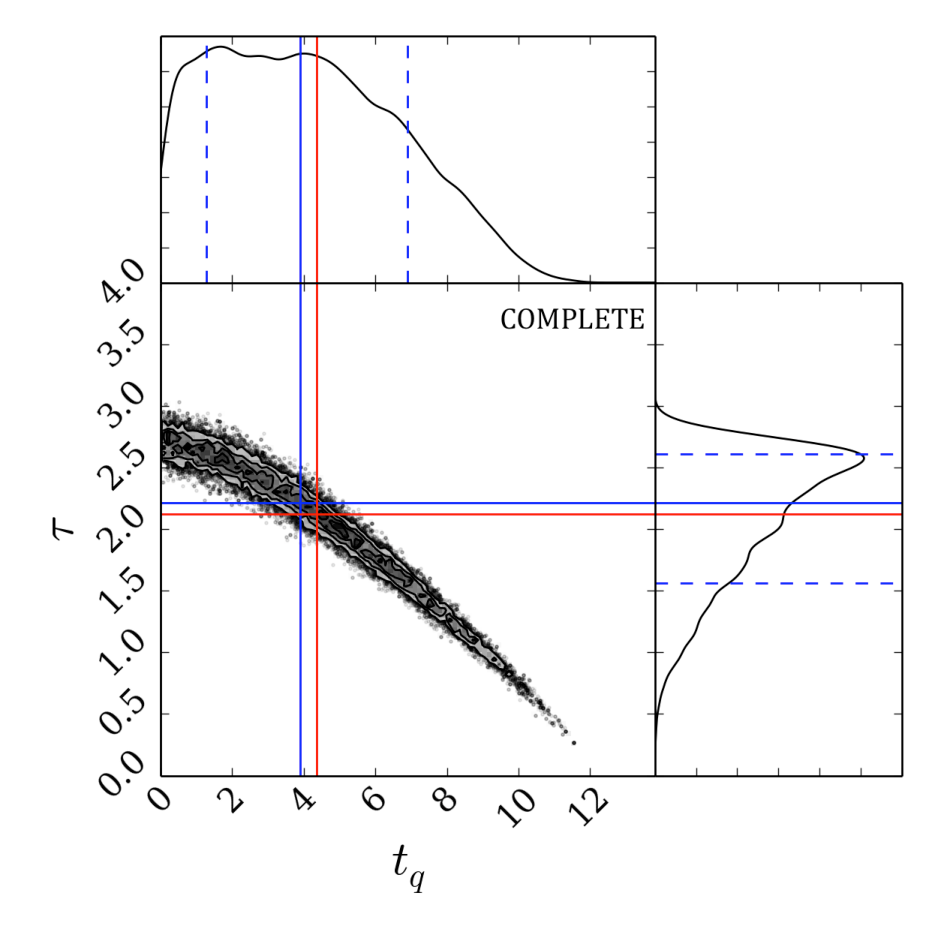
\includegraphics[width=0.49\textwidth]{starpy/corner_test_starfpy_full_sfh_function_0.pdf}
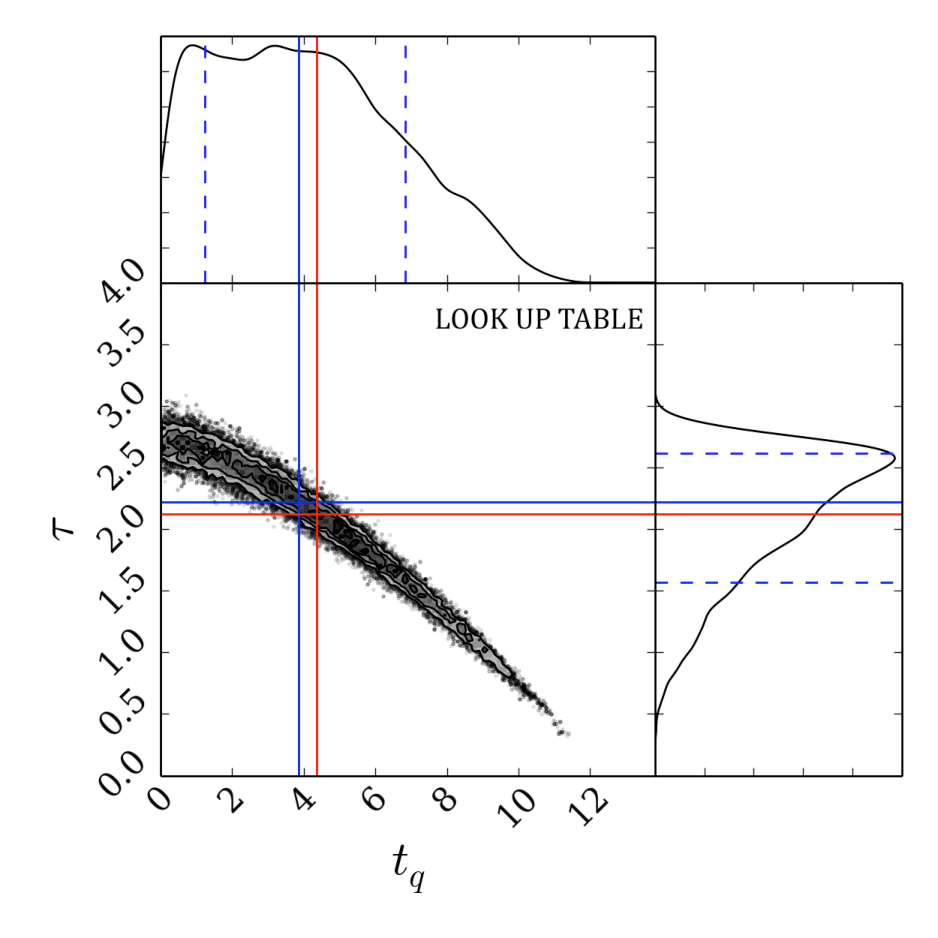
\includegraphics[width=0.49\textwidth]{starpy/corner_test_starfpy_lookup_0.pdf}}
\caption[Comparing complete and look-up table versions of \starpy]{Left panel: Results from \starpy ~for \underline{true} $t_q$ and $\tau$ values (red lines) using the complete function to calculate the predicted colour of a proposed set of $\theta$ values in each MCMC iteration. The median walker position (the 50th percentile of the Bayesian probability distribution) is shown by the solid blue line with the dashed lines encompassing $68\% (\pm 1\sigma)$ of the samples (the 16th and 84th percentile positions). The time taken to run for a single galaxy using this method is approximately 2 hours. Right panel: Results from \starpy ~for \underline{true} $t_q$ and $\tau$ values using a look up table generated from the complete function to calculate the predicted colour of a proposed set of $\theta$ values in each MCMC iteration. The time taken to run for a single galaxy using this method is approximately 2 minutes.}
\label{lookup}
\end{figure*}

\begin{table}
\centering{
\caption{Median walker positions (the 50th percentile; as shown by the blue solid lines in Figure~\ref{lookup}) found by \starpy ~ for a single galaxy, using the complete star formation history function and a look up table to speed up the run time. The errors quoted define the region in which $68\%$ of the samples are located, shown by the dashed blue lines in Figure~\ref{lookup}. The known true values are also quoted, as shown by the red lines in Figure~\ref{lookup}. All values are quoted to three significant figures.}
\begin{tabular*}{0.65\textwidth}{r @{\extracolsep{\fill}}ccc}
\multicolumn{1}{l}{} & \multicolumn{3}{c}{}                                          \\ \hline
                     & $t_q$                       & $\tau$                       &  \\ \hline
True                 & $4.37$                        & $2.12$                         &  \\
Complete             & $3.893 \pm^{3.014}_{2.622}$ & $2.215 \pm^{0.395}_{0.652}$ &  \\
Look up table        & $3.850 \pm^{2.988}_{2.619}$ & $2.218 \pm^{0.399}_{0.649}$ & \\ \hline
\end{tabular*}}
\label{median_lu}
\end{table}

I wish to consider the SFH model parameters for a large populations of galaxies across the colour magnitude diagram, however for each combination of $\theta$ values which \emph{emcee} proposes for a single galaxy, a new SFH must be built, prior to convolving it with the BC03 SPS models at the observed age and then predicted colours calculated from the resultant SED. For a single galaxy this takes up to 2 hours on a typical desktop machine for long Markov Chains. A 3-dimensional look-up table was therefore generated at $50 ~t^{obs}$, $100 ~t_{quench}$ and $100 ~\tau$ values; this was then interpolated over for a given observed galaxy's age and proposed $\theta$ values at each step in the Markov Chain. This ensured that a single galaxy takes approximately 2 minutes to run on a typical desktop machine. 

Figure~\ref{lookup} shows an example of how using the look up table in place of the full function does not affect the results to a significant level. Table~\ref{median_lu} quotes the median walker positions (the 50th percentile of the Bayesian probability distribution) along with their $\pm 1\sigma$ ranges for both methods in comparison to the true values specified to test \starpy. The uncertainties incorporated into the quoted values by using the look up table are therefore minimal with a maximum $\Delta = 0.043$.

Using this lookup table, each of the $126,316$ total galaxies in the \textsc{gz2-galex} sample was run through \starpy ~on multiple cores of a computer cluster to obtain the Markov Chain positions (analogous to $P(\theta_k|d_k)$) for each galaxy, $k$ (see Figure~\ref{one_example}). In each case the Markov Chain consisted of $100$ `walkers' which took $400$ steps in the `burn-in' phase and $400$ steps thereafter, at which point the MCMC acceptance fraction was checked to be within the range $0.25 < f_{acc} < 0.5$ (which was true in all cases). Due to the Bayesian nature of this method, a statistical test on the results is not possible; the output is probabilistic in nature across the entirety of the parameter space.

\section{POPSTARPY: studying populations of galaxies with STARPY}\label{popstarpy}

To study the SFH of a large population of galaxies, the individual galaxy walker positions output by \starpy ~(analogous to the posterior probability distribution) are combined across $[t, \tau]$ space. The Markov Chain walker positions are binned and weighted by their corresponding logarithmic posterior probability $\log [P(\theta_k|d_k)]$, provided by the \emph{emcee} package, in order to emphasise the features and differences between various populations. This weighting by $\log [P(\theta_k|d_k)]$ is to minimise the contribution of galaxies poorly fit by this exponentially declining SFH. This is no longer inference but merely a method to visualise the results across a population of galaxies.

I also discard those walker positions with a corresponding normalised posterior probability of $P(\theta_k|d_k) < 0.2$ in order to exclude galaxies which are not well fit by the quenching model, therefore galaxies in each sample which reside on the main sequence will not contribute to the final population distribution of quenching parameters. This raises the issue of whether I exclude a significant fraction of the \textsc{gz2-galex} sample and whether those galaxies reside in a specific location of the colour-magnitude. The fraction of galaxies which had all or more than half of their walker positions discarded due to low probability are shown in Table \ref{discardnum}. Using the $P(\theta_k|d_k) < 0.2$ constraint, $2.4\%$, $7.0\%$ and $5.4\%$ of green, red and blue galaxies respectively had \emph{all} of their walker positions discarded. 

This is not a significant fraction of either population, therefore the \starpy~ module is effective in fitting the majority of galaxies and this method of discarding walker positions ensures that poorly fit galaxies are removed from the analysis of the results. Figure \ref{discarded} shows that these galaxies with discarded walker positions are also scattered across the optical-NUV colour-colour diagram and therefore \starpy ~is also effective in fitting galaxies across this entire plane. 

\begin{table*}
\centering{
\caption{The number of galaxies in each population which had walker positions discarded due to low posterior probability values in order to exclude those galaxies from the analysis which were poorly fit by the SFH quenching model.}
\begin{tabular*}{0.95\textwidth}{p{4cm} @{\extracolsep{\fill}} ccc}
                                          & \textbf{Red Sequence}                                   & \textbf{Green Valley}                                  & \textbf{Blue Cloud}                                      \\ \hline
All walkers discarded                     & \begin{tabular}[c]{@{}c@{}}1420\\ (7.00\%)\end{tabular} & \begin{tabular}[c]{@{}c@{}}437\\ (2.41\%)\end{tabular} & \begin{tabular}[c]{@{}c@{}}3109\\ (5.37\%)\end{tabular}  \\
More than half walker positions discarded & \begin{tabular}[c]{@{}c@{}}2010\\ (9.92\%)\end{tabular} & \begin{tabular}[c]{@{}c@{}}779\\ (4.30\%)\end{tabular} & \begin{tabular}[c]{@{}c@{}}6669\\ (11.52\%)\end{tabular} \\ \hline
\end{tabular*}}
\label{discardnum}
\end{table*}

\begin{figure}
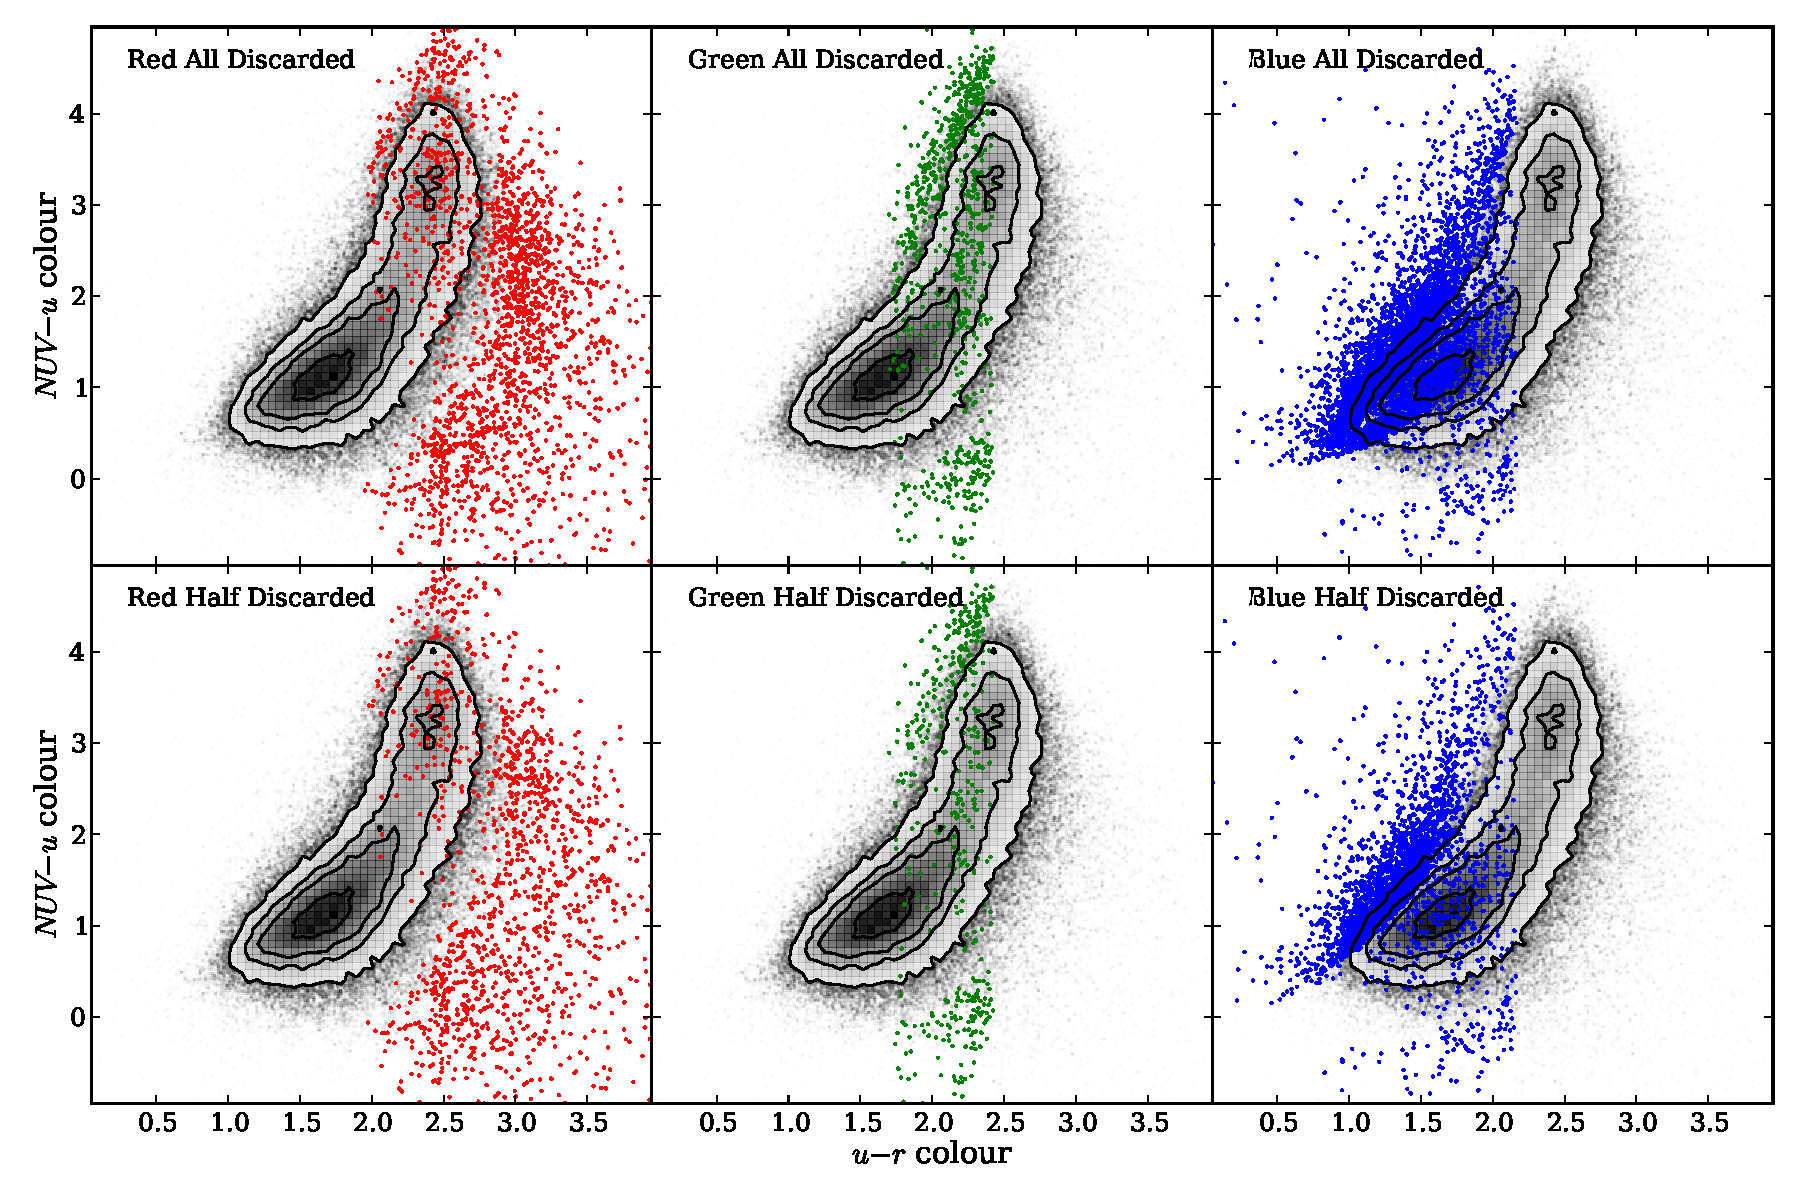
\includegraphics[width=0.9\textwidth]{starpy/discarded_galaxy_colour_colour.pdf}
\caption[Colours of discarded galaxies]{Contours show the full GZ2 subsample optical-NUV colour-colour diagram. The points show the positions of the galaxies which had all (top panels) or more than half (bottom panel) of their walker positions discarded due to their low probability for the red sequence (left), green valley (middle) and blue cloud (right).}
\label{discarded}
\end{figure}

Figure ~\ref{test_mosaic} shows how peaks in the histograms are found across all areas of the parameter space in both dimensions $[t, \tau]$, ensuring that any conclusions drawn from combined population distributions are due to a superposition of extended probability distributions, as opposed to a bimodal distribution of probability distributions across all galaxies.

The classifications from Galaxy Zoo 2 provide a uniquely powerful continuous measurements of a galaxy's morphology, therefore I utilise the debiased user vote fractions to obtain separate population density distributions for both smooth and disc galaxies. This is obtained by also weighting by the morphology vote fraction when the binned walker positions are combined. This ensures that the entirety of the population is used, with galaxies with a higher $p_d$ contributing more to the disc weighted than the smooth weighted population distribution. This negates the need for a threshold on the GZ2 vote fractions \citep[e.g., $p_d > 0.8$ as used in][]{schawinski14}. These distributions will be referred to as the population densities.

For example, the galaxy shown in Figure~\ref{one_example} would contribute almost evenly to both the smooth and disc parameters due to the GZ2 vote fractions. Since galaxies with similar vote fractions contain both a bulge and disc component, this method is effective in incorporating intermediate galaxies which are thought to be crucial to the morphological changes between early- and late-type galaxies. It was the consideration of these intermediate galaxies which was excluded from the investigation by \citet{schawinski14}.

\subsection{Alternative Hierarchical Bayesian approach}\label{althyper}

The approach presented above relies upon a visualisation of the SFHs across each population, with no inference involved beyond the use of \textsc{starpy} to derive the individual galaxy SFHs. An alternative approach to this problem would be to use a hierarchical Bayesian method to determine the `hyper-parameters' that describe the distribution of the parent population $\theta' = [t_q', \tau']$ that each individual galaxy's SFH is drawn from. 

The posterior PDF for $\vec{\theta}'$ to describe such a galaxy population:
\begin{equation}\label{hyper}
P(\vec{\theta}'|\vec{d}) = \frac{P(\vec{d}|\vec{\theta}')P(\vec{\theta}')}{P(\vec{d})}, 
\end{equation}
where $\vec{d}$ represents all of the optical and NUV colour data in a population $\{\vec{d}_k\}$. For one galaxy, $k$, the marginalised likelihood is:
\begin{equation}\label{one}
P(d_k|\vec{\theta}') = \iint \! P(d_k|t_k, \tau_k) P(t_k, \tau_k|\vec{\theta}') \ \mathrm{d}t_k ~ \mathrm{d}\tau_k
\end{equation}
and for all galaxies, $N$, therefore: 
\begin{equation}
P(\vec{d}|\vec{\theta}') = \prod_k^N P(d_k|\vec{\theta}').
\end{equation}

Using \textsc{starpy}~ for an individual galaxy, $k$ the output is the `interim' posterior $P(t_k, \tau_k|d_k)$ which I can relate to $P(d_k|t_k, \tau_k)$  so that:

\begin{equation}\label{marg}
P(d_k|\vec{\theta}') = \iint  \! P(t_k, \tau_k|d_k) . P(d_k) . \frac{P(t_k, \tau_k|\vec{\theta}')}{P(t_k, \tau_k)} \ \mathrm{d}t_k ~ \mathrm{d}\tau_k.
\end{equation}
In order to calculate this I draw $N_s$ random samples, $r$, from each interim posterior, $P(t_k, \tau_k|d_k)$ so that Equation \ref{marg} can be expressed as a sum over a number of random samples, $N_s$ (as with the calculation of an expected mean):
\begin{equation}\label{imp}
P(d_k|\vec{\theta}') = \frac{P(d_k)}{N_s} \sum_r^{N_s} \frac{P(t_{k,r}, \tau_{k,r}|\vec{\theta}')}{P(t_k, \tau_k)},
\end{equation}
for the $r^{th}$ sample of $N_s$ total samples taken from one galaxy's, $k$,  interim posterior PDF. This fraction is known as the `importance weight', $w_r$, in importance sampling. 

However, I also have two morphological vote fractions that I can weight by to determine separate hyper-parameters, $\vec{\theta}' = [\vec{\theta}'_d, \vec{\theta}'_s]$, for both disc, $d$, and smooth, $s$, galaxies. Therefore:

\begin{equation}\label{morphimp}
w_r = \frac{P(t_{k,r}, \tau_{k,r}|\vec{\theta}')}{P(t_k, \tau_k)} =  \frac{p_{d,k} P(t_{k,r}, \tau_{k,r}|\vec{\theta}'_d) + p_{s,k} P(t_{k,r}, \tau_{k,r}|\vec{\theta}'_s)}{P(t_k, \tau_k)}
\end{equation} 

If we substitute equation \ref{imp} into equation \ref{hyper} we find that the $P(d_k)$ terms cancel and we are left with:
\begin{equation}
P(\vec{\theta}'|\vec{d}) = P(\vec{\theta}')~\prod_k^N \frac{1}{N_{s,k}} \sum_r^{N_s} w_r ,
\end{equation}
where $P(\vec{\theta}')$ is the assumed prior on the hyper-parameters, which is assumed to be uniform.

\begin{figure}
\begin{centering}
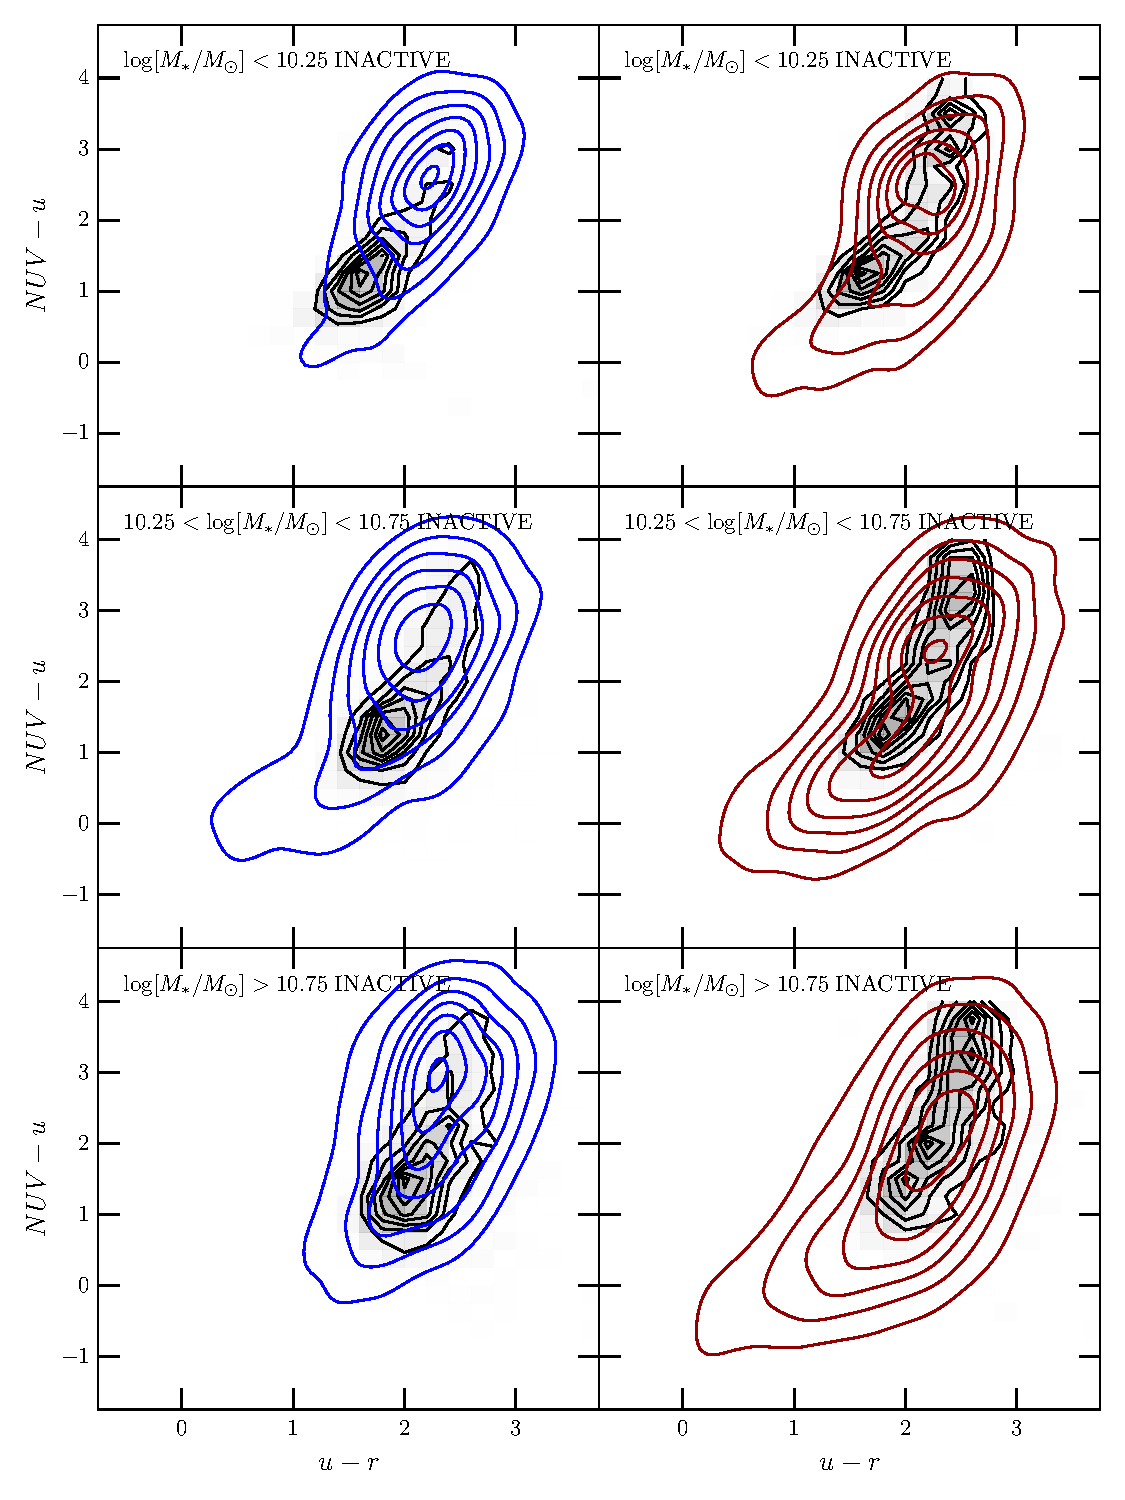
\includegraphics[width=0.8\textwidth]{starpy/figc2b.pdf}
\caption[Replica colour-colour distributions using a hierarchical method]{Optical-NUV colour-colour diagrams for the \textsc{inactive} galaxies shown by the black contours, split into low mass (top), medium mass (middle) and high mass (bottom) galaxies weighted by $p_d$ (left) and $p_s$ (right). Kernel smoothing has been applied to the overlaid replica datasets, which are created by sampling from the \textbf{inferred 2 component Gaussian mixture model hierarchical parent distributions}. Gaussian random noise is also added to the inferred colours, with a mean and standard deviation of the errors on the observed colours of the respective sample. Contours are shown for samples taken from the disc (blue) and smooth weighted (red) inferred hierarchical distributions.}
\label{replica}
\end{centering}
\end{figure}

\begin{figure}
\begin{centering}
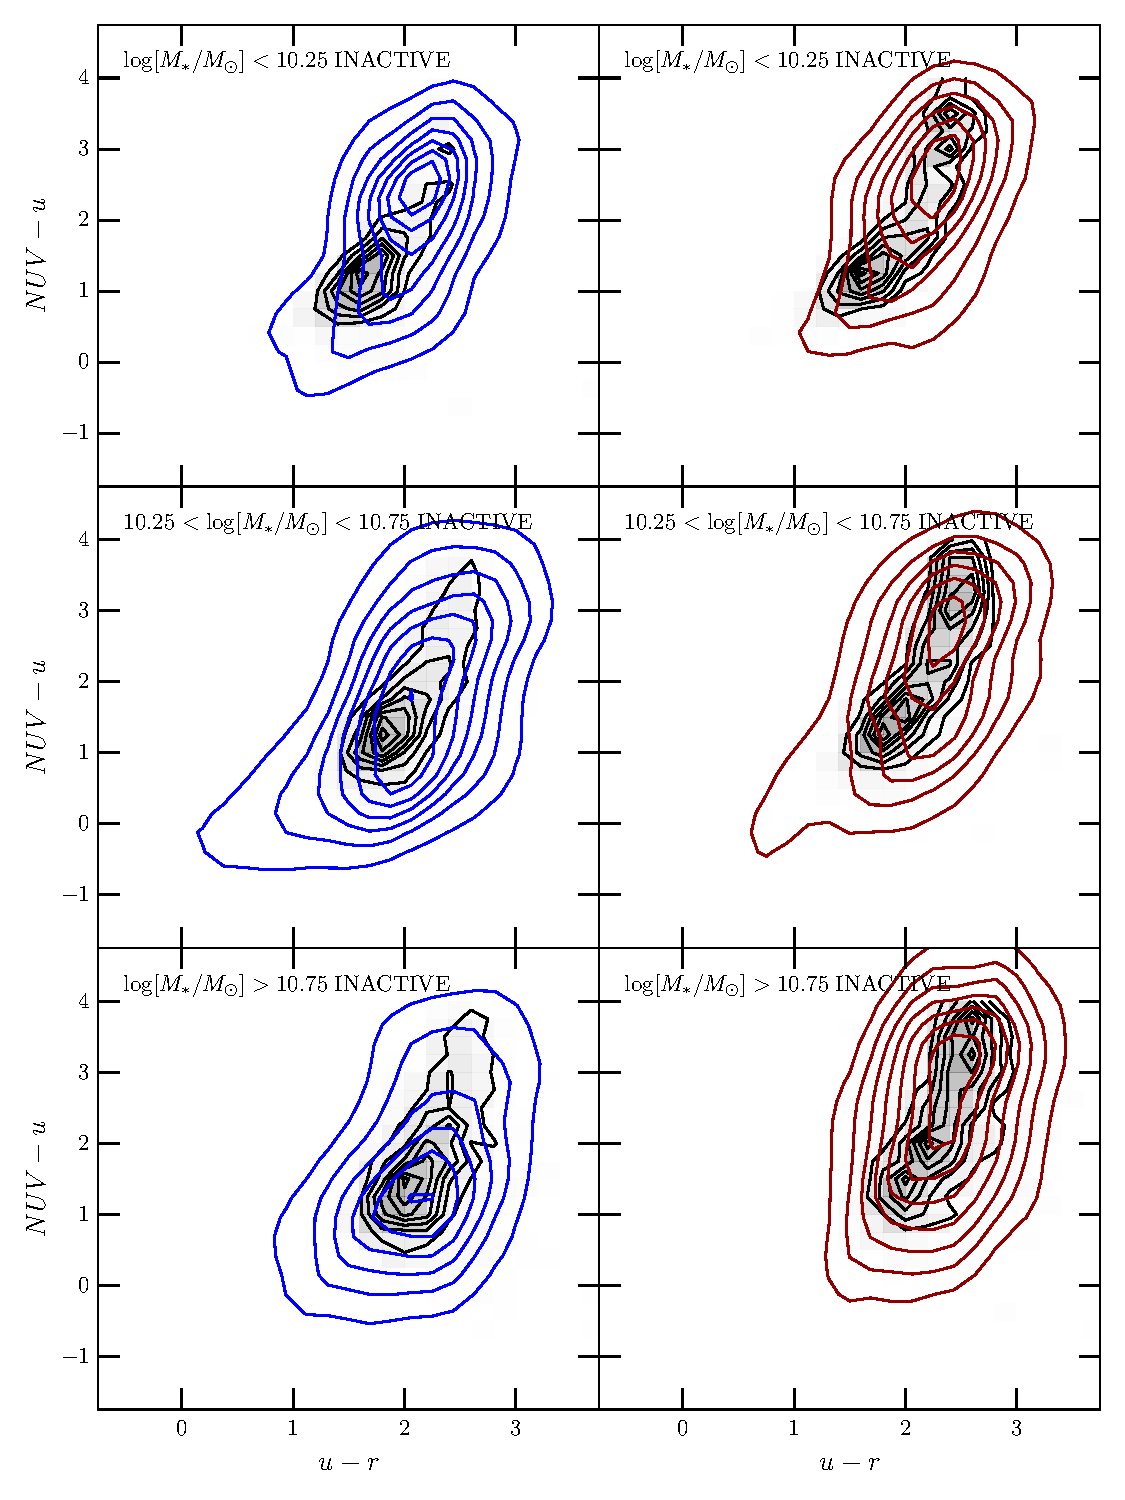
\includegraphics[width=0.8\textwidth]{starpy/figc3b.pdf}
\caption[Replica colour-colour distributions using the \textsc{popstarpy} method]{Optical-NUV colour-colour diagrams for the \textsc{inactive} galaxies shown by the black contours, split into low mass (top), medium mass (middle) and high mass (bottom) galaxies weighted by $p_d$ (left) and $p_s$ (right). Kernel smoothing has been applied to the overlaid replica datasets, which are created by sampling from the \textbf{\textsc{popstarpy} population density distributions described in Section~\ref{popstarpy}}. Gaussian random noise is also added to the inferred colours, with a mean and standard deviation of the errors on the observed colours of the respective sample. Contours are shown for samples taken from the disc (blue) and smooth weighted (red) inferred hierarchical distributions.}
\label{replicapop}
\end{centering}
\end{figure}

This approach is heavily dependent on what shape is assumed for the hyper-distribution; a decision which is not trivial. It is often common for this function to take the form of a multi-component Gaussian mixture model \citep{mackay03, lahav00}. For example a two component Gaussian mixture model in $[t, \tau]$ space is described by eight hyper-parameters for a single morphology, $\vec{\theta}' = [\mu_{t,1}, \sigma_{t,1}, \mu_{\tau,1}, \sigma_{\tau,1}, \mu_{t,2}, \sigma_{t,2}, \mu_{\tau,2}, \sigma_{\tau,2}]$. This approach assumes no covariance between hyper-parameters for simplicity. The equations outlined above, combined with MCMC methods can be used to infer these $8 \vec{\theta}'$ parameters from which the hierarchical population distribution can be determined. 

%I used this assumption of a two component Gaussian mixture model, to infer the population parameters for both the \textsc{agn-host} and \textsc{inactive} populations and the results are shown in Figure~\ref{method3}. These results were produced by drawing $N_s = 100$ random samples from each galaxy, $k$, in each mass bin. I plot the distributions for a given morphology by taking the median value of the posterior distribution for each of the 8 parameters describing the two component Gaussian mixture. I can see in Figure~\ref{method3} that this hierarchical method produces similar distributions for the \textsc{agn-host} and \textsc{inactive} samples. This finding is not expected given the differences between the two samples in colour-colour space seen in Figure~\ref{colcol}. 

%\begin{figure}
%\includegraphics[width=0.48\textwidth]{figc1a.pdf}
%\includegraphics[width=0.48\textwidth]{figc1b.pdf}
%\caption[8pt]{Hierarchical-posterior PDF of the quenching time ($t_q'$, top) and rate ($\tau'$, bottom) population parameters, normalised so that the areas under the curves are equal. \textsc{agn-host} (left) and \textsc{inactive} (right) galaxies are split into low (top), medium (middle) and high (bottom) mass, weighted for smooth (red dashed) and disc (blue solid) galaxies. A low (high) value of $t_q'$ corresponds to the early (recent) Universe. A small (large) value of $\tau'$ corresponds to a rapid (slow) quench.}
%\label{method3}
%\end{figure}

In order to test whether this assumption of a multi-component Gaussian mixture model is appropriate, I sampled the inferred hierarchical distributions to produce replica datasets in optical-NUV colour space. These are shown here in Figure~\ref{replica}  in comparison to the observed colour-colour distributions of the \textsc{inactive} sample (a subset of $\sim6,000$ galaxies from the \textsc{gz2-galex} sample, see Section~\ref{agnfeedback}). For all masses and morphologies the replicated $u-r$ and $NUV-u$ colours do not accurately match the observed data. 


I also varied the value of $N_s$ and found that increasing the number of samples drawn did not improve this fit for the \textsc{inactive} population. Similarly increasing the number of components in the Gaussian mixture model did not immediately improve the accuracy of the fit.  I therefore concluded that this functional form of the population distribution was unsatisfactory. %An extensive exploration of a wide variety of functional forms is necessary to ensure the correct conclusions are drawn from the data. Such an investigation is beyond the scope of this paper. 

The \textsc{popstarpy} approach described in section \ref{popstarpy} was motivated by the investigation increasing the number of samples, $N_s$ drawn from the posterior of each galaxy, k, until the point where all the samples were drawn. Instead of attempting to infer parameters to describe this distribution, as above, I presented the distribution itself (as described in Section \ref{popstarpy}).  The distributions produced by this visualisation method reveal the complexity that the parent distribution must describe which, as concluded earlier, cannot be effectively modelled.

I also tested whether the \textsc{popstarpy} method is reasonable by producing replica datasets in optical-NUV colour space, as before, by drawing $1000$ $[t, \tau]$ values from the population density distributions derived for the \textsc{inactive} sample (see Section~\ref{agnfeedback}). These replica datasets are shown here in Figure~\ref{replicapop} in comparison to the observed colour-colour distributions of the \textsc{inactive} sample. Comparing these replica colours in Figure~\ref{replicapop}, with those produced by drawing from the inferred hierarchical distributions, shown in Figure~\ref{replica}, they can be seen to produce a more accurate match to the observed data for the majority of masses and morphologies. 

Considering these issues with assuming a functional form for the hierarchical parent distribution, an expansion on this approach would be to perform `heat map optimization', similar to image reconstruction, to determine the parent distribution for a given population. Each pixel would need a prior (e.g. a basic entropic prior) and the heat map would sum to unity. This is a significant expansion upon the work presented here and is something the author wishes to investigate in future work.

For the results presented in the following chapters, I therefore use the \textsc{popstarpy} method to visualise the population distribution, rather than quoting inferred values to describe it.



\chapter{The morphological dependance of quenching}\label{morph}

\emph{The work in the following chapter has been published in \citet{smethurst15}.}


By studying the galaxies which have just left the `main sequence' of star formation (see top panel of Figure \ref{sfr_mass_col}), the nature of the quenching mechanisms which cause this departure can be probed. By investigating the \emph{amount} of quenching that has occurred in the blue cloud, green valley and red sequence; and by comparing that amount across the three populations, constraints can be applied to the many possible quenching mechanisms outlined in Chapter \ref{intro}. 

I have been motivated by a recent result suggesting there are two contrasting evolutionary pathways through the green valley for different morphological types (\citealt{schawinski14}, hereafter S14). S14 used the same exponentially declining star formation model, as described in Section~\ref{qmod}, to obtain predicted optical and NUV colours for four possible SFHs through the green valley; two with fast quenching rates ($\tau = [0.001, 0.25]$ $\rm{Gyr}$) and two with slower quenching rates ($\tau = [1, 2.5]$ $\rm{Gyr}$). These predicted colours were then compared to observed colours of early- and late-type green valley galaxy colours on an optical-NUV colour-colour diagram. They concluded from this diagram that late-type galaxies quench with a slower rate and form a nearly static disc population in the green valley, whereas early-type galaxies quench with very rapid rates, transitioning through the green valley and onto the red sequence in $\sim 1$~Gyr \citep{Wong12}. 

Although this result of morphologically dependent quenching is intriguing, the work of S14 is hindered for the following reasons: (i) the incompleteness of the galaxy sample; only definitively early- ($p_s \geq 0.8$) and late-type ($p_s \leq 0.8$) galaxies were studied, whereas galaxies of intermediate morphology were excluded, and (ii) the lack of statistics to support the conclusions. Here I use the same toy model but implement \starpy ~in order to statistically study the star formation histories of galaxies of all morphologies across the colour magnitude diagram.


\section{Defining the Green Valley}\label{defGV}

To define which of the $126, 316$ galaxies of the \textsc{gz2-galex} sample are in the green valley, I looked to previous definitions in the literature defining the separation between the red sequence and blue cloud. For example, \citet{Baldry04} traced this bimodality with a large sample of $66,846$ local SDSS galaxies ($0.004 < z < 0.08$) by fitting double-peaked Gaussians to the colour magnitude diagram. Their relation between the $u-r$ colour, $C'_{ur}$, and r-band magnitude, $M_r$, to define the colour cut between the blue and red galaxy populations is defined in their Equation 11 as:
\begin{equation}\label{eqgv}
C'_{ur}(M_{r}) = 2.06 - 0.244 \tanh \left( \frac{M_r + 20.07}{1.09}\right).
\end{equation}

Due to the necessity for NUV photometry in this study, matching to GALEX removed typical `red and dead' galaxies from the \textsc{gz2-galex} sample. This is apparent in the optical $u-r$ colour histograms shown in the right panels of Figure \ref{fig:cmgvsplit}; the \textsc{gz2-galex} sample is split in bins of absolute r-band magnitude and for each bin the position of the green valley at that $M_r$, as defined by \citet{Baldry04} is shown. For the \textsc{gz2-galex} sample at brighter r-band magnitudes (i.e. larger mass), this definition of the green valley seems to intersect with the observed peak at red colours. 

\begin{figure}
\centering{
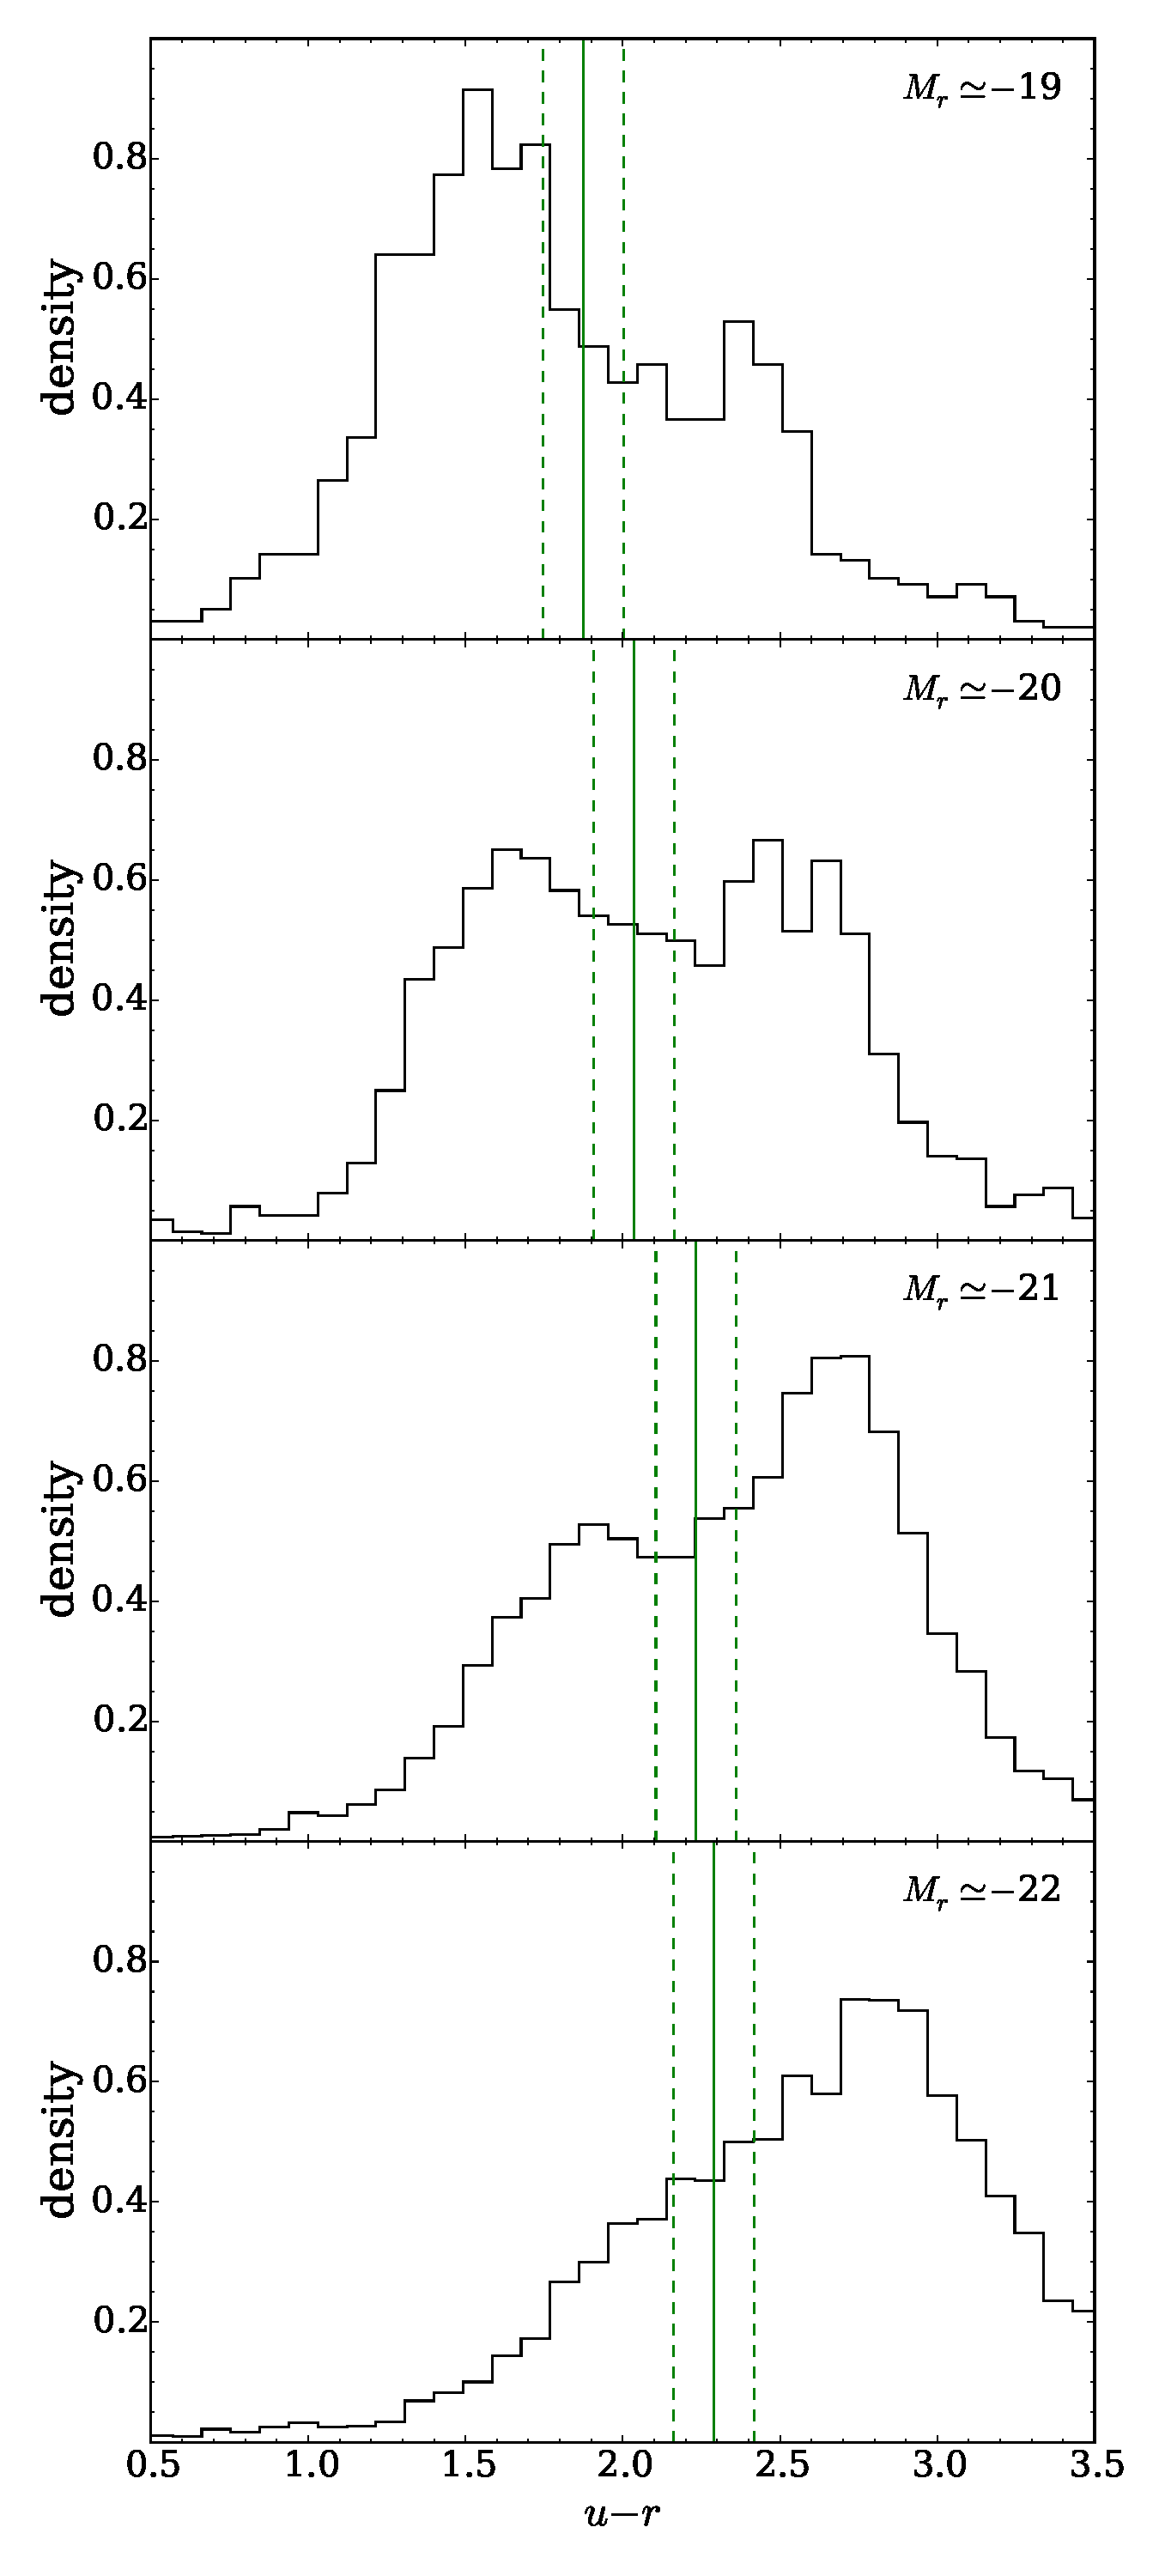
\includegraphics[width=0.49\textwidth]{morphology/sdss_hist_slice.pdf}
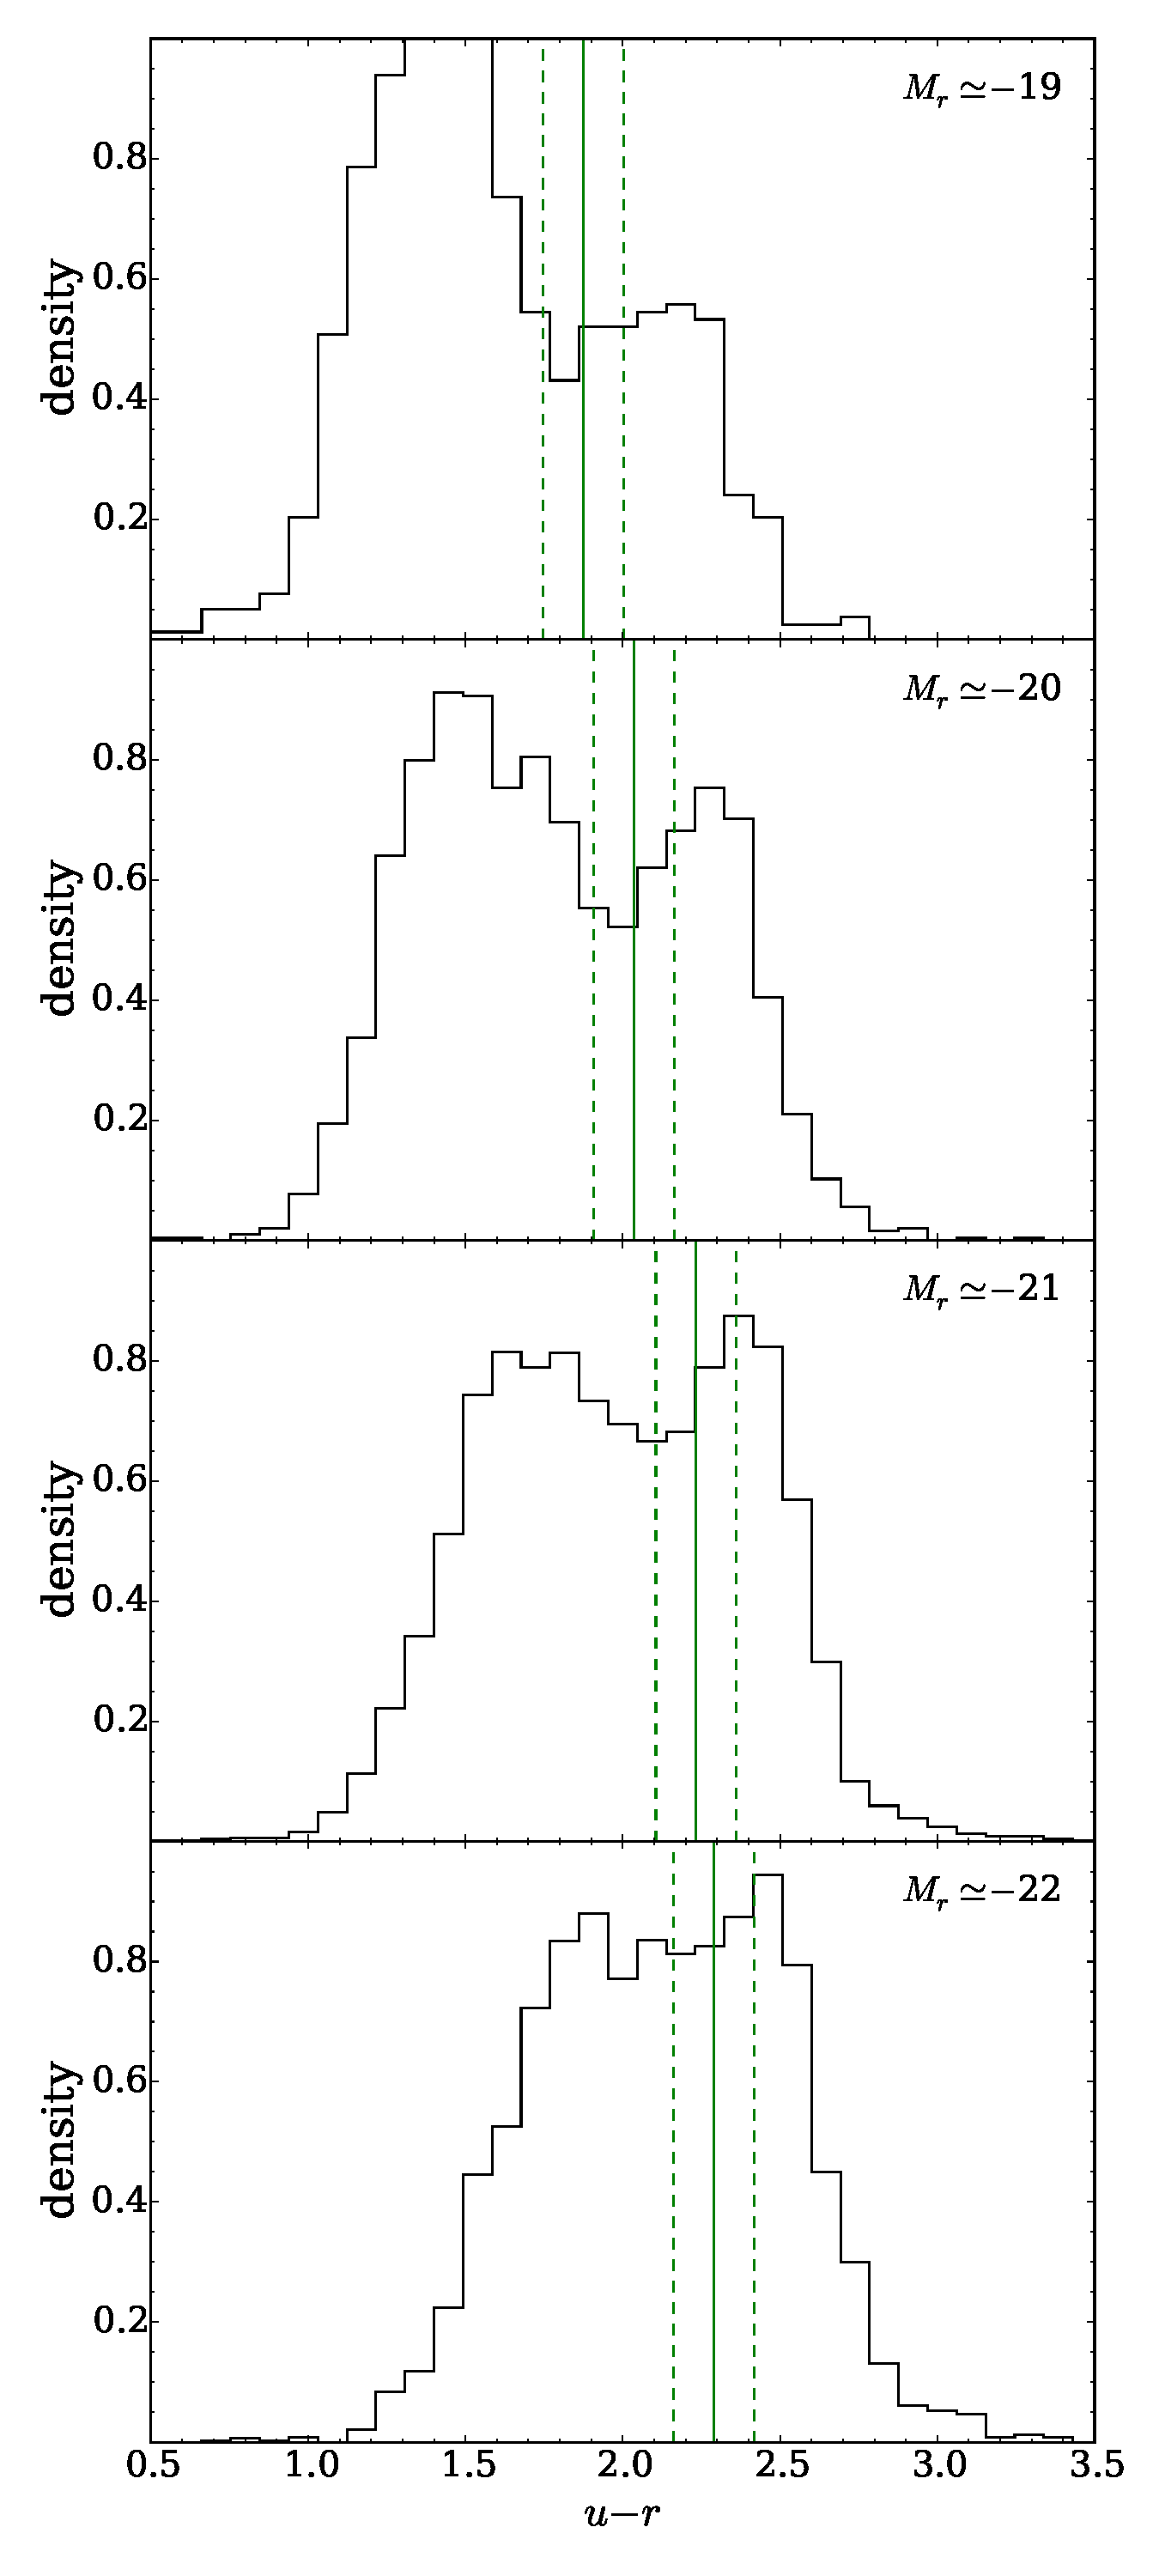
\includegraphics[width=0.49\textwidth]{morphology/galzoo_hist_slice.pdf}}
\caption[Optical $u-r$ colour histograms in absolute r-band magnitude slices of the \textsc{gz2-galex} and Baldry et al. (2004) complete SDSS samples]{Optical $u-r$ colour histograms, sliced in absolute r-band magnitude for a complete SDSS sample (MPA-JHU catalog; left) and for the \textsc{gz2-galex} sample (right). In each panel the definition between the blue cloud and the red sequence from \citet{Baldry04} is shown by the dashed line (as defined in Equation~\ref{eqgv}); the solid lines show $\pm 1\sigma$ either side of this definition.}
\label{fig:cmgvsplit}
\end{figure}

However, for the larger SDSS sample (from the MPA-JHU catalog; \citealt[][left panels of Figure~\ref{fig:cmgvsplit}]{kauffmann03, brinchmann04}) the \citet{Baldry04} green valley definition does not intersect with the peak at red colours, as this sample is complete, containing the high mass typical `red and dead' galaxies of the red sequence. It would therefore not be appropriate to define the green valley by a visual fit to the colour magnitude diagram for this study (this method was used in S14 and adopting it here would have allowed for a direct comparison to this previous work) as this would cause green valley galaxies to be misclassified as red sequence.

I therefore adopt the \citet{Baldry04} green valley definition for this study, which is shown in Figure~\ref{fig:CMGV} by the dashed line in comparison to both the \textsc{gz2-galex} sample (left) and the SDSS data used for the fit by \cite[][right]{Baldry04}. Any galaxy within $\pm 1\sigma$ of this relationship, shown by the solid lines in Figure~\ref{fig:CMGV}, is therefore considered a green valley galaxy. 

\begin{figure*}
\centering{
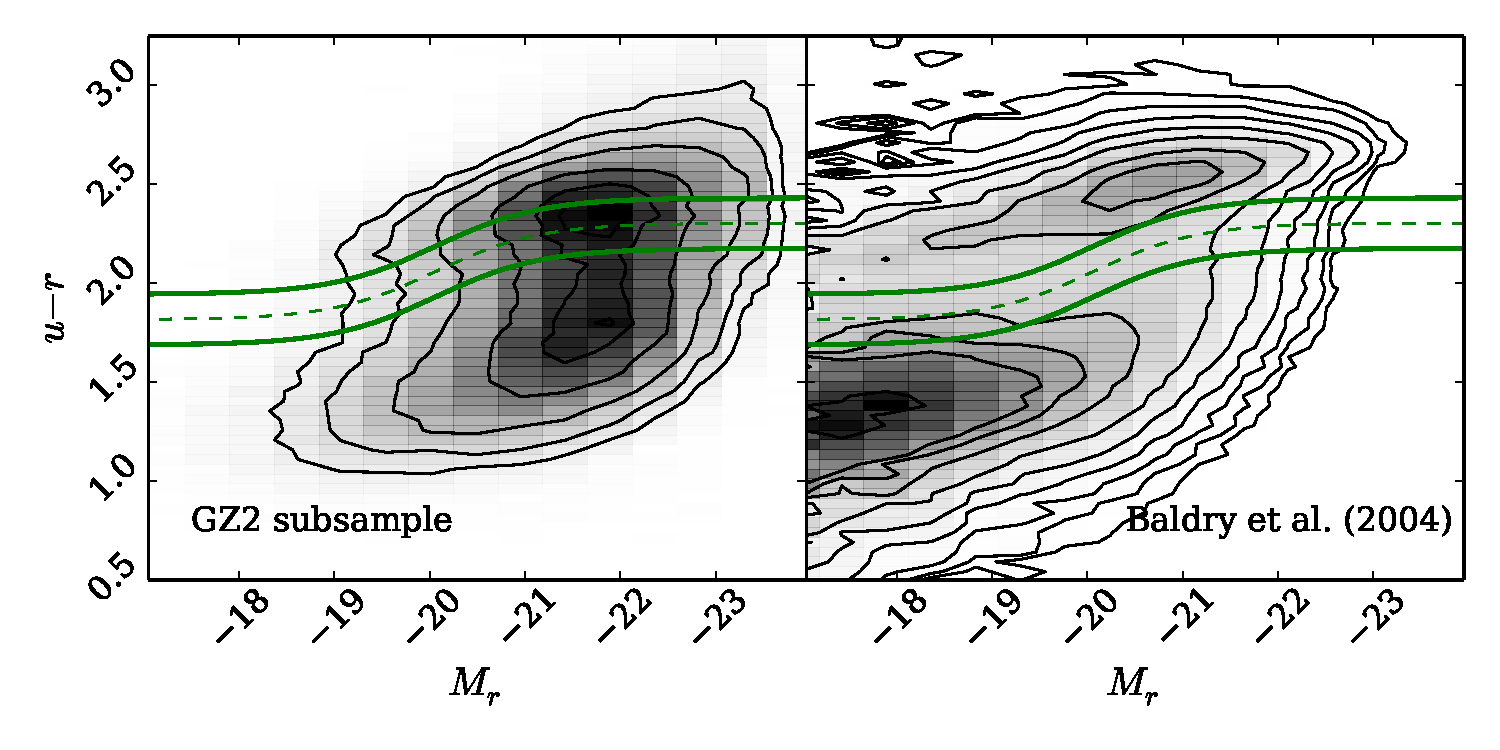
\includegraphics[width=\textwidth]{morphology/col_mag_GV_Baldry_data.pdf}}
\caption[Colour-magnitude diagram showing the location of the Baldry et al. (2004) green valley definition]{Colour-magnitude diagram for the \textsc{gz2-galex} sample (left) and the SDSS sample from \citet[][right]{Baldry04}. In both panels the definition between the blue cloud and the red sequence from \citet{Baldry04} is shown by the dashed line, as defined in Equation~\ref{eqgv}. The solid lines show $\pm 1\sigma$ either side of this definition; any galaxy within the boundary of these two solid lines is considered a green valley galaxy. The lack of red sequence galaxies due to the necessity for NUV GALEX colours skews the apparent location of the green valley in the \textsc{gz2-galex} sample, therefore a literature definition of the green valley is used to ensure galaxies are correctly classified.}
\label{fig:CMGV}
\end{figure*}

However, although the galaxies identified as residing on the red sequence within the \textsc{gz2-galex} sample have NUV detections, this does not mean they are not representative of a typical red sequence `red and dead' galaxy. \cite{ko13} show that in a sample of quiescent red-sequence galaxies without $\mathrm{H}\alpha$ emission (i.e. without spectral indication of recent star formation), $26\%$ show NUV excess emission and that the fraction with recent star formation is $39\%$. Of the $48\%$ of \textsc{gz2-galex} galaxies classified as below the main sequence using the definition from \citet[][see Section~\ref{qmod}]{peng10}, $44\%$ of these galaxies lie on the red sequence ($94\%$ of all the red sequence galaxies in the \textsc{gz2-galex} sample; see Table ~\ref{table:qsubs}). I am therefore confident that the \textsc{gz2-galex} sample will include galaxies from across the entirety of the colour magnitude diagram. 

The decomposition of the \textsc{gz2-galex} sample into red sequence, green valley and blue cloud galaxies is shown in Tables~\ref{table:subs} and \ref{table:qsubs} along with further division by galaxy type and SFR (where available for the \textsc{gz2-galex} sample from the MPA-JHU catalog) respectively. The tables also list the definitions I adopt henceforth for early-type ($p_s~ \geq~0.8$), late-type ($p_d~ \geq~0.8$), smooth-like ($p_s~ >~0.5$), disc-like ($p_d~ >~0.5$), quenched ($\rm{SFR}$ $ < P - 5\sigma$), quenching ($P - 5\sigma < \rm{SFR}$ $< P - \sigma$) and star forming  ($\rm{SFR}$ $> P -\sigma$) galaxies, where $P$ is the SFR as defined by \citet{peng10} for a given stellar mass and observed time (see Equation \ref{eq:peng}). 

\begin{table}
\caption{Table showing the decomposition of the \textsc{gz2-galex} sample by galaxy type into the subsets of the colour-magnitude diagram.}
\begin{tabular*}{\textwidth}{l @{\extracolsep{\fill}}cccc}
\hline
\begin{tabular}[c]{@{}c@{}} {\color{white} -} \\ {\color{white} -}  \end{tabular} & All                                                      & Red Sequence                                              & Green Valley                                              & Blue Cloud \\  \hline 
Smooth-like ($p_s > 0.5$)        & \begin{tabular}[c]{@{}c@{}}42453\\ (33.6\%)\end{tabular} & \begin{tabular}[c]{@{}c@{}}17424\\ (61.9\%)\end{tabular}  & \begin{tabular}[c]{@{}c@{}}10687\\ (44.6\%)\end{tabular}   & \begin{tabular}[c]{@{}c@{}}14342\\ (19.3\%)\end{tabular}  \\ 
Disc-like ($p_d > 0.5$)          & \begin{tabular}[c]{@{}c@{}}83863\\ (80.7\%)\end{tabular} & \begin{tabular}[c]{@{}c@{}}10722\\ (38.1\%)\end{tabular}   & \begin{tabular}[c]{@{}c@{}}13257\\ (55.4\%)\end{tabular}  & \begin{tabular}[c]{@{}c@{}}59884\\ (47.4\%)\end{tabular}  \\
Early-type ($p_s \geq 0.8$) & \begin{tabular}[c]{@{}c@{}}10517\\ (8.3\%)\end{tabular}  & \begin{tabular}[c]{@{}c@{}}5337\\ (18.9\%)\end{tabular}    & \begin{tabular}[c]{@{}c@{}}2496\\ (10.4\%)\end{tabular}    & \begin{tabular}[c]{@{}c@{}}2684\\ (3.6\%)\end{tabular}    \\
Late-type ($p_s \geq 0.8$)  & \begin{tabular}[c]{@{}c@{}}51470\\ (40.9\%)\end{tabular} & \begin{tabular}[c]{@{}c@{}}4493\\ (15.9\%)\end{tabular}    & \begin{tabular}[c]{@{}c@{}}6817\\ (28.5\%)\end{tabular}    & \begin{tabular}[c]{@{}c@{}}40430\\ (54.4\%)\end{tabular}  \\ \hline
\textbf{Total}                       & \begin{tabular}[c]{@{}c@{}}\textbf{126316} \\ (100.0\%)\end{tabular}                                                & \begin{tabular}[c]{@{}c@{}}28146 \\ (22.3\%)\end{tabular} & \begin{tabular}[c]{@{}c@{}}23944 \\ (18.9\%)\end{tabular} & \begin{tabular}[c]{@{}c@{}}74226 \\ (58.7\%)\end{tabular} \\\hline
\end{tabular*}
\label{table:subs}
\end{table}


\begin{table}
\caption{Table showing the decomposition of the \textsc{gz2-galex} sample by their star formation rate in the subsets of the colour-magnitude diagram.}
\begin{tabular*}{\textwidth}{l @{\extracolsep{\fill}}cccc}
\hline
\begin{tabular}[c]{@{}c@{}} {\color{white} -} \\ {\color{white} -}  \end{tabular} 		& All                                                      						& Red Sequence                                              			& Green Valley                                             			 & Blue Cloud \\  \hline 
\begin{tabular}[l]{@{}l@{}}Quenched\\ ($\rm{SFR} < P - 5\sigma$) \end{tabular}	& \begin{tabular}[c]{@{}c@{}}24278\\ (19.7\%)\end{tabular} 			& \begin{tabular}[c]{@{}c@{}}17018\\ (60.9\%)\end{tabular}    & \begin{tabular}[c]{@{}c@{}}6440\\ (27.5\%)\end{tabular}    & \begin{tabular}[c]{@{}c@{}}820\\ (1.1\%)\end{tabular}  \\ 
\begin{tabular}[l]{@{}l@{}}Quenching\\ ($P - 5\sigma < \rm{SFR} < P - \sigma$) \end{tabular}	 & \begin{tabular}[c]{@{}c@{}}34743\\ (28.2\%)\end{tabular}			 & \begin{tabular}[c]{@{}c@{}}9277\\ (33.1\%)\end{tabular}    & \begin{tabular}[c]{@{}c@{}}12181\\ (51.9\%)\end{tabular}    & \begin{tabular}[c]{@{}c@{}}13285\\ (18.6\%)\end{tabular}  \\ 
\begin{tabular}[l]{@{}l@{}}Star Forming  \\ ($\rm{SFR} > P -\sigma$) \end{tabular} & \begin{tabular}[c]{@{}c@{}}63957\\ (52.0\%)\end{tabular} 			& \begin{tabular}[c]{@{}c@{}}1665 \\ (5.9\%)\end{tabular}    & \begin{tabular}[c]{@{}c@{}}4828\\ (20.6\%)\end{tabular}    & \begin{tabular}[c]{@{}c@{}}57464\\ (80.3\%)\end{tabular}  \\ \hline
\textbf{Total}                       		& \begin{tabular}[c]{@{}c@{}}\textbf{122,978} \\ (100.0\%)\end{tabular} & \begin{tabular}[c]{@{}c@{}}27960 \\ (22.7\%)\end{tabular} & \begin{tabular}[c]{@{}c@{}}23449 \\ (19.1\%)\end{tabular} & \begin{tabular}[c]{@{}c@{}}71569 \\ (58.2\%)\end{tabular} \\\hline
\end{tabular*}
\label{table:qsubs}
\end{table}

Figure~\ref{sfr_mass_sub} shows the SFR against the stellar mass for the \textsc{gz2-galex} sample (where available from the MPA-JHU catalog) by splitting it into blue cloud, green valley, red sequence, late- and early-type populations. This figure confirms that the green valley galaxies in the \textsc{gz2-galex} sample are indeed a population which have either left, or begun to leave, the star forming `main sequence' or have some residual star formation still occurring.

\begin{figure*}
\centering{
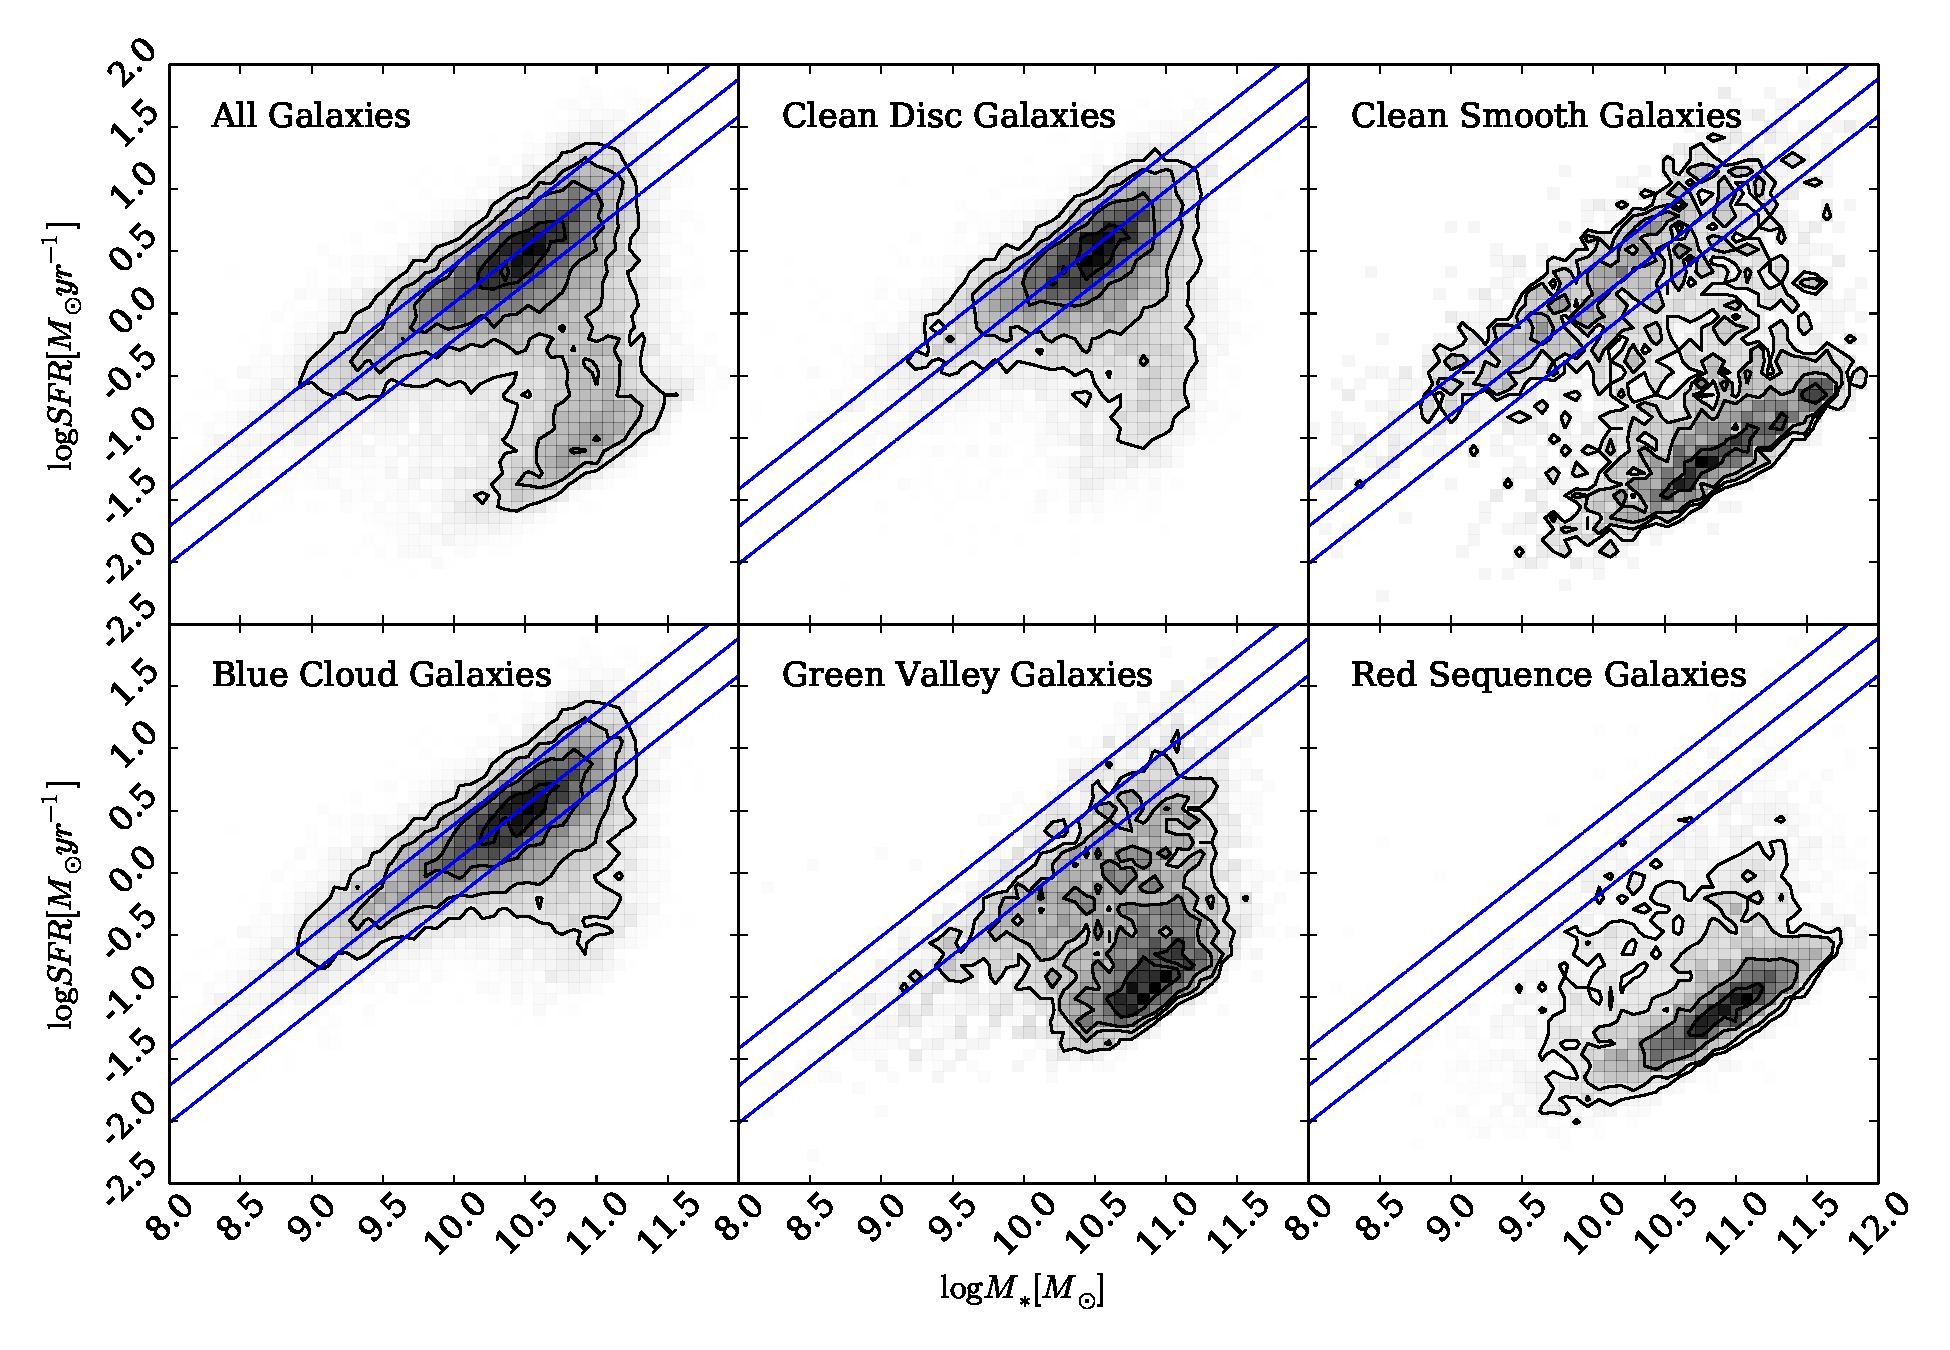
\includegraphics[width=\textwidth]{morphology/sfr_mass_subsets.pdf}}
\caption[SFR-stellar mass plane split by morphology and colour]{Star formation rate against stellar mass for the different populations of galaxies (top row, left to right: all galaxies, late-type galaxies, early-type galaxies; bottom row, left to right: blue cloud, green valley and red sequence galaxies) and how they contribute to the star forming sequence (from \citet{peng10}, shown by the solid blue line with 0.3 dex scatter by the dashed lines). Based on positions in these diagrams, the green valley does appear to be a transitional population between the blue cloud and the red sequence. Detailed analysis of star formation histories can elucidate the nature of the different populations' pathways through the green valley.}
\label{sfr_mass_sub}
\end{figure*}


\section{Results}\label{sec:morphresults}

The population density distributions for both smooth and disc weighted populations in the red sample, green valley and blue cloud are shown in Figures~\ref{red_s},~\ref{green_v} \&~\ref{blue_c} respectively. The full two dimensional distributions are shown in each case, along with a histogram showing the one dimensional projection for each parameter, $[t, \tau]$. The percentages shown in Figures~\ref{red_s},~\ref{green_v} \&~\ref{blue_c} are calculated as the fractions of the population densities located in each region of parameter space for a given population. 

Since the sample contains such a large number of galaxies, a peak in the population densities will be caused by a large number of galaxies with peaks in their individual posterior distribution at that location in parameter space. This will overwhelm contributions to this area of the population density from galaxies where this region of parameter space is not dominant in their individual posterior distributions. Therefore these fractions can be interpreted as broadly equivalent to the percentage of galaxies in a given population undergoing quenching within the stated timescale range. Although this is not quantitatively exact, it is nevertheless a useful framework for interpreting the population densities.

Figure~\ref{fig:bestfit} shows the distribution of the median walker positions (the 50th percentile of the posterior probability distribution) of each individual galaxy, split into red, green and blue disc-like ($p_d > 0.5$) and smooth-like ($p_s > 0.5$; in order to incorporate the full \textsc{gz2-galex} sample and still investigate the morphological dependance of the results) populations. Unlike in the \textsc{popstarpy} method (see Section \ref{popstarpy}) these positions were calculated without discarding any walker positions due to low probability and without weighting by the GZ2 morphological vote fractions; therefore may be more intuitive to understand than Figures~\ref{red_s},~\ref{green_v} \&~\ref{blue_c}.

Although the quenching timescales are continuous in nature, in this Section I refer to rapid, intermediate and slow quenching timescales which correspond to ranges of  $\tau ~\rm{[Gyr]} < 1.0$, $1.0 < \tau ~\rm{[Gyr]} < 2.0$ and $\tau ~\rm{[Gyr]} > 2.0$ respectively for ease of discussion.



\subsection{The Red Sequence}\label{rs}

\begin{figure*}
\centering{
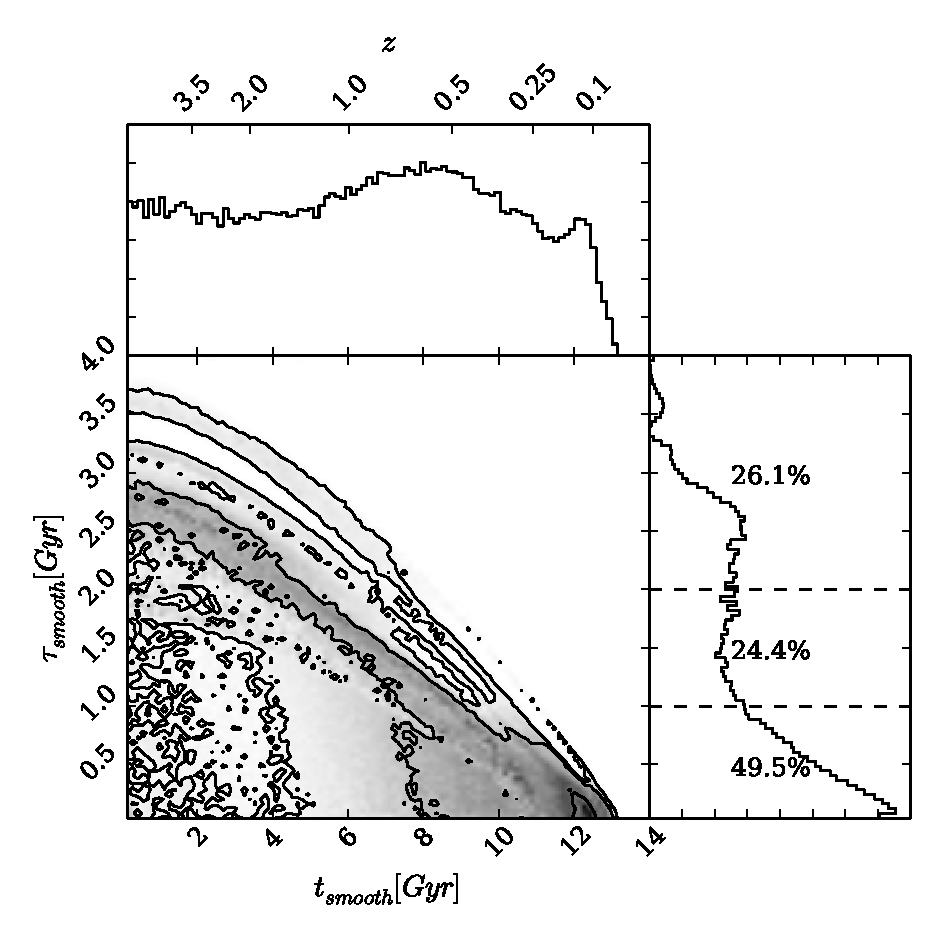
\includegraphics[width=0.55\textwidth]{morphology/red_smooth.pdf}\\
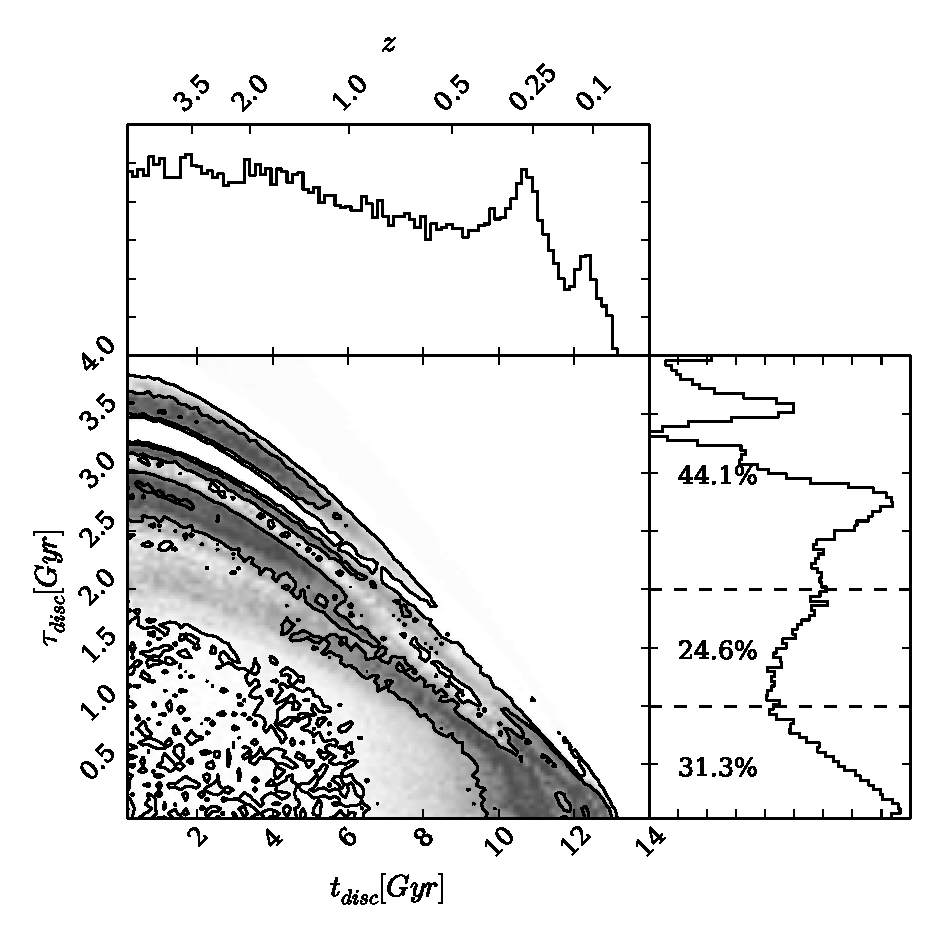
\includegraphics[width=0.55\textwidth]{morphology/red_disc.pdf}}
\caption[Population densities of red smooth and disc galaxies]{Contour plots showing the population densities for red galaxies of the \textsc{gz2-galex} sample, weighted by the morphological vote fractions from GZ2 to give both bulge (top) and disc (bottom) dominated distributions. The histograms show the projection into one dimension for each parameter. The dashed lines show the separation between rapid ($\tau ~\rm{[Gyr]} < 1.0$), intermediate ($1.0 < \tau ~\rm{[Gyr]} < 2.0$) and slow ($\tau ~\rm{[Gyr]} > 2.0$) quenching timescales with the fraction of the combined posterior probability distribution in each region shown (see Section~\ref{stats}).}
\label{red_s}
\end{figure*}

The top panel of Figure~\ref{red_s} reveals that the red smooth weighted population density is dominated $(49.5\%$; see Figure~\ref{red_s}) by rapid quenching timescales across all cosmic time resulting in a very low current SFR. At early quenching times (high redshift), the population density is dominated by slow and intermediate timescales (top panel of Figure~\ref{red_s}). Perhaps this is the influence of intermediate galaxies (with $p_s \sim p_d \sim 0.5$), hence why similar high density areas exist for both the smooth and disc weighted populations in the top and bottom panels of Figure~\ref{red_s}. This is especially apparent considering there are far more of these intermediate galaxies than those that are definitively early- or late-types (see Table~\ref{table:subs}). 

The bottom panel of Figure~\ref{red_s} reveals a bimodal disc weighted population density between rapid $(31.3\%)$ and slow $(44.1\%)$ quenching timescales. The \emph{very} slow ($\tau > 3.0 ~\rm{Gyr}$) quenching timescales present in these red disc population densities (which are not seen in either the green valley or blue cloud, see Figures~\ref{green_v} and~\ref{blue_c}) suggest that these galaxies have only just reached the red sequence after a very slow evolution across the colour-magnitude diagram. Considering their limited number and the requirement for NUV emission, it is likely that these galaxies are currently on the edge of the red sequence having recently (and finally) moved out of the green valley. 

Despite this dominance of slow quenching timescales in the red disc weighted population densities, rapid quenching timescales also contribute a significant fraction ($31.3\%$). This is similar to the red smooth weighted population, albeit with a marginally lower fraction of population density. 

\citet{tojeiro13} used the VErsatile SPectral Analyses spectral fitting code (VESPA; \citealt{tojeiro07}) and found that red late-type spirals show 17 times more recent star formation than red elliptical galaxies. The results in Figure \ref{red_s} can be tested against this finding  by comparing the SFRs predicted by the inferred SFH model of both the smooth and disc weighted population densities (these SFRs are shown in Figure \ref{pred}). For the peak at early times and slow quenching rate in the red disc weighted population density, this SFH model still has some residual star formation occurring with a SFR$~\sim0.105 M_{\odot}yr^{-1}$. Whereas the peak at recent times and rapid quenching rates in the red smooth weighted population density, this SFH model has a resultant SFR$~\sim0.0075 M_{\odot}yr^{-1}$. This is approximately 14 times less than the residual SFR still occurring in the red disc weighted population; within error, this is in agreement with the findings of \citet{tojeiro13}. 

These results for the red galaxies have many implications for green valley galaxies, as all of these systems must have passed through the green valley on their way to the red sequence.


\subsection{Green Valley Galaxies}\label{gv}

\begin{figure*}
\centering{
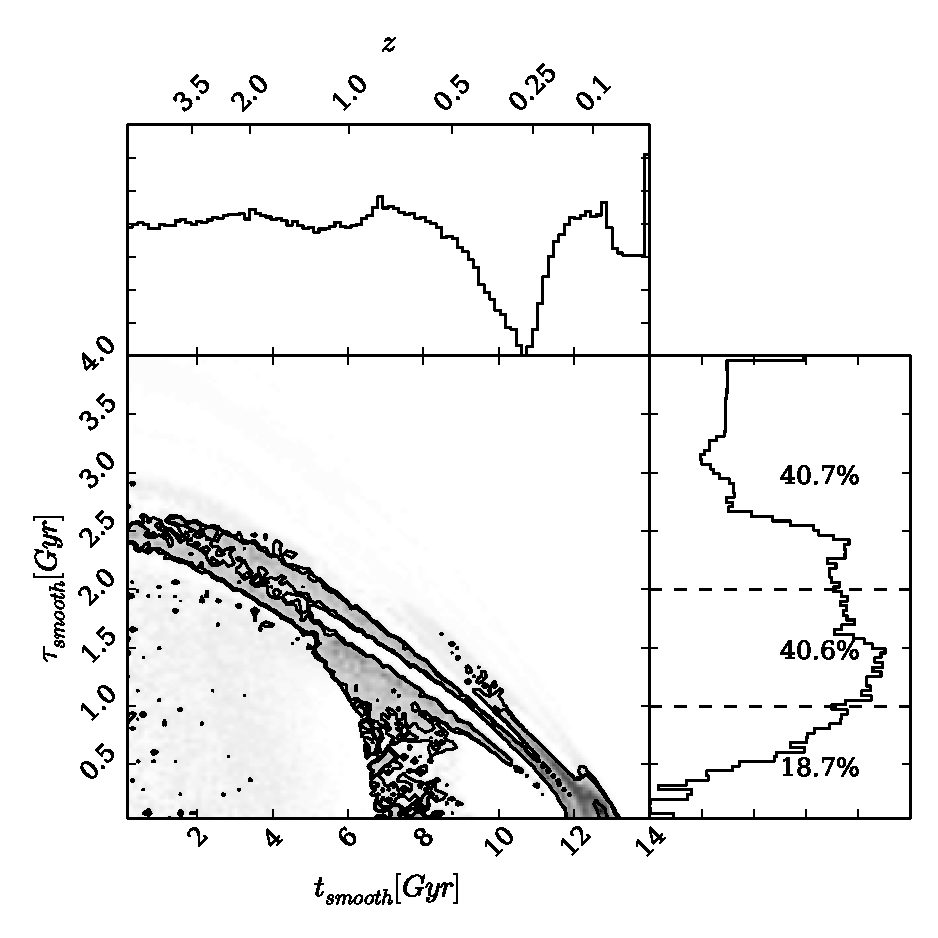
\includegraphics[width=0.55\textwidth]{morphology/green_smooth.pdf}\\
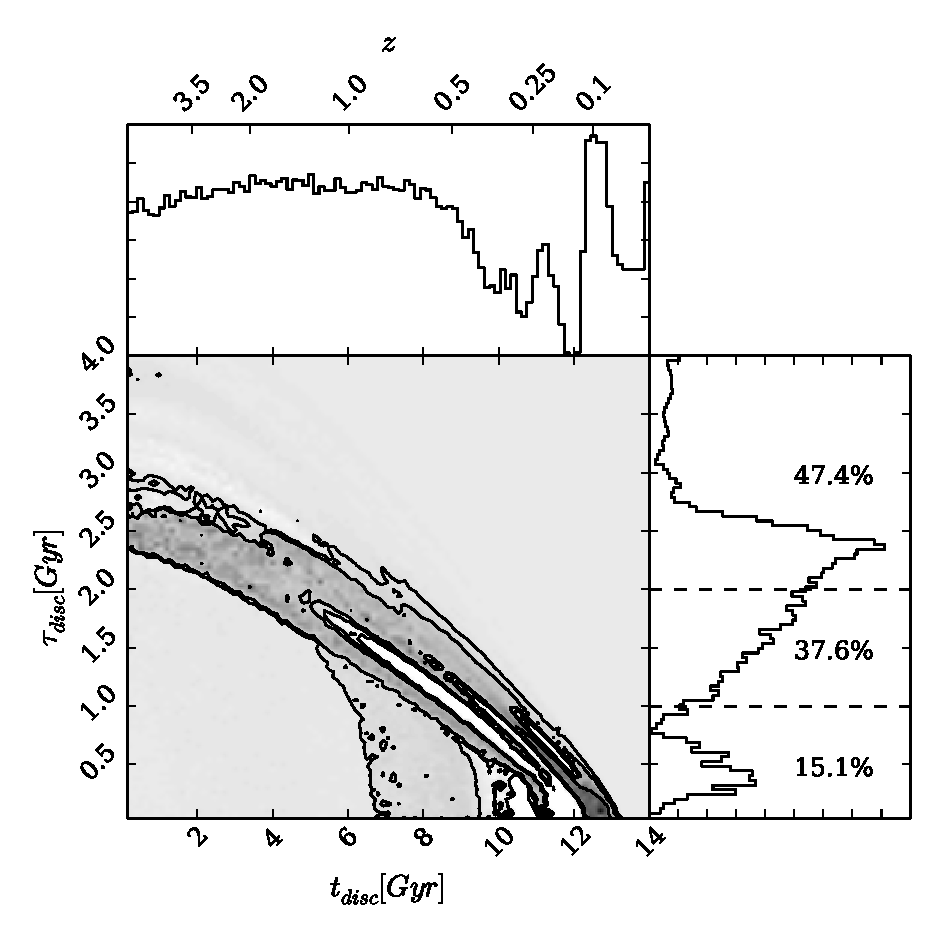
\includegraphics[width=0.55\textwidth]{morphology/green_disc.pdf}}
\caption[Population densities of green smooth and disc galaxies]{Contour plots showing the population densities for green valley galaxies in the \textsc{gz2-galex} sample weighted by the morphological vote fractions from GZ2 to give both bulge (top) and disc (bottom) dominated distributions. The histograms show the projection into one dimension for each parameter. The dashed lines show the separation between rapid ($\tau ~\rm{[Gyr]} < 1.0$), intermediate ($1.0 < \tau ~\rm{[Gyr]} < 2.0$) and slow ($\tau ~\rm{[Gyr]} > 2.0$) quenching timescales with the fraction of the combined posterior probability distribution in each region shown (see Section~\ref{stats}).}
\label{green_v}
\end{figure*}

Figure \ref{green_v} shows how the smooth weighted green valley population densities are dominated by both intermediate quenching rates ($40.6\%$) and slow quenching at rates early times ($z > 1$; $40.7\%$). The fraction of the population density at rapid quenching rates in the smooth weighted population has dropped by over a half compared to the red sequence smooth weighted population. However this will be influenced by the observability of galaxies in the green valley undergoing such a rapid quench. To quantify this, I tested the time spent in the green valley across the $[t, \tau]$ parameter space, which is shown in Figure~\ref{fig:timeingv}. The galaxies with such a rapid decline in star formation rate spend very little time in the green valley and so will be detected at a lower fraction than those galaxies transitioning more slowly with intermediate quenching rates.  This explains the observed number of intermediate morphology galaxies (see Table \ref{table:subs}) which are present in the green valley (assuming a morphological change occurs during the quench) and explains the dominance of rapid quenching rates in the red smooth and disc weighted population densities (see Figure \ref{red_s}).

\begin{figure*}
\centering{
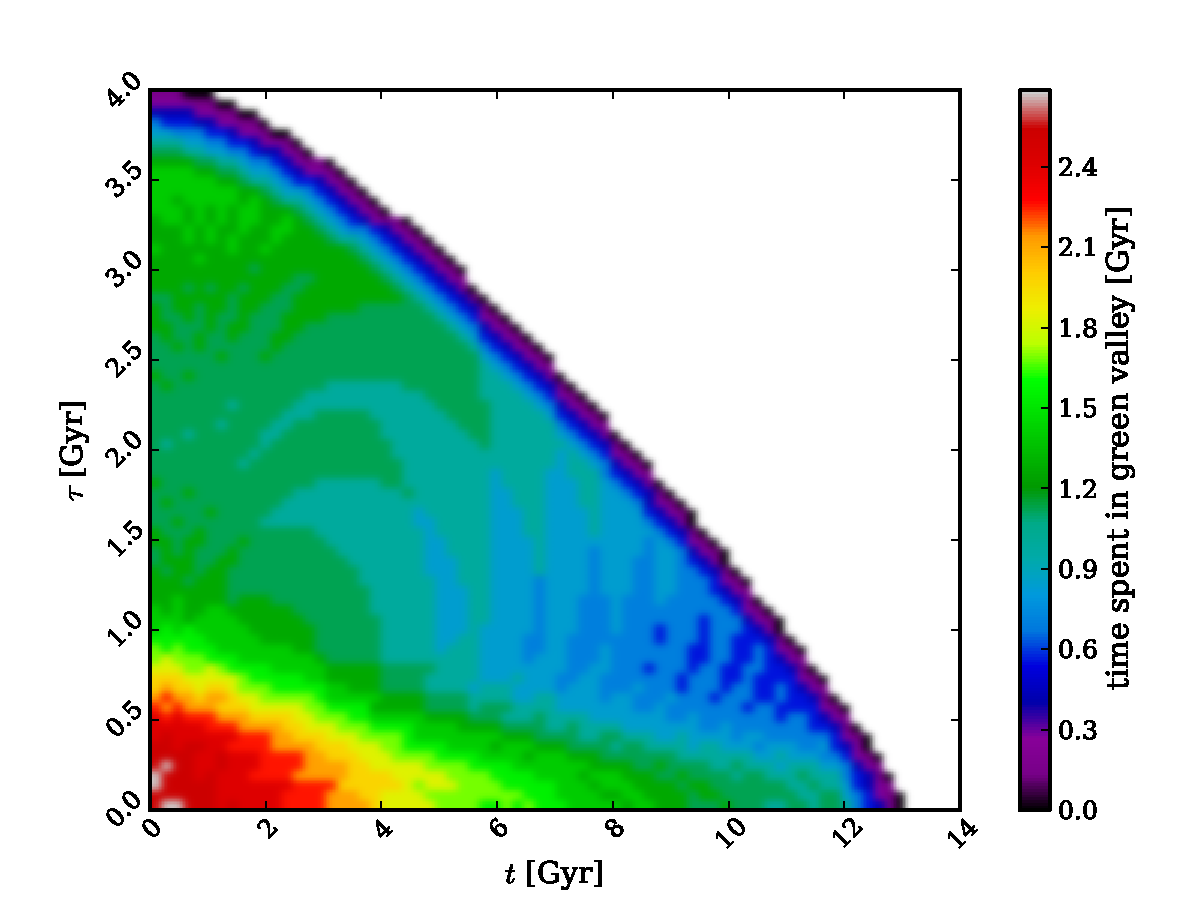
\includegraphics[width=0.9\textwidth]{morphology/green_valley_time.pdf}}
\caption[Time spent in the green valley across parameter space]{Plot showing the time spent in the green valley across the SFH model parameter space by the current epoch. This affects the observability of those galaxies which have quenched rapidly and recently and have passed too quickly through the green valley to be detected. The white region denotes those models with colours that do not enter the green valley by the present cosmic time.}
\label{fig:timeingv}
\end{figure*}

Conversely, the green valley disc weighted population densities are now completely dominated by slow quenching rates ($47.4\%$) with a slightly smaller fraction of intermediate quenching rates detected ($37.6\%$; see Figure~\ref{green_v}).

If the population densities of Figure~\ref{green_v} and Figure~\ref{red_s} are compared, quenching is detected at later cosmic times (lower redshift) in the green valley than in the red sequence for both morphological types. This therefore suggests that both morphologies are tracing the evolution of the red sequence, confirming that the green valley is indeed a transitional population between blue cloud and red sequence regardless of morphology. 

Given enough time ($t\sim4 - 5~\rm{Gyr}$), the current green valley disc galaxies will therefore eventually transition through to the red sequence (the right panel of Figure~\ref{sfr_mass_col} shows galaxies with $\tau > 1.0~\rm{Gyr}$ do not approach the red sequence within $3~\rm{Gyr}$ post quench). This is most likely the origin of the `red spirals', attributed to the \emph{very} slow quenching rates discussed in Section~\ref{rs} (and see bottom panel of Figure~\ref{red_s}). This is in contradiction to the conclusions of S14 who state that the green valley disc population is static in nature. 

Considering this result that the green valley is a transitional population, the ratio of smooth:disc galaxies that is currently observed in the green valley is expected to evolve into the ratio observed in the red sequence (assuming that the decreased number of galaxies detected in the red sequence due to matching to GALEX is independent of morphology). Table~\ref{table:subs} shows the ratio of smooth-like : disc-like galaxies in the red sequence is $62:38$, whereas in the green valley this ratio is $45:55$. Making the very simple assumptions that this ratio does not change with redshift and that quenching is the only mechanism which causes a morphological transformation, then $31.2\%$ of the disc-like galaxies in the green valley would have to undergo a morphological change to a smooth-like galaxy. 

Inspecting the the disc weighted green valley population density (bottom panel of Figure~\ref{green_v}) reveals that $29.4\%$ of the distribution occupies the $\tau < 1.5 ~\rm{Gyr}$ parameter space. Since this is a similar fraction to the number of green valley disc-like galaxies which would have to undergo a morphological change to a smooth-like galaxy to match the ratio of smooth:disc galaxies in the red sequence, this suggests that quenching mechanisms with $\tau < 1.5 ~\rm{Gyr}$ are capable of destroying the disc-dominated structure of galaxies. 

However this is most likely an overestimate of the timescale that can cause a morphological change because of the observability of those galaxies which undergo such a rapid quench. \citet{Martin07} showed that after considering the time spent in the green valley, the fraction of galaxies inferred to be undergoing a rapid quench would quadruple. If this result is applied to the disc weighted green valley population density (bottom panel Figure~\ref{green_v}) and the distribution was then renormalised, the resulting population density would be very similar in shape to the one found for the disc weighted red sequence population (bottom panel Figure~\ref{red_s}). This provides more evidence that the green valley is tracing the evolution of the red sequence and is therefore a transitional population.

All of this evidence suggests that there are not just two contrasting evolutionary pathways through the green valley for different morphological types as concluded by S14. The intermediate quenching rates reside in the space between the extremes sampled by the optical-NUV colour-colour diagrams of S14. The inclusion of the intermediate galaxies in this investigation and the use of a statistical method, elucidates a continuum of quenching timescales, with all galaxies transitioning through the green valley to the red sequence during quenching regardless of morphology. 

Instead of concluding that \emph{`the green valley is a red herring'} as in S14, I would therefore conclude that the \emph{`grass is always redder on the other side'}.


\subsection{Blue Cloud Galaxies}\label{bc}

\begin{figure*}
\centering{
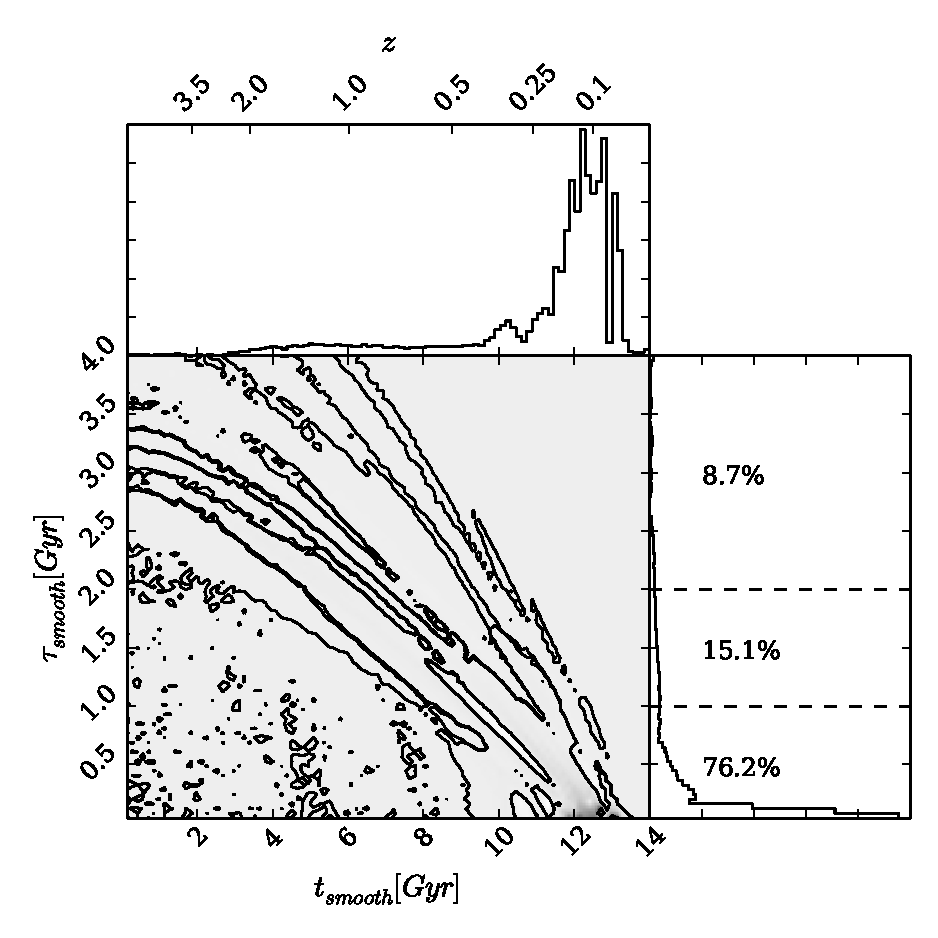
\includegraphics[width=0.55\textwidth]{morphology/blue_smooth.pdf}\\
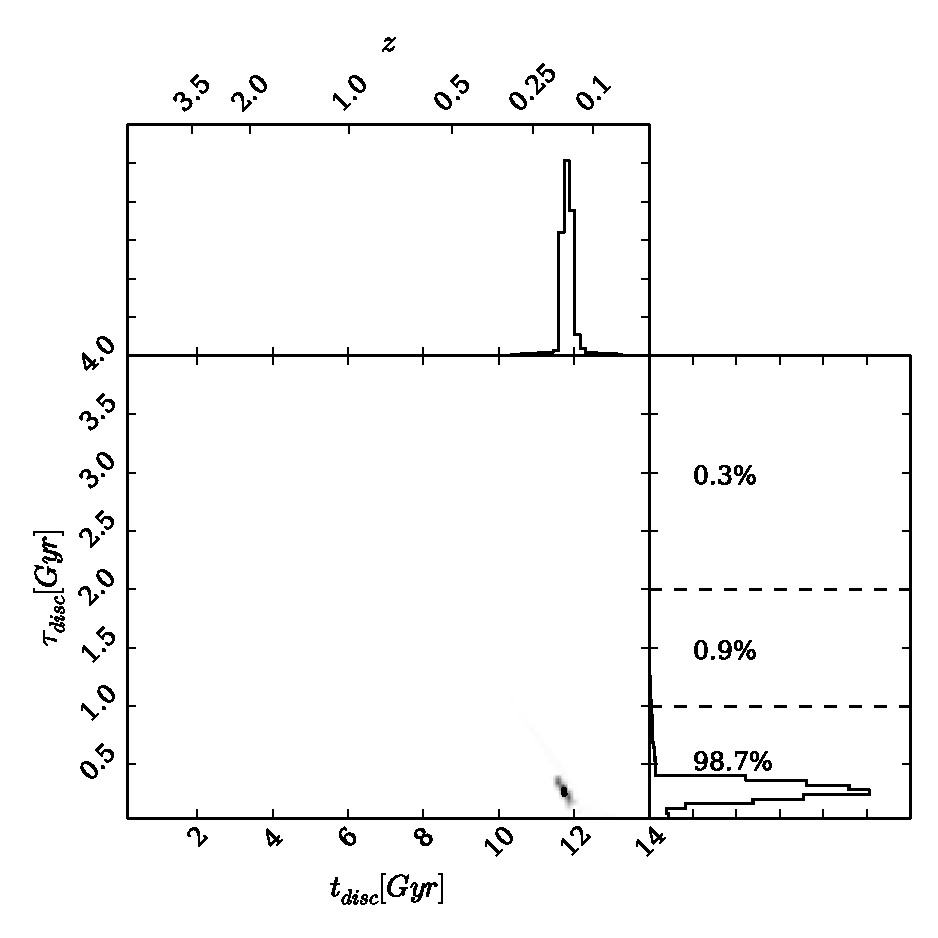
\includegraphics[width=0.55\textwidth]{morphology/blue_disc.pdf}}
\caption[Population densities of blue smooth and disc galaxies]{Contour plots showing the population densities blue cloud galaxies in the \textsc{gz2-galex} sample, weighted by the morphological vote fractions from GZ2 to give both bulge (top) and disc (bottom) dominated distributions. The histograms show the projection into one dimension for each parameter. The dashed lines show the separation between rapid ($\tau ~\rm{[Gyr]} < 1.0$), intermediate ($1.0 < \tau ~\rm{[Gyr]} < 2.0$) and slow ($\tau ~\rm{[Gyr]} > 2.0$) quenching timescales with the fraction of the combined posterior probability distribution in each region shown (see Section~\ref{stats}). Positions with probabilities less than 0.2 are discarded as poorly fit models, therefore unsurprisingly blue cloud galaxies are not well described by a quenching star formation model. }
\label{blue_c}
\end{figure*}

\begin{figure*}
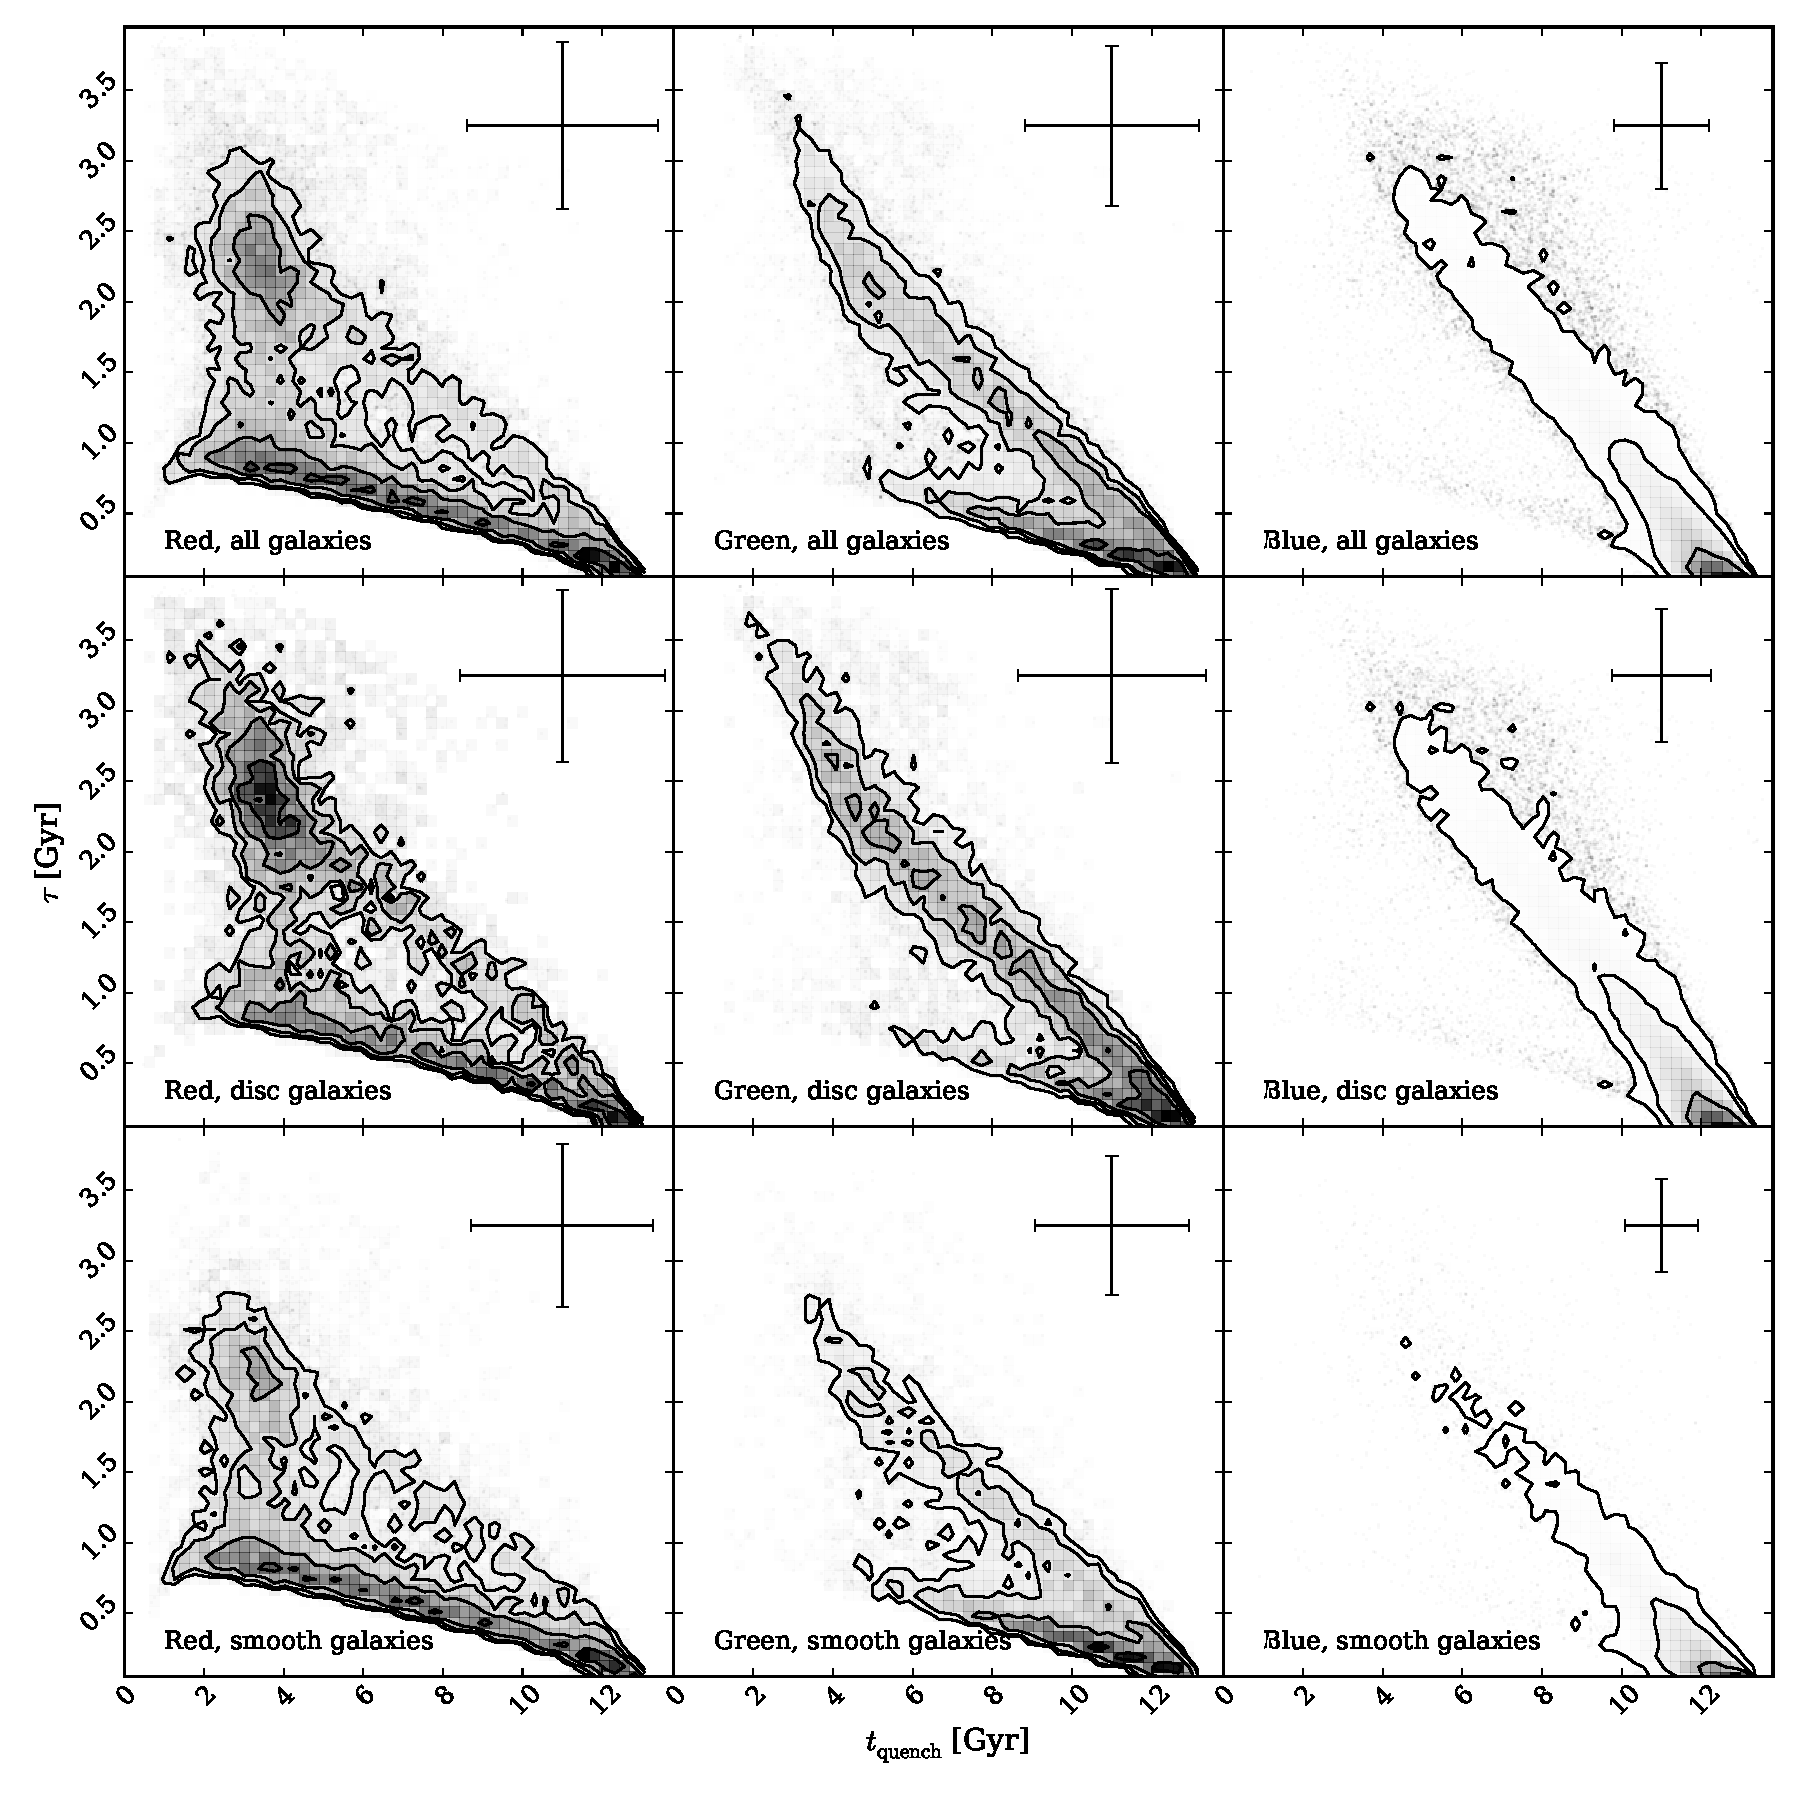
\includegraphics[width=0.95\textwidth]{morphology/contour_t_tau_mcmc_bestfit.pdf}
\caption[Best fit contours for red, green and blue clean galaxies]{Contours showing the positions in the $[t, \tau]$ parameter space of the median walker position (the 50th percentile; as shown by the intersection of the solid blue lines in Figure~\ref{one_example}) for each galaxy for all (top), disc ($p_d > 0.5$; middle), and smooth ($p_s > 0.5$; bottom) red sequence, green valley and blue cloud galaxies in the left, middle and bottom panels respectively. The error bars on each panel shows the average $68\%$ confidence on the median positions (calculated from the 16th and 84th percentile, as shown by the blue dashed lines in Figure~\ref{one_example}). These positions were calculated without discarding any walker positions due to low probability and without weighting by vote fractions, therefore this plot may be more intuitive than Figures~\ref{red_s},~\ref{green_v} \&~\ref{blue_c}. The differences between the smooth and disc populations and between the red, green and blue populations remain clearly apparent.}
\label{fig:bestfit}
\end{figure*}

Since the blue cloud is considered to be made of star forming galaxies \starpy~ is expected to have some difficulty inferring any quenching model to describe them, as confirmed by Figure~\ref{blue_c}. The attempt to characterise a star forming galaxy with a quenched SFH model leads \starpy~ to attribute the extremely blue colours of the majority of these galaxies with a constant SFR until recent times with a fast quench at the observed redshift (i.e. the colour has not had enough time to change from blue post-quench). 

This is particularly apparent for the blue disc weighted population. Perhaps even galaxies which are currently quenching slowly across the blue cloud cannot be well fit by the quenching models implemented, as they still have high SFRs despite some quenching. By definition although a galaxy is undergoing quenching, star formation can still be occurring in a galaxy, just at a slower rate than at earlier times, described by $\tau$.

A very small fraction of the blue smooth weighted population density is found at slower quenching rates which began prior to $z \sim 0.5 $. These populations have been blue for a considerable period of time, slowly using up their gas for star formation by the Kennicutt$-$Schmidt law \citep{Schmidt59, Kennicutt97}. However the dominant fraction of the blue smooth weighted population density occurs at rapid quenching rates at recent times. This therefore provides some support to the theories for blue ellipticals as either merger-driven ($\sim76\%$; like those identified as recently quenched ellipticals with properties consistent with a merger origin by \citealt{McIntosh14}) or gas inflow-driven reinvigorated star formation that is now slowly decreasing ($\sim24\%$; such as the population of blue spheroidal galaxies studied by \citealt{Kaviraj13}).

The blue cloud is therefore primarily composed of both star forming galaxies of all morphologies and a smooth population which are undergoing a rapid quench, presumably after a previous event triggered star formation and turned them blue.


\section{Discussion}\label{morph:discussion}

In the previous section I presented the results of using \textsc{popstarpy} to derive the distribution of quenching histories for galaxies across the colour magnitude diagram. I  found differences between the SFHs of smooth- and disc-weighted populations of the red sequence, green valley and blue cloud. These results are summarised in Table~\ref{table:morphresults}. In this section I will speculate on the following question: what are the possible mechanisms driving these differences? 

\begin{table}[]
\centering
\caption{Table summarising the main results in Section~\ref{results} by describing the distributions derived for each population across the colour-magnitude diagram.}
\label{table:morphresults}
\resizebox{\textwidth}{!}{%
\begin{tabular}{rccc}
\hline
                                     & Red Sequence                                                                                 & Green Valley                                                                            & Blue Cloud                                                                       \\ \hline \hline
\multicolumn{1}{r|}{Smooth-weighted} & \begin{tabular}[c]{@{}c@{}}Dominated by \\ rapid \\ quenching rates\end{tabular}             & \begin{tabular}[c]{@{}c@{}}Dominated by \\ intermediate \\ quenching rates\end{tabular} & \begin{tabular}[c]{@{}c@{}}Dominated by \\ rapid \\ quenching rates\end{tabular} \\ \hline
\multicolumn{1}{r|}{Disc-weighted}   & \begin{tabular}[c]{@{}c@{}}Bimodal between \\ slow and rapid \\ quenching rates\end{tabular} & \begin{tabular}[c]{@{}c@{}}Dominated by \\ slow \\ quenching rates\end{tabular}         & -                                                                                \\ \hline
\end{tabular}%
}
\end{table}

\subsection{Rapid Quenching Mechanisms}\label{rapid}

Rapid quenching is found at larger fractions in the smooth weighted population densities than the disc weighted. Red galaxies also have larger fractions of raid quenching rates than green valley population densities. However the observability of a galaxy may decline with increasing quenching rate. Rapid mechanisms may be more common in the green valley than found in Figure \ref{green_v}, however this observability should not depend on morphology. The conclusion that rapid quenching mechanisms are detected more for smooth rather than disc populations still holds. 

This suggests that rapid quenching mechanisms can cause a change in morphology from a disc- to a smooth dominated galaxy as it quickly traverses the colour-magnitude diagram to the red sequence. This is supported by the number of disc galaxies that would need to undergo a morphological change in order for the disc : smooth ratio of galaxies in the green valley to match that of the red sequence (see Section~\ref{gv}). From this indirect evidence I suggest that this observed rapid quenching mechanism is caused by major mergers. However, since a significant fraction of the red disc weighted population density is found at rapid quenching rates, this suggests that the quenching may have occurred more rapidly than the morphological change in such a merger.

Inspection of the individual galaxies dominating this area of the smooth weighted red population density reveals that this dominance of rapid quenching not arise due to \emph{currently} merging galaxies. Although efforts were made to remove currently merging galaxies from the \textsc{gz2-galex} sample (using the GZ2 morphological vote fractions, see Section \ref{class}), this check was still performed to ensure no merging pairs were missed by the GZ users. Instead, the area is dominated by typical smooth galaxies with both red optical and NUV colours that \starpy~ attributes to rapid quenching at early times. Although a prescription for modelling a merger in the SFH is not included in this work the after-effects can still be detected (see Section \ref{future} for future work planned with \starpy).

In order to achieve such rapid quenching rates ($\tau \lesssim 0.5$) in a simulation of a major merger, \citet*{springel05} showed that feedback from black hole activity is necessary. As discussed in Section \ref{intro}, powerful quasar outflows are thought to be able to remove much of the gas from the inner regions of the galaxy, terminating star formation on extremely short timescales. \citet{Bell06}, using data from the COMBO-17 redshift survey ($0.4 < z < 0.8$), estimate a merger timescale of $\sim 0.4~\rm{Gyr}$ for the merger to go from being classified as a close galaxy pair to morphologically disturbed. \citet*{springel05b} consequently find using hydrodynamical simulations that after $\sim1~\rm{Gyr}$ the merger remnant has reddened to $u-r \sim 2.0$. This is in agreement with the simple exponential quenching models used here which show (Figure~\ref{sfr_mass_col}) that the models with a SFH with $\tau < 0.4~\rm{Gyr}$ have reached the red sequence, with $u-r ~\gtrsim 2.2$, within $\sim1~\rm{Gyr}$. This could explain the preference for red disc galaxies with rapid quenching timescales ($31.3\%$), as they may have undergone a major merger recently but are still undergoing a morphological change from disc, to disturbed, to an eventual smooth galaxy (see also \citealt{vdW09}) or have retained their disc structure in a merger in line with recent simulations from \citet{pontzen16}. This possible connection between AGN feedback and rapid quenching timescales is explored further in Chapter~\ref{agnfeedback}. 

This rapid quenching mechanism occurs much more rarely in green valley galaxies of both morphologies than for the subset of red sequence galaxies studied, however does not fully characterise all the galaxies in either the red sequence or green valley. Dry major mergers therefore do not fully account for the formation of any galaxy type at any redshift, supporting the observational conclusions made by \citet{Bell07,Bundy07, kaviraj14a} and simulations by \citet{Genel08}. 

\subsection{Intermediate Quenching Mechanisms}\label{int}

Intermediate quenching timescales are found to be equally prevalent across  all populations of both smooth and disc galaxies across cosmic time,  particularly in the green valley. Intermediate timescales are the prevalent mechanism for quenching smooth green valley galaxies, unlike the rapid quenching prevalent for red galaxies. This suggests that this intermediate quenching route must therefore be possible with routes that both preserve and transform morphology. It is this result of another route through the green valley that is in contradiction with the findings of S14. 

Once again considering the simulations of \citet{springel05b}, this time without any feedback from black holes, they suggest that if even a small fraction of gas is not consumed in the starburst following a merger (either because the mass ratio is not large enough or from the lack of strong black hole activity) the remnant can sustain star formation for periods of several Gyrs. The remnants from these simulations take $\sim5.5~\rm{Gyr}$ to reach red optical colours of $u-r \sim 2.1$. In Figure~\ref{sfr_mass_col} it can be seen that the models with intermediate quenching timescales of $1.0 \lesssim ~\tau~\rm{[Gyr]} ~\lesssim 2.0$ take approximately $2.5-5.5~\rm{Gyr}$ to reach these red colours. Similarly the recent simulations of \citet{pontzen16} show that without feedback the SFR of a disc galaxy can recover post merger and remain a star forming disc. 

I propose that the intermediate quenching timescales are caused by gas rich major mergers, major mergers without black hole feedback and from minor mergers, the latter of which being the dominant mechanism. This is supported by the findings of \citet{lotz08b} who find that the detectability timescales for equal mass gas rich mergers with large initial separations range from $\sim 1.1-1.9~\rm{Gyr}$, and of \citet{Lotz11}, who find in further simulations that as the baryonic gas fraction in a merger with mass ratios of 1:1-1:4 increases, so does the timescale of the merger from $\sim0.2~\rm{Gyr}$ (with little gas, as above for major mergers causing rapid quenching timescales) up to $\sim1.5~\rm{Gyr}$ (with large gas fractions). 

Here the very basic assumption is that the morphologically detectable timescale of a merger is roughly the same order as the quenching timescale. However, the existence of a substantial population of blue ellipticals \citep{Sch09} must be considered, which are thought to be post-merger systems with no detectable morphological signatures of a merger but with the merger-induced starburst still detectable in the photometry. This photometry is an indicator for the SFH and therefore should present with longer timescales for the photometric effects of a merger than found in the simulations by \citet{lotz08b} and \citet{Lotz11}. Observing this link between the timescale for the morphological observability of a merger and the timescales for the star formation induced by a merger is problematic, as evidenced by the lack of literature on the subject.

\citet{lotz08b} also show that the remnants of these simulated equal mass gas rich disc mergers (wet disc mergers) are observable for $\gtrsim1~\rm{Gyr}$ post merger and state that they appear ``disc-like and dusty" in the simulations, which is consistent with an ``early-type spiral morphology".  Such galaxies are often observed to have spiral features with a dominant bulge, suggesting that such galaxies may divide the votes of the GZ2 users, producing vote fractions of $p_s \sim p_d \sim 0.5$. This may be why the intermediate quenching timescales are equally dominant for both smooth and disc populations in Figures~\ref{red_s} and~\ref{green_v}. 

Other simulations (e.g. such as \citet{robertson06} and \citet{Barnes02}) support the conclusion that both gas rich major mergers and minor mergers can produce disc-like remnants. Observationally, \citet{Darg10a} showed an increase in the spiral to elliptical ratio for merging galaxies ($0.005 < z < 0.1$) by a factor of two compared to the general population. They attribute this to the much longer timescales during which mergers of spirals are observable compared to mergers with elliptical galaxies, confirming the hypothesis that the quenching timescales $\tau < 1.5 ~\rm{Gyr}$ preferred by disc galaxies may be undergoing mergers which will eventually lead to a morphological change. Similarly, \citet{Casteels13} observe that galaxies ($0.01 < z < 0.09$) which are interacting often retain their spiral structures and that a spiral galaxy which has been classified as having `loose winding arms' by the GZ2 users are often entering the early stages of mergers and interactions.

$40.6\%$ of the probability for smooth galaxies in the green valley arises due to intermediate quenching timescales (see Figure~\ref{green_v}); this is in agreement with work done by \citet{kaviraj14a, kaviraj14b} who by studying SDSS photometry ($z<0.07$) state that approximately half of the star formation in galaxies is driven by minor mergers at $0.5 < z < 0.7$ therefore exhausting available gas for star formation and consequently causing a gradual decline in the star formation rate. This supports earlier work by \cite{kaviraj11} who, using multi wavelength photometry of galaxies in COSMOS \citep{Scoville07}, found that $70\%$ of early-type galaxies appear morphologically disturbed, suggesting either a minor or major merger in their history. This is in agreement with the total percentage of the population density with $\tau < 2.0 ~\rm[Gyr]$; $73.9\%$ and $59.3\%$, for the smooth red and green galaxies in Figures~\ref{red_s} and~\ref{green_v} respectively. Note that the star formation model used here is a basic one and has no prescription for reignition of star formation post-quench which can also cause morphological disturbance of a galaxy, like those detected by \cite{kaviraj11} and seen in simulations by \cite{pontzen16}.

\citet{Darg10a} show in their Figure 6 that that beyond a merger ratio of $1:10$ (up to $\sim 1:100$), green is the dominant average galaxy colour of the visually identified merging pair in GZ. These mergers are also dominated by spiral-spiral mergers as opposed to elliptical-elliptical and elliptical-spiral. This supports the hypothesis that these intermediate timescales dominating in the green valley are caused in part by minor mergers. However this is contradictory to the findings of \citet{Mendez11} who find the merger fraction in the green valley is much lower than in the blue cloud, however they use an analytical light decomposition indicator to identify their mergers ($Gini/M_{20}$; see \citealt{lotz08b}), which tends to detect major mergers more easily than minor mergers. I have discussed the lower likelihood of a green valley galaxy to undergo a rapid quench, which I have hypothesised are attributed to major mergers (see Section \ref{rapid}), despite the caveat of the observability and believe that this may have been the phenomenon that \citet{Mendez11} detected.

The resultant intermediate quenching timescales occur initially due to one interaction mechanism, unlike the rapid quenching, which occurs due to a major merger combined with AGN feedback, and decreases the SFR over a short period of time. Therefore any external event which can cause either a burst of star formation (depleting the gas available) or directly strip a galaxy of its gas, for example galaxy harassment, interactions, ram pressure stripping, strangulation and interactions internal to clusters, would cause quenching on an intermediate timescale. Such mechanisms would be the dominant cause of quenching in dense environments; considering that the majority of galaxies reside in groups or clusters (\citealt{Coil08} find that green valley galaxies are just as clustered as red sequence galaxies). It is not surprising therefore that the majority of the \textsc{gz2-galex} galaxies are considered intermediate in morphology (see Table~\ref{table:subs}) and therefore are undergoing or have undergone such an interaction. This obvious dependancy of the quenching parameters with the galaxy environment will be investigated further in Chapter~\ref{chap:env}.

These galaxies are those whose morphology cannot be easily distinguished either because they are at a large distance or because they are an S0 galaxy whose morphology can be interpreted by different GZ2 users in different ways. \citet{GZ2} find that S0 galaxies expertly classified by \citet{nair10} are more commonly classified as ellipticals by GZ2 users, but have a significant tail to high disc vote fractions, giving a possible explanation as to the origin of this area of probability.


\subsection{Slow Quenching Timescales}\label{slow}
Although intermediate and rapid quenching timescales are the dominant mechanisms across the colour-magnitude diagram, together they cannot completely account for the quenching of disc galaxies. S14 concluded that slow quenching timescales were the most dominant mechanism for disc galaxies. However I show that: (i) intermediate quenching timescales are equally important in the green valley and (ii) rapid quenching timescales are equally important for the red galaxies with NUV emission. There is also a significantly lower preference for smooth galaxies to undergo such slow quenching timescales; suggesting that the evolution (or indeed creation) of typical smooth galaxies is dominated by processes external to the galaxy. This is excepting galaxies in the blue cloud where a small amount of slow evolution of blue ellipticals is occurring, presumably after a reinvigoration of star formation which is slowly depleting the gas available according to the Kennicutt$-$Schmidt law.

\citet{Bamford09} using GZ1 vote fractions of galaxies in the SDSS, found a significant fraction of high stellar mass red spiral galaxies in the field. As these galaxies are isolated from the effects of interactions from other galaxies, the slow quenching mechanisms present in their preferred star formation histories are most likely due to secular processes (i.e. mechanisms internal to the galaxy, in the absence of sudden accretion or merger events; \citealt{kormendy04, Sheth12}). Bar formation in a disc galaxy is such a mechanism, whereby gas is funnelled to the centre of the galaxy by the bar over long timescales where it is used for star formation \citep{masters12a, saintonge12, Cheung13}, consequently forming a `pseudo-bulge' \citep{Kormendy10, Simmons13}.

Table~\ref{table:subs} shows that $3.9\%$ of the sample are red sequence late-type galaxies, i.e. red late-type spirals. This is, within uncertainties, in agreement with the findings of \citet{masters10c}, who find $\sim6\%$ of late-type spirals are red when defined by a cut in the $g-r$ optical colour (rather than with $u-r$ as used in this investigation) and are at the `blue end of the red sequence'. 

If these slow quenching timescales are due to secular evolution processes, this is to be expected since these processes do not change the disc dominated nature of a galaxy. 

\section{Conclusions}\label{morph:conc}

I have used morphological classifications from the Galaxy Zoo 2 project to determine the morphology-dependent star formation histories of galaxies via a Bayesian analysis of an exponentially declining star formation quenching model. The most likely parameters were determined for the quenching onset time, $t_q$ and quenching timescale $\tau$ in this model for galaxies across the blue cloud, green valley and red sequence to trace the morphological dependance of galactic evolution across the colour-magnitude diagram. The green valley is indeed found to be a transitional population for all morphological types (in agreement with \citet{schawinski14}), however this transition proceeds slowly for the majority of disc dominated galaxies and occurs rapidly for the majority of smooth dominated galaxies in the red sequence. However, in addition to \citet{schawinski14}, this Bayesian approach has revealed a more nuanced result, specifically that the prevailing mechanism across all morphologies and populations is quenching with intermediate timescales. The main findings are summarised as follows:
\begin{enumerate}[(i)]
\item The subset of red sequence galaxies with NUV emission studied in this investigation are found to have similar preferences for quenching timescales compared to green valley galaxies, but the quenching occurs at earlier quenching times (i.e. higher redshift) regardless of morphology (see Figures~\ref{red_s} and~\ref{green_v}). Therefore the quenching mechanisms currently occurring in the green valley were also active in creating the `blue end of of the red sequence' at earlier times; confirming that the green valley is indeed a transitional population, regardless of morphology.

\item The typical red galaxy with NUV emission studied, is elliptical in morphology and has undergone a rapid to intermediate quench at some point in cosmic time, resulting in a very low current SFR (see Section~\ref{rs}.

\item The green valley as it is currently observed is dominated by very slowly evolving disc dominated galaxies along with intermediate- and smooth dominated galaxies which pass across it with intermediate timescales within $\sim 1.0-1.5~\rm{Gyr}$ (see Section~\ref{gv}).

\item There are many different mechanisms responsible for quenching, all causing a galaxy to progress through the green valley, which are dependant on galaxy type, with the smooth and disc dominated galaxies each having different dominant star formation histories across the colour-magnitude diagram. These timescales can be roughly split into three main regimes; rapid ($\tau < 1.0~$Gyr), intermediate ($1.0 < \tau~$[Gyr]~$< 2.0$) and slow ($\tau > 2.0~$ Gyr) quenching.

\item Blue cloud galaxies are not well fit by a quenching model of star formation due to the continuous high star formation rates occurring (see Figure~\ref{blue_c}).

\item Rapid quenching timescales are detected with a lower probability for green valley galaxies than the red sequence galaxies studied. I speculate that this quenching mechanism is caused by major mergers with black hole feedback, which are able to expel the remaining gas not initially exhausted in the merger-induced starburst and which can cause a change in morphology from disc- to bulge-dominated. The colour-change timescales from previous simulations of such events agree with the derived timescales (see Section~\ref{rapid}). These rapid timescales are instrumental in forming red galaxies, however galaxies at the current epoch passing through the green valley do so at more intermediate timescales (see Figure~\ref{green_v}).

\item Intermediate quenching timescales ($1.0 < ~\tau~\rm{[Gyr]}~ < 2.0 $) are found with constant density across red and green galaxies for both smooth- and disc-weighted populations, the timescales for which agree with observed and simulated minor merger timescales (see Section~\ref{int}). I hypothesise that such timescales can be caused by a number of external processes, including gas rich major mergers, mergers without black hole feedback, galaxy harassment, interactions and ram pressure stripping. The timescales and observed morphologies from previous studies agree with the results, including that this is the dominant mechanisms for intermediate galaxies such as early-type spiral galaxies with spiral features but a dominant bulge, which split the GZ2 vote fractions (see Section~\ref{int}). 

\item Slow quenching timescales are the most dominant mechanism in the disc galaxy populations across the colour-magnitude diagram. Disc galaxies are often found in the field, therefore I hypothesise that such slow quenching timescales are caused by secular evolution and processes internal to the galaxy (see Section \ref{bc}). A small amount of slow quenching timescales is also detected for blue elliptical galaxies which is attributed to a reinvigoration of star formation, the peak of which has passed and has started to decline by slowly depleting the gas available (see Section~\ref{bc}). 
\end{enumerate}


\chapter{Black hole-galaxy co-evolution in the context of quenching}\label{agnfeedback}

The following chapter is split into two parts; in Section \ref{agnfeedback} I investigate the connection between quenching parameters and the presence of an AGN and in Section \ref{intbulgeless} investigate how black holes grow in disc galaxies with merger free evolutionary histories. 

\section{Rapid, recent quenching within a population of Type 2 AGN host galaxies}\label{agnfeedback}

\emph{The work in the following chapter has been published in \citet{smethurst16}.}

In Chapter \ref{morph}, rapid quenching rates were dominant across the smooth weighted population densities in Figures~\ref{green_v} \& \ref{red_s}. In Section~\ref{rapid} I discussed how simulations suggest that such rapid quenching rates can only be achieved if AGN feedback is present in a major merger scenario. I therefore decided to investigate this possible connection between AGN feedback and rapid quenching rates further. I shall do so by analysing the SFHs of a population of AGN host galaxies with \textsc{popstarpy} in comparison to an inactive galaxy control sample. I  aim to determine the following: (i) Are galaxies currently hosting an AGN undergoing quenching? (ii) If so, when and at what rate does this quenching occur? (iii) Is this quenching occurring at different times and rates compared to a control sample of inactive galaxies? This builds on the work of \citet{Martin07} but improves significantly on previous techniques.

\subsection{AGN Sample}\label{agnsample}

\begin{figure*}
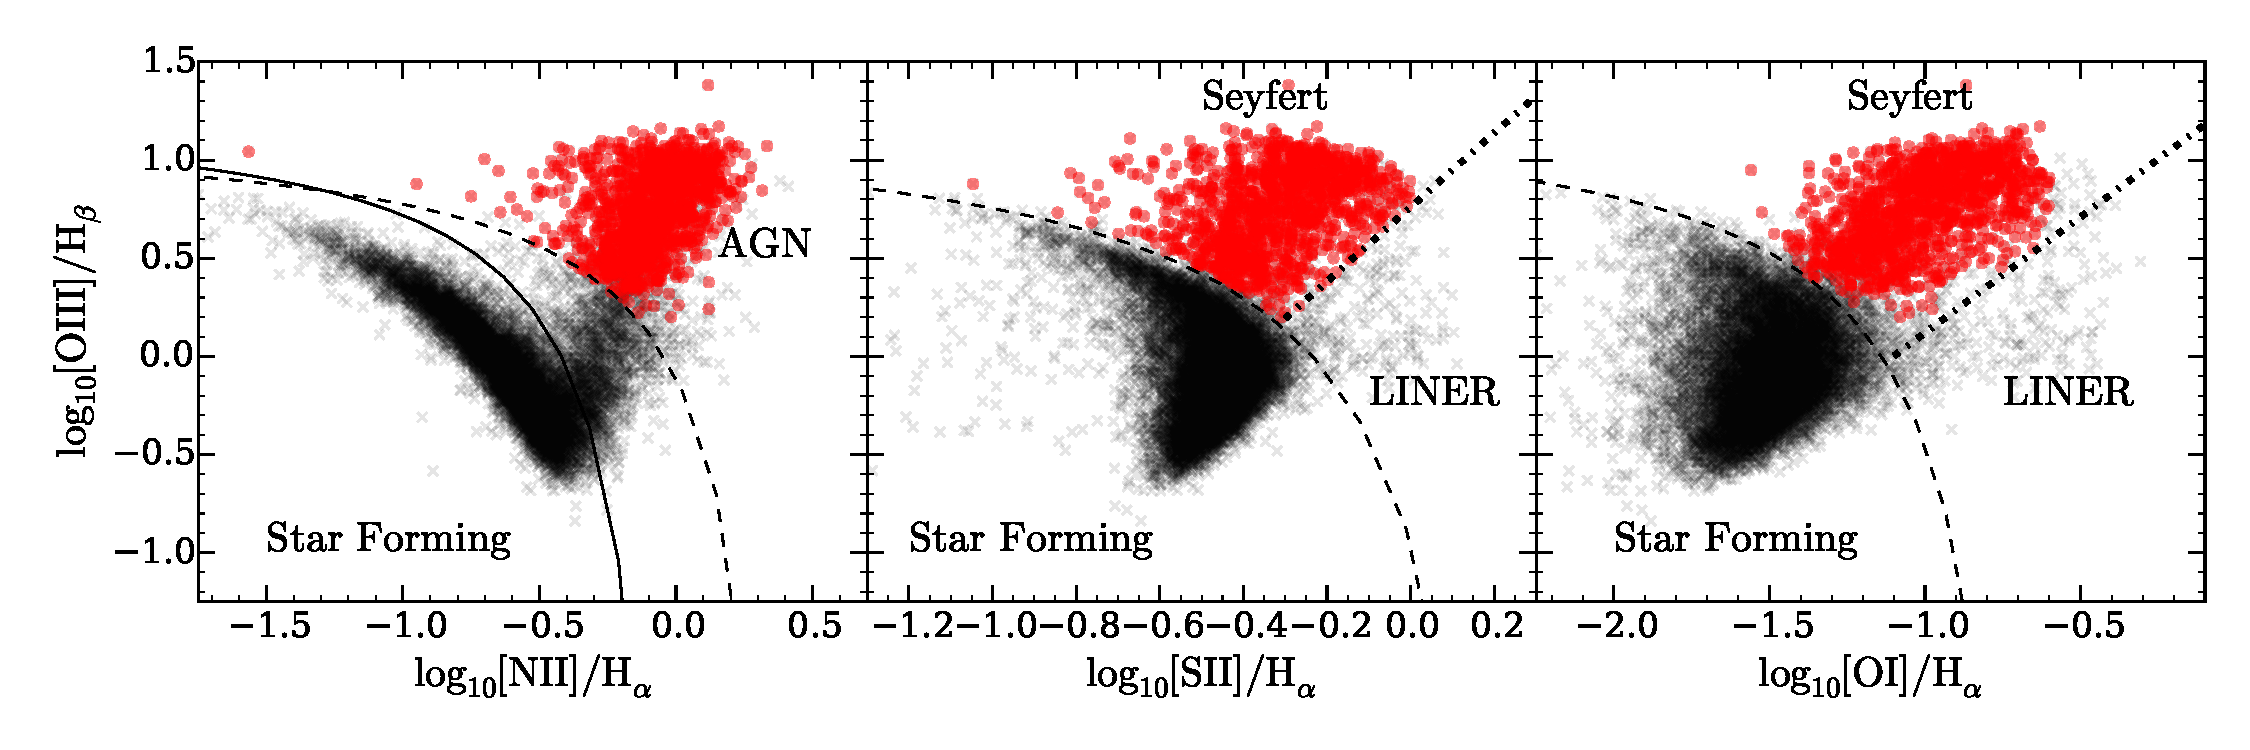
\includegraphics[width=\textwidth]{agn/fig2.pdf}
\caption[BPT diagram used to select AGN host galaxies]{BPT diagrams for galaxies in the \textsc{gz2-galex} sample (black crosses) with S/N $> 3$ for each emission line. Inequalities defined in: \protect\cite{kewley01} to separate SF galaxies from AGN (dashed lines), \protect\cite{kauffmann03b} to separate SF from composite SF-AGN galaxies (solid line) and \protect\cite{kewley06} to separate LINERS and Seyferts (dotted lines). Galaxies are included in the \textsc{agn-host} sample (red circles) if they satisfy all the inequalities to be classified as Seyferts. LINERs are excluded for purity.}
\label{bpt}
\end{figure*}

\begin{figure*}
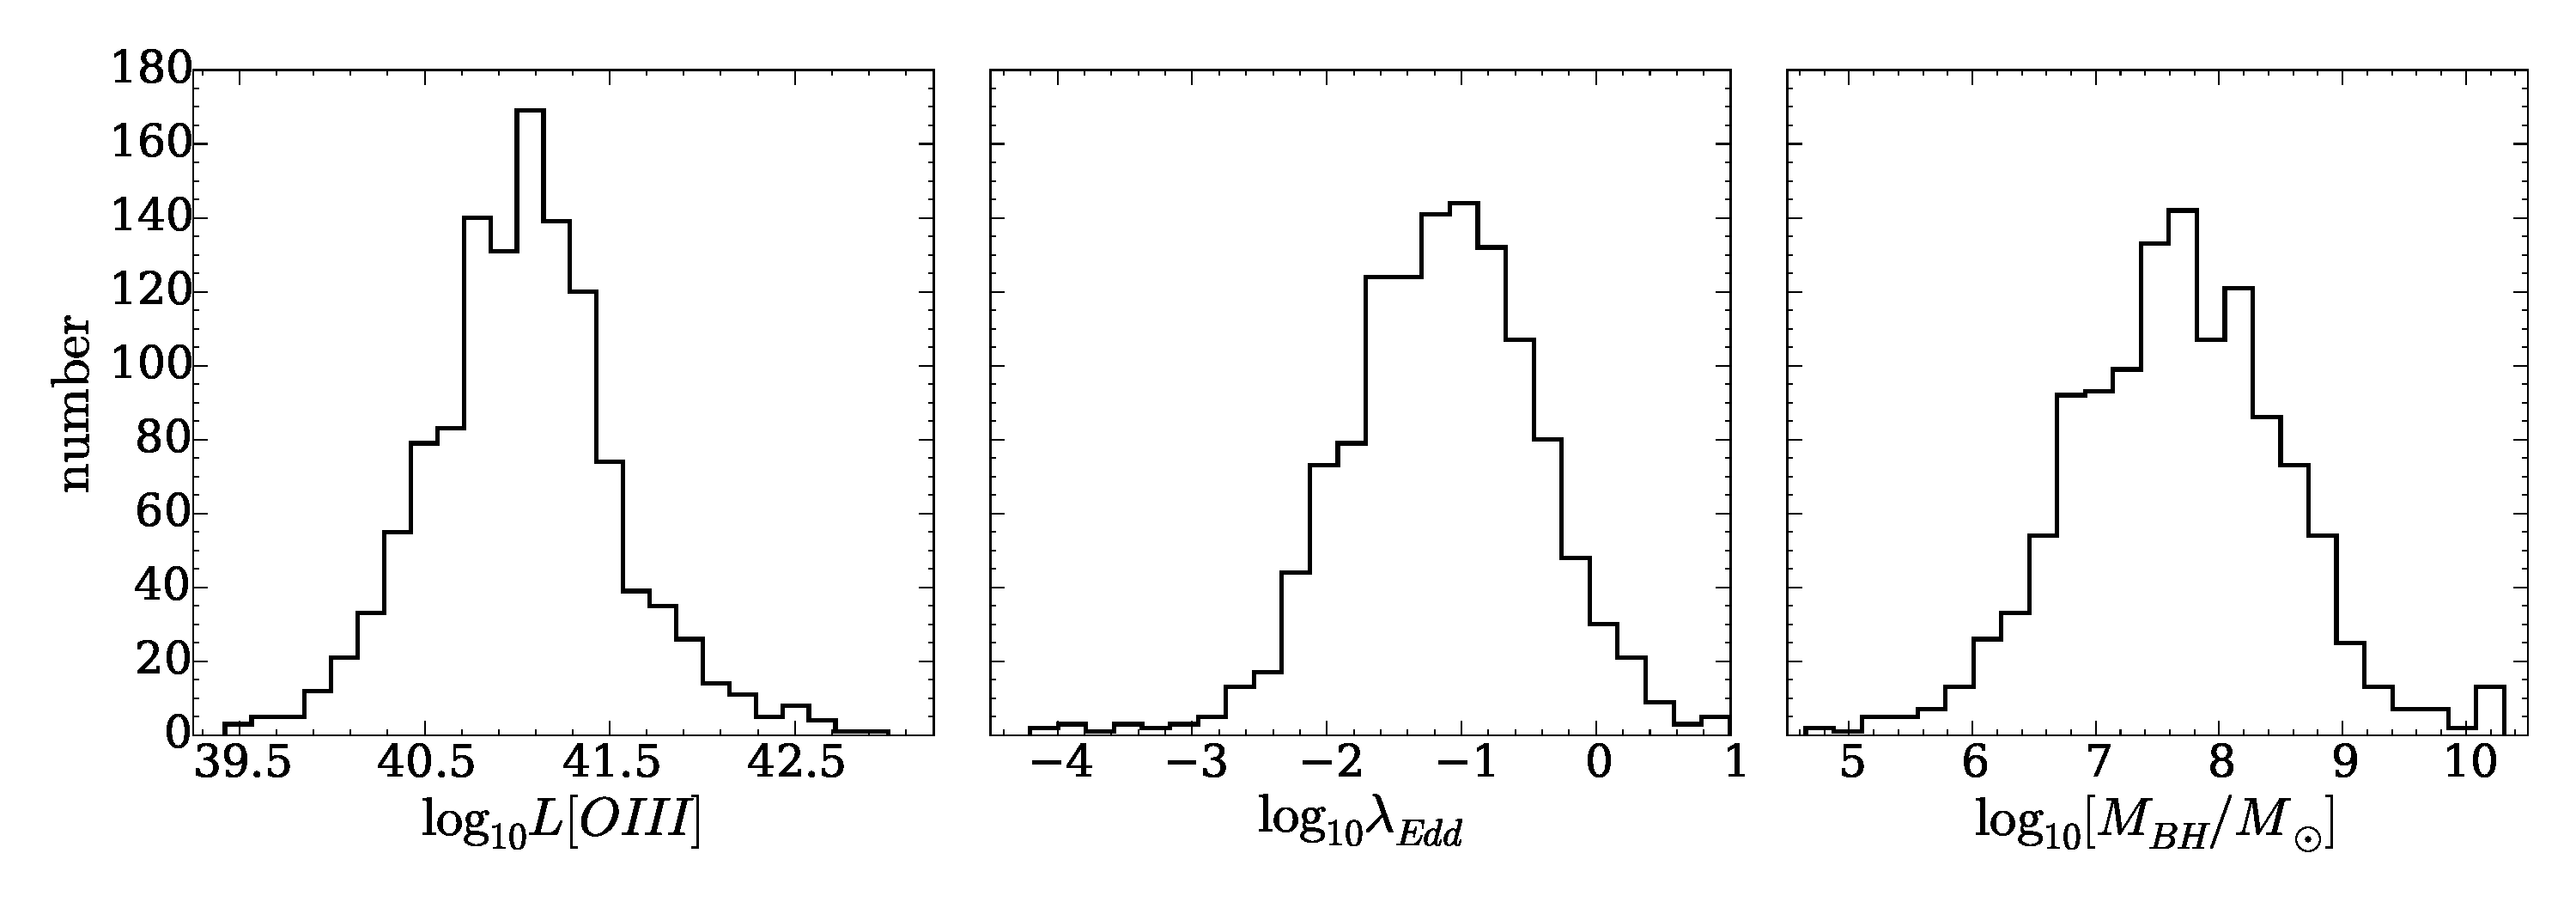
\includegraphics[width=\textwidth]{agn/agn-host_distributions_loiii_edd_ratio_mbh.pdf}
\caption[Distribution of measured galaxy parameters in the \textsc{agn-host} sample]{Distribution of the [OIII] luminosity (left), Eddington ratio (middle) and black hole masses (right) in the \textsc{agn-host} sample.}
\label{fig:agndistributions}
\end{figure*}


Type 2 AGN were selected from the \textsc{gz2-galex} sample using a BPT diagram \citep{bpt} using line and continuum strengths for [OIII], [NII], [SII] and [OII] obtained from the MPA-JHU catalogue \citep{kauffmann03, brinchmann04}. A BPT diagram uses emission line ratio diagnostics to determine whether a galaxy is a star forming galaxy, a Seyfert (i.e. hosting an AGN) or a LINER. The signal-to-noise ratio was required to be S/N $> 3$ for each emission line as in \cite{schawinski10a}. Those galaxies which satisfied all of the inequalities defined in \citet[][to separate SF galaxies from AGN]{kewley01} and \citet[][to separate SF galaxies from composite SF-AGN galaxies]{kauffmann03b} were selected as Type 2 AGN, giving $1,299$ host galaxies ($\sim10\%$ of the \textsc{gz2-galex} sample; in agreement with estimates of the local AGN fraction of \citealt{kauffmann04, pimbblet13}).

\cite{Sarzi10, yan12} and \cite{Singh13} have all demonstrated that LINERs are not primarily powered by AGN, therefore for purity, these galaxies were excluded from the sample using the definition from \cite[][$55$ galaxies total]{kewley06} with no change to the results. These $1,244$ galaxies will be referred to as the \textsc{agn-host} sample; Figure~\ref{bpt} shows the entire \textsc{agn-host} and \textsc{gz2-galex} samples with the selection criteria used on a BPT diagram.

I do not use Type 1 AGN in this instance due to concerns about contamination of the observed galaxy colours, used in the SFH analysis, from potentially strong NUV emission by unobscured active nuclei. The obscuration of Type 2 AGN is highly efficient, considerably more so in the NUV than the optical \citep{Simmons11}. Residual NUV flux from a Type 2 AGN can therefore be neglected in comparison to that of the galaxy. However, I did investigate the possibility of contamination of optical galaxy colours from unobscured AGN emission and found that subtracting measured nuclear magnitudes (SDSS {\tt psfMag}) from the total galaxy magnitude (SDSS {\tt modelMag}) produces a negligible change in host galaxy colour ($\Delta(u-r) \sim 0.09$). I therefore use the total galaxy magnitudes (with extinction corrections as described in Section~\ref{sec:sample}) to avoid unnecessary complexity and minimise the propagation of uncertainty from the observed colours through to the inferred SFHs. However, I note that including these corrected colours does not change the results.

\begin{figure*}
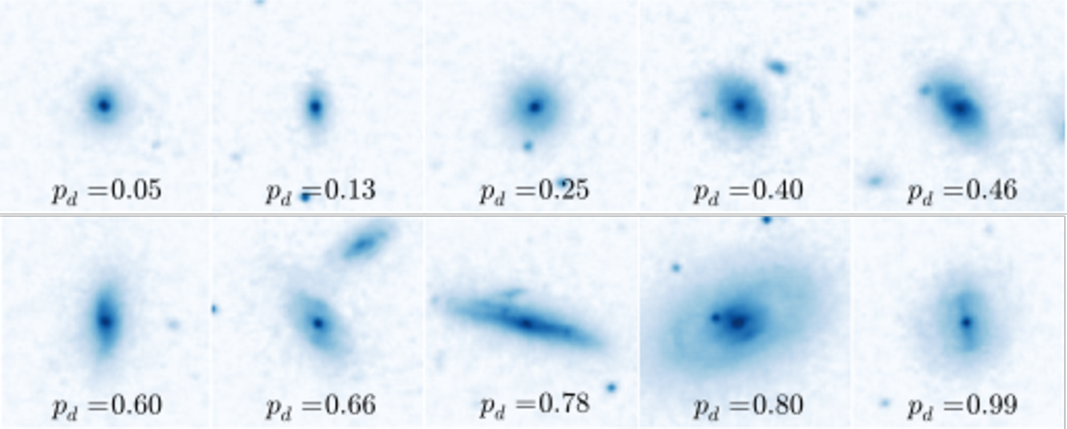
\includegraphics[width=\textwidth]{agn/fig1.pdf}
\caption[SDSS images of galaxies in the \textsc{agn-host} sample]{Randomly selected SDSS \emph{gri} composite images from the sample of $1,244$ Type 2 AGN in a redshift range $0.04 < z < 0.05$.  The galaxies are ordered from least to most featured according to their debiased `disc or featured' vote fraction, $p_d$ (see \citealt{GZ2}). The scale for each image is $0.099~\rm{arcsec/pixel}$.}
\label{mosaic}
\end{figure*}

Since this investigation is focussed on whether an AGN can have an impact on the SF of its host galaxy, possible selection effects must be considered. The extent to which SF could obscure AGN emission was addressed by \cite{schawinski10a}. They showed, via analysis of simulated AGN emission added to star-forming galaxies, that BPT-based selection of AGN produces a complete sample at luminosities of $L[OIII] > 10^{40}~\rm{erg~s}^{-1}$. Above this limit I therefore assume I have selected a complete sample of AGN independent of host galaxy SFR. 

Black hole masses of the \textsc{agn-host} sample are derived from the $M_{BH}-\sigma$ relationship defined in \citet{mcconnell11}:
\begin{equation}
\log_{10}\left(\frac{M_{BH}}{M_{\odot}}\right) = 8.29 + 5.12 ~\log_{10}\left(\frac{\sigma}{200 ~\rm{km} ~s^{-1}}\right). 
\end{equation}
where the velocity dispersion, $\sigma$, is measured from the Balmer lines and is provided in the MPA-JHU catalog \citep{kauffmann03, brinchmann04}. The Eddington ratio, $\lambda_{Edd}$, describes the accretion rate of the black hole and is calculated with the proxy $\lambda_{Edd} = L_{bol}/L_{Edd}$, where $L_{Edd}$ is the Eddington luminosity and $L_{bol}$ is the bolometric luminosity. For obscured (Type 2) AGN the bolometric luminosity cannot be directly measured and so is inferred from the luminosity of the [OIII] emission line, as derived by \citet{heckman04}:
\begin{equation}
\log_{10}L_{bol} = 3.54 + \log_{10}L[OIII]. 
\end{equation}
The Eddington luminosity, $L_{Edd}$, is derived from the black hole mass, $M_{BH}$, as outlined in \citet{binneymerrifield} as:
\begin{equation}
L_{Edd} = 3\times10^4 \left(\frac{M_{BH}}{M_{\odot}}\right) L_{\odot}.
\end{equation}
The distributions of L[OIII], $M_{BH}$ and $\lambda_{Edd}$ of the \textsc{agn-host} sample are shown in Figure~\ref{fig:agndistributions}. SDSS images for 10 randomly selected galaxies from the \textsc{agn-host} sample are shown in Figure~\ref{mosaic}. The decomposition of the \textsc{agn-host} sample into red sequence, green valley and blue cloud galaxies is shown in Tables~\ref{table:agnsubs} and \ref{table:agnqsubs} along with further division by galaxy type and SFR (where available for the \textsc{agn-host} sample from the MPA-JHU catalog) respectively. 


\begin{table}
\caption{Table showing the decomposition of the \textsc{agn-host} sample by galaxy type into the subsets of the colour-magnitude diagram.}
\begin{tabular*}{\textwidth}{l @{\extracolsep{\fill}}cccc}
\hline
\begin{tabular}[c]{@{}c@{}} {\color{white} -} \\ {\color{white} -}  \end{tabular} & All                                                      & Red Sequence                                              & Green Valley                                              & Blue Cloud \\  \hline 
Smooth-like ($p_s > 0.5$)        & \begin{tabular}[c]{@{}c@{}}340\\ (27.3\%)\end{tabular} & \begin{tabular}[c]{@{}c@{}}21\\ (25.0\%)\end{tabular}  & \begin{tabular}[c]{@{}c@{}}105\\ (41.2\%)\end{tabular}   & \begin{tabular}[c]{@{}c@{}}213\\ (23.5\%)\end{tabular}  \\ 
Disc-like ($p_d > 0.5$)          & \begin{tabular}[c]{@{}c@{}}871\\ (70.0\%)\end{tabular} & \begin{tabular}[c]{@{}c@{}}63\\ (75.0\%)\end{tabular}   & \begin{tabular}[c]{@{}c@{}}148\\ (58.0\%)\end{tabular}  & \begin{tabular}[c]{@{}c@{}}660\\ (72.9\%)\end{tabular}  \\
Early-type ($p_s \geq 0.8$) & \begin{tabular}[c]{@{}c@{}}66\\ (5.3\%)\end{tabular}  & \begin{tabular}[c]{@{}c@{}}1\\ (1.2\%)\end{tabular}    & \begin{tabular}[c]{@{}c@{}}14\\ (5.5\%)\end{tabular}    & \begin{tabular}[c]{@{}c@{}}51\\ (5.6\%)\end{tabular}    \\
Late-type ($p_s \geq 0.8$)  & \begin{tabular}[c]{@{}c@{}}569\\ (45.7\%)\end{tabular} & \begin{tabular}[c]{@{}c@{}}39\\ (46.4\%)\end{tabular}    & \begin{tabular}[c]{@{}c@{}}74\\ (29.0\%)\end{tabular}    & \begin{tabular}[c]{@{}c@{}}456\\ (50.4\%)\end{tabular}  \\ \hline
\textbf{Total}                       & \begin{tabular}[c]{@{}c@{}}\textbf{1244} \\ (100.0\%)\end{tabular}                                                & \begin{tabular}[c]{@{}c@{}}84 \\ (6.7\%)\end{tabular} & \begin{tabular}[c]{@{}c@{}}255 \\ (20.5\%)\end{tabular} & \begin{tabular}[c]{@{}c@{}}905 \\ (72.7\%)\end{tabular} \\\hline
\end{tabular*}
\label{table:agnsubs}
\end{table}


\begin{table}
\caption{Table showing the decomposition of the \textsc{agn-host} sample galaxies by their star formation rate in the subsets of the colour-magnitude diagram.}
\begin{tabular*}{\textwidth}{l @{\extracolsep{\fill}}cccc}
\hline
\begin{tabular}[c]{@{}c@{}} {\color{white} -} \\ {\color{white} -}  \end{tabular} 		& All                                                      						& Red Sequence                                              			& Green Valley                                             			 & Blue Cloud \\  \hline 
\begin{tabular}[l]{@{}l@{}}Quenched\\ ($\rm{SFR} < P - 5\sigma$) \end{tabular}				& \begin{tabular}[c]{@{}c@{}}14\\ (1.3\%)\end{tabular} 			& \begin{tabular}[c]{@{}c@{}}9\\ (12.5\%)\end{tabular}    & \begin{tabular}[c]{@{}c@{}}4\\ (1.7\%)\end{tabular}    & \begin{tabular}[c]{@{}c@{}}1\\ (0.1\%)\end{tabular}  \\ 
\begin{tabular}[l]{@{}l@{}}Quenching\\ ($P - 5\sigma < \rm{SFR} < P - \sigma$) \end{tabular}	 & \begin{tabular}[c]{@{}c@{}}335\\ (30.6\%)\end{tabular}			 & \begin{tabular}[c]{@{}c@{}}45\\ (64.3\%)\end{tabular}    & \begin{tabular}[c]{@{}c@{}}139\\ (59.9\%)\end{tabular}    & \begin{tabular}[c]{@{}c@{}}151\\ (19.1\%)\end{tabular}  \\ 
\begin{tabular}[l]{@{}l@{}}Star Forming  \\ ($\rm{SFR} > P -\sigma$) \end{tabular} 			& \begin{tabular}[c]{@{}c@{}}744\\ (68.0\%)\end{tabular} 			& \begin{tabular}[c]{@{}c@{}}16 \\ (22.9\%)\end{tabular}    & \begin{tabular}[c]{@{}c@{}}89\\ (38.4\%)\end{tabular}    & \begin{tabular}[c]{@{}c@{}}639\\ (80.7\%)\end{tabular}  \\ \hline
\textbf{Total}                       														& \begin{tabular}[c]{@{}c@{}}\textbf{1093} \\ (100.0\%)\end{tabular} & \begin{tabular}[c]{@{}c@{}}70 \\ (6.4\%)\end{tabular} & \begin{tabular}[c]{@{}c@{}}232 \\ (21.2\%)\end{tabular} & \begin{tabular}[c]{@{}c@{}}791 \\ (72.4\%)\end{tabular} \\\hline
\end{tabular*}
\label{table:agnqsubs}
\end{table}


\subsection{Defining a control sample}

\begin{figure*}
\centering
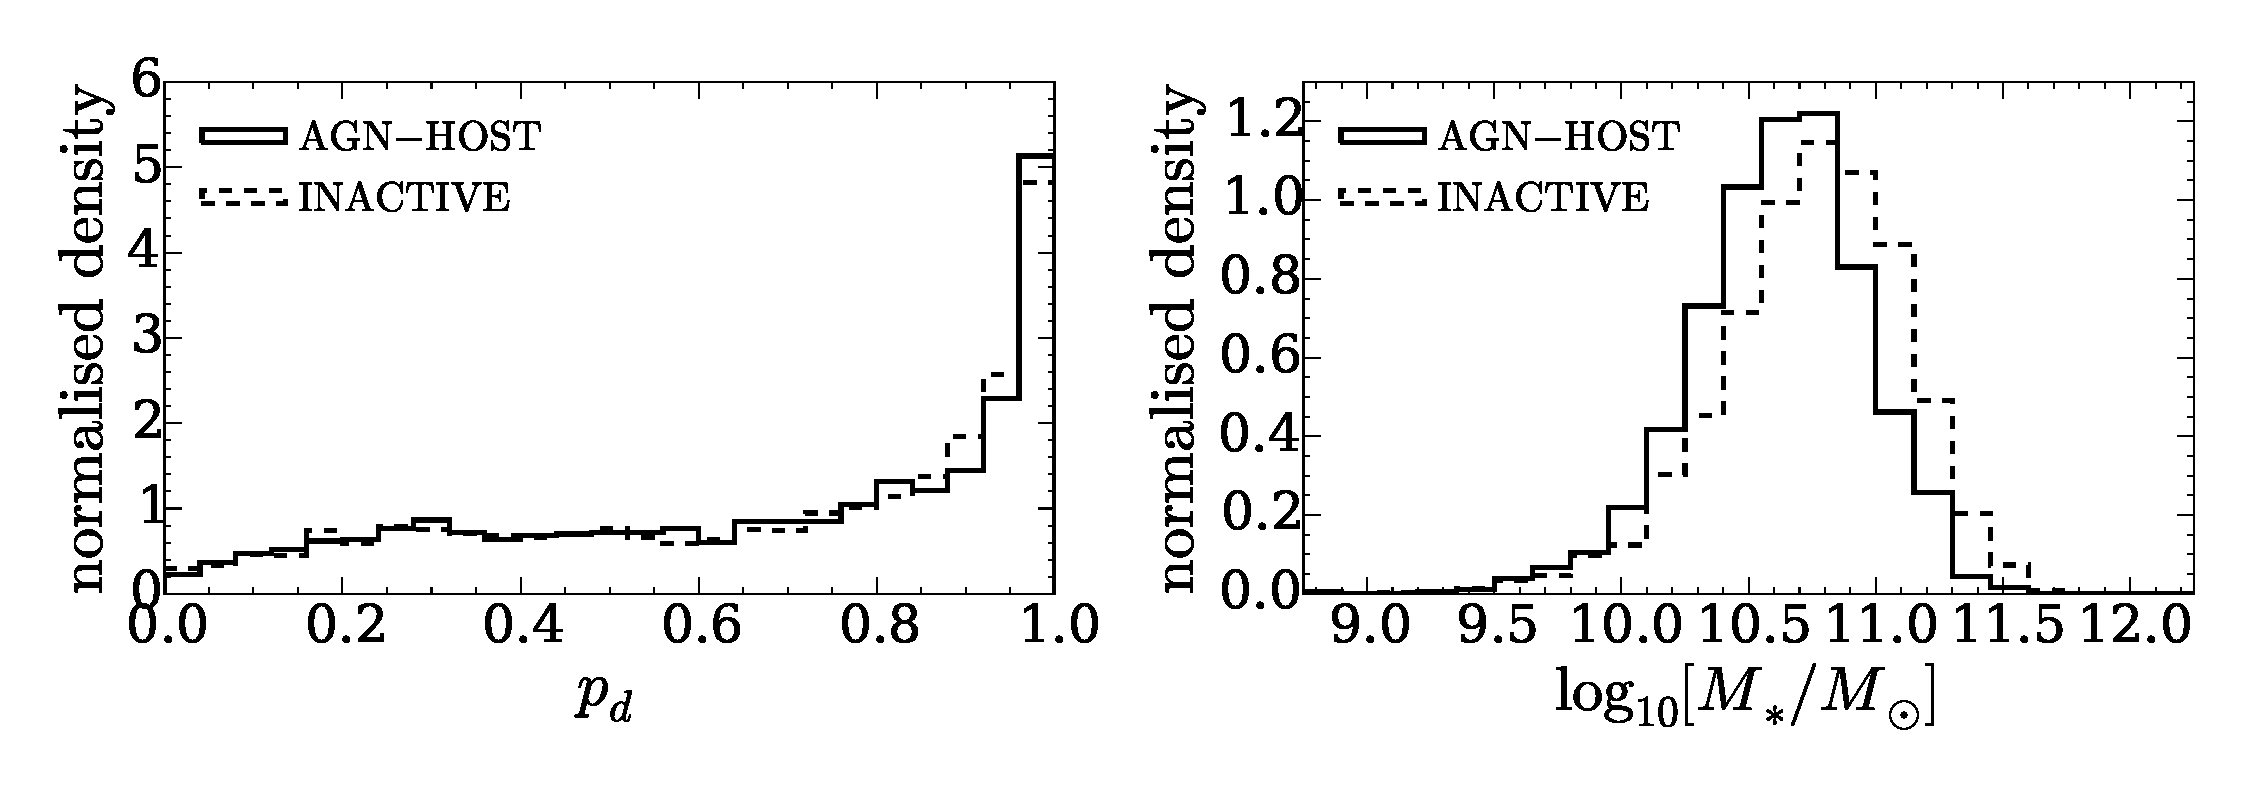
\includegraphics[width=\textwidth]{agn/agn-host_inactive_pd_mass_distributions.pdf}
\caption[Morphology and mass distributions of the \textsc{agn-host} and \textsc{inactive} samples]{Distribution of the GZ2 disc vote fractions ($p_d$; left) and stellar masses (right) in the \textsc{agn-host} sample (solid lines) in comparison to the matched control \textsc{inactive} sample (dashed lines).}
\label{fig:zmdistmatch}
\end{figure*}

\begin{figure}
\centering
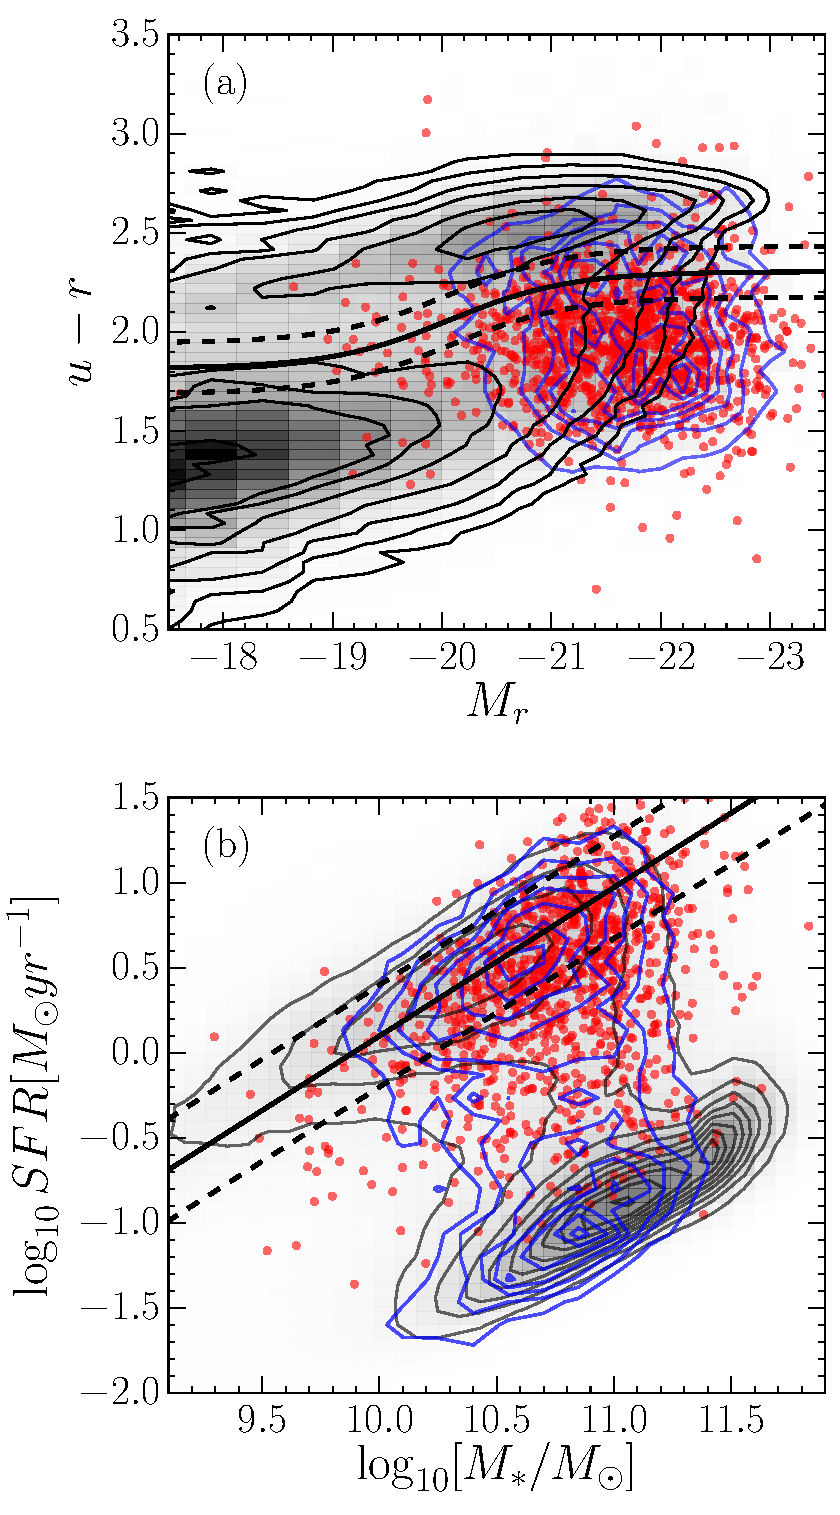
\includegraphics[height=0.75\textheight]{agn/fig3.pdf}
\caption[Colour-magnitude and SFR-mass diagram for \textsc{agn-host} galaxies]{(a) Optical colour-magnitude diagram showing the SDSS DR7 (grey filled contours), the \textsc{agn-host} sample (red circles) and \textsc{inactive} sample (blue contours). The definition of the green valley from \citet{Baldry06} (solid line) with $\pm 1\sigma$ (dashed lines) is shown. (b) SFR-stellar mass diagram showing the MPA-JHU measurements of SFR and $M_*$ of SDSS DR7 galaxies (\citealt{kauffmann03, brinchmann04}; black contours), the \textsc{agn-host} sample (red circles) and \textsc{inactive} sample (blue contours). The star forming `main sequence' from \citet{peng10} is shown by the solid line for $t = 12.8~\rm{Gyr}$, the average observed age of the \textsc{gz2-galex} sample, with $\pm1\sigma$ (dashed lines).}
\label{cmdsfms}
\end{figure}


A control sample of inactive galaxies was constructed by removing from the \textsc{gz2-galex} sample all galaxies with line strengths indicative of potential AGN activity \citep{kauffmann03b}, as well as sources identified as Type 1 AGN by the presence of broad emission lines \citep{Oh15}.  I selected a mass- and morphology-matched inactive sample by identifying between 1 and 5 inactive galaxies for each \textsc{agn-host} galaxy with the same stellar mass (to within $\pm5\%$) and GZ2 `smooth' and `disc' vote fractions (to within $\pm 0.1$) giving $6107$ galaxies. This sample will be referred to as the \textsc{inactive} sample. 


Figure~\ref{fig:zmdistmatch} shows the GZ2 disc vote fraction ($p_d$; left) and stellar mass ($M_*$; right) distributions of the \textsc{agn-host} sample in comparison to the matched \textsc{inactive} sample. A Kolmogorov-Smirnov test revealed the redshift distributions of the \textsc{inactive} and \textsc{agn-host} samples are statistically indistinguishable ($D \sim 0.16$, $p \sim 0.88$). 

The \textsc{agn-host} and \textsc{inactive}  samples are also shown on both an optical colour-magnitude diagram and in the SFR-stellar mass plane in Figure~\ref{cmdsfms} in comparison to the distribution of SDSS DR7 galaxies. SFRs and stellar masses are obtained from the MPA JHU catalog, where available, which follow the prescriptions outlined in \cite{brinchmann04} and \cite{Salim07} for calculating the total aperture corrected galaxy SFR in the presence of an AGN. 

The majority of the \textsc{agn-host} sample would be defined as residing in the blue cloud ($\sim73\%$) on the optical colour-magnitude diagram despite the fact that a significant proportion of the sample ($32\%$) lie more than $1\sigma$ ($0.3$ $\rm{dex}$) below the star forming `main sequence' \citep[][see Figure \ref{cmdsfms} and Table~\ref{table:agnqsubs}]{peng10}.

\subsection{Results}\label{results}

\begin{figure}
\centering{
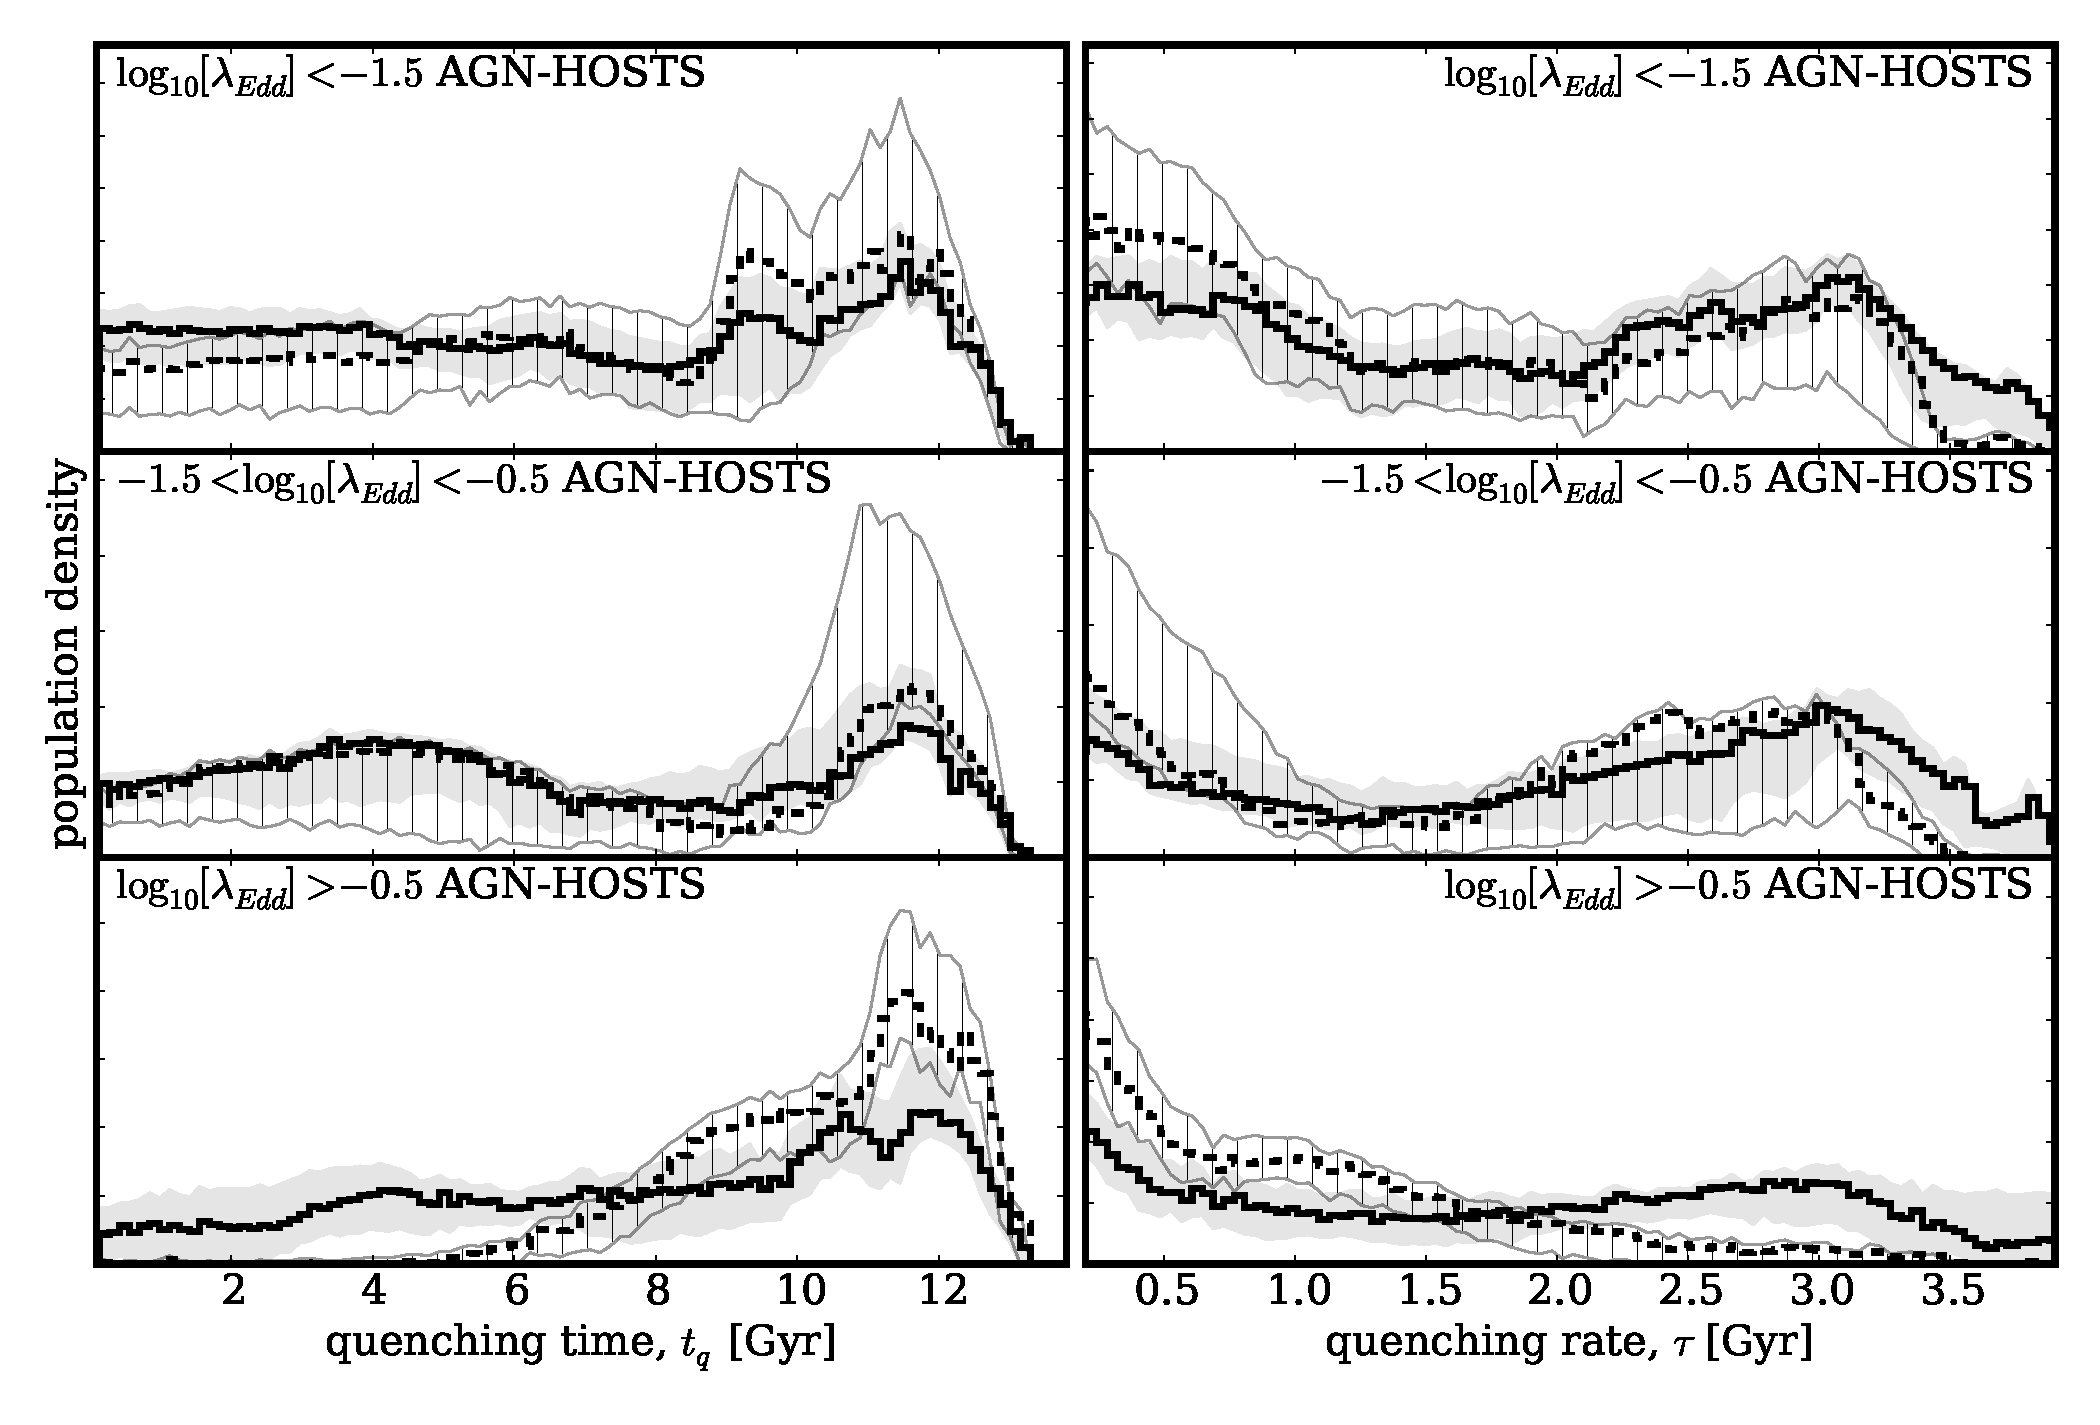
\includegraphics[width=0.92\textwidth]{agn/fig6.pdf}}
\caption[Quenching time and rate population density distributions for the \textsc{agn-host} sample split by Eddington ratio]{Population density distributions for the quenching time ($t_q$; left) and rate ($\tau$; right), normalised so that the areas under the curves are equal. The \textsc{agn-host} sample is split into low (top), medium (middle) and high (bottom) Eddington ratio, $\lambda_{Edd}$, for smooth (dashed) and disc (solid) galaxies. Uncertainties from bootstrapping are shown by the shaded regions for the smooth (grey striped) and disc (grey solid) population densities. A small (large) value of $\tau$ corresponds to a rapid (slow) quench.}
\label{eddratiosplit}
\end{figure}

\begin{figure*}
\centering{
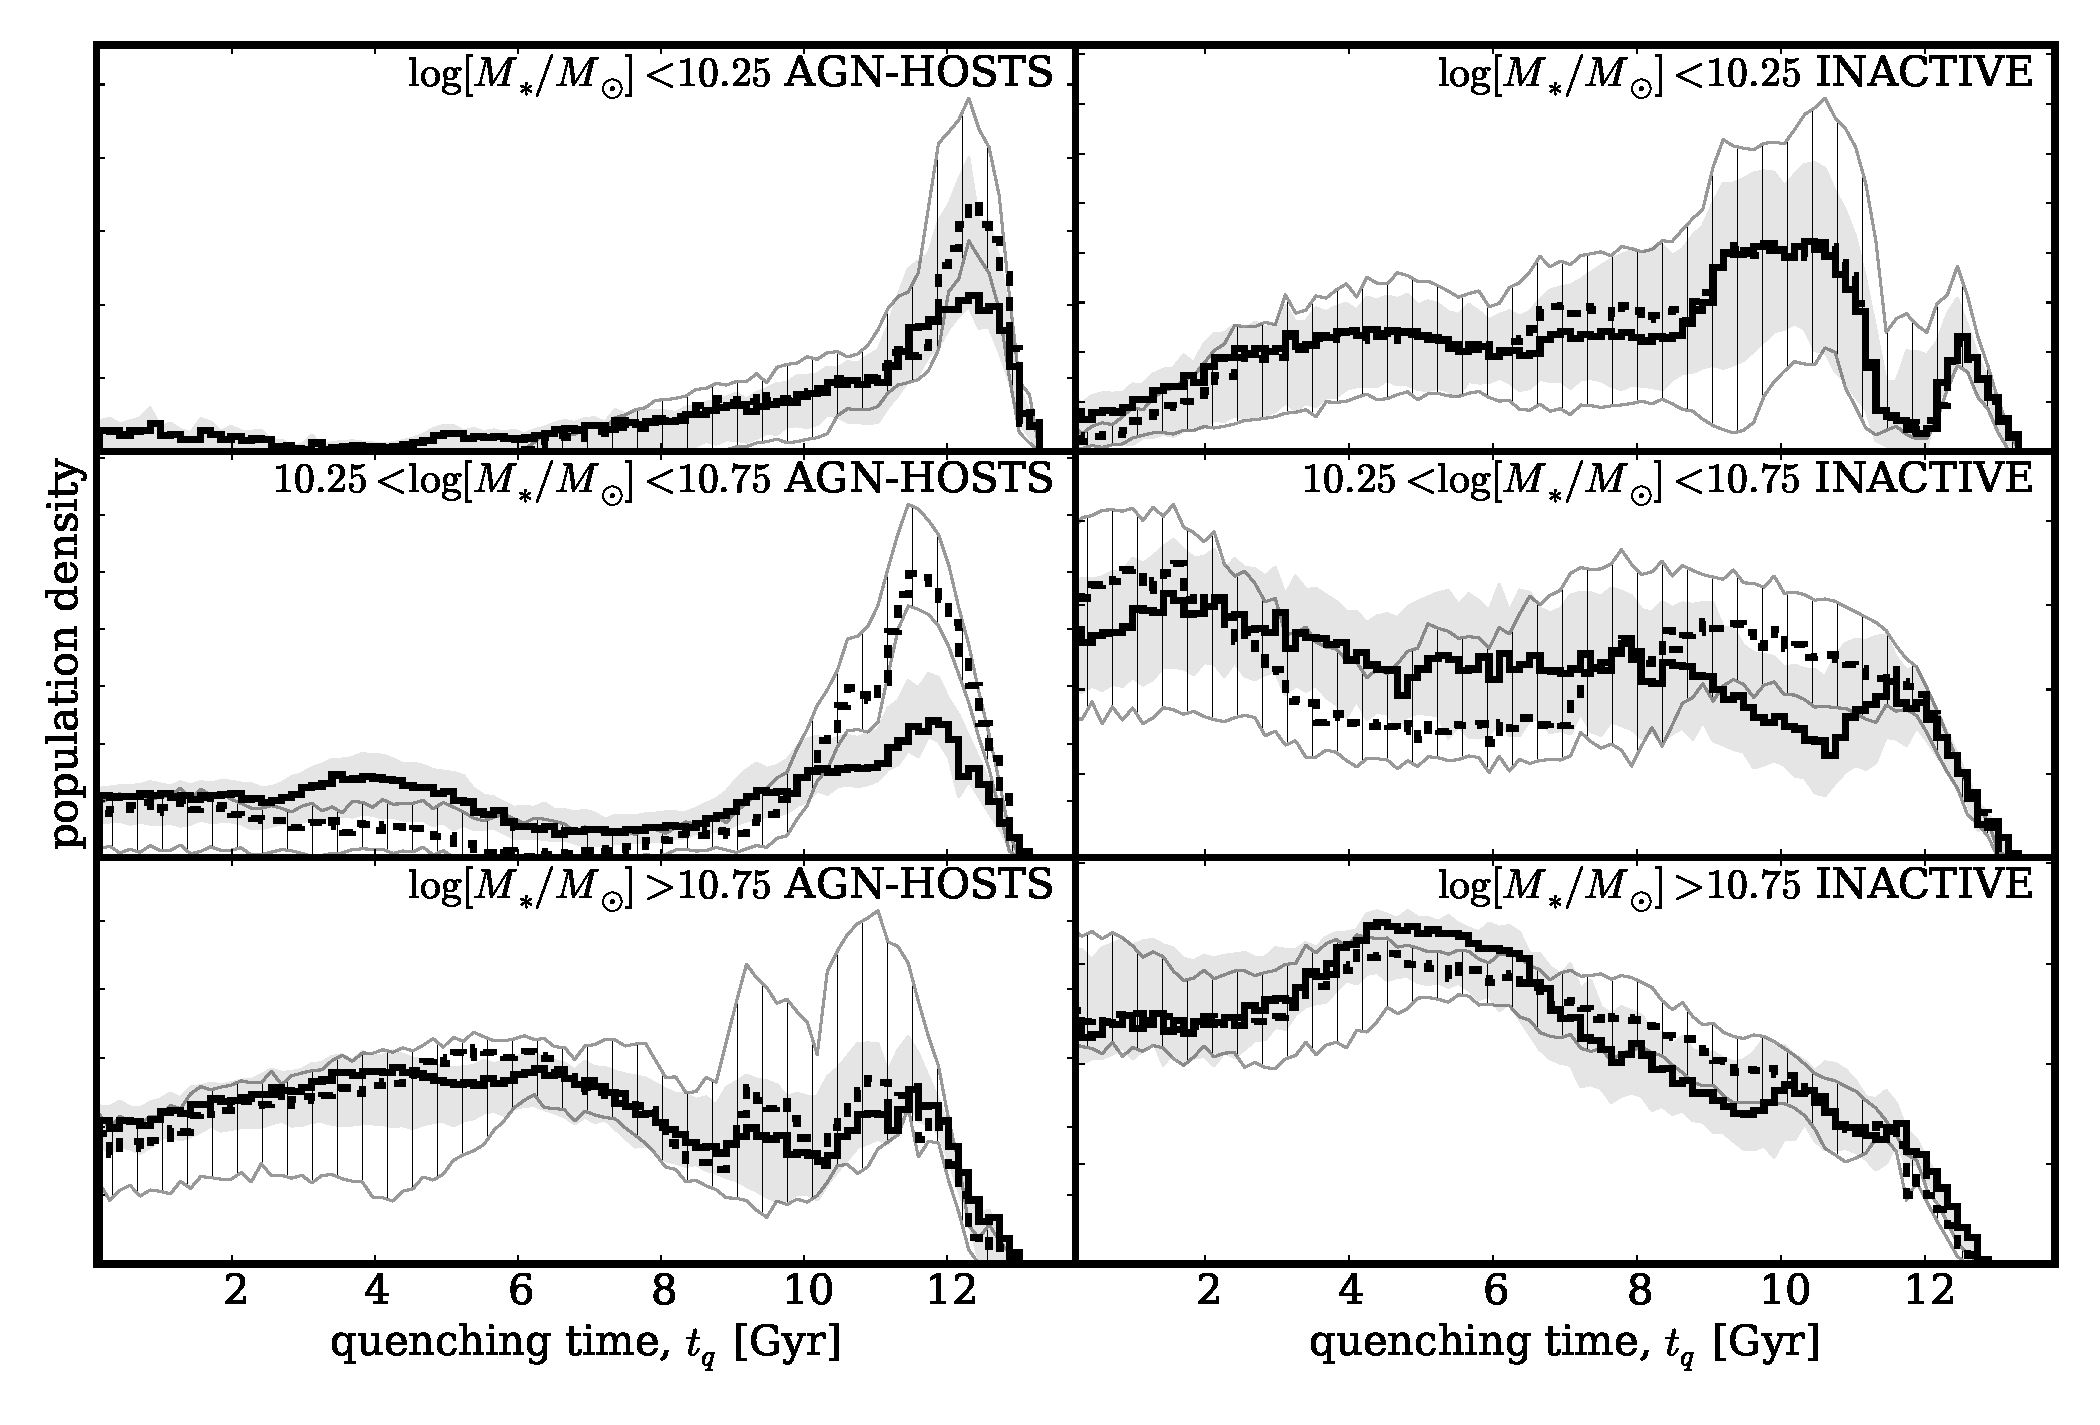
\includegraphics[width=0.92\textwidth]{agn/fig4.pdf}}
\caption[Quenching time population density distributions for the \textsc{agn-host} and \textsc{inactive} samples] {Population density distributions for the quenching time ($t_q$) parameter, normalised so that the areas under the curves are equal. \textsc{agn-host} (left) and \textsc{inactive} (right) galaxies are split into low (top), medium (middle) and high (bottom) mass for smooth (dashed) and disc (solid) galaxies. Uncertainties from bootstrapping are shown by the shaded regions for the smooth (grey striped) and disc (grey solid) population densities. A low (high) value of $t_q$ corresponds to the early (recent) Universe.}
\label{time}
\end{figure*}


\begin{figure*}
\centering{
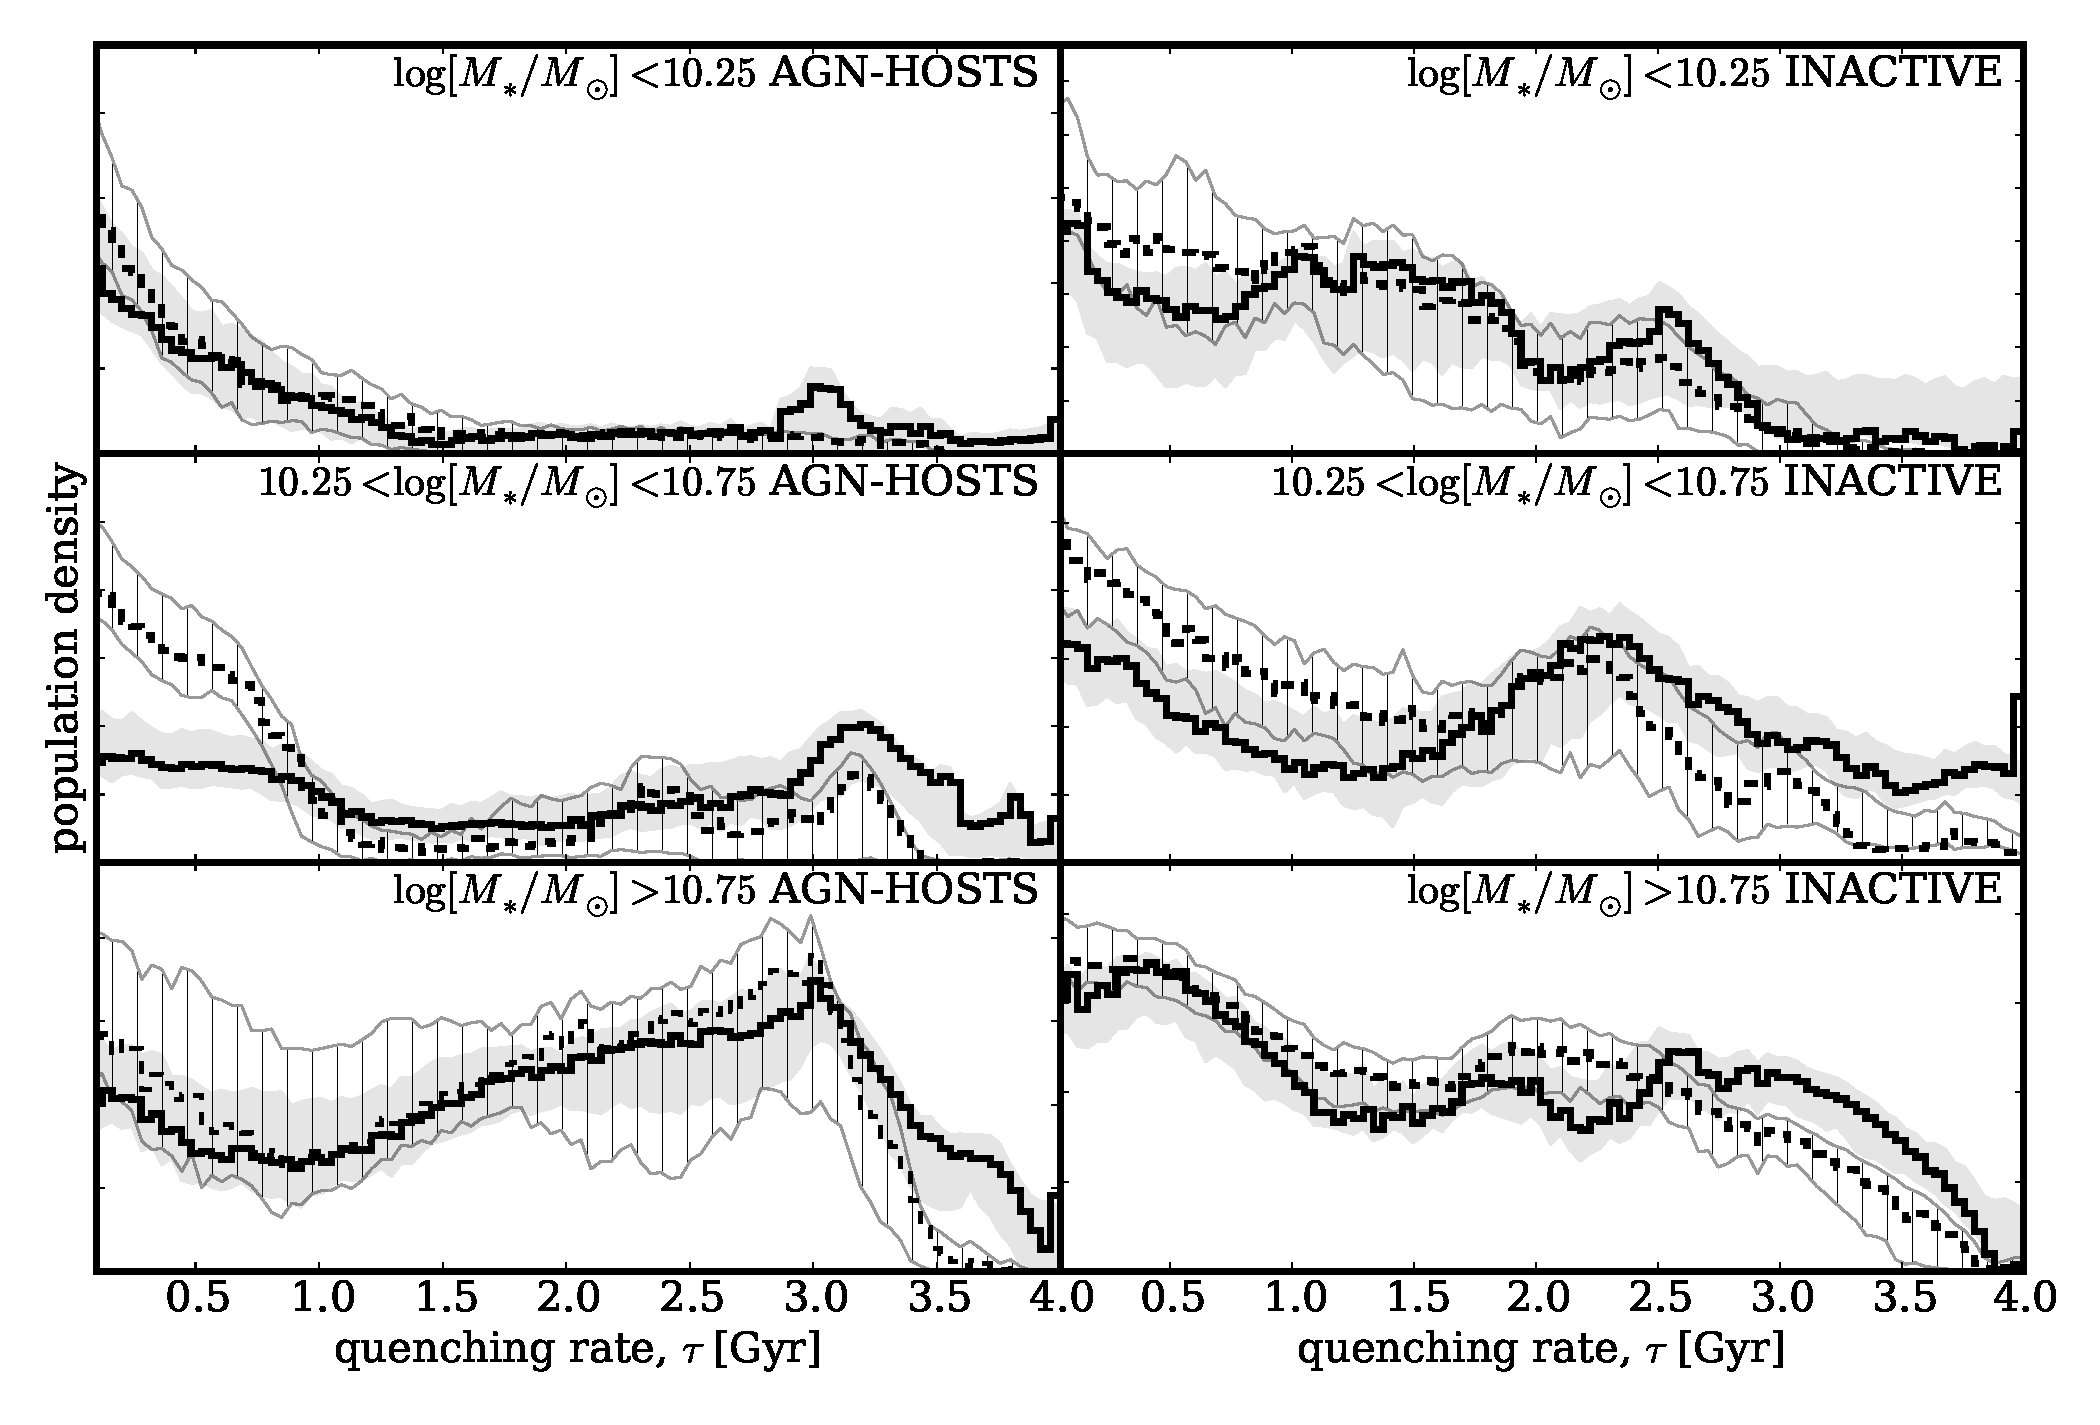
\includegraphics[width=0.92\textwidth]{agn/fig5.pdf}}
\caption[Quenching rate population density distributions for the \textsc{agn-host} and \textsc{inactive} samples]{Population density distributions for the quenching rate ($\tau$), normalised so that the areas under the curves are equal. \textsc{agn-host} (left) host and \textsc{inactive} (right) galaxies are split into low (top), medium (middle) and high (bottom) mass for smooth (dashed) and disc (solid) galaxies. Uncertainties from bootstrapping are shown by the shaded regions for the smooth (grey striped) and disc (grey solid) population densities. A small (large) value of $\tau$ corresponds to a rapid (slow) quench.}
\label{rate}
\end{figure*}


%Figures~\ref{eddratiosplit}, \ref{time} \& \ref{rate} show the population density distributions for the quenching time, $t_q$ and exponential quenching rate, $\tau$, with shaded regions to show the uncertainties for both smooth and disc weighted populations. 

In Figure \ref{eddratiosplit} the \textsc{agn-host} smooth and disc weighted populations are split across three Eddington ratio, $\lambda_{Edd}$, bins to investigate any trends with the accretion rate of the black hole in the population densities for the quenching time and rate. The Eddington ratio boundaries were chosen to give equal numbers of \textsc{agn-host} galaxies in each bin. 

In Figures~\ref{time} \& \ref{rate} the \textsc{agn-host} and \textsc{inactive} smooth and disc weighted populations are split across three mass bins to investigate any trends with mass in the population densities for the quenching time and rate respectively. The mass boundaries were chosen to give roughly equal numbers of inactive galaxies in each bin, before mass matching to the \textsc{agn-host} sample. This decision was made to ensure the mass bins were representative of `typical' galaxies rather than being biased by the mass distribution of the \text{agn-host} sample which tend to occupy higher mass galaxies. 

No cut on the star formation rate is made to the galaxies which contribute to Figures \ref{eddratiosplit}-\ref{rate}, but those galaxies poorly fit by an exponentially declining SFH are down-weighted so that they do not contribute to the results presented here (see Section~\ref{popstarpy} for a description of the \textsc{popstarpy} method). Table~\ref{massbins} contains the percentages of the population densities shown in Figures~\ref{time} \& \ref{rate} in the quenching regimes originally defined in Chapter~\ref{morph} for rapid ($\tau < 1$ Gyr), intermediate ($1 < \tau ~\rm{[Gyr]} < 2$) and slow ($\tau > 2$ Gyr) quenching rates in each of the three mass bins. Uncertainties on the population densities (shown by the shaded regions) are determined from the maximum and minimum values spanned by $N = 1000$ bootstrap iterations, each sampling $90\%$ of the galaxy population. $1\sigma$ uncertainties are quoted for the percentages in Table~\ref{massbins}, calculated from the bootstrapped distributions.


\begin{table*}
{\tiny
\centering{
\caption{Table showing the number of galaxies in each of the three mass bins for both the \textsc{agn-hosts} and \textsc{inactive} galaxy samples and the percentage of the distribution across each morphologically weighted population found in the rapid, intermediate and slow quenching regimes.}
\label{massbins}
\begin{tabular}{c|c|c|c|c|c|c}
\hline
\textsc{sample}                     & \textsc{mass bin}                                        & \textsc{weighting}                  & $\tau < 1 ~\rm{[Gyr]}$                             & $1 < \tau ~\rm{[Gyr]} < 2 $          & $\tau > 2 ~\rm{[Gyr]}$                               & \textsc{number}                                        \\ \hline \hline
\multirow{6}{*}{AGN-HOSTS} & \multirow{2}{*}{$\log [M_*/M_{\odot}] < 10.25 $}                       & $p_d$     & $60\pm_{5}^{23}$                    & $13\pm_{9}^{9}$                    & $28\pm_{19}^{6}$       & \multirow{2}{*}{$165 (13.3\%)$}                      \\
                           &                                                 & $p_s$     & $69\pm_{6}^{14}$                    & $17\pm_{14}^{6}$                   & $14\pm_{7}^{3}$        &                                                      \\ \cline{2-7} 
                           & \multirow{2}{*}{$10.25 < \log [M_*/M_{\odot}] < 10.75$}                    & $p_d$     & $33\pm_{5}^{3}$                     & $15\pm_{4}^{4}$                    & $51\pm_{7}^{4}$        & \multirow{2}{*}{$630 (50.6\%)$}                      \\
                           &                                                 & $p_s$     & $69\pm_{5}^{4}$                     & $7\pm_{4}^{4}$                     & $26\pm_{9}^{5}$        &                                                      \\ \cline{2-7} 
                           & \multirow{2}{*}{$\log [M_*/M_{\odot}] > 10.75$}                      & $p_d$     & $20\pm_{4}^{5}$ & $25\pm_{5}^{7}$                    & $56\pm_{12}^{8}$       & \multirow{2}{*}{$449 (36.1\%)$}                      \\
                           &                                                 & $p_s$     & $24\pm_{3}^{4}$                     & $26\pm_{6}^{5}$                    & $50\pm_{7}^{7}$        &                                                      \\ \hline \hline
\multirow{6}{*}{INACTIVE}  & \multirow{2}{*}{$\log [M_*/M_{\odot}] < 10.25 $}                       & $p_d$     & $37\pm_{14}^{8}$                    & $39\pm_{6}^{8}$                    & $24\pm_{6}^{8}$        & \multirow{2}{*}{$807 (13.2\%)$}                      \\
                           &                                                 & $p_s$     & $47\pm_{11}^{5}$                    & $36\pm_{5}^{9}$                    & $17\pm_{5}^{4}$        &                                                      \\ \cline{2-7} 
                           & \multirow{2}{*}{$10.25 < \log [M_*/M_{\odot}] < 10.75$}                    & $p_d$     &          $30\pm_{3}^{4}$                          &       $18\pm_{3}^{2}$                            &    $51\pm_{4}^{4}$                   & \multirow{2}{*}{$3094 (50.7\%)$}                     \\
                           &                                                 & $p_s$     & $42\pm_{2}^{2}$            & $29\pm_{3}^{3}$   & $30\pm_{4}^{3}$ &                                                      \\ \cline{2-7} 
                           & {\multirow{2}{*}{$\log [M_*/M_{\odot}] > 10.75$}} & $p_d$     & $36\pm_{3}^{3}$            & $24\pm_{4}^{3}$         & $41\pm_{3}^{4}$ & \multicolumn{1}{l}{\multirow{2}{*}{$2206 (36.1\%)$}} \\
                           & \multicolumn{1}{l|}{}                           & $p_s$      & $38\pm_{2}^{2}$              & $28\pm_{4}^{3}$            & $34\pm_{3}^{3}$ & \multicolumn{1}{l}{}                                 \\ \hline                       
\end{tabular}}}
\end{table*}

At all masses, the population density for galaxies within the \textsc{agn-host} population across the quenching time, $t_q$ (left panels of Figure~\ref{time}), is different from that of the inactive galaxies (right panels of Figure~\ref{time}). Recent quenching ($t > 11$ Gyr) is the dominant history for low and medium mass \textsc{agn-host} galaxies, particularly for the smooth weighted population hosting an AGN (solid lines, left panels Figure~\ref{time}). However, this effect is less dominant in higher mass galaxies where quenching at earlier times also has high density (bottom left panel of Figure \ref{time}).


The population densities for the quenching rate, $\tau$, in Figure~\ref{rate} and Table~\ref{massbins} show the dominance of rapid quenching ($\tau < 1$ Gyr) within the \textsc{agn-host} population, particularly for smooth galaxies (solid lines, left panels Figure~\ref{rate}). With increasing mass the dominant quenching rate becomes slow ($\tau > 2$ Gyr). Similar trends in the population density are observed for the \textsc{inactive} population (right panels Figure~\ref{rate}) but the overall distribution is very different. 

In Figure~\ref{eddratiosplit} there is no \textsc{inactive} control sample to act as a comparison, since an Eddington ratio cannot be measured for a black hole that is not accreting. The population densities for the \textsc{agn-host} samples however, show the dominance of rapid and recent quenching as the Eddington ratio increases (i.e. higher black hole accretion rates). A bimodal distribution can be seen for the low Eddington ratio \textsc{agn-host} population (top right panel of Figure~\ref{eddratiosplit}) between both rapid and slow quenching rates. 

The population densities for the \textsc{agn-host} galaxies therefore all show evidence for the dominance of rapid, recent quenching. This result implies the importance of AGN feedback for the evolution within this population.

\subsection{Discussion}\label{dis}

The differences between the population density distributions of the \textsc{agn-host} and \textsc{inactive} populations in Figures~\ref{time} \& \ref{rate} reveal that an AGN can have a significant effect on the SFH of its host galaxy. Both recent, rapid quenching and early, slow quenching are observed in the population densities of the \textsc{agn-host} population. 

There are however minimal differences between the smooth and disc weighted distributions of the quenching parameters within the \textsc{agn-host} population (comparing solid and dashed lines in the left panels of Figures~\ref{eddratiosplit} - \ref{rate}). This is agreement with the conclusions of \citet{kauffmann03b} who found that the structural properties of AGN hosts depend very little on AGN power. Quenching caused by AGN feedback is therefore morphologically independent; this is unlike the mechanisms discussed in Chapter~\ref{morph}.

Quenching at early times is observed within the \textsc{inactive} population (see right panels of Figure~\ref{time}), where the population density is roughly constant until recent times where the distribution drops off.  This drop-off occurs at earlier times with increasing mass, with a significant lack of quenching occurring at early times for low mass \textsc{inactive} galaxies (top right panel Figure~\ref{time}). This is evidence of downsizing within the \textsc{inactive} galaxy population whereby stars in massive galaxies form first and quench early \citep{Cowie96, Thomas10}. 

The population densities for smooth weighted higher mass (bottom left panels Figures~\ref{time} \& \ref{rate}) and lower Eddington ratio (top panels Figure \ref{eddratiosplit}) \textsc{agn-host} galaxies are also dominated by slow, early quenching. This implies that AGN feedback is not responsible for the cessation of star formation within a proportion of these galaxies, as this quenching has occurred prior to the triggering of the current AGN. I speculate that this is also due to the effects of downsizing rather than being caused by the current AGN. Since the lower Eddington ratio \textsc{agn-host} population is also dominated by this early quenching at slow rates (top panels Figure~\ref{eddratiosplit}) this supports the idea that the AGN is not strong enough to be the cause of this quenching.  This earlier evolution would first form a slowly `dying' or `dead' galaxy typical of massive elliptical galaxies which could then have a recent infall of gas either through a minor merger, galaxy interaction or environmental change, triggering further star formation and feeding the central black hole, triggering an AGN \citep{kaviraj14b}. In turn this AGN can then quench the recent boost in star formation. This track is similar to the evolution history proposed for blue ellipticals \citep[][and detected in the top panel of Figure~\ref{blue_c}]{Kaviraj13, McIntosh14, Haines15}. This SFH would then give rise to the distribution seen within the high mass smooth weighted \textsc{agn-host} population for both time and rate parameters (bottom panels of Figures~\ref{time} \& \ref{rate}).

Alternatively in the high mass disc weighted \textsc{agn-host} population, in which slow, early quenching is also observed (dashed lines bottom left panels of Figures~\ref{time} \& \ref{rate}) this evolution could be due to initially isolated discs evolving slowly by the Kennicutt-Schmidt \citep{Schmidt59, Kennicutt97} law which can then undergo an interaction or merger to reinvigorate star formation, feed the central black hole and trigger an AGN \citep{Varela04, emsellem15}. These galaxies would need a large enough gas reservoir to fuel both SF throughout their lifetimes and the recent AGN. These high mass galaxies also play host to the most luminous AGN (mean $\log (L[OIII] ~[\rm{erg}~s^{-1}]) \sim 41.6$) and so this SFH challenges the typical merger driven co-evolution of luminous black holes and their host galaxies (see Section~\ref{intbulgeless} for an investigation into an alternative merger free black hole-galaxy co-evolution). 

These recently triggered, low accretion rate AGN in both massive disc and smooth galaxies do not have have the ability to impact the SF across the entirety of a high mass galaxy in a deep gravitational potential \citep{ishibashi12, Zinn13}. This leads to the lower peak for recent, rapid quenching within the high mass, low Eddington ratio \textsc{agn-host} population for both morphologies (left bottom panels of Figures~\ref{time} \& \ref{rate} and top panels of Figure~\ref{eddratiosplit}). 

Conversely, rapid quenching, possibly caused by the AGN itself through negative feedback, is the most dominant history within the low mass (left top panel Figure~\ref{rate}) and high Eddington ratio (bottom left panel of Figure~\ref{eddratiosplit}) \textsc{agn-host} population. Within the medium mass \textsc{agn-host} population a bimodal distribution between these two quenching histories is seen (left middle panel Figure~\ref{rate}), highlighting the strength of this method which is capable of detecting such variation in the SFHs within a population of galaxies. These lower and medium mass galaxies have lower gravitational potentials from which gas may be more readily expelled or heated \citep{tortora09} by jets launched by the strongly accreting AGN. 

\cite{tortora09} model the effects of this jet-induced AGN feedback on a typical early-type galaxy and observe a drastic suppression of star formation on a timescale of $\sim 3 ~\rm{Myr}$. Comparing their synthetic colours with observed colours of SDSS elliptical galaxies, they find the time between the current galaxy age, $t_\mathrm{gal}$ and the time that the feedback began, $t_\mathrm{AGN}$, peaks at $t_\mathrm{gal} - t_\mathrm{AGN} \sim 0.85 ~\rm{Gyr}$. In the top panel of Figure~\ref{time}, the population density for low mass \textsc{agn-host} galaxies has a difference between the peak of the distribution and the average age of the population (galaxy age is calculated as the age of the Universe at the observed redshift, by assuming all galaxies form at $t=0$) of $\sim0.83 ~\rm{Gyr}$. This is in agreement with the timescales for AGN feedback driven quenching derived in the simulations by \citet{tortora09}. This implies that this SFH dominated by recent quenching is \emph{caused} directly by negative AGN feedback.

Rapid quenching is particularly dominant for low-to-medium mass smooth galaxies as seen in the level panels of Figure~\ref{rate}. In Chapter~\ref{morph} I discussed how these incredibly rapid quenching rates could be attributed to mergers of galaxies in conjunction with AGN feedback, which are thought to be responsible for creating the most massive smooth galaxies \citep{conselice03b, springel05b, hopkins08b}. This dominance of rapid quenching across the smooth \textsc{agn-host} population (solid lines in left panels of Figure~\ref{rate}) supports this hypothesis that a merger, having caused a morphological transformation to a smooth galaxy, can also trigger an AGN, causing feedback and cessation of star formation (\citealt{Sanders88, pontzen16}).

Simulations by \cite{sparre16} show that major merger remnants are only quenched when the prescription used for AGN feedback in the model is stronger than their initial fiducial level. They increase the strength of their AGN feedback by decreasing the metallicity, $Z$, of the gas accreted by the black hole; this impacts on the cooling function of the gas $\Lambda(T, Z)$ \citep[see Section 2.1 of][]{sparre16}. This suggest that AGN feedback will therefore have a larger effect on galaxies with lower metallicity. Considering the mass-metallicity relation \citep{tremonti04}, it follows from this argument that AGN feedback will have a greater effect on galaxies with lower mass. This provides more support to the hypothesis that the dominance of rapid, recent quenching across the low and medium mass \textsc{agn-host} population (left panels Figures~\ref{time} \& \ref{rate}) is caused directly by the AGN.

 \begin{figure*}
\centering{
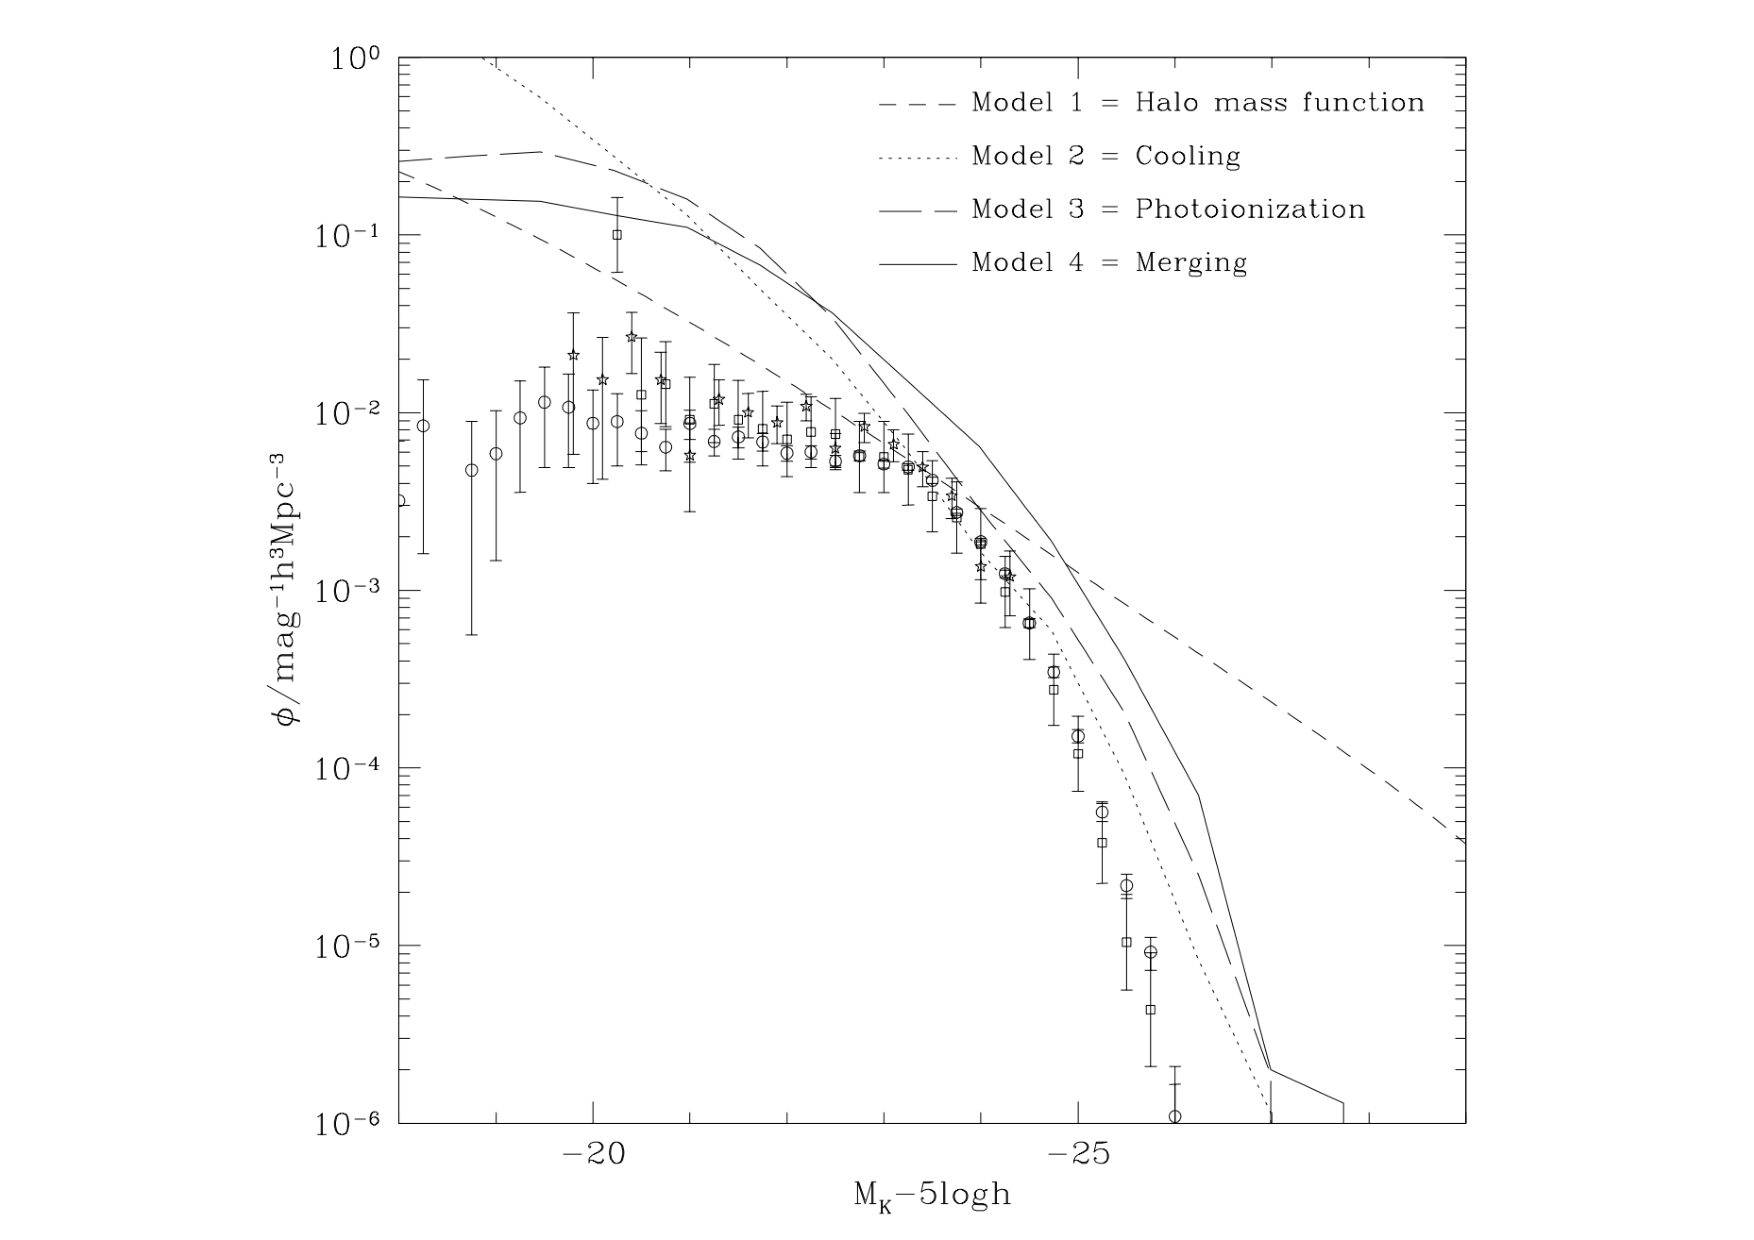
\includegraphics[width=\textwidth]{agn/fig7.pdf}}
\caption[Galaxy luminosity function from observations and simulations: Figure 1 of \cite{benson03}]{Figure 1 from \cite{benson03} showing the K-band luminosity function of galaxies, with $h=0.65$. The points show the observational determinations of \cite[][circles]{cole01}, \cite[][squares]{kochanek01}, and \cite[][$z < 0.1$, stars]{huang03}. Lines show model results investigated by \cite{benson03} to determine what shapes this luminosity function; they concluded that including prescriptions for AGN feedback (supernova feedback winds) can help match the simulations to the data at the bright (faint) end of the luminosity function. The knee of the function occurs at $M_K -5\log_{10} h \sim 23.5$, which is an approximate stellar mass of $\log_{10}[M_*/M_{\odot}] \sim 10.3$, assuming a mass-to-light ratio of $(M/L)_K = 0.8$ \citep{brinchmann00}.}
\label{lumfunc}
\end{figure*}

This mechanism of AGN feedback was originally proposed to regulate the number galaxies at the bright (or high mass) end of the luminosity function in cosmological simulations (see Chapter \ref{intro}). The shape of the observed K-band luminosity function can be seen in Figure~\ref{lumfunc} \citep[Figure 1 from][]{benson03}, falling away from model estimates below a K-band magnitude of $M_K -5\log_{10} h \sim 23.5$, or above an approximate stellar mass of $\log_{10}[M_*/M_{\odot}] \gtrsim 10.3$, assuming a mass-to-light ratio of $(M/L)_K = 0.8$ \citep{brinchmann00}. However, it is the low and medium mass \textsc{agn-host} populations where this rapid recent quenching is dominant (see left panels Figures~\ref{time} \& \ref{rate}). At first this seems contradictory to the arguments posed to constrain the shape of the luminosity function, but with some thought the two results can be reconciled. 

The knee of the luminosity function is the point at which AGN feedback starts to impact the masses of galaxies; this occurs at $\log_{10}[M_*/M_{\odot}] \gtrsim 10.3$, which lies at the lower edge of the medium mass \textsc{agn-host} population studied here. The quenching observed in the low and medium mass \textsc{agn-host} populations will stop the masses of these galaxies from growing any larger in the future. In turn these now quenched galaxies will contribute to dry mergers, which would otherwise have had high gas fractions; limiting the mass of the merger remnants. The combination of these two effects, caused initially by the quench of a lower mass galaxy by negative AGN feedback, will reduce the number of galaxies which will be able to grow to populate the high mass end of the luminosity function. 

However, there still remains the possibility that the AGN is not the cause of the quenching observed, but merely a \emph{consequence} of an alternative quenching mechanism. This idea is supported by simulations showing that the exhaustion of gas by a merger fuelled starburst could cause such a rapid quench in star formation and in turn also trigger an AGN \citep{Croton06, Wild09, Snyder11, Hayward14}. \citet{Yesuf14} also showed that AGN are more commonly hosted by post starburst galaxies, with the peak AGN activity appearing $\geq 200 \pm 100 ~\rm{Myr}$ after the starburst. Such a SFH is not accounted for in the models presented here (see Section ~\ref{future} for a discussion), however this scenario is still consistent with the results presented in this paper; that AGN which are \emph{currently} active have been detected in host galaxies $\sim 1~\rm{Gyr}$ after the onset of quenching. Solving this issue of \emph{cause} vs. \emph{consequence} will not be possible with the currently available SDSS photometry. The advent of Integral Field Unit (IFU) surveys with many aperture fibres per galaxy per observation (such as the MaNGA \citep{bundy15}, SAMI \citep{croom12} and CALIFA \citep{sanchez12} surveys) will allow this problem to be studied by observing the change in quenching parameters with increasing distance from the galaxy nucleus (see Section \ref{future} for a more detailed discussion). 
 

Not all galaxies in the \textsc{agn-host} and \textsc{inactive} samples are quenching (as seen in Figure \ref{cmdsfms}) with a significant proportion of both the \textsc{agn-host} and \textsc{inactive} samples lying on the star forming `main sequence'. A galaxy can therefore still maintain star formation whilst hosting an AGN. The results presented in Section \ref{results} only reflect the trends for galaxies that have undergone or are currently undergoing quenching within the \textsc{agn-host} population and can therefore be accurately fit by an exponentially declining SFH. This prevalence of star forming AGN host galaxies, combined with the results above allows us to consider that either: (i)  the AGN are the cause of the rapid quenching observed but only in gas-poor host galaxies where they can have a large impact, (ii) the AGN are a consequence of another quenching mechanism but can also be triggered by other means which do not cause quenching, or (iii) the SFR of a galaxy can recover post-quench and return to the star forming sequence after a few Gyr (see recent simulations by \citealt{pontzen16} and \citealt{sparre16}). Further investigation will therefore be required to determine the nature of this quenching (see Section \ref{future} for a discussion of proposed future work).


%%%%%%%%%%%%%%%%%%%%%%%%%%%%%%%%%%%%%%%%%%%%%%%%%%%%%%%%%%%%%%%%%%%%%%%%%
%%%%%%%%%%%%%%%%%%%%%%%%%%%%%%%%%%%%%%%%%%%%%%%%%%%%%%%%%%%%%%%%%%%%%%%%%
%%%%%%%%%%%%%%%%%%%%%%%%%%%%%%%%%%%%%%%%%%%%%%%%%%%%%%%%%%%%%%%%%%%%%%%%%
%%%%%%%%%%%%%%%%%%%%%%%%%%%%%%%%%%%%%%%%%%%%%%%%%%%%%%%%%%%%%%%%%%%%%%%%%
%%%%%%%%%%%%%%%%%%%%%%%%%%%%%%%%%%%%%%%%%%%%%%%%%%%%%%%%%%%%%%%%%%%%%%%%%
%%%%%%%%%%%%%%%%%%%%%%%%%%%%%%%%%%%%%%%%%%%%%%%%%%%%%%%%%%%%%%%%%%%%%%%%%
%%%%%%%%%%%%%%%%%%%%%%%%%%%%%%%%%%%%%%%%%%%%%%%%%%%%%%%%%%%%%%%%%%%%%%%%%
%%%%%%%%%%%%%%%%%%%%%%%%%%%%%%%%%%%%%%%%%%%%%%%%%%%%%%%%%%%%%%%%%%%%%%%%%
%%%%%%%%%%%%%%%%%%%%%%%%%%%%%%%%%%%%%%%%%%%%%%%%%%%%%%%%%%%%%%%%%%%%%%%%%
%%%%%%%%%%%%%%%%%%%%%%%%%%%%%%%%%%%%%%%%%%%%%%%%%%%%%%%%%%%%%%%%%%%%%%%%%
 

\newpage

\section{Bulgeless galaxies hosting growing black holes}\label{intbulgeless}

\emph{The work in the following chapter has been submitted to MNRAS in Simmons, Smethurst \& Lintott (subm.). I was responsible for the data reduction, statistical analysis and assisted in the interpretation of the results.}

%INSERT PARAGRAPH LEADING ON FROM PREVIOUS SECTION

Although the study of large populations of galaxies provides crucial information to constrain the processes governing galaxy evolution, valuable insight can still be discerned from detailed observations of a smaller sample of rare objects. 

The strong correlations that exist between black hole mass and bulge luminosity \citep{marconi03, haringrix04}, velocity dispersion \citep{magorrian98, merrit01, kormendy11, hu08, mcconnell11} and total stellar mass \citep{cisternas11} suggest a co-evolution of a galaxy with it's central super massive black hole (SMBH). Since mergers can grow both bulges and black holes these correlations have been interpreted as the result of a few mergers within a Hubble time \citep{peng07, hopkins08a, jahnke10}. A growing black hole must accrete matter and is therefore observed as an AGN during this time period. Understanding the triggering mechanisms of AGN which kick-start this process of both galaxy and black hole growth and possible subsequent feedback from the AGN, is therefore important. However in Section \ref{agnfeedback}, I presented the argument that disc galaxies currently hosting an AGN could have started quenching at early times with very slow quenching rates, suggesting an alternative to this typical merger driven galaxy-black hole coevolution scenario \citep{hopkins08a}. 

A secular co-evolution of galaxy and black hole has been proposed by previous works \citep{greene10,jingo, cisternas11, simonise, schawinski11, kocevski12} and was investigated by \citet{Simmons13} who studied 13 AGN residing in disc dominated host galaxies, whose accretion histories are assumed to be merger free. In the following work I examine a larger sample of disc galaxies visually identified as bulgeless or disc dominated hosting an AGN and investigate the locations of these galaxies on typical galaxy-black hole scaling relations. Since the disc galaxies in this sample have different dynamical histories to bulge dominated galaxies, their black hole masses are not expected to correlate in the same way to their stellar masses if different dynamical histories lead to different mechanisms for black hole growth. 

%%%%%%%%%%%%%%%%%%%%%%%%%%%%%%%%%%%%%%%%%%%%%%
%
%
\subsection{Observational Data}\label{sec:data}
%
%
%%%%%%%%%%%%%%%%%%%%%%%%%%%%%%%%%%%%%%%%%%%%%%

The goal of this study is to investigate black hole growth in galaxies whose growth histories have been dominated by relatively calm, slow processes. A sample of growing (i.e. active) black holes hosted in disc-dominated galaxies is therefore required. Optimally, the AGN should have broad emission lines to facilitate measurement of black hole masses via well-established relations between line flux and width and black hole masses. Previously, \citet{Simmons13} investigated a sample of 13 pure disc galaxies hosting AGN. The selection method used in that study selected against very massive black holes with unobscured emission: only 2 AGN of 13 showed clear signs of broadened line emission in their SDSS spectra, leading to calculated black hole masses of $4 \times 10^6 \mmsun$ and $1 \times 10^7 \mmsun $. Here the aim is to select AGN hosted in disc-dominated galaxies at all masses with broad emission lines that can be used to calculate black hole masses through virial assumptions (see Section~\ref{sec:bhmass}). Below the methods used to select both a disc dominated AGN sample along with a control sample of typical AGN host galaxies are described.

%%%%%%%%%%%%%%%%%%%%%%%%%%%%%%%%%%%%%%%%%%%%%%
\subsubsection{AGN Selection}
% including where we get AGN luminosities from
%%%%%%%%%%%%%%%%%%%%%%%%%%%%%%%%%%%%%%%%%%%%%%

In order to examine the black hole-galaxy scaling relation for such galaxies, first a sample of unobscured AGN with broad emission lines must be selected, so that black hole masses may be measured from well-established correlations between emission line properties, such as the FWHM of the broadened $H\alpha$ emission line, and black hole masses \citep[e.g.,][]{gh07a, jiang11a,xiao11, peterson14}. 

Unobscured AGN have characteristic colours in multi-wavelength imaging, particularly in X-ray, optical and infrared bands \citep{kauffmann03b, dstern05, goulding09, kauffmann09, aird12, mendez13, azadi16, cowley16, harrison16}. Given the existence of all-sky surveys at many of the wavelengths relevant to the selection of unobscured AGN, it is now possible to construct larger samples of sources identified as unobscured AGN with high likelihood.

An initial sample of AGN was selected using the W2R sample of \citet{edelson12}, comprised of 4316 sources identified using multi-wavelength data from the \emph{Wide-field Infrared Survey Explorer} \citep[\emph{WISE};][]{wright10}, Two Micron All-Sky Survey \citep[2MASS;][]{skrutskie06}, and \emph{ROSAT} all-sky survey \citep[RASS;][]{voges99}. This multi wavelength photometric, all-sky selection, selects unobscured AGN at $>95$ per cent confidence \citep{edelson12}.



%%%%%%%%%%%%%%%%%%%%%%%%%%%%%%%%%%%%%%%%%%%%%%
\subsubsection{Selecting disc-dominated AGN host galaxies}\label{sec:selectAGN}
% including source of optical imagery
%%%%%%%%%%%%%%%%%%%%%%%%%%%%%%%%%%%%%%%%%%%%%%



\begin{figure*}
\centering
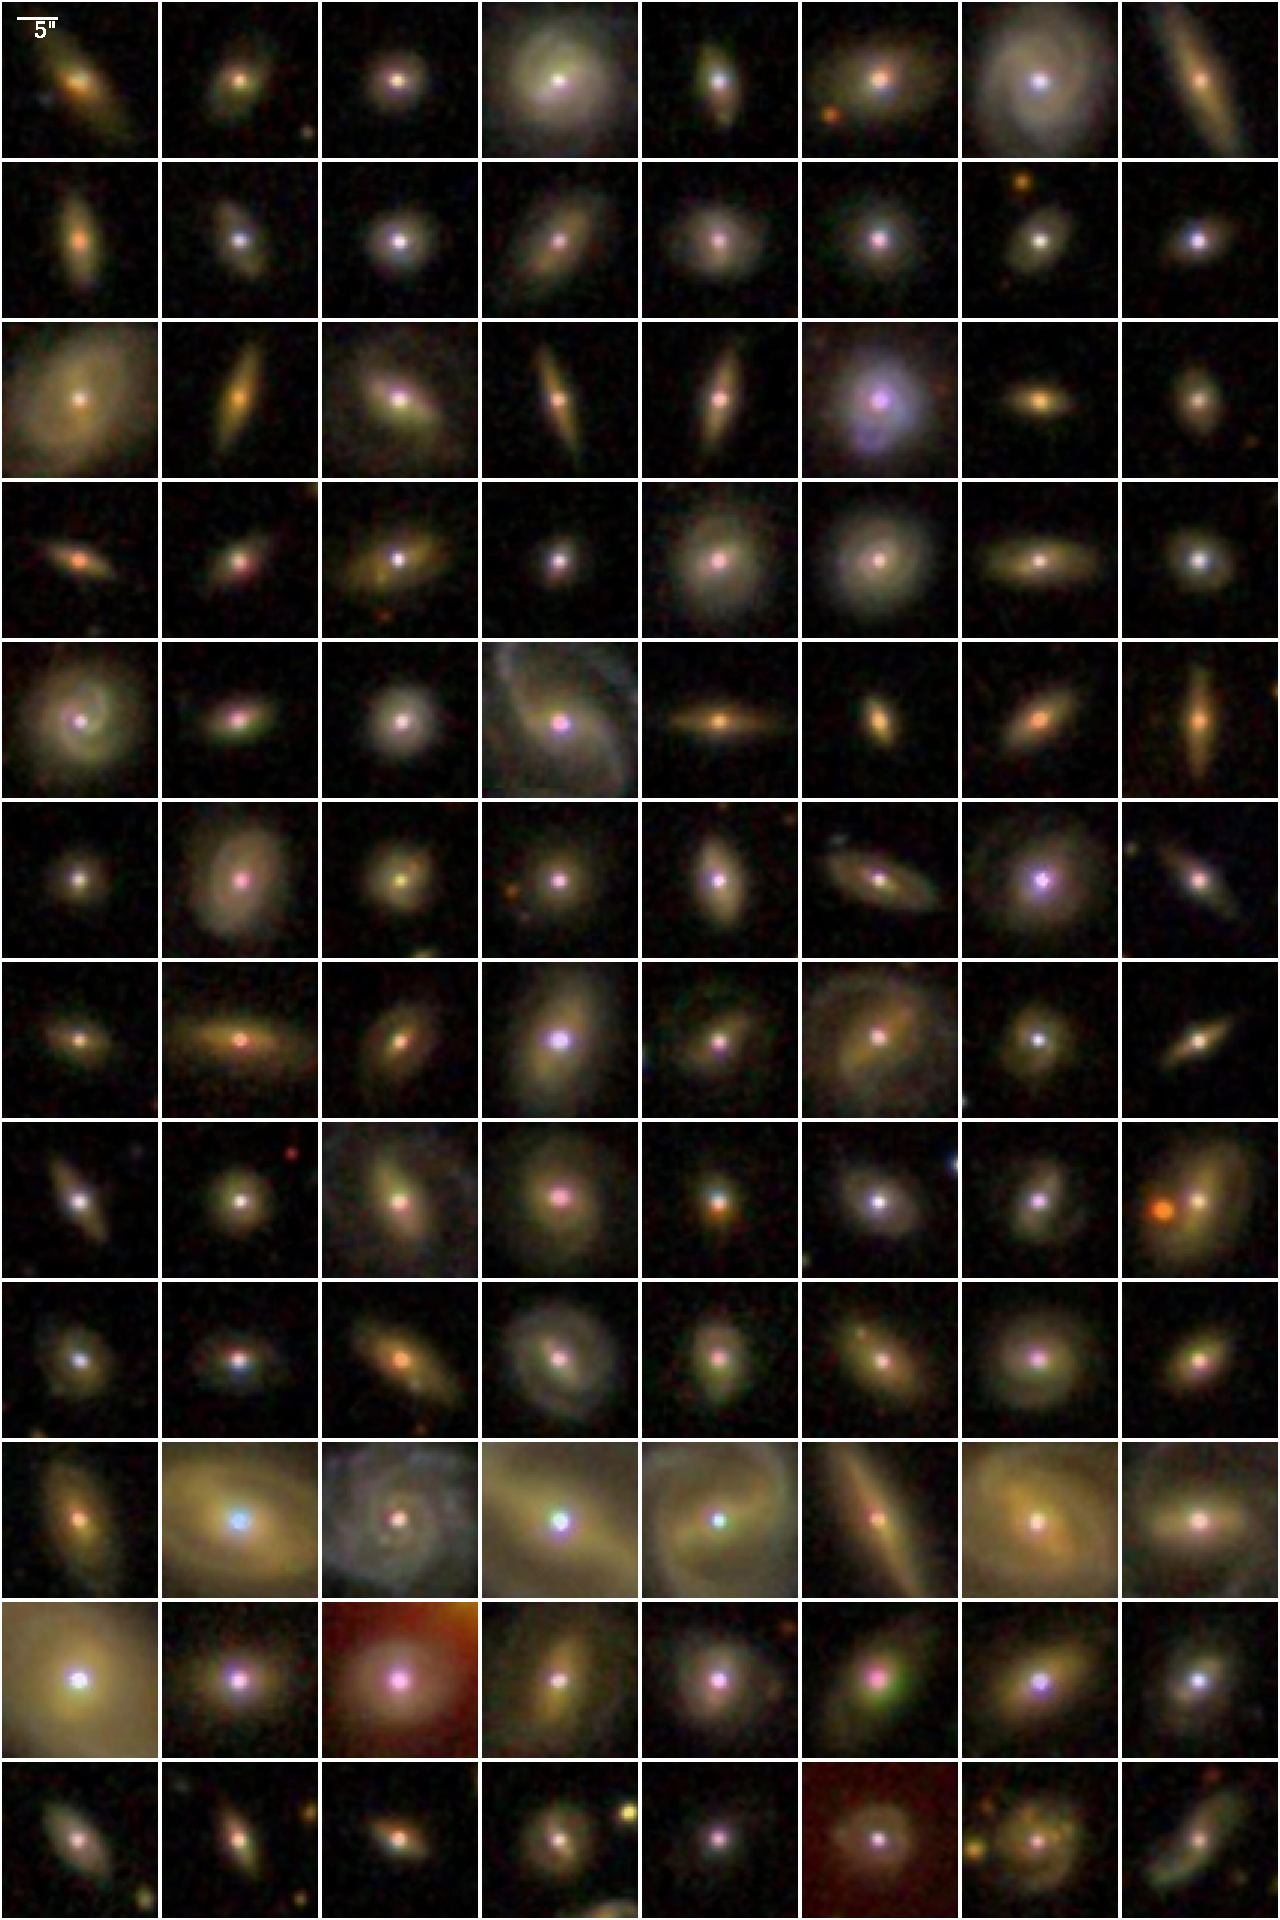
\includegraphics[height=0.9\textheight]{agn/mosaic_all_diskdom.pdf}
\caption[SDSS images of DISKDOM sample]{Postage stamp SDSS images of the $96$ galaxies within the \textsc{discdom} sample for which we have SDSS spectra. The scale for each image is shown by the $5$'' ruler in the top left panel.}
\label{fig:exampleimages}
\end{figure*}


\begin{figure*}
\centering
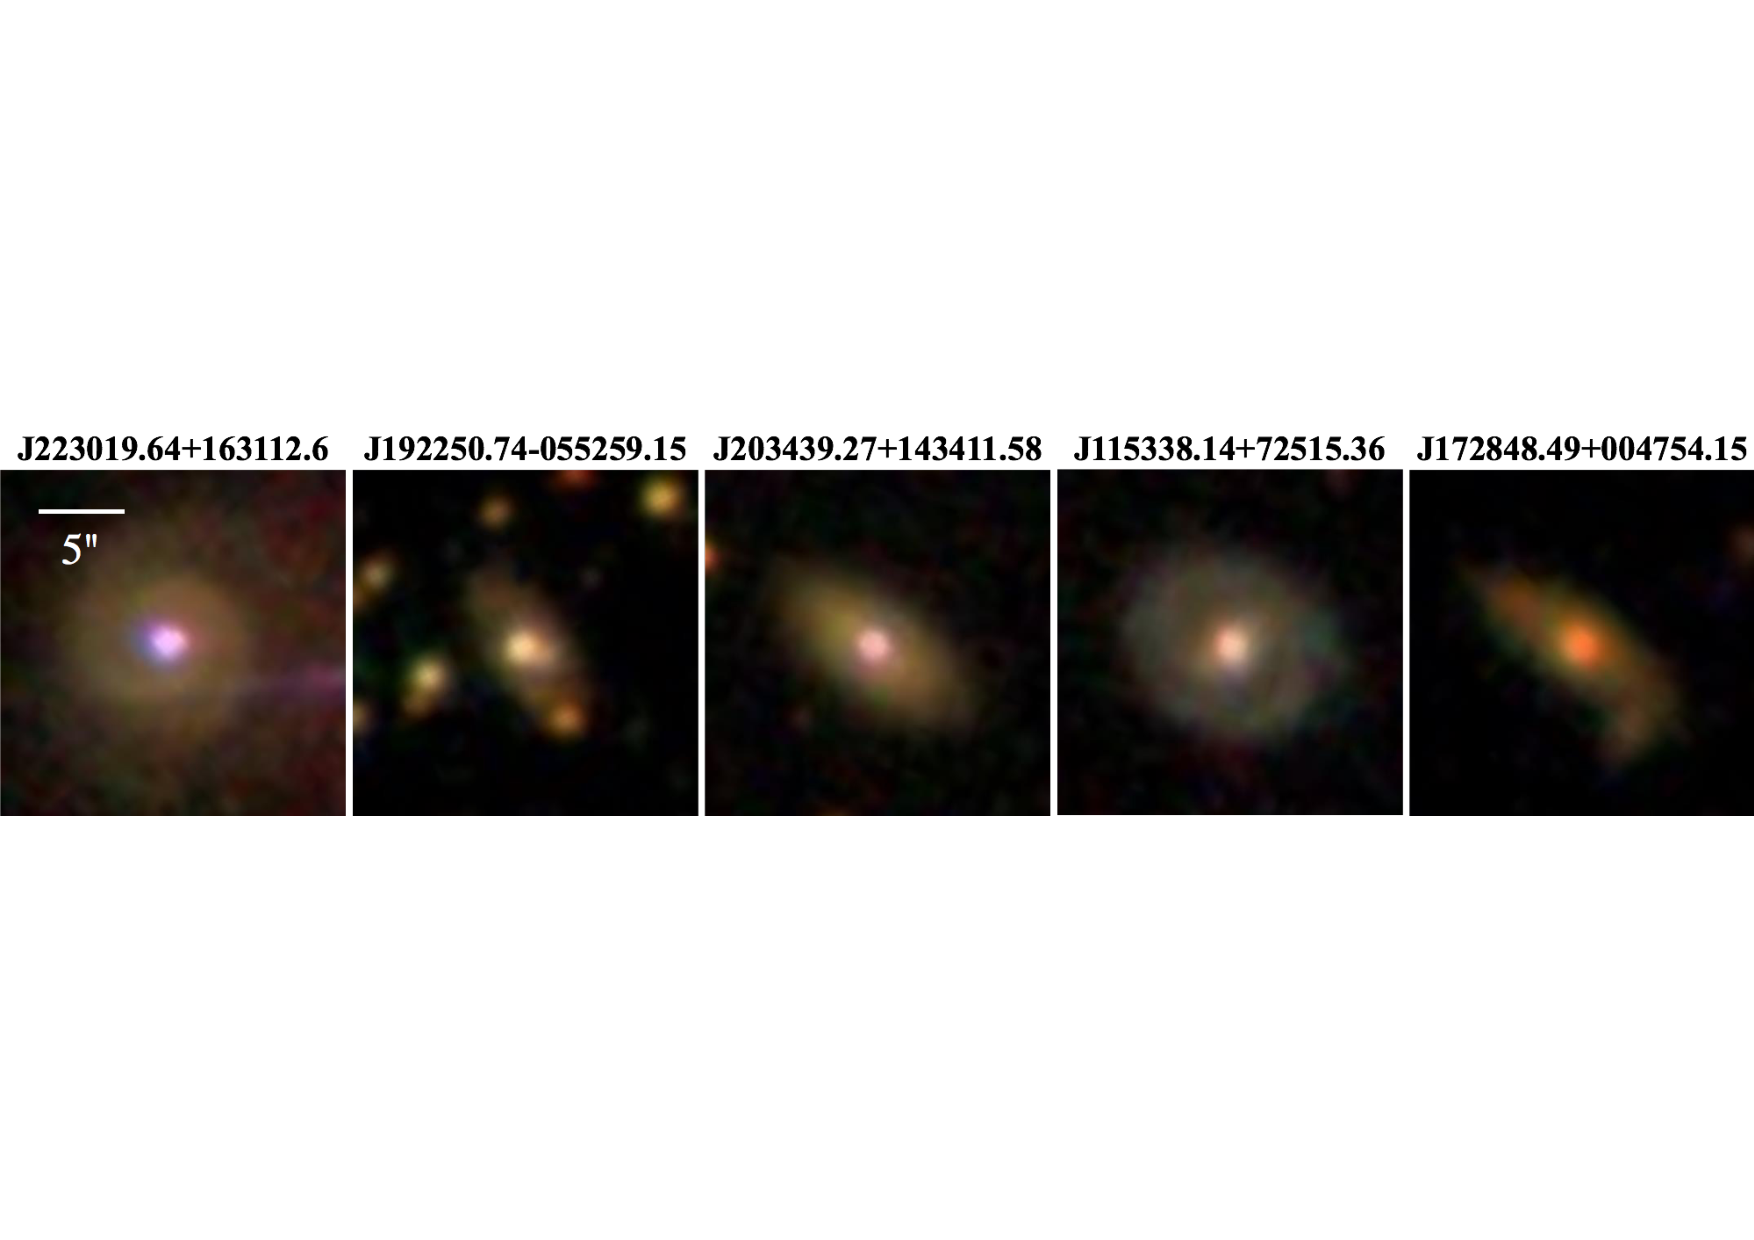
\includegraphics[width=\textwidth]{agn/mosaic_INT_gal_only.pdf}
\caption[SDSS images of 5 galaxies observed with the IDS on the INT]{Postage stamp SDSS images of the $5$ galaxies observed with the IDS on the INT within the \textsc{discdom} sample. The scale for each image is shown by the $5$'' ruler in the left panel.}
\label{fig:INTimages}
\end{figure*}


Following the selection of AGN using the catalog of \citet{edelson12} described in the previous section, galaxies imaged by the Sloan Digital Sky Survey are then further sub-selected. There are 1,844 W2R sources with positional matches having reported coordinates within $3^{\prime \prime}$ of a source in the SDSS \citep{york00} Data Release 8, a fraction consistent with the fractional area of the SDSS versus an all-sky catalog. %76 per cent of this sub-sample have measured redshifts, with a peak redshift distribution of $z \approx 0.12$.  90 percent of sources with redshifts have $z < 0.6$; the distribution has a long tail to $z_{\rm max} = 2.35$.

Each SDSS ugriz colour cutout was then examined to identify disc-dominated features. 101 disc-dominated AGN host galaxies were identified on the basis of clearly identifiable spiral arms, bars or obvious edge-on discs. I shall refer to these galaxies as the \textsc{discdom} sample. Figures~\ref{fig:exampleimages} \& \ref{fig:INTimages} collectively show the SDSS postage stamps for all galaxies in the sample, with all images showing the expected bright nebular emission of the unobscured AGN. 

%%%%%%%%%%%%%%%%%%%%%%%%%%%%%%%%%%%%%%%%%%%%%%
\subsubsection{Spectra}\label{sec:spectra}
%%%%%%%%%%%%%%%%%%%%%%%%%%%%%%%%%%%%%%%%%%%%%%

Of the 101 disc-dominated AGN host galaxies with SDSS imaging observations, 96 have spectra from SDSS Data Release 9 \citep{ahn12}. 23 of which were first identified as AGN by \cite{shen08} and \cite{edelson12}. Example spectra centred around the broad $H\alpha$ emission at $6562\AA$ for 5 of these SDSS spectra are shown in Figure~\ref{fig:SDSSspectra}.

\begin{figure*}
\centering
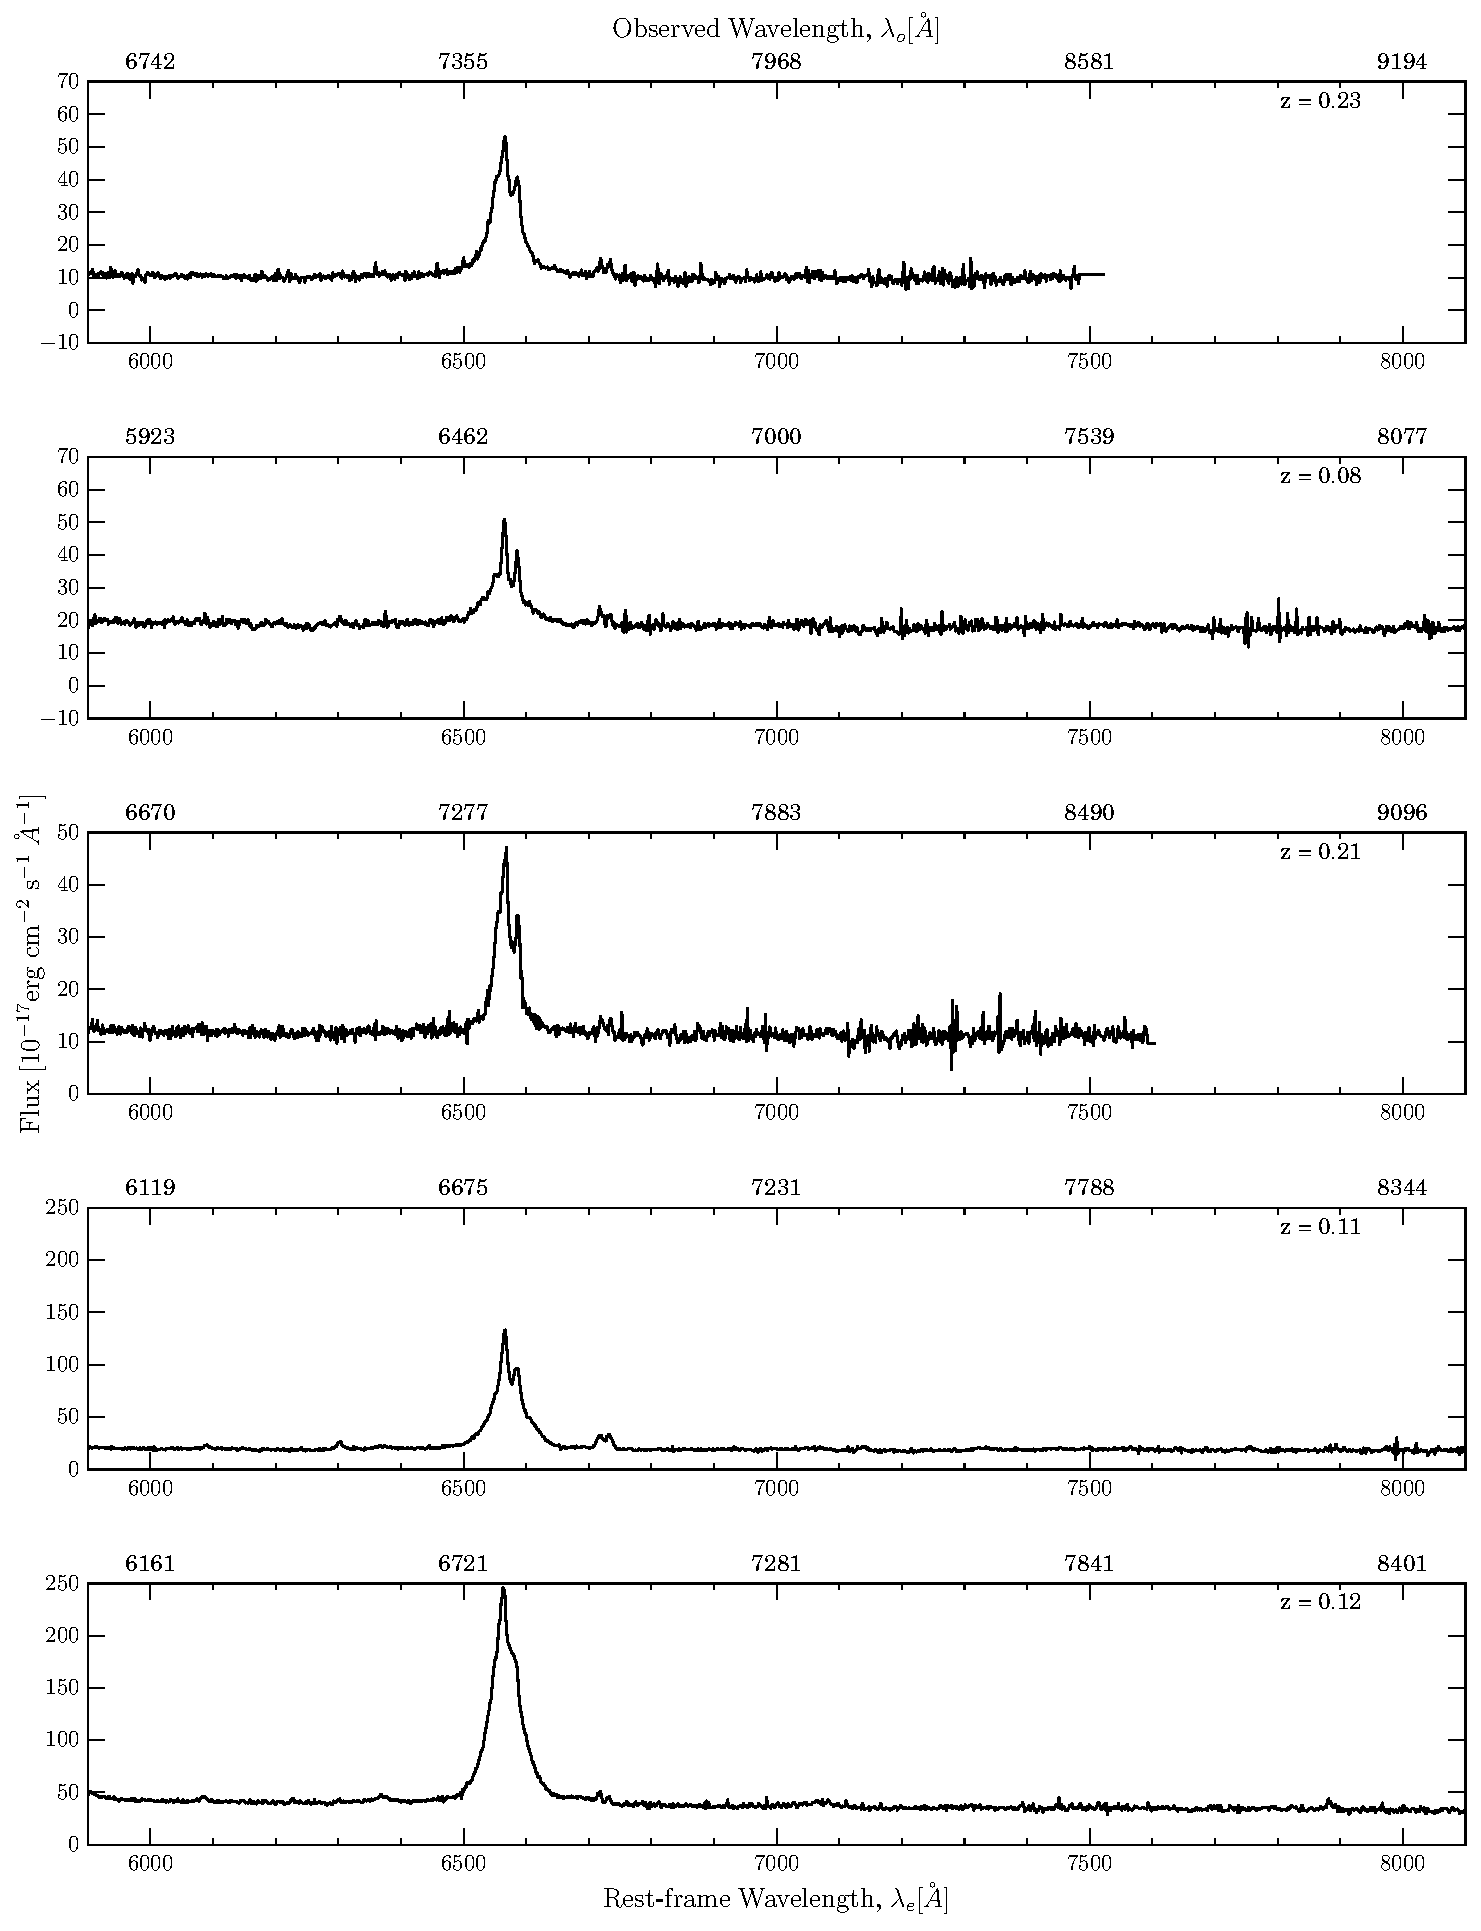
\includegraphics[height=0.8\textheight]{agn/sample_sdss_spectra.pdf}
\caption[Optical SDSS spectra of 5 galaxies in the DISKDOM sample]{5 example SDSS spectra from with the corresponding measured redshift values shown. Each panel shows the same rest-frame wavelength range (bottom axis of each panel); observed wavelengths are shown on the top axis of each panel. All spectra show broadened  $H\alpha$ emission, confirming that the multi-wavelength AGN selection employed here efficiently selects unobscured AGN.}
\label{fig:SDSSspectra}
\end{figure*}

The broad $H\alpha$ emission for  {\notebsm 5 additional sources} were measured using long-slit spectra using Intermediate Dispersion Spectrograph (IDS) on the Isaac Newton Telescope (INT) from 21st-23rd May 2014. I reduced spectra using the standard reduction pipeline of Massey, Valdes \& Barnes (1992) using IRAF modules to debiase, dark subtract, flat field, calibrate, sky subtract, flux calibrate and extract spectra. The redshift of these sources was also measured from the reduced spectra, using the peak of the broadened $H\alpha$ emission to measure $\lambda_{obs}$. These reduced spectra, centred around the broad $H\alpha$ emission at $6562\AA$, are shown in Figure \ref{fig:INTspectra} for the 5 galaxies observed.


\begin{figure*}
\centering
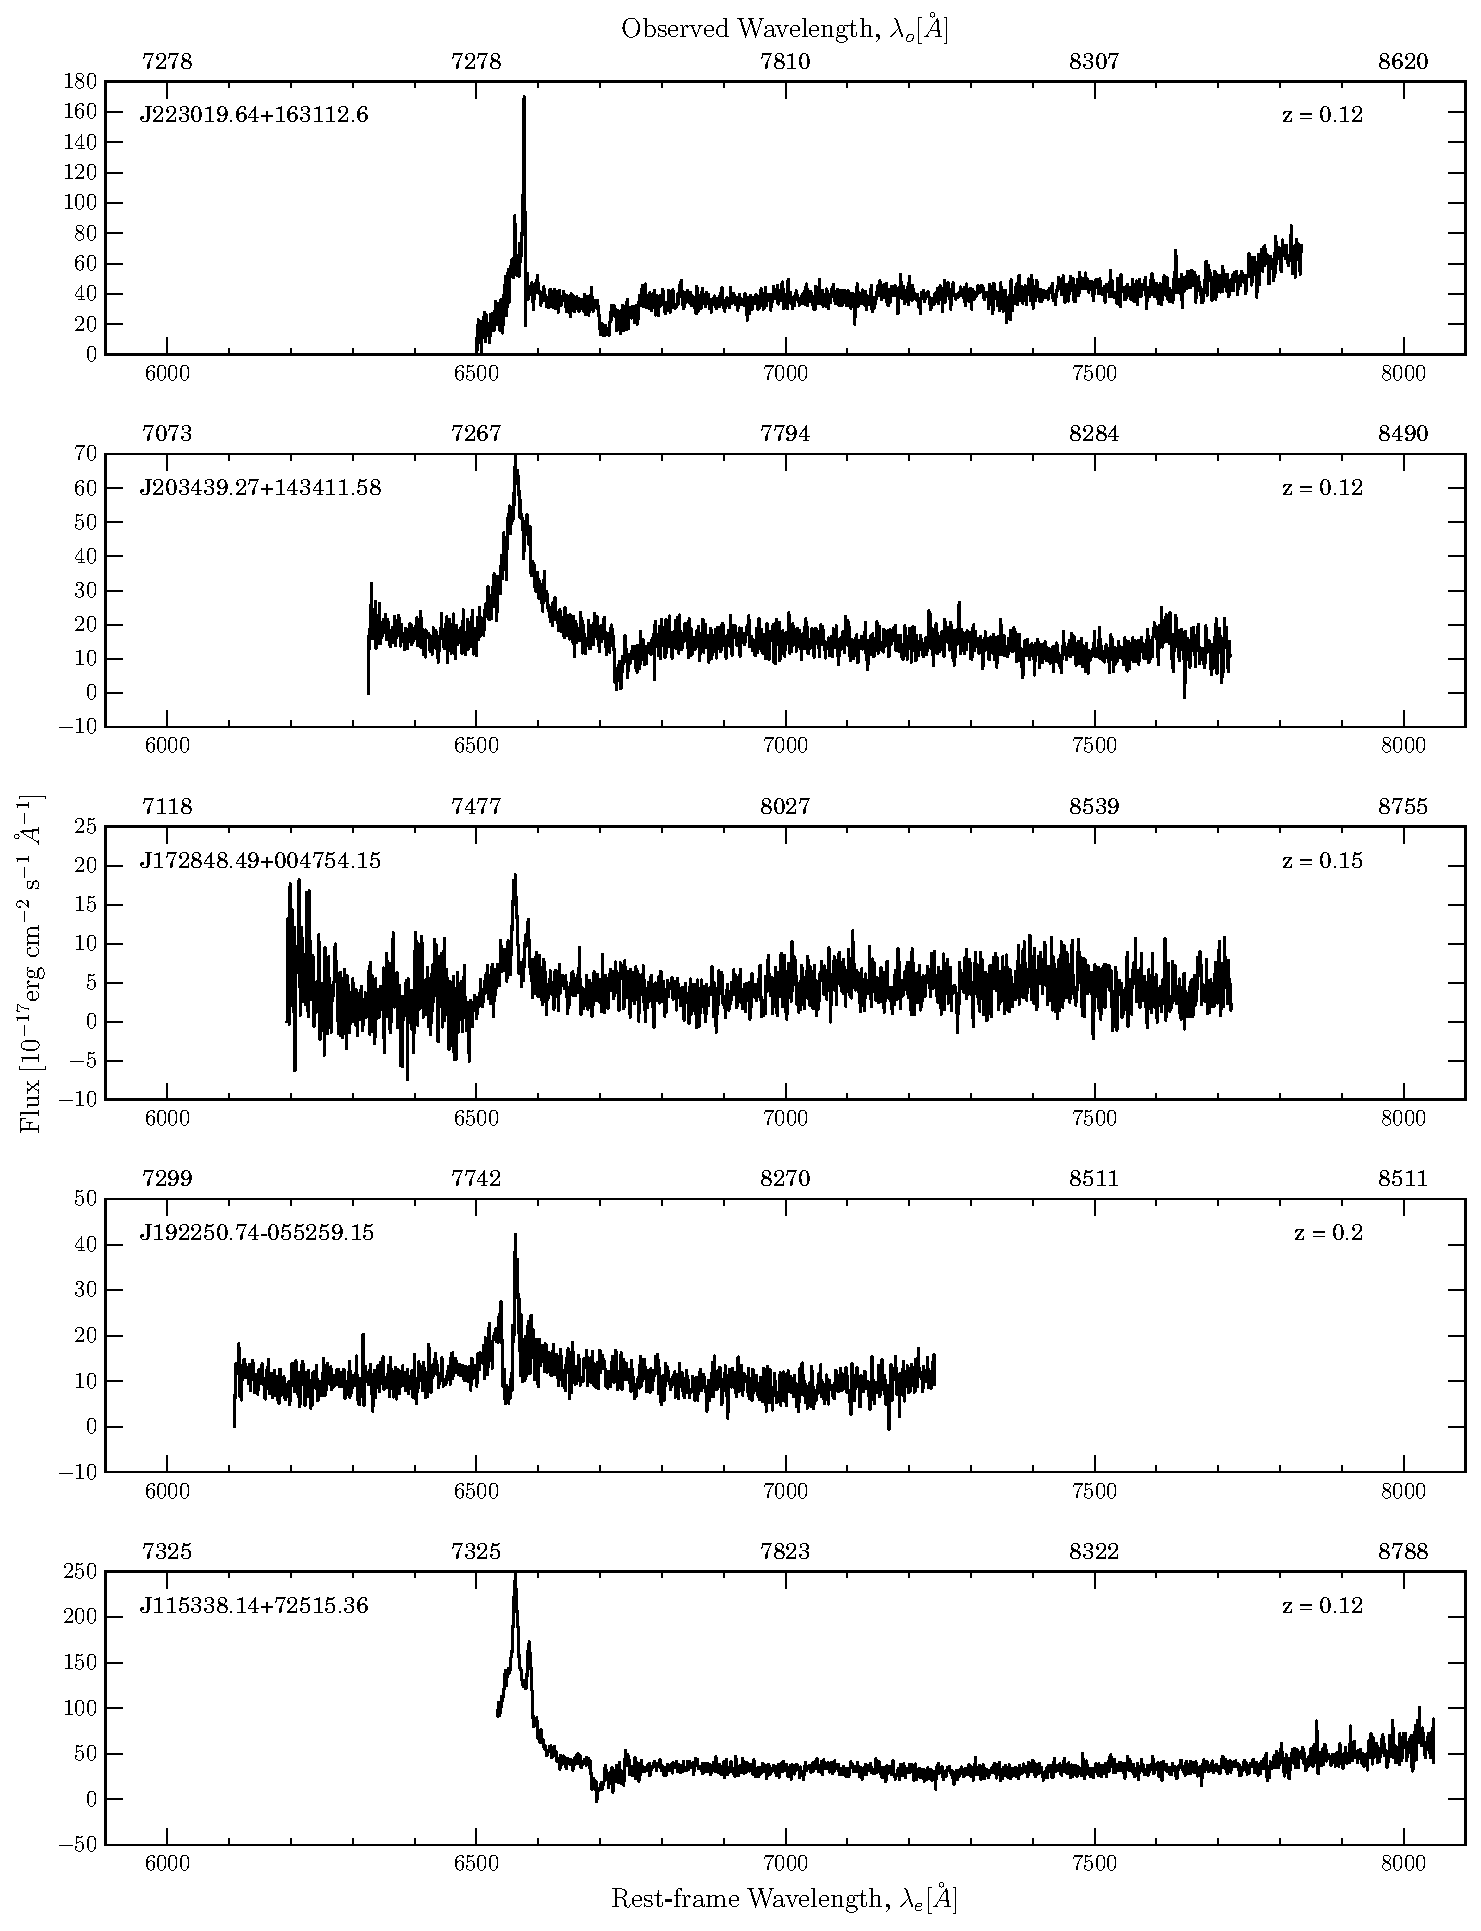
\includegraphics[height=0.8\textheight]{agn/int_spectra.pdf}
\caption[Optical spectra of 5 bulgeless galaxies observed on the INT with the IDS]{Reduced spectra from the IDS on the INT for the 5 galaxies observed. Each panel shows the same rest-frame wavelength range (bottom axis of each panel); observed wavelengths are shown on the top axis of each panel, with redshifts in the top right of each panel. All spectra one again show broadened $H\alpha$ emission, confirming that the multi-wavelength AGN selection employed here efficiently selects unobscured AGN.}
\label{fig:INTspectra}
\end{figure*}

% maybe some details about the spectral resolution?

Figure \ref{fig:redshifts} shows the redshift distribution of all 101 sources for which we have spectra; the mean redshift of the sample is $\left< z \right> = 0.129$, with the highest-redshift source having $z = 0.244$. 


\begin{figure}
\centering
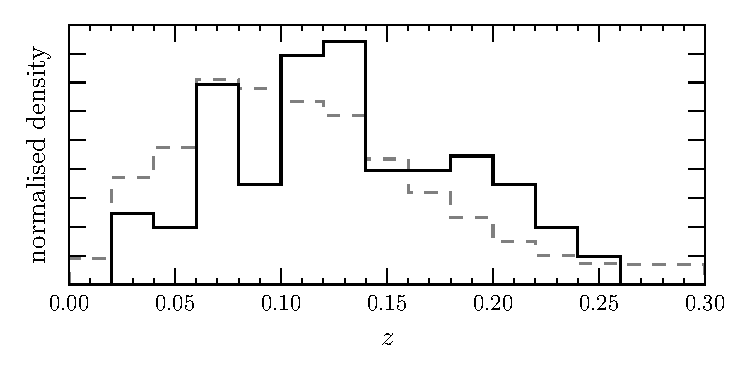
\includegraphics[width=0.9\textwidth]{agn/z_distribution_101_sdss.pdf}
\caption[Redshift distribution of bulgeless galaxies]{Normalised redshift distribution for all 101 sources (solid) for which we have spectra, either from SDSS or measurements with the IDS on the INT. Also shown is the overall redshift distribution of SDSS DR7 in the relevant redshift range of our sources (dashed).
}
\label{fig:redshifts}
\end{figure}

\subsubsection{Selecting a Control Sample}

Since the majority of the galaxies in the \textsc{discdom} sample have been observed using SDSS, I constructed a control sample from the SDSS quasar catalog of \citet{shen11}. Using this sample I compiled a sample of 191 galaxies which were redshift matched to within $\pm5\%$ of the \textsc{discdom} sample. I shall refer to these galaxies as the \textsc{qsocontrol} sample. 124 of the \textsc{qsocontrol} sample also had measured $(B/T)$ ratios from \citet[][matched with a $3''$ search radius, see Section~\ref{sec:galmass}]{simard11}. 

This provides a control sample of `typical' AGN host galaxies representative of the population in the redshift range probed in this study. 

%%%%%%%%%%%%%%%%%%%%%%%%%%%%%%%%%%%%%%%%%%%%%%
%
%
\subsection{Galaxy and Black Hole Properties}\label{sec:masses}
%
%
%%%%%%%%%%%%%%%%%%%%%%%%%%%%%%%%%%%%%%%%%%%%%%

In order to study the relation between galaxy and black hole in these disc dominated systems, their properties shall be compared to well tested black hole-galaxy scaling relations. The most famous of these scaling relations is the $M-\sigma$ relations. This is a well studied relationship \citep{magorrian98, merrit01, kormendy01, tremaine01, marconi01, graham07, graham08, greene10, mcconnell11, beifoiri12, mcconnell13} and is hypothesised to arise due to the merger driven co-evolution increasing the mass of the black hole at the same time as increasing the velocity dispersion of the galaxy \citep{peng07, hopkins08a, jahnke11}. The black hole mass has similarly been found to correlate with the stellar mass of the galaxy bulge \citep{marconi03, haringrix04} and the total galaxy stellar mass \citep{cisternas11}. In order to test where the galaxies of the \textsc{discdom} sample lie in these parameter planes in comparison to `typical' AGN host galaxies, black hole, total and bulge stellar masses were derived for each galaxy. In the following section I describe how this was achieved across the \textsc{discdom} sample. 

%%%%%%%%%%%%%%%%%%%%%%%%%%%%%%%%%%%%%%%%%%%%%%
\subsubsection{Total stellar masses}\label{sec:galmass}
%%%%%%%%%%%%%%%%%%%%%%%%%%%%%%%%%%%%%%%%%%%%%%

Total stellar masses are calculated using the well-studied relation between stellar mass, absolute galaxy $r$-band magnitude, and $u-r$ galaxy colour \citep[corrected for galactic extinction;][]{schlegel98}, following the method of \citet[][see Section \ref{intro}]{Baldry06}. We remove the AGN contribution to the luminosity and colour of each galaxy by subtracting the flux in the SDSS {\tt psfMag} from the flux in {\notebsm {\tt modelMag}}. {\tt psfMag} is the best estimate of unresolved emission, while {\tt modelMag} is the optimal quantity for computing aperture-matched source colours\footnote{https://www.sdss3.org/dr10/algorithms/magnitudes.php}. Uncertainties are propagated from the colour-magnitude relationship and due to the subtraction of the central AGN component. The average uncertainty on each measurement is $\sim0.3\rm{sex}$. The distribution of the stellar masses calculated for the \textsc{discdom} sample is shown in the right panel of Figure~\ref{fig:discdomdist}. 
% not sure if this modelMag vs petroMag vs cModelMag will also be in e.g. Strauss et al. (2002)... must find someone to ask

\subsubsection{Bulge stellar masses}\label{sec:bulgemass}

Calculation of the bulge stellar mass for the \textsc{discdom} sample is more complicated than the stellar mass in the previous section. The nuclear emission (as estimated via comparison of {\tt psfMag} to {\tt modelMag}) is generally between {\notebsm 20 to 200 per cent} of the galaxy-only emission. The presence of the luminous AGN therefore severely compromises the estimates of the bulge-to-total ratio $(B/T)$ in the host galaxy provided by, e.g., the {\tt fracDeV} parameter reported in the SDSS catalogs. The {\tt fracDeV} parameter estimates that $\sim 80\%$ of the galaxies in this sample are pure \citet{devaucouleurs} bulges in the $r$-band, despite the fact that the sample was selected on the basis of clear visual signatures of dominant discs (Figure \ref{fig:exampleimages}). None of the photometric parameters measured by the SDSS pipeline allow for the dual presence of an AGN and a host galaxy. Without such considerations the unresolved AGN light is likely to be attributed to the compact bulge component in a bulge-disc model fit \citep{simmons08,koss11}.


\begin{figure*}
\centering
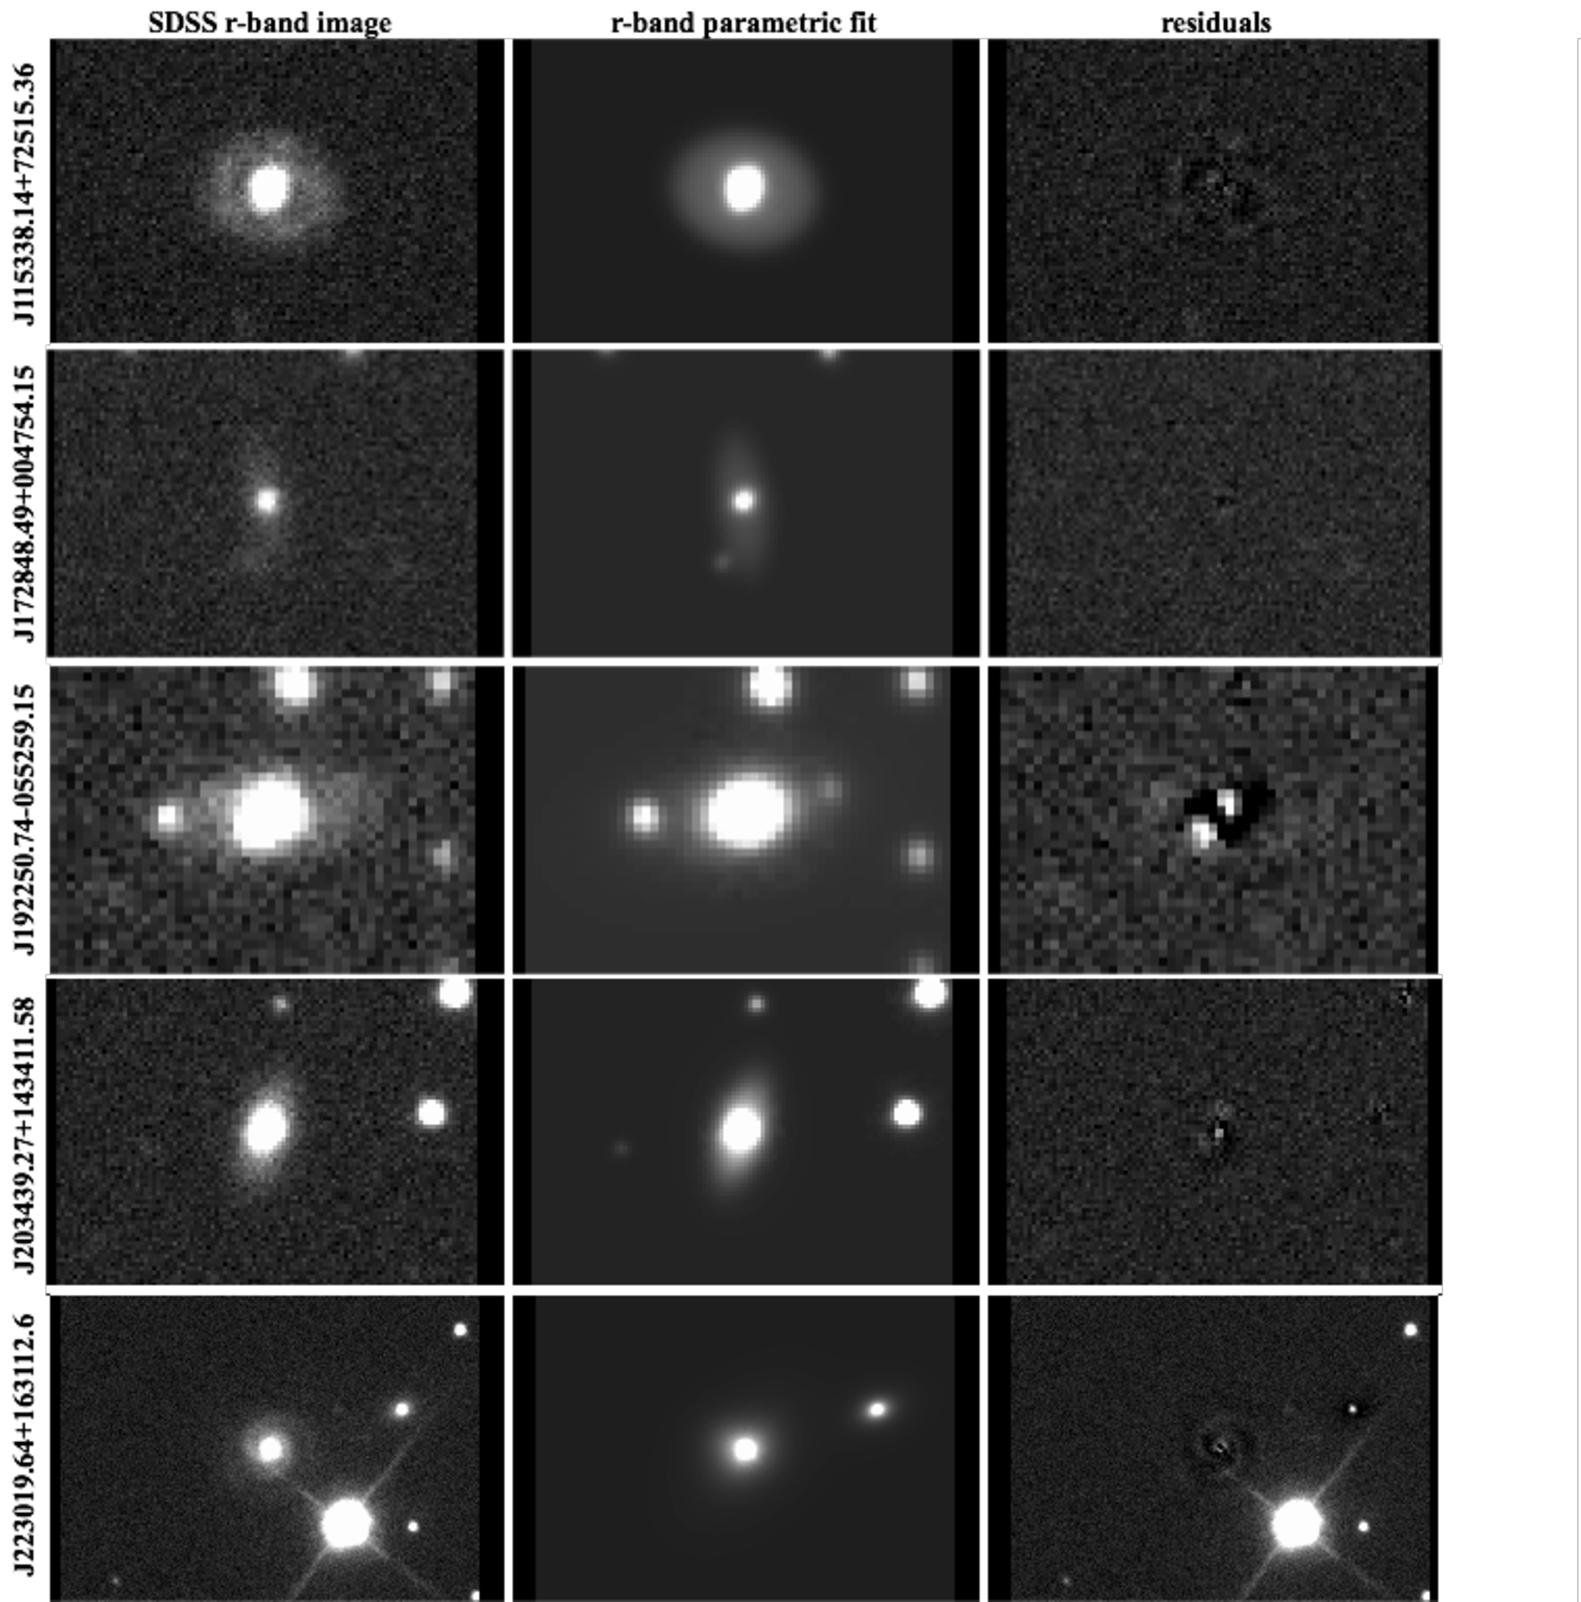
\includegraphics[width=\textwidth]{agn/galfit_residuals.pdf}
\caption[Parametric fits and residuals for the 5 galaxies observed at the INT]{SDSS r-band images (left), with the parametric fits from GALFIT (middle) and the residuals (right; with the same scale as the original image) for the 5 galaxies observed with the IDS at the INT. Stable, but uncertain, bulge-to-total ratios were only recovered for the galaxies in the top two rows. In the bottom three rows the nuclear emission was too bright and resolution too low to derive a reliable estimate of the bulge-to-total ratio.
}
\label{fig:galfit}
\end{figure*}

% wherever the first mention of a pseudo-bulge is, need to \citep{kormendy04}.
AGN-host decomposition based on 2-dimensional image fitting \citep[e.g.,][]{simard98,peng02,peng10} is more reliable \citep[e.g.][]{mclure99,urry00,mclure01,sanchez04,pierce07,gabor09,Simmons11,Simmons13,koss11}. However even in high-resolution \emph{Hubble Space Telescope (HST)} images \citep{simmons08} or SDSS imaging at $z \gtrsim 0.06$ \citep[][]{koss11,simmons13} the recovered bulge-to-total ratio can be highly uncertain, particularly for disc-dominated galaxies with a small bulge or pseudo-bulge \citep{kormendy04} component. While the AGN-host decompositions of the galaxies studied by \citet{simmons13} recovered reliable bulge-to-total ratios for 11 of the 13 galaxies, those sources were at substantially lower redshift than this sample (with the majority at $z < 0.08$), and their AGN were significantly less luminous ($L_{bol} \lesssim 10^{44} \rm{erg}~\rm{s}^{-1}$, whereas in the \textsc{diskdom} sample $L_{bol} \gtrsim 10^{44} \rm{erg}~\rm{s}^{-1}$, see Section~\ref{sec:eddratios}). 

Bulge-to-total fits were first undertaken for the 5 galaxies observed at the INT with the IDS in the \textsc{discdom} sample using the \textsc{galfit} software \citep{peng02}; the results of which are shown in Figure~\ref{fig:galfit}. I used a S\'ersic light profile \citep{sersic68} to model bulge and disc components, defined by an effective radius, $R_e$, and light concentration index, $n$, as:
\begin{equation}\label{sersic}
I(R) = I_e \exp \left(  -b_n \left[  \left( \frac{R}{R_e}\right)^{1/n} -1 \right] \right),
\end{equation}
where $I_e$ is the intensity at the effective radius, $R_e$ and $b_n$ is a constant defined in relation to the s\'ersic index, $n$. Typical disc (bulge) profiles have $n=1$ ($n=3$). Each of the galaxies observed with the INT were fitted with a disc, bulge and PSF component (to account for the bright nuclear emission of the AGN). PSFs were extracted from the SDSS FITS images using the standard \texttt{read\_PSF} IDL code provided by the SDSS \footnote{\url{http://www.sdss.org/dr12/algorithms/read_psf/}}. Initial guesses of $n=2.5$ are used on the first pass of the \textsc{galfit} algorithm, which uses a $\xi^2$ minimisation method to determine the best fit s\'ersic index, effective radius, magnitude and position for each of the components. This first pass allows the positions of the components to be determined, which are then fixed as a second pass of the algorithm is run to ensure the correct magnitudes, radii and s\'ersic indices have been fitted. From these models, the \textsc{galfit} r band magnitudes of the bulge and disc components were converted to fluxes and the bulge-to-total ratio, $(B/T)_r$ was calculated as follows:
\begin{equation}\label{btratio}
(B/T)_r = \frac{10^{(\frac{m_{r, \rm{bulge}}}{-2.5})}}{\left[10^{(\frac{m_{r, \rm{bulge}}}{-2.5})} + 10^{(\frac{m_{r, \rm{disc}}}{-2.5})}\right]}.
\end{equation}

Stable, but highly uncertain, bulge-to-total ratios were recovered for only {\notebsm 2} of the 5 galaxies (the top two galaxies in Figure~\ref{fig:galfit}). In the remaining 3 cases the nuclear emission was too bright and the resolution too low for a reliable bulge-to-disc decomposition.  Detailed AGN-host fits to the SDSS images in the entire sample are therefore not likely to produce useful measurements of bulge masses. \emph{HST} imaging would enable these measurements, and although currently not available for the galaxies in this sample, observations are currently underway in Cycle 24 (ID: 14606). 

Nevertheless, it is possible to constrain the bulge contribution to the host galaxies using existing structural parameters from large-scale studies performing bulge-disc decompositions of SDSS galaxies. While such studies do not account for the presence of an AGN, their tendency to overestimate the bulge-to-total ratio as a result means that bulge masses derived from these quantities may be taken to be conservative upper limits.

\citet{simard11} fit multiple models to 1.12 million galaxies in the SDSS catalog to determine best-fit models and structural parameters for each galaxy. Their $r$-band bulge-to-total ratio {\notebsm of the best-fit model} is taken as an upper limit to the true bulge-to-total ratio of the \textsc{discdom} sample. To convert limits on bulge luminosities to limits on bulge masses, we assume the mass-to-light ratio of the bulge is equal to the mass-to-light ratio of the disc. This is a reasonable assumption for disc-dominated galaxies, where many of the ``bulge'' components are likely to be rotationally-supported pseudo-bulges \citep{kormendy04} with stellar populations similar to that of the disc {\notebsm \citep[e.g.,][]{graham01a}}.

The upper bulge-to-total limits of the 89 galaxies in the \textsc{discdom} sample which were included in the \citeauthor{simard11} study, range from {\notebsm $0.13 \leq \left({\rm B/Tot}\right)_{\rm max} \leq 1.0$, with a mean value of 0.5}. Applying these bulge-to-total limits to the stellar masses computed using the colour-luminosity relation \citep{bell01,baldry06} results in bulge mass upper limits of {\notebsm $3 \times 10^9 \mmsun < {\rm M_{bulge}} < 7 \times 10^{10} \mmsun $}. The distribution of bulge stellar masses for the \textsc{discdom} sample are shown in the middle panel of Figure \ref{fig:discdomdist}

%%%%%%%%%%%%%%%%%%%%%%%%%%%%%%%%%%%%%%%%%%%%%%
\subsubsection{Black hole mass estimates}\label{sec:bhmass}
%%%%%%%%%%%%%%%%%%%%%%%%%%%%%%%%%%%%%%%%%%%%%%



The selection of unobscured AGN facilitates the accurate estimate of black hole masses using a viral assumption. Unobscured AGN have broad emission lines originating from within the black hole sphere of influence; this photoionized broad line region (BLR) can be used as a dynamical tracer of the black hole mass. The viral black hole mass \citep{peterson14} can be expressed simply as:
\begin{equation}\label{eq:virial}
M_{BH} = f \frac{R\Delta v^2}{G},
\end{equation}
where $\Delta v$ is the velocity dispersion of the emitting BLR, which has radius $R$, which is assumed to be spherical and the factor, $f = 0.75$ \citep{netzer90} corrects for this assumption. The velocity dispersion of the BLR can be inferred from the FWHM of a broad line, such as $H\alpha$ or $H\beta$ and the radius from the luminosity of the same broad line. This radius-luminosity relationship is calibrated using the more precise black hole mass measurement technique of reverberation mapping \citep{blandford82, peterson01, barth15} in which the radii are measured based on the observed delay between variations in the AGN continuum and the BLR emission \citep{kaspi05, bentz06}. Masses derived with this virial method, under these simplifying geometric assumptions, have been shown to be accrate to within a factor of $\sim 3$ when compared to masses derived using the $M-\sigma$ method \citep[][and see Section~\ref{agnsample}]{ferarese01, nelson04, onken04}.

Using the $M-\sigma$ relation to calculate black hole masses (as in Section~\ref{agnsample}) is not possible in this case since I am trying to investigate how these galaxies evolve in comparison to the `typical' AGN host galaxy population used to fit the $M-\sigma$ relation. Instead I employ the established relation between the black hole mass and the FWHM and luminosity in the broad \ha\ line defined by \citet{gh07a}:

\begin{equation}\label{greeneho}
M_{BH} = (3.0^{+0.6}_{-0.5}) \times 10^6 \left ( \frac{L_{H\alpha}}{10^{42} ~\rm{erg}~\rm{s}^{-1}} \right )^{0.45\pm0.03} \left ( \frac{\rm{FWHM}_{H\alpha}}{10^{3}~\rm{km}~\rm{s}^{-1}} \right )^{2.06\pm0.06} M_{\odot},
\end{equation}

with the virial method described above. 

To obtain an estimate of the FWHM of the broadened $H\alpha$ lines, I performed spectral fitting on each of the SDSS and INT spectra described in Section \ref{sec:spectra} to recover narrow- and broad-line strengths and widths of the $\mha\ 6563$ \AA\ line, by using \gandalf\ \citep{sarzi06} {\notebsm to fit multiple simultaneous lines as well as the continuum of the spectra}. \gandalf\ is optimised for use with SDSS spectra and so using the program with the INT spectra required minimal data re-formatting. I logarithmically binned and de-redshifted the spectra. {\notebsm From the continuum-subtracted best fit}, I determine the FWHM and line flux of the broad and narrow components of the \ha\ line simultaneously, one again employing \emcee\footnote{\url{dan.iel.fm/emcee/}}, the Python implementation of a Markov Chain Monte Carlo \citep[MCMC;][]{mackay03, gw10} affine invariant ensemble sampler by \cite{emcee13} described in Chapter~\ref{starpy}. 

The uncertainties reported by \emcee\ encapsulate the separation of narrow and broad line components in measurement of the FWHM. The reported uncertainties on black hole masses include this source of uncertainty as well as the reported uncertainties in the black hole-broad line relation \citep{gh07a}. There are other sources of uncertainties, such as those involved in implicitly assuming the fixed geometric correction factor ,$f=0.75$ \citep{netzer90}, for each SMBH, the spectral noise, and the error introduced by assuming a Gaussian line profile for all measured broad lines. Determining uncertainties for the last two is outside the scope of this study; based on visual inspection of the line fits, the first is very small compared to the other uncertainties. These fits to the broad and narrow line \ha \ components in the INT spectra are shown in Figure \ref{fig:zoomspectra}.

The black hole masses for the 101 galaxies of the \textsc{discdom} sample range from {\notebsm $10^6 \mmsun \leq \mmbh \leq 2 \times 10^9 \mmsun$} and the distribution is shown in the left panel of Figure~\ref{fig:discdomdist} in comparison to those from the \textsc{qsocontrol} sample. We compare these black hole masses to galaxy stellar masses and bulge mass upper limits in Section \ref{sec:bhmassrelations} in following Section~\ref{sec:bhmassrelations}. 

\subsubsection{Bolometric Luminosities}\label{sec:eddratios}

Bolometric luminosities are calculated from the wavelength-dependent bolometric corrections of \citet{richards06} using the conversion from the $12\mu m$ infrared luminosities, $ L_{12\mu m}$:
\begin{equation}
L_{bol} \approx 8 \times L_{12\mu m}.
\end{equation}
The infrared luminosity,  $L_{12\mu m}$, is calculated from the WISE W3 magnitudes, $M_{W3}$, for which all of the \textsc{discdom} sources have a detection, as follows:
\begin{equation}
L_{12\mu m} = \left(\frac{4\pi d^2}{10^{-2}~\rm{m}^2}\right)\left( \frac{c}{\lambda}\right) \left(\frac{F_{\nu, 0}}{1\times10^{23}~ \rm{Jy}} \right)10^{\left(\frac{M_{W3}}{-2.5}\right)}.
\end{equation}

These luminosities were then used to calculate Eddington ratios, $\lambda_{Edd}$, for the \textsc{discdom} sample using the method outlined in Section~\ref{agnsample}. 


\begin{figure}
\centering
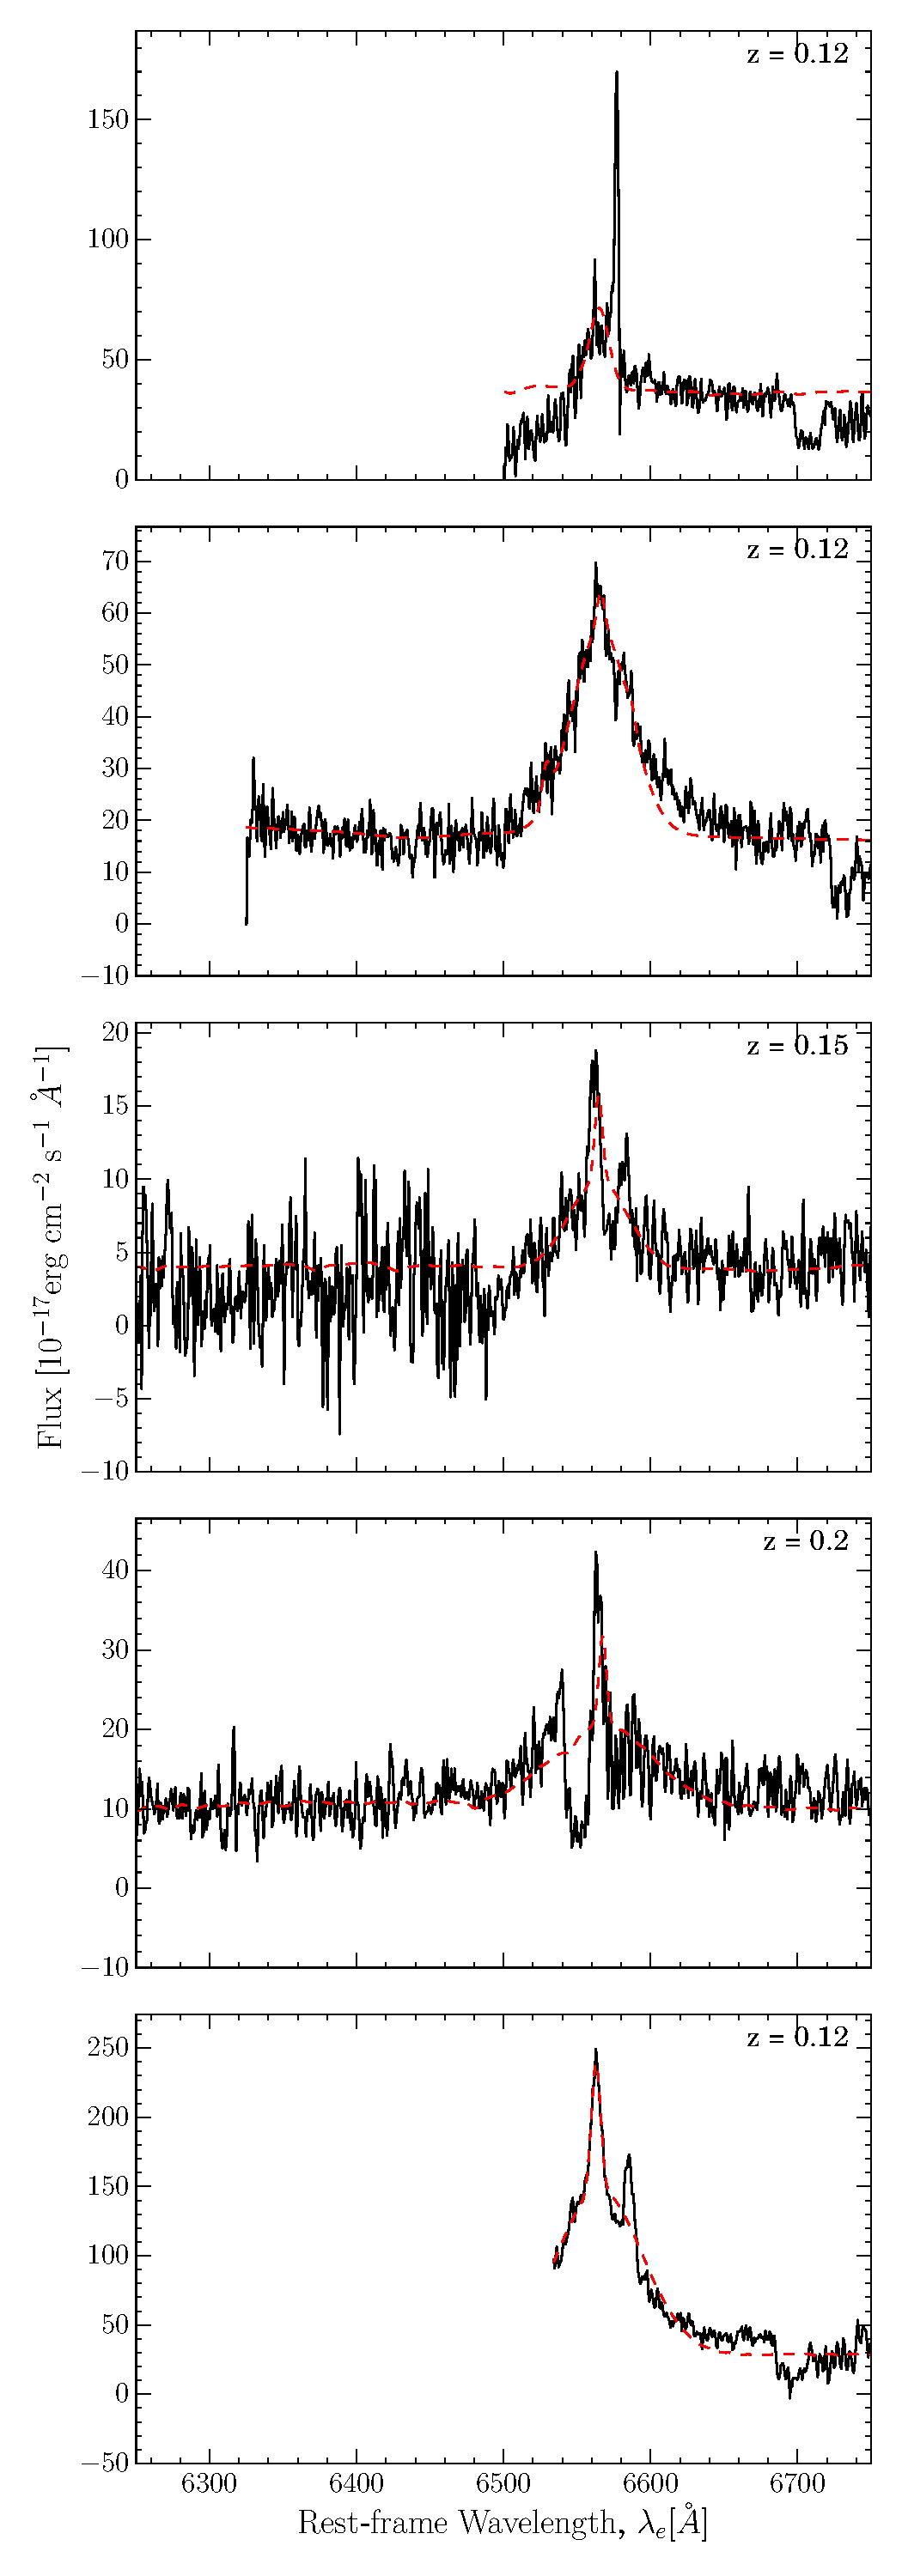
\includegraphics[height=0.9 \textheight]{agn/int_zoom_spectra.pdf}
\caption[Zoom in on $H\alpha$ region of the spectra of 5 galaxies observed with the IDS on the INT]{Reduced spectra from the IDS on the INT for the 5 galaxies observed with the corresponding measured redshift values shown. Spectra are aligned with the broad $H\alpha$ emission line, the gaussian fits to which are shown by the dashed red line.  }
\label{fig:zoomspectra}
\end{figure}



%%%%%%%%%%%%%%%%%%%%%%%%%%%%%%%%%%%%%%%%%%%%%%
%
%  
\subsection{Results}\label{sec:bhmassrelations}
%
% 
%%%%%%%%%%%%%%%%%%%%%%%%%%%%%%%%%%%%%%%%%%%%%%


\begin{figure*}
\centering
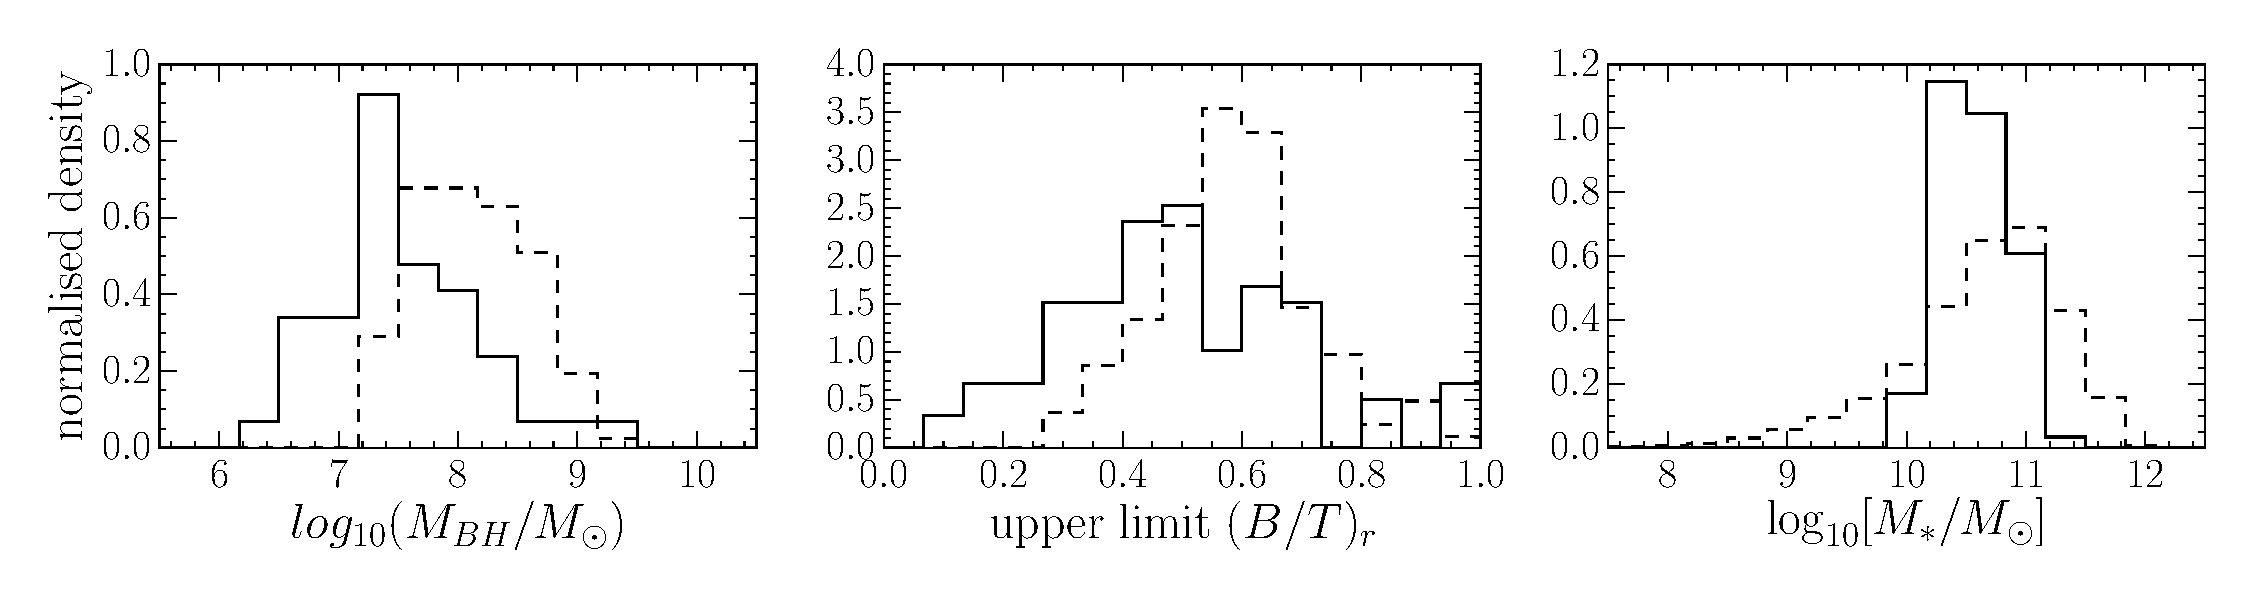
\includegraphics[width=\textwidth]{agn/diskdom_mbh_btot_stellar_mass_distributions.pdf}
\caption[Galaxy and black hole properties of the \textsc{discdom} sample in comparison to the \textsc{qsocontrol} sample]{Distributions of black hole mass (left), upper limits on the r-band bulge-to-total mass ratio from \citet[][middle]{simard11} and stellar mass (right) of the \textsc{discdom} sample (solid) in comparison to the \textsc{qsocontrol} sample (dashed).}
\label{fig:discdomdist}
\end{figure*}

\begin{figure*}
\centering
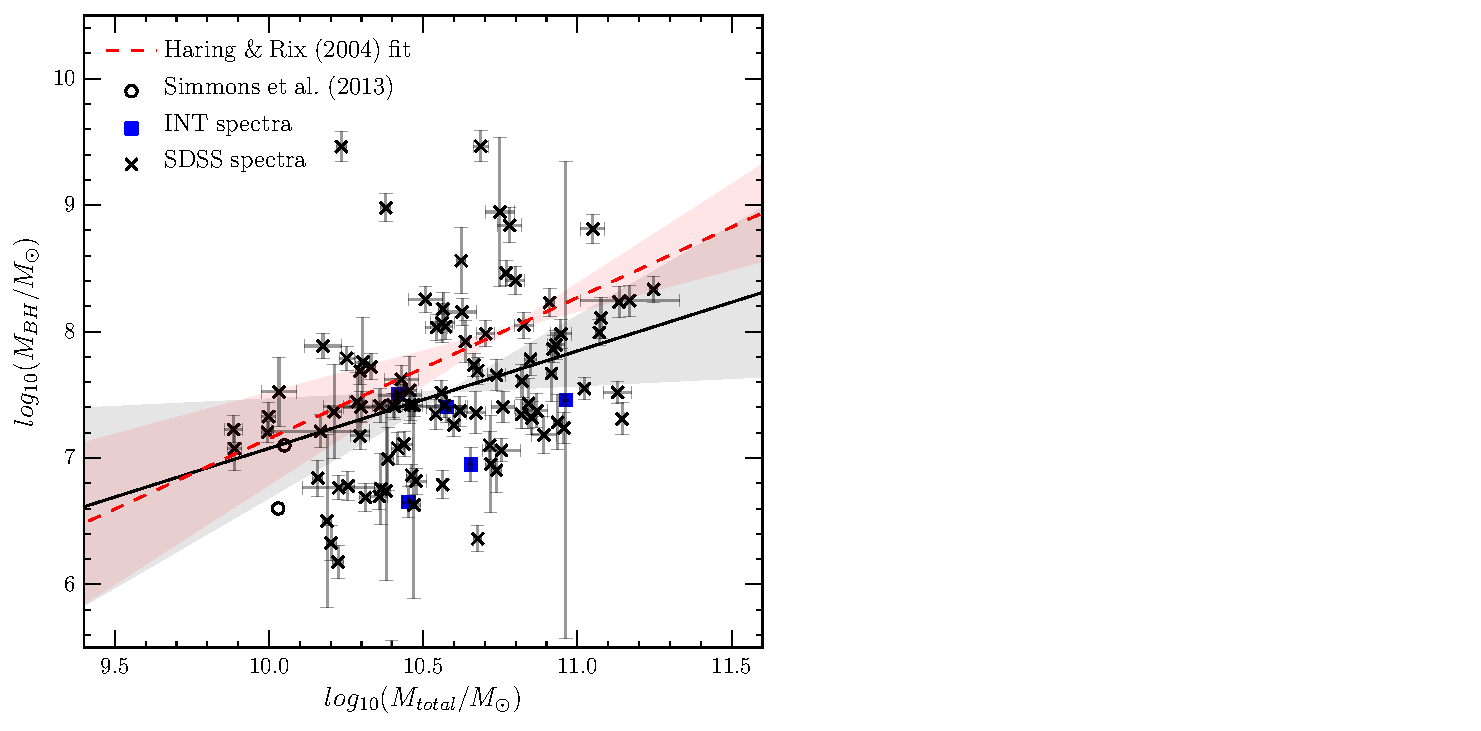
\includegraphics[width=\textwidth]{agn/mass_bh_total_mass_fit_linmix_fit.pdf}
\caption[Black hole stellar mass relation for the \textsc{discdom} sample]{Total stellar mass against the black hole mass of the 101 galaxies, including those observed by SDSS (crosses), with the IDS on INT (blue squares) and detections from \citet[open cirlces]{Simmons13}. The best fit line to the data points and two-dimensional errors from linear regression is shown (solid line) with $\pm3\sigma$ (grey shaded). I also show the best fit found using this same method to the early-type galaxies of \citet{haringrix04} (dashed line) with $\pm3\sigma$ (red shaded) and the measured values shown by the red circles. Despite the fact that these galaxies are predominantly disc dominated they will are most likely to lie above the \citet{haringrix04} relationship found for bulge dominated systems (see discussion in Section \ref{sec:bhmassrelations}).
}
\label{fig:totvsbh}
\end{figure*}

\begin{figure*}
\centering
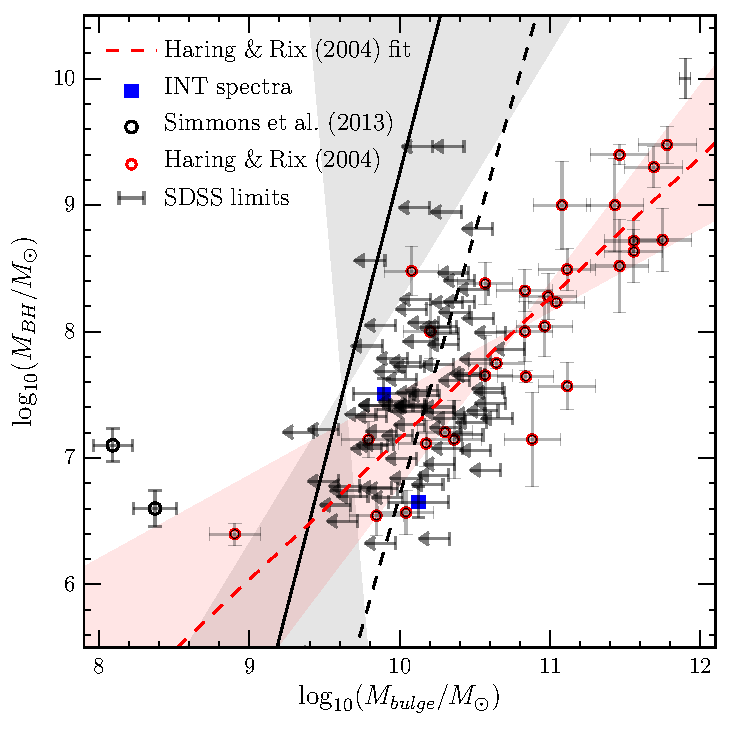
\includegraphics[width=\textwidth]{agn/mass_bh_bulge_limits_INT_simmons13_measurements_linmix_fit.pdf}
\caption[Black hole bulge mass relation for the \textsc{discdom} sample]{The upper limits on the calculated bulge masses are plotted against the black hole mass with the best fit to these upper limits and two-dimensional errors using linear regression methods (solid line) shown with $\pm3\sigma$ (grey shaded). The dashed line shows the fit if the upper limits are not treated as such. I also show the best fit found using this same method to the early-type galaxies of \citet{haringrix04} (dashed line) with $\pm3\sigma$ (red shaded) and the measured values shown by the red circles. Despite the fact that these galaxies are predominantly disc dominated they will are most likely to lie above the \citet{haringrix04} relationship found for bulge dominated systems (see discussion in Section \ref{sec:bhmassrelations}).
}
\label{fig:bulgevsbh}
\end{figure*}


 
The total stellar mass and estimated bulge masses (see Section \ref{sec:galmass}) are shown against the black hole masses for the \textsc{discdom} sample in Figures~\ref{fig:totvsbh} \& \ref{fig:bulgevsbh} respectively. I fit a linear regression model to both of these relations using an inference method which encompasses the uncertainties on both $x$- and $y$-dimensions and the intrinsic scatter in the data. The full method is outlined in \citet{kelly07} and is publicly available as a \emph{Python} module \textsc{linmix}\footnote{\url{http://linmix.readthedocs.org/}}; a brief outline of the method is provided below. The linear regression model assumes:
\begin{equation}\label{2dlinemodel}
\eta = \alpha + \beta * x_i + \epsilon
\end{equation}
\begin{equation}\label{2dlinemodel2}
x = x_i + x_{err}
\end{equation}
\begin{equation}\label{2dlinemodel3}
y = \eta + y_{err}
\end{equation}
Here $\alpha$ and $\beta$ are the regression coefficients, $\epsilon$ is the intrinsic random scatter about the regression, $x_{err}$ is the measurement error in $x$, and $y_{err}$ is the measurement error in $y$. $\epsilon$ is assumed to be normally-distributed, centred around zero, with a variance $\sigma^2$. $x_{err}$ and $y_{err}$ are also assumed to be normally-distributed and centred around zero with variances $\sigma_x^2$ and $\sigma_y^2$, respectively and covariance $xy_{cov}$. The distribution of $x_i$ is modelled as a mixture of normal distributions, with group proportions $\pi$, means $\mu$, and variances $\tau^2$. This linear regression method can also incorporate the upper limits on the bulge mass measurements of the 89 SDSS galaxies measured by \citet[][see Section \ref{sec:galmass}]{simard11}, which is shown by the solid line in Figure~\ref{fig:bulgevsbh}.

Using \textsc{linmix}, I also fit to the observations of 30 early-type galaxies from \citet{haringrix04}. Despite the fact that galaxies in the \textsc{discdom} sample are disc dominated and contain either a pseudo-bulge or no bulge, they preferentially lie above the relationship between black hole and bulge stellar mass derived using the bulge dominated galaxies of \citet{haringrix04}, as seen in Figure~\ref{fig:bulgevsbh}. 

I consider how the black hole mass compares to the Eddington ratio, or accretion rate, of these disc dominated galaxies and compared with the \textsc{qsocontrol} sample in Figure \ref{fig:mbhvsbol}. The galaxies of the\textsc{discdom} sample have both lower black hole masses and lower bolometric luminosities in comparison to the \textsc{qsocontrol} sample, however the Eddington ratio's are very similar, see Figure \ref{fig:eddratioshen}. In fact, the Eddington ratio's of the redshift matched sample are on average, lower than that for the \textsc{discdom} sample. I can reject the null hypothesis that the disc dominated galaxies are drawn from the same distribution as the \textsc{qsocontrol} sample but not for the entire quasar sample of \citet{shen11}.

Within the \textsc{qsocontrol} sample, 108 galaxies were morphologically classified by the Galaxy Zoo 1 project \cite{lintott08, Lintott11}, all of which have a debiased combined spiral vote fraction (Galaxy Zoo 1 did not ask whether a galaxy was a disc, therefore we can approximate the combined spiral vote fraction as a disc vote fraction) of $p_{CS} < 0.5$ and mean value of $\left<p_{CS} \right> = 0.17$.  The \textsc{qsocontrol} sample is therefore mainly comprised of bulge dominated galaxies unlike the \textsc{discdom} sample. 

Slightly higher accretion rates are therefore occurring in the AGN of the galaxies in the \textsc{discdom} sample than in a bulge dominated \textsc{qsocontrol} sample. 

\begin{figure}
\centering
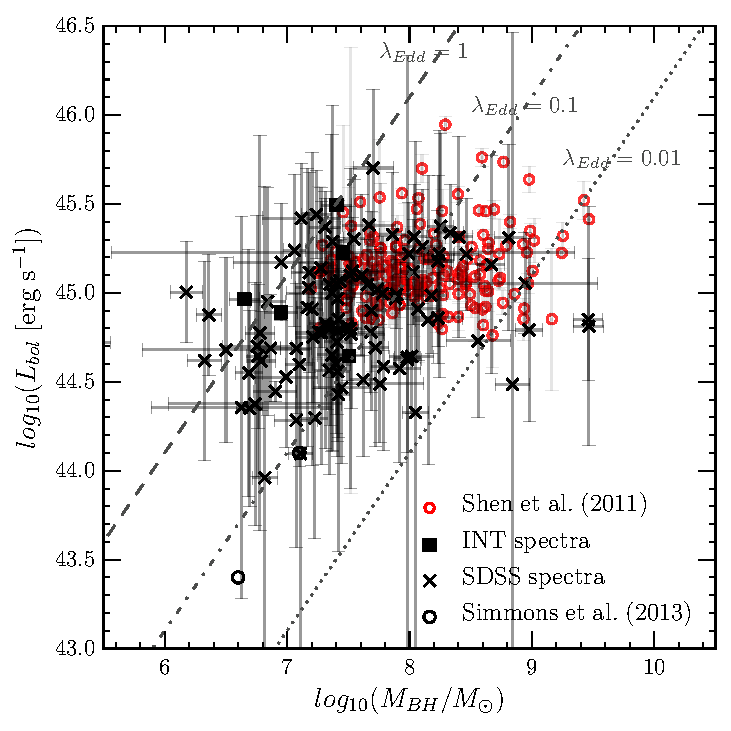
\includegraphics[width=\textwidth]{agn/mass_bh_bol_luminosity_with_all_errors_shen_11.pdf}
\caption[Black hole mass against luminosity for the bulgeless AGN sample]{Black hole mass against bolometric luminosity for the 101 galaxies, including those observed by SDSS (crosses) and with the IDS on INT (squares). We also show detections from {\notebsm Simmons et al. (2013)} (open circles) and those from the redshift matched sample of {\notebsm Shen et al. (2011)}. For reference we show lines of example Eddington ratios of $\Lambda_{Edd}$ = 1 (dashed),  $\Lambda_{Edd}$ = 0.1 (dot-dashed) and $\Lambda_{Edd}$ = 0.01 (dotted).
}
\label{fig:mbhvsbol}
\end{figure}

\begin{figure}
\centering
\includegraphics[width=0.8\textwidth]{agn/edd_ratio_z_matched_shen_2011_compare.pdf}
\caption[Eddington ratio distribution of the bulgeless AGN sample]{Normalised distributions of logarithmic Eddington ratio for the sample of 101 disc dominated galaxies (solid line), compared with that for the redshift matched sample from Shen et al. (2011; dashed line) and the entire sample (dot-dashed line) We also provide the p-values of a 2 sample KS test between the disc dominated sample and each of the quasar samples. We reject the null hypothesis that the two samples are drawn from the same population for the redshift matched quasar sample but accept the null hypothesis for the entire quasar sample of \citet{shen11}.  
}
\label{fig:eddratioshen}
\end{figure}


%%%%%%%%%%%%%%%%%%%%%%%%%%%%%%%%%%%%%%%%%%%%%%
%
%  
\subsection{Discussion}\label{sec:intdiscussion}
%
%
%%%%%%%%%%%%%%%%%%%%%%%%%%%%%%%%%%%%%%%%%%%%%%


\section{Conclusions}\label{sec:agnconclusion}

\chapter{The influence of the group environment}


\section{Group Identification}\label{sec:groups}

We used the \citet{berlind06} catalogue, which uses a friends-of-friends algorithm to identify group and cluster galaxies in the SDSS. This was cross matched to the \textsc{gz-galex} sample and limited to $z < 0.1$ to ensure GALEX completeness of the red sequence (see \citealt{ref}). Centrals were selected as the brightest galaxy in a group and all others were designated as satellites. This resulted in a sample of $14,199$ group galaxies with $3,468$ centrals and $10,731$ satellites within a projected cluster centric radius range of $0 < R/R_{200} < 25$ and $z < 0.084$. 

In this work we focus on galaxies which are either quenching or quenched and are more than $\pm1\sigma$ below the star forming `main sequence'. This encompasses $4629$ satellite and $2314$ central galaxies and will be referred to as the \textsc{gz-group} sample. {\notebsm These galaxies are highlighted in red on Figure \ref{}. }

\subsection{Field sample}\label{sec:field}

For all galaxies in the \textsc{gz-galex} sample, we calculated the smallest projected cluster centric radii from each of the central galaxies in the  \citet{berlind06} catalog and selected candidate field galaxies as those with (i) $R/R_{200} > 25$ and (ii) $\log\Sigma < -0.8$ from \cite{baldry06}. This sample of field galaxy candidates was then matched in redshift and stellar mass firstly to the central galaxies of the \textsc{gz-group} sample to give $2,309$ field galaxies with $z < 0.084$ which will be referred to as the \textsc{gz-cent-field} sample. Secondly, the field galaxy candidates were then matched in redshift and stellar mass to the satellite galaxies of the \textsc{gz-group} sample to give $6,849$ field galaxies with $z < 0.084$ which will be referred to as the \textsc{gz-sat-field}. These galaxies in the \textsc{gz-sat-field} sample will be used as a control when investigating the morphological trends of satellite galaxies with environment. 

As in Section \ref{sec:groups} we select all those galaxies in the central matched sample $\pm1\sigma$ below the star forming `main sequence', giving $1596$ quenching or quenched field galaxies for use as a control sample, which will be referred to as the \textsc{gz-cent-field-q} sample. These galaxies will be used as a control when investigating the quenching parameters of the different environments in order to ensure that each galaxy under comparison resides in similar stellar mass halos. 
%We also select all those galaxies in the satellite matched sample $\pm1\sigma$ below the star forming `main sequence', giving $$ quenching or quenched field galaxies for use as a control sample, which will be referred to as the \textsc{gz-sat-field-q} sample.
  
\begin{figure*}
\centering{
\includegraphics[width=0.95\textwidth]{environment/mosaic_sat_cent_field_disc_fraction.pdf}
\caption[SDSS images of galaxies in the \textsc{gz-group} and  \textsc{gz-field} samples]{Randomly selected SDSS \emph{gri} composite images of satellite and central galaxies in the \textsc{gz-group} sample in comparison to those from the \textsc{gz-field} sample. All galaxies lie within $0.04 < z < 0.05$ and in the central galaxy mass range $10^{10.5} < M_{*} [M_{\odot}] < 10^{11}$, used as a proxy for halo mass. The galaxies are ordered from least to most featured according to their debiased `disc or featured' vote fraction, $p_d$ (see \citealt{GZ2}). The scale for each image is $0.099~\rm{arcsec/pixel}$.}}
\label{fig:mosaic}
\end{figure*}

\begin{figure}
\centering{
\includegraphics[width=0.8\textwidth]{environment/redshift_cent_field.pdf}
\caption[Redshift distribution comparison of the \textsc{gz-group} sample and matched control \textsc{gz-cent-field-q} sample]{Redshift distributions of quenching or quenched central galaxies in the \textsc{gz-group} sample (black solid line) in comparison to the redshift and mass matched \textsc{gz-cent-field-q} sample (blue dashed line).}}
\label{fig:zcompare}
\end{figure}

\section{Results}\label{sec:results}

\begin{figure}
\includegraphics[width=0.46\textwidth]{environment/p_disc_trend_with_log_radius_field_compare.pdf}
\includegraphics[width=0.46\textwidth]{environment/p_smooth_trend_with_log_radius_field_compare.pdf}
\caption[Mean GZ vote fractions for satellite galaxies with projected cluster centric radius]{Mean GZ vote fraction for disc (top) and smooth (bottom) galaxies in the \textsc{gz-group} sample binned in projected cluster centric radius, normalised by $R_{200}$, a proxy for the virial radius of a group. The shaded region shows $\pm1\sigma$ on the mean vote fraction. The mean vote fraction of the \textsc{field} sample are also shown (blue solid lines) with $\pm1\sigma$ (blue dashed lines).}
\label{fig:morphradius}
\end{figure}

\begin{figure}
\centering{
\includegraphics[width=0.95\textwidth]{environment/bar_fraction_over_disc_trend_with_log_radius_sat_matched_field_cand.pdf}
\caption[Bar fraction of satellite disc galaxies with projected cluster centric radius]{Bar fraction (number of barred disc galaxies over number of disc galaxies) in the \textsc{gz-group} sample binned in projected cluster centric radius, normalised by $R_{200}$, a proxy for the virial radius of a group. The shaded region shows $\pm1\sigma$ on the bar fraction. The bar fraction of the \textsc{gz-sat-field} sample is also shown (blue solid line) with $\pm1\sigma$ (blue dashed line).}}
\label{fig:barradius}
\end{figure}

\begin{figure}
\centering{
\includegraphics[width=0.95\textwidth]{environment/merger_fraction_trend_with_log_radius_compare_sat_field_cand.pdf}
\caption[Merger fraction of satellite galaxies with projected cluster centric radius]{Merger fraction in the \textsc{gz-group} sample binned in projected cluster centric radius, normalised by $R_{200}$, a proxy for the virial radius of a group. The shaded region shows $\pm1\sigma$ on the merger fraction. The merger fraction of the \textsc{gz-sat-field} sample is also shown (blue solid line) with $\pm1\sigma$ (blue dashed line).}}
\label{fig:mergerradius}
\end{figure}

First start with a sanity check - do we reproduce morphology-density relation of \citealt{dressler80}? Figure \ref{fig:morphradius} shows the mean disc and smooth vote fractions from galaxy zoo, binned in projected cluster centric radius (normalised by the approximate viral radius of each group, $R_{200}$). We can see that the mean disc (smooth) vote fraction decreases (increases) from the mean field value (blue line) past $1$ virial radius.

Figure \ref{fig:barradius} shows how the bar fraction (number of barred disc galaxies over the number of disc galaxies) increases towards the centre of the group population suggesting the possibility that the environment may play a role in triggering the disk instabilities which produce a morphological bar \citep{ref, ref, ref}. 

Figure \ref{fig:mergerradius} shows how the merger fraction does not significantly deviate from the field fraction (blue line) until beyond $1$ virial radius. Similarly in Figure \ref{fig:bulgeradius} the left panel shows how those galaxies identified as having no or just noticeable bulges are less common in the inner regions of the cluster (left panel), whereas the fraction of galaxies with obvious or dominant bulges (thought to be grown by mergers;\citealt{ref, ref, ref}) increases with decreasing projected distance from the centre of the cluster 

Figure \ref{fig:sfrradius} shows how the SFR of the \textsc{gz-group} sample declines with decreasing cluster centric distance, significantly below the mean SFR of the \textsc{gz-field} sample shown by the blue dashed line. This is in agreement with the results of \cite{gomez03} who observe the decline in SFR with cluster centric radius in SDSS clusters (see for example, Figure 6 in \citealt{gomez03}). 

With the results from \starpy~ we can look at the time since quenching onset ($\Delta t = t_{obs} - t_{q}$, see Section \ref{}) binned in projected cluster centric radius, normalised by $R_{200}$ (a proxy for virial radius) for satellite galaxies and central galaxies in the \textsc{gz-group} sample, compared with galaxies in the \textsc{gz-field} sample. We can investigate these trends with group properties as shown in Figures \ref{fig:timesinceradius} \& \ref{fig:timesinceradiusvel}. 

If mergers are an important evolutionary mechanism for satellite galaxies, we expect to see a difference in the quenching histories of satellites in groups with a higher number of galaxies, $N_{group}$. However, if we look at the bottom panel of Figure \ref{fig:timesinceradius} we do not see a trend with time since quenching onset with increasing $N_{group}$ for the satellite galaxies. The only place we do see such a trend for the central galaxies. 

Across all the panels in Figures \ref{fig:timesinceradius} \& \ref{fig:timesinceradiusvel} we see a general trend for increasing time since quench with decreasing distance from the centre, which is suggestive that this slight trend is due to an effect of the environment itself. As earlier, in Figures \ref{fig:morphradius}$-$\ref{fig:bulgeradius} significant differences from the field value arise beyond approximately one virial radius. 

In the middle panel of Figure \ref{fig:timesinceradius} however, we do see a clear trend for increasing time since quenching onset with increasing stellar mass for both satellite and central galaxies. This is suggestive of mass quenching among the group galaxy population. This is contrary to previous work suggesting that mass quenching is only of import for central galaxies \citep{ref, ref, ref}. 

In simulations, the three things that are seen to constrain galaxy evolution are redshift, mass and halo mass \cite{ref, ref}. To study the effect that halo mass has on the quenching properties of group galaxies we shall use a proxy for halo mass by splitting by the mass of the corresponding central galaxy of the group.

We investigate the effect of the group halo mass in the top panel of Figure \ref{fig:timesinceradius} where we can once again see a clear trend for increasing time since quenching onset with increasing stellar mass of the group central for both satellite and central galaxies. More massive halos therefore have a greater impact on the star formation rate of their satellites than less massive halos. 

In the bottom panel of Figure \ref{fig:timesinceradiusvel} we split the satellite galaxies of the \textsc{gz-group} sample into bins of relative velocity to their central galaxies. We can see that their is no trend with time since onset of quenching with increasing relative velocity for satellite galaxies, however the trend with decreasing projected group centric radius, seen in each panel in Figure \ref{fig:timesinceradius} is still present. This suggests that any environmental processes causing this quenching are not corrected with satellite velocity.  

\begin{figure*}
\includegraphics[width=\textwidth]{environment/min_max_bulge_fraction_trend_with_log_radius_sat_field_cand.pdf}
\caption[GZ2 bulge fractions of satellite disc galaxies with projected cluster centric radius]{Fraction of galaxies with none/just noticeable bulge classifications (left) and with obvious/dominant bulge classifications (right) in the \textsc{gz-group} sample binned in projected cluster centric radius, normalised by $R_{200}$, a proxy for the virial radius of a group. The shaded regions shows $\pm1\sigma$ on the bulge fractions. The bulge fractions of the \textsc{gz-sat-field} sample are also shown (blue solid lines) with $\pm1\sigma$ (blue dashed lines).}
\label{fig:bulgeradius}
\end{figure*}

\begin{figure}
\includegraphics[height=0.825\textheight]{environment/sfr_trend_with_log_radius_field_matched_blue_dashed_hlines_gomez_03_rv_not_r200.pdf}
\caption[Median SFR of the \textsc{gz-group} sample with projected cluster centric radius]{Median $H\alpha$ derived star formation rates of satellite galaxies in the \textsc{gz-group} sample, binned in projected cluster centric radius, normalised by $R_{200}$, a proxy for the virial radius of a group.  The shaded region shows the SFRs encompassed by $50\%$ of the population in a given bin. The median SFR of the \textsc{gz-sat-field} sample is shown (blue solid line) along with the 25th and 75th percentiles (blue dashed lines).}
\label{fig:sfrradius}
\end{figure}

\begin{figure}
\centering{
\includegraphics[height=0.825\textheight]{environment/time_since_quenching_environment_properties.pdf}
\caption[The time since quenching of the \textsc{gz-group} sample with projected cluster centric radius]{The time since quenching onset ($\Delta t = t_{obs} - t_{q}$) binned in projected cluster centric radius, normalised by $R_{200}$, for satellite galaxies (triangles) split by stellar mass of the corresponding central galaxy (top), stellar mass (middle) and the number of galaxies within the group (bottom). The corresponding values for central galaxies (squares) and galaxies in the \textsc{gz-cent-field} sample (circles) are shown and connected by the dashed lines to aid the reader.}
\label{fig:timesinceradius}}
\end{figure}

\begin{figure}
\centering{
\includegraphics[height=0.825\textheight]{environment/time_since_quenching_v_disp_mu_bins_delv.pdf}
\caption[The time since quenching of the \textsc{gz-group} sample with projected cluster centric radius]{The time since quenching onset ($\Delta t = t_{obs} - t_{q}$) binned in projected cluster centric radius, normalised by $R_{200}$, for satellite galaxies (triangles) split by velocity dispersion (top), stellar mass ratio ($\mu_* = M_*/M_{*,c}$) (middle) and the difference in velocity from the associated central galaxy (bottom). The corresponding values for central galaxies (squares) and galaxies in the \textsc{gz-cent-field} sample (circles) are shown and connected by the dashed lines to aid the reader in the top panel where appropriate.}
\label{fig:timesinceradiusvel}}
\end{figure}


\section{Discussion}\label{sec:disc}

We have shown that mergers are important for centrals not for satellites in the bottom panel of Figure \ref{fig:timesinceradius}, that mass quenching is important for satellites as well as centrals in the middle panel of Figure \ref{fig:timesinceradius} and that larger halos have a stronger environmental effect on their satellites in the top panel of Figure \ref{fig:timesinceradius}. 

The trend that is present in all panels of Figure \ref{fig:timesinceradius} was for increasing time since quenching onset with decreasing projected group centric distance. We argue that this lends more support for quenching caused directly by the environmental; galaxies closer in, fell into the group earlier, as they did so they started quenching and so have a longer time since quenching started to occur. However, as seen in Figure \ref{fig:timesinceradiusvel} there is no trend in the time since quenching onset with the relative velocity of the satellites to their corresponding central. This suggests that whatever environmental mechanism is at play here, it is dependant on the size of the halo, either due to the potential or temperature of the halo, but not dependant on the speed of the satellite as in ram pressure stripping theory. This suggests that ram pressure stripping is not the dominant environmental quenching mechanism. 

\chapter{Discussion}

This is where I blow the lid of quenching. Bring it all together in a big happy family picture. 
\chapter{Conlusions}

Quenching is morphologically dependant. 

AGN may be responsible for some of this quenching.

The environment plays less of a role than typical mass quenching. 


%next line adds the Bibliography to the contents page
\addcontentsline{toc}{chapter}{Bibliography}
%uncomment next line to change bibliography name to references
%\renewcommand{\bibname}{References}
\bibliographystyle{mn2e}
\bibliography{refs}        %use a bibtex bibliography file refs.bib

\end{document}

